\documentclass[b5paper,11pt]{article}
\usepackage[top=12ex, bottom=12ex, left=8ex, right=8ex,showframe=false]{geometry}
\linespread{1.6}
\usepackage[ampersand]{easylist}
\usepackage{fancyhdr}
\pagestyle{fancy}
\lhead{ \fancyplain{}{Yuhao Yang} }
\rhead{ \fancyplain{}{\leftmark} }
\cfoot{ \fancyplain{}{\thepage} }
\usepackage[unicode]{hyperref}
\usepackage{amsmath}
\usepackage{amsfonts}
\usepackage{latexsym}
\usepackage{pifont}
\usepackage{fourier}
\usepackage[dvipsnames,svgnames]{xcolor}
\usepackage{extarrows}
\usepackage{graphicx}
\usepackage{tikz}
\usepackage{pgfplots}
\usetikzlibrary{arrows, positioning, calc, fadings, shapes, snakes, decorations.markings, decorations.pathmorphing}
\usepackage{array}
\usepackage{anyfontsize}
\usepackage[european]{circuitikz}
\usepackage{multirow}
\usepackage{indentfirst}
\usepackage{stmaryrd}
\usepackage{paralist}
\usepackage{enumitem}
\usepackage{framed}
\usepackage{tcolorbox}
\usepackage{easyunits}
\usepackage{wrapfig}
\usepackage{xfrac}
\usepackage{caption}
\usepackage{titletoc}
\usepackage[explicit]{titlesec}
\usepackage[makeroom]{cancel}
\usepackage[bottom]{footmisc}
\usepackage{ifthen}
\usepackage{makeidx}

% % % % % % % % % %

\def\includequestions{0}


% section title style
\titleformat{name=\section}[block]
{\begin{center}\begin{tikzpicture}}
	{\draw[line width=4pt, Gray!70, rounded corners] (0,0) rectangle (12.5,3.2);
		\node at (6.25,2.4) {\Huge\sc\bfseries\textcolor{purple}{Chapter \thesection}};}
	{0pt}
	{\node at (6.25,0.9) {\huge\filright\textcolor{purple}{#1}};}[\end{tikzpicture}\end{center}]

% table of contents sytle
\titlecontents{section}[9pc]
{\addvspace{10pt}%
	\begin{tikzpicture}[remember picture, overlay]%
	\draw[fill=Gray!70,draw=Gray!70] (-4,-0.1) rectangle (-0.8,0.5);
	\node at (-2.4,0.2){\color{white}\Large\sc\bfseries chapter\ \thecontentslabel};%
	\end{tikzpicture}\color{Gray}\hspace*{-10pt}\large\bfseries}%
{}
{}
{\;\titlerule\;\large\sc\bfseries Page \thecontentspage
	\begin{tikzpicture}[remember picture, overlay]
	\draw[fill=Gray!70,draw=Gray!70] (2pt,0) rectangle (6,0.1pt);
	\end{tikzpicture}}%
\titlecontents{subsection}[8.1pc]
{\addvspace{1pt}}
{\contentslabel[\thecontentslabel]{2.1pc}}{}
{\hfill\small \thecontentspage}[]
\titlecontents*{subsubsection}[8.1pc]
{\addvspace{-1pt}\small}{}{}
{\ - \small\thecontentspage}
[ /\ ][]



% font type
\renewcommand*\rmdefault{ppl}
%\newcommand{\dd}{\mathrm{d}}
%\newcommand{\ee}{\mathrm{e}}

% equation box
\makeatletter
\renewcommand{\boxed}[1]{\textcolor{black}{%
\tikz[baseline={([yshift=-.72ex] current bounding box.center)}] \node [thick, rectangle, minimum width=1ex,rounded corners,fill=yellow!30, draw=orange] {\normalcolor\m@th$\displaystyle#1$};}}
\tikzset{nomorepostaction/.code={\let\tikz@postactions\pgfutil@empty}}
\renewcommand\normalsize{%
	\@setfontsize\normalsize\@xpt\@xiipt
	\abovedisplayskip 0\p@ plus 5\p@ minus 3\p@
	\belowdisplayskip 0\p@ plus 5\p@ minus 3\p@
	\abovedisplayshortskip 0\p@ plus 5\p@ minus 3\p@
	\belowdisplayshortskip 0\p@ plus 5\p@ minus 3\p@
	\let\@listi\@listI}
\setlength{\@fptop}{0pt}
\newcommand{\specialcell}[1]{\ifmeasuring@#1\else\omit$\displaystyle#1$\ignorespaces\fi}
\makeatother


% % % % % % % % % %

\DeclareGraphicsExtensions{.eps,.mps,.pdf,.jpg,.png}
\graphicspath{{figures/}}
\renewcommand\thefootnote{\textcolor{blue}{[\arabic{footnote}]}}
\hypersetup{
    colorlinks, linkcolor={purple}, citecolor={blue}, urlcolor={blue},
    pdftitle={Cambridge International A-Level Physics Course Handout},
    pdfauthor={Yuhao Yang},
    pdfsubject={A-Level Physics} }

% tikz arrows
\tikzset{>=stealth', pil/.style={ ->, thick, shorten <=2pt, shorten >=2pt,} }

% tikz decription node style
\tikzset{note/.style={rectangle, rounded corners, minimum size=6mm, draw=black, fill=white, font=\itshape, align=center,execute at begin node=\setlength{\baselineskip}{1.2em}}}
\tikzset{graphlabel/.style={postaction={decorate,transform shape, decoration={markings, mark=at position .5 with \node #1;}}}}
\tikzset{twoline/.style={align=center,execute at begin node=\setlength{\baselineskip}{1.2em}}}
\tikzset{twolinecap/.style={align=center,execute at begin node=\setlength{\baselineskip}{1.6em}}}


% % % % % % % % % % %

% example + question + exercise environment
\newcounter{example}[section]
\newcounter{exercise}[section]
\newcounter{question}[section]
\renewcommand{\theexample}{\arabic{section}.\arabic{example}}
\renewcommand{\theexercise}{\arabic{section}.\arabic{exercise}}
\renewcommand{\thequestion}{\arabic{section}.\arabic{question}}

\newcommand{\example}[1]{%
	\refstepcounter{example}
	\noindent {\textcolor{cyan}{\textsf{\textbf{Example \theexample }}} \hspace*{1pt} #1 %
}}
\newcommand{\question}[1]{%
	\refstepcounter{question}
	\noindent{\textcolor{magenta}{\textsf{\textbf{Question \thequestion }}} \hspace*{1pt} #1 %
}}
\newcommand{\exercise}[1]{%
	\refstepcounter{exercise}
	\noindent{\textsf{\textbf{Exercise \theexercise }} \hspace*{1pt} #1 %
}}

\newcommand{\cmt}{\noindent\hspace{-0.25em}\textcolor{Green}{\ding{226}} \hspace{0.2em}}
\newcommand{\sol}{\noindent\hspace{-0.12em}\textcolor{cyan}{\ding{45}} \hspace{0.2em}}
\newcommand{\solc}{\noindent\hspace{-0.12em}\textcolor{cyan}{\ding{45}} \hspace{0.2em} \vspace*{-\baselineskip}} 

% highlight environment
\newenvironment{ilight}
{\centering
	\vspace*{6pt}
	\begin{tcolorbox}[colframe=Gray,colback=LightGrey!15]
		\setlength{\baselineskip}{\baselineskip}%
	}
	{\end{tcolorbox}\vspace*{-4pt}}


\newcommand{\keypoint}[1]{\textbf{\textcolor{red}{#1}}}

% indentation and line spacing in itemize environment
\setitemize{noitemsep,topsep=0pt,parsep=0pt,partopsep=0pt}
\numberwithin{equation}{section}
\numberwithin{figure}{section}
\everymath{\displaystyle}

% indentation of paragraphs and table of contents
\setlength{\parindent}{1.2em}
%\setlength{\cftsecindent}{0em}
%\setlength{\cftsubsecindent}{0.7em}
%\setlength{\cftsubsubsecindent}{1.5em}

% columns with customised width in tabulars
\newcolumntype{C}[1]{>{\centering\arraybackslash}p{#1}}
\newcolumntype{D}[1]{ >{\centering\arraybackslash} m{1cm} }

\makeindex

\begin{document}
\thispagestyle{empty}
\include{cover}
\thispagestyle{empty}

\newpage

\setcounter{page}{1}
\pagenumbering{roman} 
\tableofcontents
%\listoffigures

\newpage
\setcounter{page}{1}
\pagenumbering{arabic}

\section*{Practical Issues}
%\markboth{Practical Issues}{Practical Issues}
%\addcontentsline{toc}{section}{Practical Issues}

\subsection*{Last Update: \today}


\subsection*{Contacts}
\textbf{Email}: \url{colin-young@live.com}

The latest update can be found via: \url{https://github.com/yuhao-yang-cy/asphysics}

\subsection*{About the Notes}

The contents of the notes are consistent with the CIE A-Level physics syllabus. I attempt to systematically cover all the key points in the syllabus with brief but sufficient explanations. The notes should be able to serve as a self-contained study guide for the AS CIE course.

I am still working on the notes. The latest release is far from complete as it only covers the first few chapters. I hope I will follow up the other chapters before the end of this year.

If you spot any errors, please let me know.

%Despite the fact that the notes are supposed to serve the CIE candidates, the world of physical science is so rich and wonderful, and the lots of fascinating details of the nature and the universe produce insights and understandings of many things all around us, I would be love to share and selectively include in the notes a small part that I know, although some of the materials are beyond the CIE requirements.
%
%Many materials in the notes are borrowed from the textbooks listed on the next page and the know-it-all internet. I strongly recommend those readers who would like to know more to take a close look at the list of references.
%
%Throughout these notes, key concepts are marked red, important formulas are boxed. The comments I would like to make on specific topics are followed by a left hand symbol (\ding{43}). Materials beyond the CIE syllabus are labelled with an asterisk (\ding{86}), which usually show up in the footnotes.
%
%I don't think anyone can learn physics without doing sufficient exercises, that is why I have offered a few worked examples and some relevant problems. I have adopted a `Michelin Guide' style rating scheme to the problems, with numbers of stars to suggest the level of difficulty. A problem without a star is an essential exercise that every reader should practice. One-star problems are more difficult and require a clear understanding of several concepts. Two-star problems could be very challenging and require a much deeper understanding together with some natural intuitions. They are not likely to show up in the real CIE exam, but I believe the hardcore problems could give insights for further studies in physics.
%
%These lecture notes are not yet complete. I will follow them up with the development of the course.
%
%Also very importantly, I am certain that there are countless typos in the notes. If you spot any errors, please let me know.
\subsection*{Literature}

I borrow heavily from the following resources:

\begin{itemize}
	\item[-] Cambridge International AS and A Level Physics Coursebook, by \textit{David Sang, Graham Jones, Richard Woodside} and \textit{Gurinder Chadha}, Cambridge University Press
	
	\item[-] International A Level Physics Revision Guide, by \textit{Richard Woodside}, Hodder Education
	
	\item[-] Longman Advanced Level Physics, by \textit{Kwok Wai Loo},	Pearson Education South Asia
	
	\item Conceptual Physics (10$^\text{th}$ Edition), by \textit{Paul G. Hewitt}, Pearson International Education
	
	\item Physics (5$^\text{th}$ Edition), by \textit{Robert Resnick, David Halliday} and \textit{Kenneth S. Krane}, John Wiley \& Sons 2002
	
	\item[-] Past Papers of Cambridge Internation A-Level Physics Examinations
	
	\item[-] HyperPhysics Website: \url{http://hyperphysics.phy-astr.gsu.edu/hbase/index.html}
	
	\item[-] Wikipedia Website: \url{https://en.wikipedia.org}
\end{itemize}

\subsection*{Copyright}

This work is offered under a \textbf{CC BY-NC} (Creative Commons Attribution-Non-Commercial) license. You may remix, adapt, and build upon this work, as long as the attribution is given and the new work is non-commercial.


\subsection*{Recommended Reading}

\section{Physical Quantities}

\subsection{units of measurement}

any physical quantity contains a numerical value and its associated unit

a system of units of measurement used throughout the scientific world is the \keypoint{SI units}\index{SI unit}\footnote{SI units, abbreviated from the French \emph{Syst\`eme Internationale d'Unit\'es}, means the International System of Units. Those who are interested in the history and evolution of the SI can check out the Wikipedia article: \url{https://en.wikipedia.org/wiki/International_System_of_Units}}

\subsubsection{SI base units}

SI defines seven units of measure as a basic set, known as the \keypoint{SI base units}

\begin{center}
	\begin{tabular}{|C{5.4cm}|C{3cm}|C{3cm}|}
		\hline base quantity & base unit & symbol  \\ 
		\hline mass  & kilogram & kg \\ 
		\hline length & metre & m \\ 
		\hline time & second & s \\ 
		\hline electric current  & ampere & A \\ 
		\hline temperature & kelvin & K \\ 
		\hline amount of substance & mole & mol \\ 
		\hline luminous intensity & candela & cd \\ 
		\hline 
	\end{tabular} 
\end{center}


\subsubsection{derived units}

the seven\footnote{Luminous intensity is beyond the scope of the AS-Level syllabus. You are only required to know the other six SI base quantities and their units.} SI base units are building blocks of the SI system

all other quantities are derived from the base units

\example{Give the SI base units of (a) speed, (b) acceleration, (c) force, (d) work done.}

	$\text{speed} = \frac{\text{distance}}{\text{time}} \RA [v] = \frac{[s]}{[t]} = \frac{\text{m}}{\text{s}} = \text{m s}^{-1}$
	
	$\text{acceleration} = \frac{\text{speed}}{\text{time}} \RA [a] = \frac{[v]}{[t]} = \frac{\text{m s}^{-1}}{\text{s}} = \text{m s}^{-2}$ 

	$\text{force} = \text{mass} \times \text{acceleration} \RA [F] = [m][a] = \text{kg}\mpss $ 
	
	$\text{work} = \text{force} \times \text{distance} \RA [W] = [F][s] = \text{kg}\mpss \times \text{m} = \text{kg m}^2 \text{s}^{-2}$ \eoe



\subsubsection{metric prefixes}

prefixes are used to indicate multiples and sub-multiples of original units

\begin{center}
	\begin{tabular}{|C{1.8cm}|C{1.8cm}|C{1.8cm}||C{1.8cm}|C{1.8cm}|C{1.8cm}|}
		\hline name & symbol & meaning & name & symbol & meaning \\ 
		\hline pico & p & $10^{-12}$ & hecto & h & $10^{2}$\\ 
		\hline nano & n & $10^{-9}$ & kilo & k & $10^{3}$\\ 
		\hline micro & $\mu$ & $10^{-6}$ & mega & M & $10^{6}$\\ 
		\hline milli & m & $10^{-3}$ & giga & G & $10^{9}$\\ 
		\hline centi & c & $10^{-2}$ & tera & T & $10^{12}$\\ 
		\hline deci & d & $10^{-1}$ & & &\\ 
		\hline 
	\end{tabular} 
\end{center}

%\example{Alternative units of measurement for length}
%
%	The radius of the Earth is about 6,370 km.
%	
%	The width of a human hair is around 60 $\sim$ 90 $\mu$m.
%	
%	The diameter of a water molecule is about 0.3 nm.
%	
%	The atomic radius of oxygen is about 60 pm.  \eoe

\subsubsection{dimensional analysis}

\begin{ilight}
	if an equation is correct, then the units on both sides must be the same. Such an equation with consistent units is said to be \keypoint{homogeneous}.
\end{ilight}

\emph{dimensional analysis} is widely used as a rough guide to check for the correctness of equations\index{dimensional analysis}

there are times when the dependence of one physical quantity on various other quantities cannot not be seen easily, but it might give us helpful hints by merely investigating their units

\cmt there are \emph{unit free}, or \emph{dimensionless} quantities that do not have units

examples are real numbers (2, $\frac{4}{3}$, $\pi$, etc.), coefficient of friction ($\mu$), refraction index ($n$), etc.

\cmt a correct equation must be homogeneous, but the converse may not be true

possible problems include an incorrect coefficient, extra term, an incorrect sign, etc.

\example{A ball falls in vacuum, all its gravitational potential energy converts into kinetic energy. This is expressed by the equation: $mgh = \frac{1}{2}mv^2$. Show that this equation is homogeneous.}
	
\sol LHS: $[mgh]=[m][g][h] = \text{kg} \times \mpss \times \text{m} = \text{kg m}^2\text{s}^{-2}$
	
	RHS: $\left[\frac{1}{2}mv^2\right] = [m][v]^2 = \text{kg} \times (\mps)^2 = \text{kg m}^2\text{s}^{-2}$
	
	so we see the equation $mgh = \frac{1}{2}mv^2$ is homogeneous \eoe
	
\example{The speed of a wave travelling along an elastic string is determined by three things: the tension $T$ in the string, the length $L$ of the string, and the mass $m$ of the string. Let's assume $v=T^a L^b m^c$, where $a$, $b$, $c$ are some numerical constants. Find the values of $a$, $b$ and $c$.}

\sol RHS: $[T]^a [L]^b [m]^c = (\text{kg m s}^{-2})^a \text{m}^b \text{kg}^c = \text{kg}^{a+c} \text{m}^{a+b} \text{s}^{-2a}$

for the equation to be homogeneous, we must have:
\begin{equation*}
	\text{kg}^{a+c} \text{m}^{a+b} \text{s}^{-2a} = \text{m s}^{-1} \RA
	\left\{ \begin{array}{ll}
	\text{kg}: & a+c=0 \\
	\text{m}: & a+b=1 \\
	\text{s}: & -2a=-1 \\
	\end{array}\right.
	\RA \left\{ \begin{array}{l}
	a=\tfrac{1}{2} \\
	b=\tfrac{1}{2} \\
	c=-\tfrac{1}{2} \\
	\end{array}\right.
\end{equation*}

so wave speed is given by: $v = T^{\sfrac{1}{2}} L^{\sfrac{1}{2}} m^{-\sfrac{1}{2}}$, or $v=\sqrt{\frac{TL}{m}}$

this happens to be the correct formula for the wave speed on a string \eoe


%\example{Evaluating how fast a man runs}
%	
%	Imagine an earth civilian was slaughtered by an alien army,  and his dead body was taken to the alien scientists. How can the alien tell how fast an average earthling runs?
%	
%	The speed $v$ at which a man runs may depend on 
%	
%	\exitem mass $m$ (fat people run more slowly)
%	
%	\exitem height $h$ (tall people have certain advantages in running)
%	
%	\exitem gravitational acceleration constant $g$ (think about the astronauts on the moon!)
%	
%	We know that $[m]=\text{kg}$, $[h]=\text{m}$, $[g]=\mpss$. The combination of these three quantities must give the same unit as $[v]=\mps$. Let's assume $v=m^a h^b g^c$, then we have $\text{m s}^{-1} = \text{kg}^a \text{m}^b \text{m}^c \text{s}^{-2c}$. We find the values for the constants $a=0$, $b=c=\frac{1}{2}$. So our best guess, the simplest construction to derive a quantity with the same unit as speed, is $v=\sqrt{gh}$.
%	
%	Let's estimate the speed of a 1.6 m tall boy with this formula: $v \approx \sqrt{10 \times 1.6} \approx 4 \tspace \mps$.
%	
%	It takes over 4 minutes for him to complete a 1 km trial. Despite being a crude model, it does make sense! \eoe
	



\subsection{scalars \& vectors}

physical quantities come in two types: scalars and vectors

\begin{ilight}
	a \keypoint{scalar} quantity has magnitude only
	
	a \keypoint{vector} quantity has magnitude and direction
\end{ilight}

\cmt a scalar can be described by a single number

examples of scalars are	time, distance, speed, mass, temperature, energy, density, volume, etc.

\begin{wrapfigure}{R}{0.27\textwidth}
	\vspace{-10pt}
	\begin{center}
		\begin{tikzpicture}[scale=0.6]
		\draw[->] (0,0) node[left]{$A$} to node[midway,above]{$\overrightarrow{p}$} (4,2) node[right]{$B$};
		\end{tikzpicture}
	\end{center}
	\vspace{-27pt}
\end{wrapfigure}


\cmt a vector is usually represented by an arrow in a specific direction

a vector $\overrightarrow{p}$ pointing from $A$ to $B$ is shown

length of the arrow shows the magnitude of the vector

direction of the arrow gives the direction of the vector

examples of vectors are	displacement, velocity, acceleration, force, field strength, etc.	

\cmt scalar algebra is just ordinary algebra

one can add and subtract scalar quantities in the same way as if they were ordinary numbers

for example, a set of objects with mass $m_1$, $m_2$, $\cdots$, $m_n$ have a total mass of $M=m_1+m_2+\cdots+m_n$ 

\cmt vector algebra is more complicated, since we need keep track of the direction \index{vector algebra}






\subsubsection{multiplication of vectors}

vectors can be multiplied by scalars
\footnote{It is also possible to multiply vectors with vectors, and there are basically two ways of doing vector multiplication: the \emph{dot product} and the \emph{cross product}. Both vector products are useful in physics, but we will not go into the details. You may learn more about vector multiplication in the A-Level mathematics course.}

when being multiplied by a scalar number, magnitude of the vector changes

if this number is positive, the vector becomes longer or shorter, but still points in same direction

if the number to be multiplied is negative, the operation reverses the vector's direction

\example{Given a vector $\overrightarrow{p}$, the graphical representations of $2\overrightarrow{p}$, $\frac{1}{2}\overrightarrow{p}$, $-\overrightarrow{p}$, $-\frac{3}{2}\overrightarrow{p}$ are:}
	
\begin{center}
	\begin{tikzpicture}[scale=0.6]
	\draw[->] (0,-2.5) node{$\overrightarrow{p}$} (-1,-1) -- (1,1);
	\draw[->] (4,-2.5) node{$2\overrightarrow{p}$} (2,-2) -- (6,2);
	\draw[->] (8,-2.5) node{$\frac{1}{2}\overrightarrow{p}$} (7.5,-.5) -- (8.5,.5);
	\draw[->] (12,-2.5) node{$-\overrightarrow{p}$} (13,1) -- (11,-1);
	\draw[->] (16,-2.5) node{$-\frac{3}{2}\overrightarrow{p}$} (17.5,1.5) -- (14.5,-1.5);
	\end{tikzpicture}
\end{center}

\subsubsection{addition of vectors}

vectors can be added to form a \keypoint{resultant} vector

to deal with vector sums, we need take the directions of vectors into account

let's consider the sum of two vectors $\overrightarrow{p_1}$ and $\overrightarrow{p_2}$

resultant vector $\overrightarrow{p} = \overrightarrow{p_1} + \overrightarrow{p_2}$ lies on the diagonal of the parallelogram subtended by $\overrightarrow{p_1}$ and $\overrightarrow{p_2}$

this is called the \keypoint{parallelogram rule} for vector addition


if the resultant of several vectors $\overrightarrow{p} = \overrightarrow{p_1} + \overrightarrow{p_2} + \cdots \overrightarrow{p_n}$ is to be found, one can join these vectors head-to-tail, the resultant is given by the arrow connecting the tail of $\overrightarrow{p_1}$ to the head of $\overrightarrow{p_n}$

\begin{figure}[ht]
	\centering
	\begin{minipage}[b]{0.45\textwidth}
		\centering
		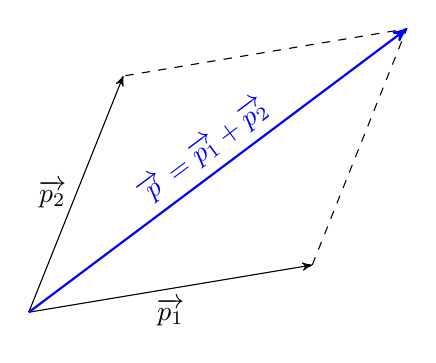
\begin{tikzpicture}[scale=1.2]
		\draw[->] (0,0) -- (3,0.5) node[midway,below]{$\overrightarrow{p_1}$};
		\draw[->] (0,0) -- (1,2.5) node[midway,left]{$\overrightarrow{p_2}$};
		\draw[dashed] (3,0.5) -- (4,3) -- (1,2.5);
		\draw[thick, ->, blue] (0,0) -- (4,3) node[midway,above,rotate=36.87]{$\overrightarrow{p} = \overrightarrow{p_1} + \overrightarrow{p_2}$};
		\end{tikzpicture}
	\end{minipage}
	\begin{minipage}[b]{0.45\textwidth}
		\centering
		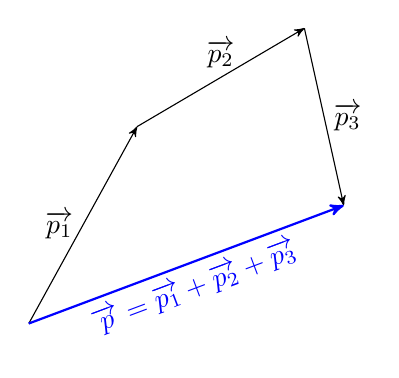
\begin{tikzpicture}[scale=1.25]
		\draw[->] (0,0) -- (1.1,2) node[midway,left]{$\overrightarrow{p_1}$};
		\draw[->] (1.1,2) -- (2.8,3) node[midway,above]{$\overrightarrow{p_2}$};
		\draw[->] (2.8,3) -- (3.2,1.2) node[midway,right]{$\overrightarrow{p_3}$};
		\draw[thick, ->, blue] (0,0) -- (3.2,1.2) node[midway,below,rotate=20.556]{$\overrightarrow{p} = \overrightarrow{p_1} + \overrightarrow{p_2} + \overrightarrow{p_3}$};
		\end{tikzpicture}
	\end{minipage}
\end{figure}

\example{A river flows from south to north with a speed of $2.0 \mps$ and the speed of a boat with respect to the water flow is $5.0 \mps$. (a) Suppose the boat leaves the west bank heading due east, what is the resultant velocity of the boat? (b) If the boat is to reach the exact opposite bank across the river, what is the resultant velocity and in what direction should the boat be headed?}

\sol vector diagrams for resultant velocity of the boat is illustrated below

\begin{figure}[ht]
	\centering
	\begin{minipage}[b]{0.45\textwidth}
		\centering
		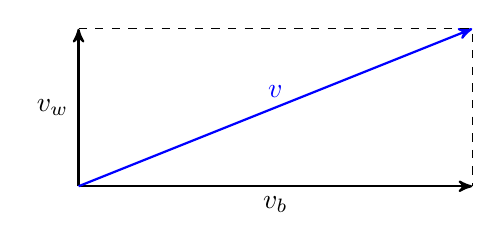
\begin{tikzpicture}
		\draw[thick,->] (0,0) -- (0,2) node[midway,left]{$v_w$};
		\draw[thick,->] (0,0) -- (5,0) node[midway,below]{$v_b$};
		\draw[thick,blue,->] (0,0) -- (5,2) node[midway,above]{$v$};
		\draw[dashed] (0,2) -- (5,2) -- (5,0);
		\end{tikzpicture}
		
		\vspace*{20pt}
		
		(a) boat heading due south
	\end{minipage}
	\begin{minipage}[b]{0.45\textwidth}
		\centering
		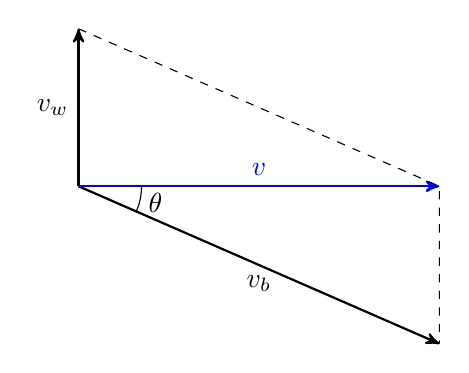
\begin{tikzpicture}
		\draw[thick,->] (0,0) -- (0,2) node[midway,left]{$v_w$};
		\draw[thick,->] (0,0) -- (4.583,-2) node[midway,below]{$v_b$};
		\draw[thick,blue,->] (0,0) -- (4.583,0) node[midway,above]{$v$};
		\draw[dashed] (0,2) -- (4.583,0) -- (4.583,-2);
		\draw (0.8,0) arc(0:-23.58:0.8);
		\node at (-12:1) {$\theta$};
		\end{tikzpicture}
		
		(b) boat aiming at exact opposite bank
	\end{minipage}
\end{figure}

\begin{compactitem}
	\item[(a)] magnitude of resultant velocity: $v = \sqrt{v_b^2 + v_w^2} = \sqrt{5.0^2 +2.0^2} \approx 5.4 \mps$
	
	in this case, the boat reaches the opposite bank in shortest time but will drift downstream
	
	\item[(b)] magnitude of resultant velocity: $v = \sqrt{v_b^2 + v_w^2} = \sqrt{5.0^2 -2.0^2} \approx 4.6 \mps$
	
	in this case, the boat reaches the opposite bank in shortest distance
	
	but the boat is headed slightly upstream: $\theta = \sin^{-1} \frac{v_w}{v_b} = \sin^{-1}\frac{2.0}{5.0} \approx 24^\circ$ \eoe
\end{compactitem}



\subsubsection{resolving vectors}

one can also resolve a single vector into two (or more) components
\footnote{This depends on the number of dimensions of space we are working with.}

\begin{wrapfigure}{R}{0.36\textwidth}
	\vspace{-18pt}
	\begin{center}
		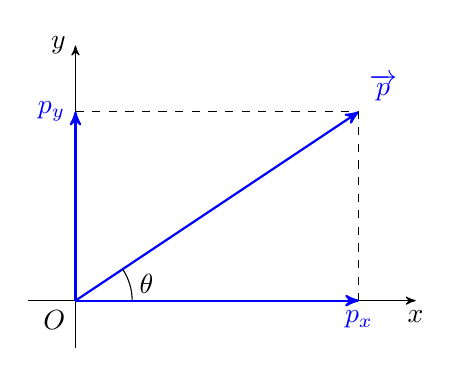
\begin{tikzpicture}[scale=1.2]
		\draw[->] (-.5,0) -- (3.6,0) node[below]{$x$};
		\draw[->] (0,-.5) -- (0,2.7) node[left]{$y$};
		\draw[thick, ->, blue] (0,0) node[below left]{\textcolor{black}{$O$}} -- (3,2) node[above right]{$\overrightarrow{p}$};
		\draw[dashed] (0,2) -- (3,2) -- (3,0);
		\draw[thick, ->, blue] (0,0) -- (0,2) node[left]{$p_y$};
		\draw[thick, ->, blue] (0,0) -- (3,0) node[below]{$p_x$};
		\draw (0:0.6) arc [radius=0.6, start angle=0, end angle= 33.7] node[midway,right]{$\theta$};
		\end{tikzpicture}
	\end{center}
	\vspace{-25pt}
\end{wrapfigure}

let's place a general 2D vector $\overrightarrow{p}$ in Cartesian coordinates

vector $\overrightarrow{p}$ can be split into two perpendicular components

\titem a horizontal component $p_x$

\titem a vertical component $p_y$

if $\overrightarrow{p}$ forms an angle $\theta$ to the $x$-axis, then:

{
	\centering
	
	$p_x = p \cos \theta, \quad p_y = p \sin \theta$
	
	$p = |\overrightarrow{p}| = \sqrt{p^2_x + p^2_y}, \quad\tan \theta = \frac{p_y}{p_x}$
	
}


\example{A force of 3.0 N towards east and a force of 2.0 N towards 30$^\circ$ north of east act on an object. Find the magnitude and the direction of the resultant force.}


\sol suppose an arrow of length 1 cm represents a force of 1 N

one can draw a \emph{scale diagram} with a ruler and a protractor as shown

\begin{figure}[ht]
	\centering
	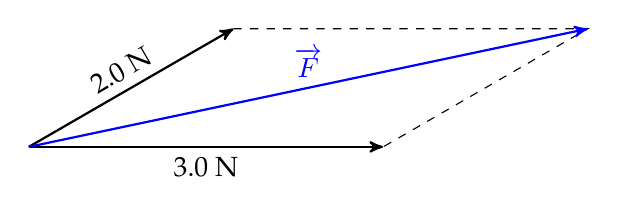
\begin{tikzpicture}[scale = 1.5]
	\draw[thick,->] (0,0) -- (3,0) node[midway,below]{3.0 N};
	\draw[thick,->] (0,0) -- ++ (30:2) node[midway,above,rotate=30]{2.0 N};
	\draw[dashed] (30:2) --++ (3,0) --++ (-150:2);
	\draw[thick,blue,->] (0,0) -- (4.732,1) node[midway, above]{$\overrightarrow{F}$};
	\end{tikzpicture}
\end{figure}

one can find length of the resultant vector is about 4.8 cm

also it forms an angle of about 12$^\circ$ to the 3.0 N force

so resultant force is of 4.8 N acting towards 12$^\circ$ north of east

alternatively, one can find components of the resultant as the sum of individual components

{
	\centering
	
	$F_x = 3.0 + 2.0 \cos 30^\circ \approx 4.73 \text{ N}, \quad F_y = 2.0\sin30^\circ = 1.0 \text{ N}$
	
}

magnitude and direction of the resultant can then be found from its components

{
	\centering
	
	$F = \sqrt{F_x^2 + F_y^2} = \sqrt{4.73^2 + 1.0^2} \approx 4.84 \text{ N}, \theta = \tan^{-1}\frac{F_y}{F_x} = \tan^{-1}\frac{1.0}{4.73} \approx 11.9^\circ$
	
}

this of course agrees with scale diagram method, but resolving gives more precise results \eoe

\begin{wrapfigure}{r}{0.5\textwidth}
	\vspace*{-10pt}
	\centering
	\begin{tikzpicture}[scale=1.1]
	\draw[thick] (0,0) -- (30:5) -- ++(0,-2.5) -- cycle;
	\draw[thick] (0.8,0) arc(0:30:0.8);
	\node at (15:1) {$\theta$};
	\draw[thick] (30:2.5) -- ++(120:1) -- ++(30:1) -- ++(-60:1);
	\draw[thick] (-1,0) -- (5,0);
	\draw[thick,->] (2.348,1.933) --++ (0,-1.6) node[right,pos=0.7]{$W$};
	\draw[thick,blue,->] (2.348,1.933) --++ (210:0.8) node[left]{$W_\parallelslant$};
	\draw[thick,blue,->] (2.348,1.933) --++ (-60:1.38564) node[right]{$W_\perp$};;
	\draw[dashed] (2.348,1.933) ++ (210:0.8) --++ (-60:1.38564) --++ (30:0.8) ;
	\end{tikzpicture}
	\vspace*{-16pt}
\end{wrapfigure}


\example{A box of weight $W=20.0 \text{ N}$ is resting on an inclined slope at 30$^\circ$ to the horizontal. Find the components of weight parallel to the slope and normal to the slope.}\label{ex:comp-of-W}

\sol the vector diagram is shown

component of weight parallel to slope: $W_\parallelslant = W\sin\theta = 20.0\times \sin30^\circ = 10.0 \text{ N}$

component of weight normal to slope: $W_\perp = W\cos\theta = 20.0\times \cos30^\circ \approx 17.3 \text{ N}$ \eoe


 
\subsection{uncertainties}
 
physics is a practical science, any law of physics must be evidenced by experimental facts

any meaningful physical quantity is measured either directly or indirectly

but repeated readings may not give a consistent value, instead they show a \emph{spread} of data

\keypoint{uncertainty} gives the \emph{range} of values in which \emph{true value} of the measurement is asserted to lie

measurement of a particular quantity is usually reported as $x \pm \Delta x$, where reported value $x$ is the average of repeated readings, and $\Delta x$ is its uncertainty

\subsubsection{absolute uncertainty}

$\Delta x$ measures the size of the range of values where true value probably lies

therefore $\Delta x$ is called the \keypoint{absolute uncertainty}\index{uncertainty!absolute uncertainty}

\cmt absolute uncertainty $\Delta x$ carries the same unit as quantity $x$

\cmt absolute uncertainty can be worked out from \emph{range} of readings

range of a data set ${x_1, x_2, x_3, \cdots}$ is the difference between greatest and smallest value

absolute uncertainty is given by: $\boxed{\Delta x = \frac{1}{2}\left(x_\tmax-x_\tmin\right)}$

\cmt absolute uncertainty is usually kept to one significant figure only
\footnote{In some cases where the uncertainty of a quantity is not stated explicitly, the uncertainty is indicated by the number of significant figures in the stated value. If the height of a person is measured to be 1.75 m, this means the first two digits (1 and 7) are certain, while the last digit (5) is uncertain.
	
When you add or subtract numbers, the number of significant figures is determined by the location of the decimal place. For example, $1.11+\underline{4.2}+0.563=5.873$, the result should be written as $5.9$. When you multiply or divided numbers, the result can have no more significant figures than the term with the fewest significant figures. For example, $1.35\times462\times\underline{0.27} = 168.399$, the result should be written as 170.

However, in AS \& A-Level physics, apart from the problems regarding uncertainties, it is allowed to give one more significant figure that what is required. So in other sections of my notes where we do not keep track of the uncertainties, I could be a bit sloppy with the issue of significant figures when numerical values are worked out.}

since $\Delta x$ indicates where the readings start to get problematic

measured quantity $x$ is kept to the same decimal place as $\Delta x$

for example, if value for the speed of an athlete is found to be $v=(8.16\pm0.27)\mps$, the result, to an appropriate number of significant figures, should be kept as: $v=(8.2\pm0.3) \mps$.



\subsubsection{fractional \& percentage uncertainty}

ratio of absolute uncertainty to reported value, i.e., $\frac{\Delta x}{x}$, gives the \keypoint{fractional uncertainty}

recording this ratio as a percentage number, this is known as the \keypoint{percentage uncertainty}\index{uncertainty!percentage uncertainty}

\cmt fractional and percentage uncertainty have no unit

\cmt $\frac{\Delta x}{x}$ gives relative measure of spread of data, so it is also called the relative uncertainty

\example{A students measures the diameter of a cylindrical bottle with a vernier calliper. The measurements are taken from several different positions and along different directions. The readings she obtained are: 4.351 cm, 4.387 cm, 4.382 cm, 4.372 cm, 4.363 cm. What is the percentage uncertainty of her measurements?}

\sol average value: $d = \frac{1}{5}(4.351+4.387+4.382+4.372+4.363) = 4.371 \text{ cm}$

absolute uncertainty: $\Delta d = \frac{1}{2}\left(d_\tmax-d_\tmin\right) = \frac{1}{2}(4.387-4.351) = 0.036 \text{ cm}$

result of measurement should be recorded as: $ d = 4.37 \pm 0.04 \text{ cm}$

percentage uncertainty: $\frac{\Delta d}{d} = \frac{0.036}{4.371} \approx 0.082\%$   \eoe




\subsubsection{propagation of uncertainties}\index{uncertainty!propagation}

in many situations, the quantity that we want to find cannot be measured directly

the quantity of interest has to be computed from other quantities

uncertainty of this calculated quantity would depend on two things:

\titem uncertainties of the raw data from which it is calculated,

\titem how calculated quantity is related to those original quantities

\vspace*{\baselineskip}

suppose quantities $A$ and $B$ are two measurables with uncertainty $\Delta A$ and $\Delta B$ 

$X$ is a quantity to be computed by taking their sum, difference, product or quotient

to evaluate uncertainty in $X$, we estimate the worst scenario, i.e., the greatest deviation from its reported value

\subsubsection*{addition: $S=A+B$}

$S_\tmax = A_\tmax + B_\tmax = (A + \Delta A) + (B + \Delta B) = (A+B) + (\Delta A + \Delta B)= S + (\Delta A + \Delta B) \RA \boxed{\Delta S = \Delta A + \Delta B}$

\subsubsection*{subtraction: $D=A-B$}

$D_\tmax = A_\tmax - B_\tmin = (A + \Delta A) - (B - \Delta B) = (A-B) + (\Delta A + \Delta B)= D + (\Delta A + \Delta B) \RA \boxed{\Delta D = \Delta A + \Delta B}$

\subsubsection*{multiplication: $P=AB$}

$P_\tmax = A_\tmax B_\tmax = (A + \Delta A)(B + \Delta B) = AB + B\Delta A + A\Delta B + \Delta A \Delta B \RA \Delta P =  B\Delta A + A\Delta B + \Delta A \Delta B$

divide both sides by $P=AB$, we get
\begin{equation*}
\frac{\Delta P}{P} = \frac{\Delta A}{A} + \frac{\Delta B}{B} + \frac{\Delta A}{A}\cdot\frac{\Delta B}{B} \RA \boxed{\frac{\Delta P}{P} = \frac{\Delta A}{A} + \frac{\Delta B}{B}}
\end{equation*}

percentage uncertainty of a measurable is usually a few percent, so $\frac{\Delta A}{A}\cdot\frac{\Delta B}{B} \approx 0$

so this piece is dropped from the last expression

\subsubsection*{division: $Q=\frac{A}{B}$}

one can show that $\boxed{\frac{\Delta Q}{Q} = \frac{\Delta A}{A} + \frac{\Delta B}{B}}$

the derivation is left as an exercise for the reader

\subsubsection*{power \& roots: $Q=A^l B^m C^n\cdots$}

percentage uncertainty in $Q$ is: $\frac{\Delta Q}{Q} = l\frac{\Delta A}{A} + m\frac{\Delta B}{B} + n\frac{\Delta C}{C} +\cdots$

this can be thought of as a generalization for multiplication and division operations

the proof is also left as an exercise to the reader

\subsubsection*{brief summary}

\begin{ilight}
	-- for addition and subtraction, \emph{absolute uncertainties} add up
	
	-- for multiplication, division and powers, \emph{percentage uncertainties} add up
	
\end{ilight}

\cmt notice that uncertainties always add

\example{The resistance of a resistor is measured in an experiment. The current through the resistor is $1.8\pm0.1$ A and the potential difference across is $7.5\pm 0.2$ V. What is the resistance of the resistor and its uncertainty?}

value of resistance: $R=\frac{V}{I} = \frac{7.5}{1.8} \approx 4.17  \text{ }\Omega$

percentage uncertainty in resistance: $\frac{\Delta R}{R} = \frac{\Delta V}{V} + \frac{\Delta I}{I} = \frac{0.2}{7.5} + \frac{0.1}{1.8} \approx 8.2 \%$

absolute uncertainty in resistance: $\Delta R = 8.2\% \times 4.17 \approx 0.34 \text{ }\Omega$

so we find resistance of the resistor: $R = 4.2 \pm 0.3  \text{ }\Omega$ \eoe

\example{The density of a liquid is found by measuring its mass and its volume. The following is a summary of the measurements: $\text{mass of empty beaker} = (20\pm1)\text{g}$, $\text{mass of beaker and liquid} = (100\pm1)\text{g}$,  and $\text{volume of liquid} = (10.0\pm0.5)\text{cm}^3$. What is the density of this liquid and the uncertainty in this value?}

\sol mass of liquid: $m = m_2 - m_1 = 100 -20 = 80 \text{ g}$

uncertainty in mass: $\Delta m = \Delta m_2 + \Delta m_1 = 1 + 1 = 2 \text{ g}$

density of liquid: $\rho = \frac{m}{V} = \frac{80}{10.0} = 8.00 \text{ g cm}^{-3}$

percentage uncertainty in density: $\frac{\Delta \rho}{\rho} = \frac{\Delta m}{m} + \frac{\Delta V}{V} = \frac{2}{80} + \frac{0.5}{10.0} = 7.5 \%$

absolute uncertainty in density: $\Delta \rho = 7.5\% \times 8.00 = 0.60 \text{ g cm}^{-3}$

so density of this liquid is recorded as: $\rho = 8.0 \pm 0.6 \text{ g cm}^{-3}$ \eoe

\example{The period of simple pendulum is given by $T=2\pi\sqrt{\frac{L}{g}}$. In an experiment, the length of string is measured to be $L=100.0\pm0.5$ cm, and the time taken for 10 full oscillations is $t=20.0\pm 0.2$ s. What is the value for acceleration of free fall $g$ and its uncertainty?}

\sol period of one oscillation: $T = \frac{1}{10}t = 2.00 \pm 0.02 \text{ s}$

let's rearrange $T=2\pi\sqrt{\frac{L}{g}}$ into $g = \frac{4\pi^2L}{T^2}$

acceleration of free fall: $g = \frac{4\pi^2 \times 100.0}{2.00^2} \approx 987 \text{ cm s}^{-2}$

\eqyskip percentage uncertainty: $\frac{\Delta g}{g} = \frac{\Delta L}{L} + 2\frac{\Delta T}{T} = \frac{0.5}{100.0} + 2\times\frac{0.02}{2.00} = 2.5\%$ \footnote{Starting from the formula $T=2\pi\sqrt{\frac{L}{g}}$, it is attempting to write $\frac{\Delta T}{T} = \frac{1}{2}\frac{\Delta L}{L} + \frac{1}{2}\frac{\Delta g}{g}$. But this would mean that $T$ is a calculated quantity whose uncertainty is determined by the uncertainty in $L$ and the uncertainty in $g$, which is incorrect. The right way to do it is to rearrange the formula so that calculated quantity of interest is made the subject of the working equation, the propagation of uncertainties then becomes explicit.}

absolute uncertainty: $\Delta g = 2.5\% \times 987 \approx 24.7 \text{ cm s}^{-2}$

so result of this measurement is: $ g = 990 \pm 20 \text{ cm s}^{-2}$ \eoe




\subsection{measurement errors}

difference between the measured value and the true value is called \keypoint{error}

total error is usually a combination of two components: systematic error and random error

\subsubsection{systematic \& random errors}

\begin{ilight}
	\keypoint{systematic errors} cause the readings to be greater or smaller than the true value by the same amount\index{systematic error}
\end{ilight}

\cmt faulty equipments, biased observers, calibration errors could produce systematic errors

examples of systematic errors include:

\titem a vernier calliper does not read zero when fully closed, this introduces \keypoint{zero error}

\titem one always reads a measuring cylinder from a higher angle, this introduces \keypoint{parallax error}

\titem spring of force meter becomes weaker over time, so force meter always gives overestimates

\cmt systematic errors can be reduced by using better equipments or methods

\titem one can check for zero error before taking readings with a micrometer

\titem one can \emph{calibrate} a balance with a known mass before using it to measure mass of an object



\begin{ilight}
	\keypoint{random errors} cause the readings to fluctuate above or below the actual value\index{random error}
\end{ilight}


\cmt deviations caused by random error are unpredictable

\cmt insensitive equipments, lack of observer precision, changes in environment, imprecise definitions could produce random errors

examples of causes of random errors include:

\titem \keypoint{human reaction errors} when measuring a time quantity on a stop-watch

\titem electronic noise due to thermal vibrations of atoms when measuring an electric current

\titem when measuring length of a crack, different people could pick different end points

\cmt random errors can be reduced by averaging the results from repeated measurements

for example, diameter of a sphere can be measured along different directions and averaged

\cmt random errors can also be reduced by using better equipment and better technique

for example, time for an object to fall can be measured with a light gate, instead of a stopwatch

\begin{wrapfigure}{r}{0.5\textwidth}
	\centering
	\vspace*{-15pt}
	\begin{tikzpicture}[xscale=1,yscale=0.9]
	\draw[<->] (0,5) node[left]{$I$} -- (0,0) -- (6,0) node[below]{$V$};
	\node[blue] at (1.5,0.4) {$\times$};
	\node[blue] at (2.5,1.6) {$\times$};
	\node[blue] at (3.6,2.3) {$\times$};
	\node[blue] at (4.8,3.4) {$\times$};
	\node[blue] at (5.6,4.7) {$\times$};
	\draw[thick,red] (0.5,-0.4) --++ (5.5,5.2);
	\end{tikzpicture}
	\vspace*{-15pt}
\end{wrapfigure}

\example{An experiment is carried out to measure the resistance of a metallic resistor, which is known to be constant throughout the experiment. A set of readings for voltage $V$ across the resistor and the corresponding current $I$ are obtained. A graph of $I$ against $V$ is plotted as shown. What can you say about the errors of the experiment?}

\sol one can first draw a \emph{best fit line} to see the distribution of data points

constant resistance means $I$ should be directly proportional to $V$

so the best fit should be a straight line through the origin

but the best fit does not pass through origin, so there exists systematic error

also data points scatter above and below the best fit, so random errors are present \eoe


\subsubsection{accuracy \& precision}

to analyse the result of an experiment, two important aspects are accuracy and precision

\begin{ilight}
	measurement is said to be \keypoint{accurate} if the result is close to the true value\index{accuracy}
\end{ilight}

\begin{ilight}
	measurement is said to be \keypoint{precise} if repeated readings are close to each other\index{precision}
\end{ilight}

\begin{figure}[htp]
	\centering
	\begin{minipage}{0.32\textwidth}
		\centering
		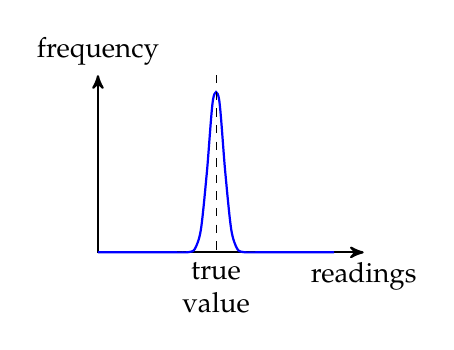
\begin{tikzpicture}[scale = .75]
		\draw [thick, <->] (4.5,0) node[below]{readings} -- (0,0) --(0,3) node[above]{frequency};
		\draw [thick,blue,domain=0:4,samples=40,smooth,variable=\x] plot (\x, {2.8*exp(-30*(\x-2)^2)});
		\draw[dashed] (2,3) -- (2,0) node[below,align=center,execute at begin node=\setlength{\baselineskip}{1.2em}]{true\\value};
		\end{tikzpicture}
		
		(a) precise and accurate
	\end{minipage}\hfil
	\begin{minipage}{0.32\textwidth}
		\centering
		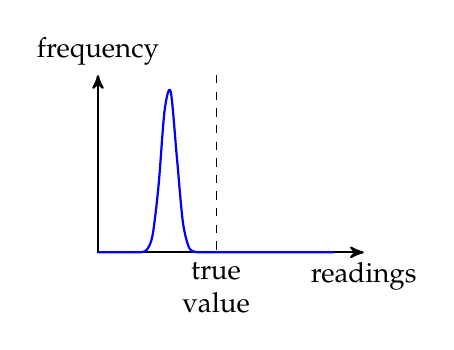
\begin{tikzpicture}[scale = .75]
		\draw [thick, <->] (4.5,0) node[below]{readings} -- (0,0) --(0,3) node[above]{frequency};
		\draw [thick,blue,domain=0:4,samples=40,smooth,variable=\x] plot (\x, {2.8*exp(-30*(\x-1.2)^2)});
		\draw[dashed] (2,3) -- (2,0) node[below,align=center,execute at begin node=\setlength{\baselineskip}{1.2em}]{true\\value};
		\end{tikzpicture}
		
		(b) precise but not accurate
	\end{minipage}\hfil
	\begin{minipage}{0.32\textwidth}
		\centering
		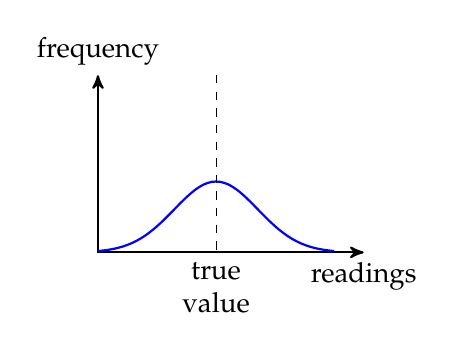
\begin{tikzpicture}[scale = .75]
		\draw [thick, <->] (4.5,0) node[below]{readings} -- (0,0) --(0,3) node[above]{frequency};
		\draw [thick,blue,domain=0:4,samples=30,smooth,variable=\x] plot (\x, {1.2*exp(-1*(\x-2)^2)});
		\draw[dashed] (2,3) -- (2,0) node[below,align=center,execute at begin node=\setlength{\baselineskip}{1.2em}]{true\\value};
		\end{tikzpicture}
		
		(c) accurate but not precise
	\end{minipage}
	
	\caption*{distribution of readings with different precision and accuracy}
\end{figure}

\cmt accuracy of a measurement is closely related to systematic errors

large systematic errors mean the results must be inaccurate

\cmt precision of a measurement is closely related to random errors

large random errors cause repeated readings to spread, so the result must be imprecise

\cmt precision is usually indicated by the percentage uncertainty of the measurement

similarly, precision is also indicated by the number of significant figures in a measurement

for example, metre rule has a precision of 0.1 cm, while micrometer has a precision of 0.001 cm


\example{The value for the acceleration of free fall is determined in an experiment. The result is reported to be $g=14\pm5 \mpss$. Is this result accurate? Is it precise?}

\sol true value for $g$ is around $9.8\mpss$

stated value is not close to the true value, so the result is not accurate

percentage uncertainty in this result is $\frac{5}{14}\approx 36\%$, which is quite large

so the result is not precise either \eoe



\ifthenelse{\includequestions=1}{
	
\subsection{end-of-chapter questions}

\subsubsection*{SI units}

\question{What are the SI base units of (a) density, (b) pressure, (c) energy, (d) electric charge?}

\question{For a substance of mass $m$, the heat energy $Q$ needed to change its temperature by $\Delta T$ is given by: $Q = cm\Delta T$. Find the SI base units of the constant $c$.}

\subsubsection*{dimensional analysis}

\question{The resistive force $F$ on a metal ball falling at low speeds in water is given by the equation $F = krv$, where $r$ is the radius of the metal ball, $v$ is its speed and $k$ is a constant.
	Find the base units of $k$ in the SI system.}

\question{The speed of sound in air can be given by $c=\sqrt{\frac{\gamma p}{\rho}}$, where $p$ is the pressure of the air and $\rho$ is the air density. Show that $\gamma$ is unit free.}

\question{The effective power output from a wind turbine is given by the equation $P = \frac{1}{2} \eta \rho A v^n$, where $\rho$ is the air density, $A$ is the area of the turbine blades, and $v$ is the wind speed. Given that $\eta$ is a constant with no units, what is the value of $n$?}

\subsubsection*{vector algebra}

\question{An aircraft, which has a speed of $35 \mps$ in still air, is flying from south to north at a speed of $32 \mps$ with respect to a stationary observer on the ground. Find the magnitude and the possible directions of wind velocity.}

\question{Three forces of 5.0 N, 12 N and 13 N act at one point on an object. The angles at which the forces act can vary. What is the maximum and the minimum resultant force?}

\subsubsection*{propagation of uncertainties}

\question{A thermometer can measure to a precision of $0.5 ^\circ$C , what is the temperature rise from $20.0 ^\circ$C to $50.0 ^\circ$C and its uncertainty?}

\question{The radius of a sphere is measured to be $5.0$ cm with an uncertainty of 1\%. What is the volume of this sphere and the uncertainty? (Volume of a sphere is given by: $V=\frac{4}{3}\pi R^3$.)}

\question{The power radiated from a star of radius $R$ and surface temperature $T$ is given by the formula: $P = 4\pi \sigma R^2 T^4$, where $\sigma$ is the Stefan–Boltzmann constant known to have the value of $5.67\times10^{-8} \text{ W m}^{-2} \text{ K}^{-4}$. If the sun is measured to have a surface temperature of $5800 \pm 200 \text{ K}$ and a diameter of $(1.40\pm0.03)\times10^9 \text{ m}$. (a) Find the radiation power $P$ of the sun and its absolute uncertainty. (b) Suggest which measurement has a larger effect on the uncertainty in $P$.}




}{}
\section{Measurements}

\subsection{uncertainties}

physics is a practical science, any law of physics must be evidenced by experimental facts

any meaningful physical quantity is measured either directly or indirectly

but repeated readings may not give a consistent value, instead they show a \emph{spread} of data

\keypoint{uncertainty} gives the \emph{range} of values in which \emph{true value} of the measurement is asserted to lie

measurement of a particular quantity is usually reported as $x \pm \Delta x$, where reported value $x$ is the average of repeated readings, and $\Delta x$ is its uncertainty

\subsubsection{absolute uncertainty}

$\Delta x$ measures the size of the range of values where true value probably lies

therefore $\Delta x$ is called the \keypoint{absolute uncertainty}\index{uncertainty!absolute uncertainty}

\cmt absolute uncertainty $\Delta x$ carries the same unit as quantity $x$

\cmt absolute uncertainty can be worked out from \emph{range} of readings

range of a data set ${x_1, x_2, x_3, \cdots}$ is the difference between greatest and smallest value

absolute uncertainty is given by: $\boxed{\Delta x = \frac{1}{2}\left(x_\tmax-x_\tmin\right)}$

\cmt absolute uncertainty is usually kept to one significant figure only
\footnote{In some cases where the uncertainty of a quantity is not stated explicitly, the uncertainty is indicated by the number of significant figures in the stated value. If the height of a person is measured to be 1.75 m, this means the first two digits (1 and 7) are certain, while the last digit (5) is uncertain.
	
	When you add or subtract numbers, the number of significant figures is determined by the location of the decimal place. For example, $1.11+\underline{4.2}+0.563=5.873$, the result should be written as $5.9$. When you multiply or divided numbers, the result can have no more significant figures than the term with the fewest significant figures. For example, $1.35\times462\times\underline{0.27} = 168.399$, the result should be written as 170.
	
	However, in AS \& A-Level physics, apart from the problems regarding uncertainties, it is allowed to give one more significant figure that what is required. So in other sections of my notes where we do not keep track of the uncertainties, I could be a bit sloppy with the issue of significant figures when numerical values are worked out.}

since $\Delta x$ indicates where the readings start to get problematic

measured quantity $x$ is kept to the same decimal place as $\Delta x$

for example, if value for the speed of an athlete is found to be $v=(8.16\pm0.27)\mps$, the result, to an appropriate number of significant figures, should be kept as: $v=(8.2\pm0.3) \mps$.



\subsubsection{fractional \& percentage uncertainty}

ratio of absolute uncertainty to reported value, i.e., $\frac{\Delta x}{x}$, gives the \keypoint{fractional uncertainty}

recording this ratio as a percentage number, this is known as the \keypoint{percentage uncertainty}\index{uncertainty!percentage uncertainty}

\cmt fractional and percentage uncertainty have no unit

\cmt $\frac{\Delta x}{x}$ gives relative measure of spread of data, so it is also called the relative uncertainty

\example{A students measures the diameter of a cylindrical bottle with a vernier calliper. The measurements are taken from several different positions and along different directions. The readings she obtained are: 4.351 cm, 4.387 cm, 4.382 cm, 4.372 cm, 4.363 cm. What is the percentage uncertainty of her measurements?}

\sol average value: $d = \frac{1}{5}(4.351+4.387+4.382+4.372+4.363) = 4.371 \text{ cm}$

absolute uncertainty: $\Delta d = \frac{1}{2}\left(d_\tmax-d_\tmin\right) = \frac{1}{2}(4.387-4.351) = 0.036 \text{ cm}$

result of measurement should be recorded as: $ d = 4.37 \pm 0.04 \text{ cm}$

percentage uncertainty: $\frac{\Delta d}{d} = \frac{0.036}{4.371} \approx 0.082\%$   \eoe




\subsubsection{propagation of uncertainties}\index{uncertainty!propagation}

in many situations, the quantity that we want to find cannot be measured directly

the quantity of interest has to be computed from other quantities

uncertainty of this calculated quantity would depend on two things:

\titem uncertainties of the raw data from which it is calculated,

\titem how calculated quantity is related to those original quantities

\vspace*{\baselineskip}

suppose quantities $A$ and $B$ are two measurables with uncertainty $\Delta A$ and $\Delta B$ 

$X$ is a quantity to be computed by taking their sum, difference, product or quotient

to evaluate uncertainty in $X$, we estimate the worst scenario, i.e., the greatest deviation from its reported value

\subsubsection*{addition: $S=A+B$}

$S_\tmax = A_\tmax + B_\tmax = (A + \Delta A) + (B + \Delta B) = (A+B) + (\Delta A + \Delta B)= S + (\Delta A + \Delta B) \RA \boxed{\Delta S = \Delta A + \Delta B}$

\subsubsection*{subtraction: $D=A-B$}

$D_\tmax = A_\tmax - B_\tmin = (A + \Delta A) - (B - \Delta B) = (A-B) + (\Delta A + \Delta B)= D + (\Delta A + \Delta B) \RA \boxed{\Delta D = \Delta A + \Delta B}$

\subsubsection*{multiplication: $P=AB$}

$P_\tmax = A_\tmax B_\tmax = (A + \Delta A)(B + \Delta B) = AB + B\Delta A + A\Delta B + \Delta A \Delta B \RA \Delta P =  B\Delta A + A\Delta B + \Delta A \Delta B$

divide both sides by $P=AB$, we get
\begin{equation*}
\frac{\Delta P}{P} = \frac{\Delta A}{A} + \frac{\Delta B}{B} + \frac{\Delta A}{A}\cdot\frac{\Delta B}{B} \RA \boxed{\frac{\Delta P}{P} = \frac{\Delta A}{A} + \frac{\Delta B}{B}}
\end{equation*}

percentage uncertainty of a measurable is usually a few percent, so $\frac{\Delta A}{A}\cdot\frac{\Delta B}{B} \approx 0$

so this piece is dropped from the last expression

\subsubsection*{division: $Q=\frac{A}{B}$}

one can show that $\boxed{\frac{\Delta Q}{Q} = \frac{\Delta A}{A} + \frac{\Delta B}{B}}$

the derivation is left as an exercise for the reader

\subsubsection*{power \& roots: $Q=A^l B^m C^n\cdots$}

percentage uncertainty in $Q$ is: $\frac{\Delta Q}{Q} = l\frac{\Delta A}{A} + m\frac{\Delta B}{B} + n\frac{\Delta C}{C} +\cdots$

this can be thought of as a generalization for multiplication and division operations

the proof is also left as an exercise to the reader

\subsubsection*{brief summary}

\begin{ilight}
	-- for addition and subtraction, \emph{absolute uncertainties} add up
	
	-- for multiplication, division and powers, \emph{percentage uncertainties} add up
	
\end{ilight}

\cmt notice that uncertainties always add

\example{The resistance of a resistor is measured in an experiment. The current through the resistor is $1.8\pm0.1$ A and the potential difference across is $7.5\pm 0.2$ V. What is the resistance of the resistor and its uncertainty?}

value of resistance: $R=\frac{V}{I} = \frac{7.5}{1.8} \approx 4.17  \text{ }\Omega$

percentage uncertainty in resistance: $\frac{\Delta R}{R} = \frac{\Delta V}{V} + \frac{\Delta I}{I} = \frac{0.2}{7.5} + \frac{0.1}{1.8} \approx 8.2 \%$

absolute uncertainty in resistance: $\Delta R = 8.2\% \times 4.17 \approx 0.34 \text{ }\Omega$

so we find resistance of the resistor: $R = 4.2 \pm 0.3  \text{ }\Omega$ \eoe

\example{The density of a liquid is found by measuring its mass and its volume. The following is a summary of the measurements: $\text{mass of empty beaker} = (20\pm1)\text{g}$, $\text{mass of beaker and liquid} = (100\pm1)\text{g}$,  and $\text{volume of liquid} = (10.0\pm0.5)\text{cm}^3$. What is the density of this liquid and the uncertainty in this value?}

\sol mass of liquid: $m = m_2 - m_1 = 100 -20 = 80 \text{ g}$

uncertainty in mass: $\Delta m = \Delta m_2 + \Delta m_1 = 1 + 1 = 2 \text{ g}$

density of liquid: $\rho = \frac{m}{V} = \frac{80}{10.0} = 8.00 \text{ g cm}^{-3}$

percentage uncertainty in density: $\frac{\Delta \rho}{\rho} = \frac{\Delta m}{m} + \frac{\Delta V}{V} = \frac{2}{80} + \frac{0.5}{10.0} = 7.5 \%$

absolute uncertainty in density: $\Delta \rho = 7.5\% \times 8.00 = 0.60 \text{ g cm}^{-3}$

so density of this liquid is recorded as: $\rho = 8.0 \pm 0.6 \text{ g cm}^{-3}$ \eoe

\example{The period of simple pendulum is given by $T=2\pi\sqrt{\frac{L}{g}}$. In an experiment, the length of string is measured to be $L=100.0\pm0.5$ cm, and the time taken for 10 full oscillations is $t=20.0\pm 0.2$ s. What is the value for acceleration of free fall $g$ and its uncertainty?}

\sol period of one oscillation: $T = \frac{1}{10}t = 2.00 \pm 0.02 \text{ s}$

let's rearrange $T=2\pi\sqrt{\frac{L}{g}}$ into $g = \frac{4\pi^2L}{T^2}$

acceleration of free fall: $g = \frac{4\pi^2 \times 100.0}{2.00^2} \approx 987 \text{ cm s}^{-2}$

\eqyskip percentage uncertainty: $\frac{\Delta g}{g} = \frac{\Delta L}{L} + 2\frac{\Delta T}{T} = \frac{0.5}{100.0} + 2\times\frac{0.02}{2.00} = 2.5\%$ \footnote{Starting from the formula $T=2\pi\sqrt{\frac{L}{g}}$, it is attempting to write $\frac{\Delta T}{T} = \frac{1}{2}\frac{\Delta L}{L} + \frac{1}{2}\frac{\Delta g}{g}$. But this would mean that $T$ is a calculated quantity whose uncertainty is determined by the uncertainty in $L$ and the uncertainty in $g$, which is incorrect. The right way to do it is to rearrange the formula so that calculated quantity of interest is made the subject of the working equation, the propagation of uncertainties then becomes explicit.}

absolute uncertainty: $\Delta g = 2.5\% \times 987 \approx 24.7 \text{ cm s}^{-2}$

so result of this measurement is: $ g = 990 \pm 20 \text{ cm s}^{-2}$ \eoe




\subsection{errors of measurement}

difference between the measured value and the true value is called \keypoint{error}

total error is usually a combination of two components: systematic error and random error

\subsubsection{systematic \& random errors}

\begin{ilight}
	\keypoint{systematic errors} cause the readings to be greater or smaller than the true value by the same amount\index{systematic error}
\end{ilight}

\cmt faulty equipments, biased observers, calibration errors could produce systematic errors

examples of systematic errors include:

\titem a vernier calliper does not read zero when fully closed, this introduces \keypoint{zero error}

\titem one always reads a measuring cylinder from a higher angle, this introduces \keypoint{parallax error}

\titem spring of force meter becomes weaker over time, so force meter always gives overestimates

\cmt systematic errors can be reduced by using better equipments or methods

\titem one can check for zero error before taking readings with a micrometer

\titem one can \emph{calibrate} a balance with a known mass before using it to measure mass of an object



\begin{ilight}
	\keypoint{random errors} cause the readings to fluctuate above or below the actual value\index{random error}
\end{ilight}


\cmt deviations caused by random error are unpredictable

\cmt insensitive equipments, lack of observer precision, changes in environment, imprecise definitions could produce random errors

examples of causes of random errors include:

\titem \keypoint{human reaction errors} when measuring a time quantity on a stop-watch

\titem electronic noise due to thermal vibrations of atoms when measuring an electric current

\titem when measuring length of a crack, different people could pick different end points

\cmt random errors can be reduced by averaging the results from repeated measurements

for example, diameter of a sphere can be measured along different directions and averaged

\cmt random errors can also be reduced by using better equipment and better technique

for example, time for an object to fall can be measured with a light gate, instead of a stopwatch

\begin{wrapfigure}{r}{0.5\textwidth}
	\centering
	\vspace*{-15pt}
	\begin{tikzpicture}[xscale=1,yscale=0.9]
	\draw[<->] (0,5) node[left]{$I$} -- (0,0) -- (6,0) node[below]{$V$};
	\node[blue] at (1.5,0.4) {$\times$};
	\node[blue] at (2.5,1.6) {$\times$};
	\node[blue] at (3.6,2.3) {$\times$};
	\node[blue] at (4.8,3.4) {$\times$};
	\node[blue] at (5.6,4.7) {$\times$};
	\draw[thick,red] (0.5,-0.4) --++ (5.5,5.2);
	\end{tikzpicture}
	\vspace*{-15pt}
\end{wrapfigure}

\example{An experiment is carried out to measure the resistance of a metallic resistor, which is known to be constant throughout the experiment. A set of readings for voltage $V$ across the resistor and the corresponding current $I$ are obtained. A graph of $I$ against $V$ is plotted as shown. What can you say about the errors of the experiment?}

\sol one can first draw a \emph{best fit line} to see the distribution of data points

constant resistance means $I$ should be directly proportional to $V$

so the best fit should be a straight line through the origin

but the best fit does not pass through origin, so there exists systematic error

also data points scatter above and below the best fit, so random errors are present \eoe


\subsubsection{accuracy \& precision}

to analyse the result of an experiment, two important aspects are accuracy and precision

\begin{ilight}
	measurement is said to be \keypoint{accurate} if the result is close to the true value\index{accuracy}
\end{ilight}

\begin{ilight}
	measurement is said to be \keypoint{precise} if repeated readings are close to each other\index{precision}
\end{ilight}

\begin{figure}[htp]
	\centering
	\begin{minipage}{0.32\textwidth}
		\centering
		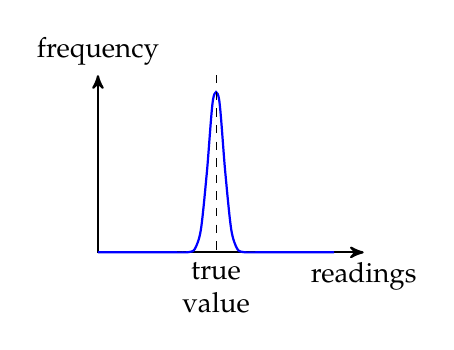
\begin{tikzpicture}[scale = .75]
		\draw [thick, <->] (4.5,0) node[below]{readings} -- (0,0) --(0,3) node[above]{frequency};
		\draw [thick,blue,domain=0:4,samples=40,smooth,variable=\x] plot (\x, {2.8*exp(-30*(\x-2)^2)});
		\draw[dashed] (2,3) -- (2,0) node[below,align=center,execute at begin node=\setlength{\baselineskip}{1.2em}]{true\\value};
		\end{tikzpicture}
		
		(a) precise and accurate
	\end{minipage}\hfil
	\begin{minipage}{0.32\textwidth}
		\centering
		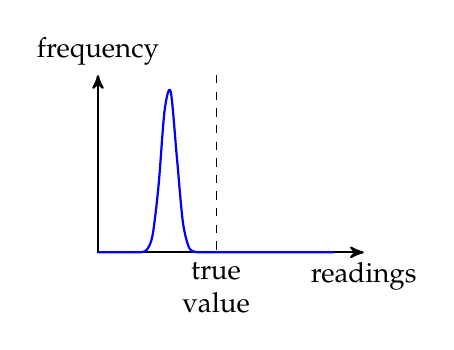
\begin{tikzpicture}[scale = .75]
		\draw [thick, <->] (4.5,0) node[below]{readings} -- (0,0) --(0,3) node[above]{frequency};
		\draw [thick,blue,domain=0:4,samples=40,smooth,variable=\x] plot (\x, {2.8*exp(-30*(\x-1.2)^2)});
		\draw[dashed] (2,3) -- (2,0) node[below,align=center,execute at begin node=\setlength{\baselineskip}{1.2em}]{true\\value};
		\end{tikzpicture}
		
		(b) precise but not accurate
	\end{minipage}\hfil
	\begin{minipage}{0.32\textwidth}
		\centering
		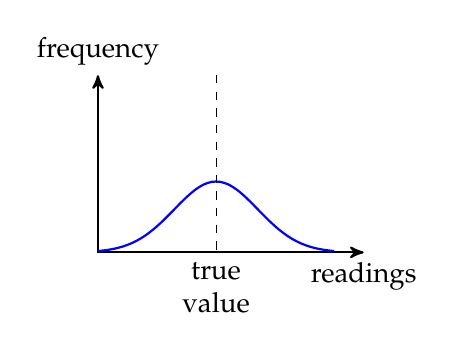
\begin{tikzpicture}[scale = .75]
		\draw [thick, <->] (4.5,0) node[below]{readings} -- (0,0) --(0,3) node[above]{frequency};
		\draw [thick,blue,domain=0:4,samples=30,smooth,variable=\x] plot (\x, {1.2*exp(-1*(\x-2)^2)});
		\draw[dashed] (2,3) -- (2,0) node[below,align=center,execute at begin node=\setlength{\baselineskip}{1.2em}]{true\\value};
		\end{tikzpicture}
		
		(c) accurate but not precise
	\end{minipage}
	
	\caption*{distribution of readings with different precision and accuracy}
\end{figure}

\cmt accuracy of a measurement is closely related to systematic errors

large systematic errors mean the results must be inaccurate

\cmt precision of a measurement is closely related to random errors

large random errors cause repeated readings to spread, so the result must be imprecise

\cmt precision is usually indicated by the percentage uncertainty of the measurement

similarly, precision is also indicated by the number of significant figures in a measurement

for example, metre rule has a precision of 0.1 cm, while micrometer has a precision of 0.001 cm


\example{The value for the acceleration of free fall is determined in an experiment. The result is reported to be $g=14\pm5 \mpss$. Is this result accurate? Is it precise?}

\sol true value for $g$ is around $9.8\mpss$

stated value is not close to the true value, so the result is not accurate

percentage uncertainty in this result is $\frac{5}{14}\approx 36\%$, which is quite large

so the result is not precise either \eoe





\ifthenelse{\includequestions=1}{
	
	\subsection{end-of-chapter questions}
		
	\subsubsection*{propagation of uncertainties}
	
	\question{A thermometer can measure to a precision of $0.5 ^\circ$C , what is the temperature rise from $20.0 ^\circ$C to $50.0 ^\circ$C and its uncertainty?}
	
	\question{The radius of a sphere is measured to be $5.0$ cm with an uncertainty of 1\%. What is the volume of this sphere and the uncertainty? (Volume of a sphere is given by: $V=\frac{4}{3}\pi R^3$.)}
	
	\question{The power radiated from a star of radius $R$ and surface temperature $T$ is given by the formula: $P = 4\pi \sigma R^2 T^4$, where $\sigma$ is the Stefan–Boltzmann constant known to have the value of $5.67\times10^{-8} \text{ W m}^{-2} \text{ K}^{-4}$. If the sun is measured to have a surface temperature of $5800 \pm 200 \text{ K}$ and a diameter of $(1.40\pm0.03)\times10^9 \text{ m}$. (a) Find the radiation power $P$ of the sun and its absolute uncertainty. (b) Suggest which measurement has a larger effect on the uncertainty in $P$.}
	
	
	
	
}{}
\section{Kinematics}

Kinematics is the study of motion. In this chapter, we define three useful kinematic quantities, displacement, velocity and acceleration, and use these terms to discuss the motion of an object.

\subsection{kinematic quantities}

\subsubsection{displacement \& distance}

in everyday language, we talk about the \keypoint{distance} travelled by an object, which usually refers to the length travelled by an object without considering in what direction it moves

to fully describe position of an object, we also need specify where it moves

\begin{ilight}
	we define \keypoint{displacement} as the distance moved by an object in a specific direction\index{displacement}
\end{ilight}

\cmt displacement and distance are measured in metres, or any reasonable length units

\cmt displacement is a vector quantity, while distance is a scalar

\cmt displacement is the \emph{straight-line} distance pointing from starting point towards end point

even if actual path taken is curved, displacement is always the straight-line distance

\begin{figure}[!ht]
	\centering
	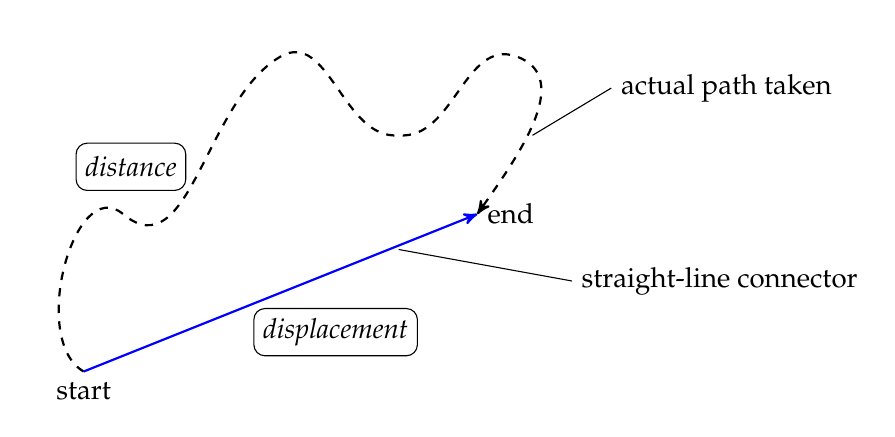
\begin{tikzpicture}[scale=1]
%	\draw[step=0.5] (0,0) grid (5,5);
	 \draw[thick, dashed,->] (0,0) node[below]{start} [out=150, in=140] to (0.5,2) [out=-40, in=210] to (2.5,4) [out=30, in=185] to (4,3) [out=-5, in=160] to (5.5,4) [out=-20, in=55] to (5,2) node[right]{end};
	 \draw[thick, blue, ->] (0,0) -- (5,2) ;
	 \node[note] at (0.6,2.6) {distance};
	 \node[note] at (3.2,0.5) {displacement};
	 \draw (5.7,3) --++ (1,0.6) node[right] {actual path taken};
	 \draw (4,1.55) --++ (2.2,-0.4) node[right] {straight-line connector};
	\end{tikzpicture}
	
	\caption*{difference between displacement and distance}
\end{figure}


\example{An athlete is running around a circular track of radius 60 m. When he completes one lap, what is the distance moved out? What about his displacement?}

\sol distance moved is the perimeter of the circle: $s = 2\pi r = 2\pi\times 60 \approx 380 \text{ m}$

athlete returns to same starting point after one lap, so displacement is zero \eoe

\begin{wrapfigure}{r}{0.4\textwidth}
%	\vspace*{-12pt}
	\centering
	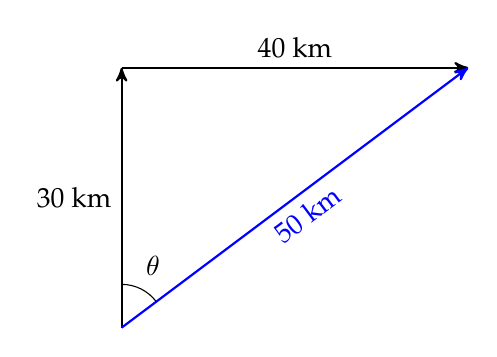
\begin{tikzpicture}[scale=1.1]
	\draw[thick,->] (0,0) -- (0,3) node[midway, left]{30 km};
	\draw[thick,->] (0,3) -- (4,3) node[midway, above]{40 km};
	\draw[thick,blue,->] (0,0) -- (4,3) node[midway, below, rotate=36.89]{50 km};
	\draw (0,0.5) arc(90:36.89:0.5);
	\node at (63:0.8) {$\theta$};
	\end{tikzpicture}
	\vspace*{-16pt}
\end{wrapfigure}

\example{A ship travels 30 km north, takes a right, and then travels 40 km east to reach its destination. Compare the distance and the displacement travelled.}

\sol sum of all lengths gives distance: $30+40 = 70 \text{ km}$

displacement vector is shown on the graph

$\text{magnitude of displacement} = \sqrt{30^2 + 40^2} = 50 \text{ km}$

it is at an angle of $\theta = \tan^{-1}\frac{40}{30} \approx 53^\circ$ east of north \eoe



\subsubsection{velocity \& speed}

displacement of a moving object may change with respect to time

an object is moving fast if it has a large change in displacement during a given time interval

\begin{ilight}
	change in displacement per unit time is called the \keypoint{velocity} of the object\index{velocity}: $\boxed{v=\frac{\Delta s}{\Delta t}}$
\end{ilight}

\cmt SI unit of measurement for velocity: $[v]= \mps$

\cmt velocity is a vector quantity

this follows from the fact that displacement is a vector quantity

\cmt for \emph{linear} motion, one shall pick a specific direction as the positive direction

then a negative velocity implies motion in the opposite direction

\cmt it is also common to use \keypoint{speed} to describe how fast an object moves

speed is defined as the change of the distance travelled per unit time

velocity can be thought as speed in a particular direction

\cmt defining equation $v=\frac{\Delta s}{\Delta t}$ gives the \emph{average} value for velocity or speed over an interval $\Delta t$

more precisely: $\boxed{\text{average velocity} = \frac{\text{total displacement}}{\text{time taken}}}$, and $\boxed{\text{average speed} = \frac{\text{total distance}}{\text{time taken}}}$

\eqyskip this should be distinguished from the notion of \emph{instantaneous velocity}

instantaneous velocity is defined as the rate of change in displacement at a particular instant

if we take a very short interval $\Delta t$, as $\Delta t \to 0$, average velocity tends to instantaneous velocity

this is expressed in a compact differential form: $v = \lim_{\Delta t \to 0} \frac{\Delta s}{\Delta t} \ra \boxed{v=\frac{\dd s}{\dd t}} $

\example{A cyclist travels a distance of 3.0 km in 20 minutes. She rests for 15 minutes. She then covers a further distance of 5.1 km in a time of 40 minutes. Calculate the average speed of the cyclist in m s$^{-1}$: (a) during the first 20 minutes of the journey, (b) for the whole journey.}

\sol for the first 20 minutes: $ v = \frac{3.0\times10^3}{20 \times 60} = 2.5 \mps$

\eqyskip for whole journey: $v = \frac{(3.0+0+5.1)\times10^3}{(20+15+40)\times60} = 1.8 \mps $ \eoe

\example{A man walks along a straight road for a distance of 800 m in 5.0 minutes. He then turns around, and walks along the same road for a distance of 280 m in 3.0 minutes. What is the average speed and the average velocity of this man during the 8.0 minutes?}

\sol $\text{total distance travelled} = 800 + 280 = 1080 \text{m}$, so average speed: $v = \frac{1080}{8.0\times60} = 2.25 \mps$

\eqyskip  $\text{change of displacement} = 800 + (-280) = 520 \text{m}$, so average velocity: $v = \frac{520}{8.0\times60} \approx 1.08 \mps$ \eoe

\example{A maglev train travels at an average speed of $60\mps$ from the city centre to the airport, and at $40\mps$ on its return journey over the same distance. What is the average speed of the round-trip? What about the average velocity?}

\sol suppose the distance between airport and city centre is $S$

average speed: $v = \frac{2S}{t_1 + t_2} = \frac{2S}{\frac{S}{60} + \frac{S}{40}} = 48 \mps$

for a round-trip, train returns to same staring position

change in displacement is zero, so average velocity is zero \eoe



\subsubsection{acceleration}

velocity of a moving object may change as well, i.e., objects can speed up or slow down

\begin{ilight}
	change in velocity per unit time is defined as the \keypoint{acceleration}\index{acceleration}: $\boxed{a = \frac{\Delta v}{\Delta t}}$
\end{ilight}

\cmt unit of measurement for acceleration: $[a]= \mpss$

\cmt acceleration is a vector quantity, it has both magnitude and direction

this is because of vector nature of velocity, change in velocity must also have direction

\cmt for \emph{linear} motion, one usually pick direction of initial velocity as positive direction

$a>0$ would imply acceleration in the normal sense, i.e., motion with an increasing speed

$a<0$ would imply deceleration, i.e., motion with a decreasing speed

\cmt when velocity changes, it could be change in magnitude or/and change in direction
\footnote{Acceleration of an object can be considered as the combination of two components. One component is known as the \emph{normal} acceleration or the \emph{centripetal} acceleration, which is at right angle to the velocity and is responsible for the change in direction of motion. The other component is called the \emph{tangential} acceleration, which is parallel to the direction of motion and causes change in magnitude of object's velocity. You will learn more about these in further mechanics.}

for example, for an object moving along a curved path, its velocity is constantly changing direction, so it must have a non-zero acceleration

no acceleration would imply no change in speed and no change in direction of motion

\cmt defining equation $a = \frac{\Delta v}{\Delta t}$ gives average acceleration over time interval $\Delta t$

we can likewise introduce \emph{instantaneous acceleration} as the rate of change in velocity

taking the limit where the time interval $\Delta t \to 0$. we have: $a = \lim_{\Delta t \to 0} \frac{\Delta v}{\Delta t} \ra \boxed{a=\frac{\dd v}{\dd t}} $

\example{A ball hits a barrier at right angles with a speed of $15 \mps$. It makes contact with the barrier for 30 ms and then rebounds with a speed of $12 \mps$. What is the average acceleration during the time of contact?}

\sol note that direction of velocity changed during rebound, so $\Delta v = 15 - (-12) = 27 \mps$

average acceleration: $a = \frac{\Delta v}{\Delta t} = \frac{27}{30 \times 10^{-3}} = 900 \mpss$ \eoe



\subsection{motion graphs}

how one physical quantity changes with another quantity can be visually shown on a \emph{graph}

changes in displacement, velocity or acceleration over time can be shown on \emph{motion graphs}\index{motion graphs}

as we will see, $s$-$t$ graph, $v$-$t$ graph and $a$-$t$ graphs are closely interrelated to one another

\subsubsection{displacement-time graphs}

a displacement-time graph shows an object's position at any given time

\cmt gradient of tangent gives rate of change in displacement

but this is instantaneous velocity, which can be given by $v = \frac{\dd s}{\dd t}$, so we have:

{
	\centering
	
	\eqyskip$ \boxed{\text{velocity} = \text{gradient of $s$-$t$ graph}} $
	
}

\newpage


\example{Describing the motion from the displacement-time graph shown.}

\begin{wrapfigure}{L}{0.36\textwidth}
	\vspace{-24pt}
	\begin{center}
		\begin{tikzpicture}[xscale=1.1,yscale=0.95]
		\draw[<->] (0,3.2)node[left]{s} -- (0,0) -- (4.2,0)node[below]{$t$};
		\draw[blue, thick] plot [smooth] coordinates {(0,0) (.5,.2) (1,.8) (1.5,2.0) (2,2.5) (2.5,2.7) (3.0,2.8) (4,2.8)};
		\node at (.8,1) {$A$};
		\node at (2,2.8) {$B$};
		\node at (3.5,3) {$C$};
		\end{tikzpicture}
	\end{center}
	\vspace{-27pt}
\end{wrapfigure}

	stage $A$: gradient of the graph is increasing, showing that the object is speeding up
		
	stage $B$: gradient starts to decrease, so the object gradually slows down
		
	stage $C$: curve becomes horizontal, gradient becomes zero, means that the object eventually comes to a stop \eoe
	
\begin{wrapfigure}{r}{0.45\textwidth}
	\vspace*{-12pt}
	\centering
	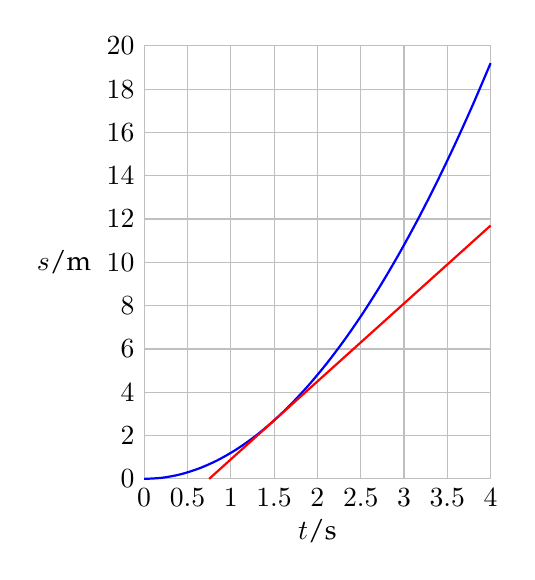
\begin{tikzpicture}[scale=1.1]
		\draw[gray!50,step=0.5] (0,0) grid (4,5);
		\draw[thick, blue,smooth, samples=20, domain=0:4] plot (\x, 0.3*\x*\x);
		\foreach \x in {0,0.5,1,1.5,2,2.5,3,3.5,4} \node[below] at (\x,0){$\x$};
		\foreach \y in {0,2,...,20} \node[left] at (0,\y/4) {$\y$};
		\node at (2,-0.6) {$t$/s};
		\node[left] at (-0.5,2.5) {$s$/m};
		\draw[thick,red] (0.75,0) -- (4,2.925);
	\end{tikzpicture}
	\vspace*{-10pt}
\end{wrapfigure}

\example{The diagram shows the displacement-time graph for a vehicle travelling along a straight road. Use the graph to find, (a) the average velocity during the first 4.0 s of the motion, (b) the velocity of the vehicle \emph{at} time $t=1.5$ s.}

\sol during first 4.0 s, average velocity is

{
	\centering
	
	$ v = \frac{\Delta s}{\Delta t} = \frac{19.2}{4.0} \approx 4.8 \mps$
	
}

to find velocity at $t=1.5$ s, a tangent is drawn

gradient of tangent gives instantaneous velocity:

{
	\centering
	
	$ v = \frac{11.6 - 0}{4.0-0.75} \approx 3.6 \mps $
	
}

\vspace*{-\baselineskip} \eoe

\subsubsection{velocity-time graphs}

a velocity-time graph shows the velocity of a moving object at any instant

\cmt since the rate of change of velocity gives the acceleration, so
\begin{equation*}
\boxed{\text{acceleration} = \text{gradient of $v$-$t$ graph}}
\end{equation*}

\cmt $v$-$t$ graph also gives information about the change in displacement
\begin{equation*}
\boxed{\text{change in displacement} = \text{area under $v$-$t$ graph}}
\end{equation*}

in very short time interval $\Delta t_i$, change in velocity is small so $v(t_i)\approx\text{constant}$ during this time

displacement moved out $\Delta s_i \approx v(t_i) \Delta t_i$, which corresponds to area of a thin rectangle

sum of all these small $\Delta s_i$'s gives total change in displacement over a period of time

now consider the limit where each of the time interval $\Delta t_i \to 0$

total area of these rectangles approximates area bounded by the $v$-$t$ curve and time axis
\footnote{Mathematically, integration is the inverse operation of taking derivatives. By definition $v=\frac{\dd s}{\dd t}$, then it follows naturally that $\Delta s = \int v\dd t$. While the derivative of a given function gives the gradient of tangent at each point on its graph, integrating a function gives the signed area bounded by the graph. The reader may find the formal treatment of this relationship in any calculus textbook.}

\begin{figure}[!ht]
	\noindent\centering
	\begin{minipage}{0.32\linewidth}
	\centering
	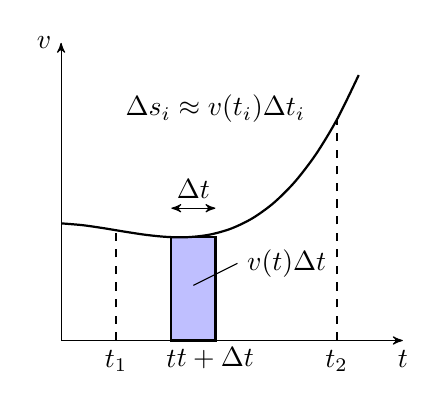
\begin{tikzpicture}[scale=1.4]
	\draw[thick,fill=blue!25] (1.5,0) rectangle (1.9,0.9375);
	\draw (1.7,0.5) -- (2.1,0.7) node[right]{$v(t)\Delta t$};
	\draw[<->] (1.5,1.2) -- (1.9,1.2) node[midway,above]{$\Delta t$};
	\draw[<->] (0.5,2.7) node[left]{$v$} -- (0.5,0) -- (3.6,0) node[below]{$t$};
	\draw [thick,domain=0.5:3.2,samples=15,smooth,variable=\x] plot (\x,{\x*(\x-1)*(\x-2)/6+1});
	\draw[thick,dashed] (1,0) node[below]{$t_1$} -- (1,1);
	\draw[thick,dashed] (3,0) node[below]{$t_2$} -- (3,2);
	\node[below] at (1.5,0) {$t$};
	\node[below] at (1.9,0.02) {$t+\Delta t$};
	\node at (1.9,2.1){$\Delta s_i \approx v(t_i)\Delta t_i$};
	\end{tikzpicture}
	(a) displacement $\Delta s$
	
	in short interval $\Delta t$
	\end{minipage}\hfill
	\begin{minipage}{0.34\linewidth}
		\centering
		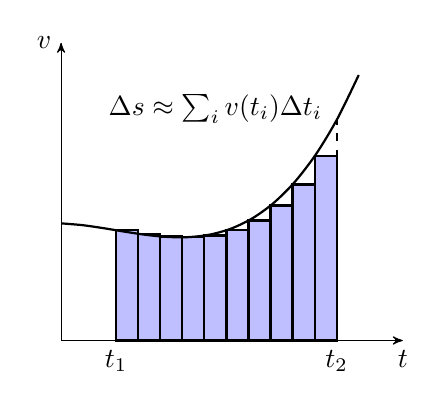
\begin{tikzpicture}[scale=1.4]
		\foreach \x in {1.0,1.2,1.4,...,2.8}
		{ \draw[thick,fill=blue!25] (\x,0) rectangle (\x+.2,{\x*(\x-1)*(\x-2)/6+1});
			}
		\draw[thick,dashed] (1,0) node[below]{$t_1$} -- (1,1);
		\draw[thick,dashed] (3,0) node[below]{$t_2$} -- (3,2);
		\draw[<->] (0.5,2.7) node[left]{$v$} -- (0.5,0) -- (3.6,0) node[below]{$t$};
		\draw [thick,domain=0.5:3.2,samples=15,smooth,variable=\x] plot (\x,{\x*(\x-1)*(\x-2)/6+1});
		\node at (1.9,2.1){$\Delta s \approx \sum_i v(t_i)\Delta t_i$};
		\end{tikzpicture}
		(b) total displacement estimated	
		
		by summing the many $\Delta s_i$'s
	\end{minipage}\hfill
	\begin{minipage}{0.32\linewidth}
		\centering
		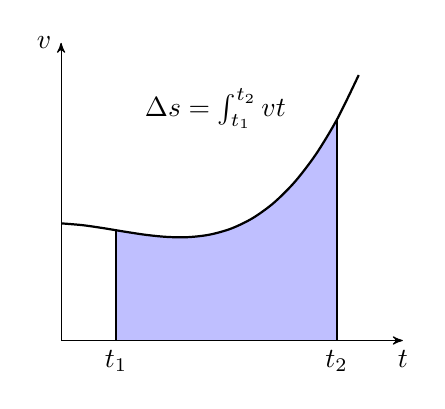
\begin{tikzpicture}[scale=1.4]
		\fill[fill=blue!25] (1,0) -- plot[domain=1:3,samples=15,smooth,variable=\x] (\x,{\x*(\x-1)*(\x-2)/6+1}) -- (3,0) -- cycle;
		\draw[thick] (1,0) node[below]{$t_1$} -- (1,1);
		\draw[thick] (3,0) node[below]{$t_2$} -- (3,2);
		\draw[<->] (0.5,2.7) node[left]{$v$} -- (0.5,0) -- (3.6,0) node[below]{$t$};
		\draw [thick,domain=0.5:3.2,samples=15,smooth,variable=\x] plot (\x,{\x*(\x-1)*(\x-2)/6+1});
		\node at (1.9,2.1){$\Delta s = \int_{t_1}^{t_2} v \dd t$};
		\end{tikzpicture}
		(c) total displacement as
		
		area under $v$-$t$ graph
	\end{minipage}
	\caption*{calculating change in displacement by finding the area under velocity-time graph}\label{fig:area_of_vt}
\end{figure}

\begin{wrapfigure}{r}{0.45\textwidth}
	\vspace*{0pt}
	\centering
	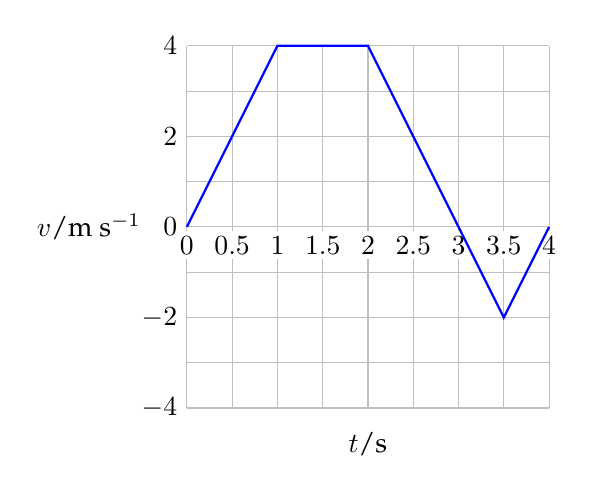
\begin{tikzpicture}[scale=1.15]
	\draw[gray!50,step=0.5] (0,-2) grid (4,2);
	\foreach \x in {0,0.5,1,1.5,2,2.5,3,3.5,4} {
	\draw[white,fill] (\x-0.1,-0.35) rectangle (\x+0.1,-0.05);
	\node[below] at (\x,0){$\x$};
	}
	\foreach \y in {-4,-2,0,2,4} \node[left] at (0,\y/2) {$\y$};
	\draw[blue,thick] (0,0) -- (1,2) -- (2,2) -- (3.5,-1) -- (4,0);
	\node at (2,-2.4) {$t$/s};
	\node[left] at (-0.4,0) {$v$/m s$^{-1}$};
	\end{tikzpicture}
	\vspace*{-16pt}
\end{wrapfigure}


\example{The velocity of a toy car is shown. For the journey shown on the graph, use the graph to find (a) the total distance travelled, and (b) the total displacement travelled.}

\sol distance is estimated using area under $v$-$t$ graph

0$\sim$3.0 s: $s_1 = \frac{1}{2}\times{1.0+3.0}\times4.0 = 8.0 \text{ m}$

3.0$\sim$4.0 s: $s_2 = \frac{1}{2}\times{1.0}\times2.0 = 1.0 \text{ m}$

$\text{total distance} = 8.0 + 1.0 = 9.0 \text{ m}$

$\text{total displacement} = (+8.0) + (-1.0) = 7.0 \text{ m}$ \eoe

\subsubsection{acceleration-time graphs}

one can similarly plot an acceleration-time graph to give the changes in acceleration

\cmt $a$-$t$ graphs can give information about changes in velocity

similar discussions lead to the following conclusion:\footnote{Using area under $a$-$t$ graph to find changes in velocity is not required in the AS-Level physics syllabus. I am putting this in the notes mainly for the completeness of the discussions on motion graphs.}
\begin{equation*}
\boxed{\text{change in velocity} = \text{area under $a$-$t$ graph}}
\end{equation*}

\newpage

relationships between displacement, velocity and acceleration graphs are summarised below

\begin{figure}[!ht]
	\centering
	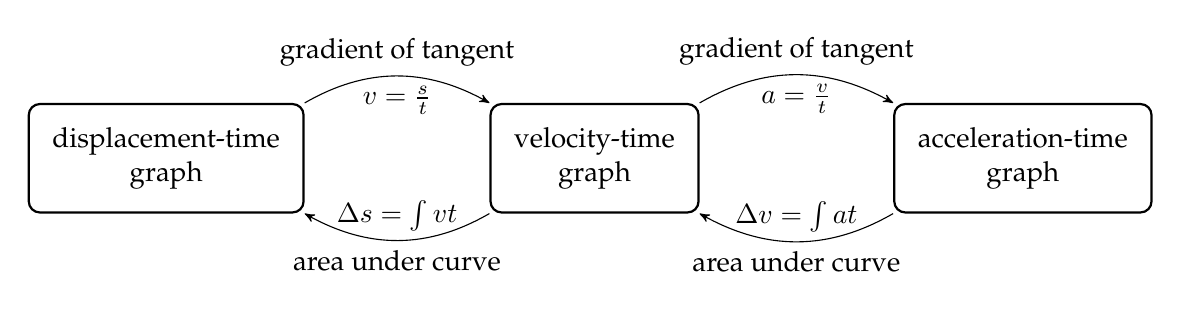
\begin{tikzpicture}[force/.style={align=center,execute at begin node=\setlength{\baselineskip}{1.2em},draw,thick,rounded corners,inner sep=.3cm},scale=0.85]
	
	\node [force] (displacement) at (0,0) {displacement-time\\ graph};
	\node [force] (velocity) at (6.4,0) {velocity-time\\graph};
	\node [force] (acceleration) at (12.8,0) {acceleration-time\\graph};
	
	\draw[->] (displacement.north east) to [bend left] node[midway,above]{gradient of tangent} node[midway,below]{$v=\frac{\dd s}{\dd t}$} (velocity.north west);
	\draw[<-] (displacement.south east) to [bend right] node[midway,below]{area under curve} node[midway,above]{$\Delta s=\int v\dd t$} (velocity.south west);
	\draw[->] (velocity.north east) to [bend left] node[midway,above]{gradient of tangent} node[midway,below]{$a=\frac{\dd v}{\dd t}$} (acceleration.north west);
	\draw[<-] (velocity.south east) to [bend right] node[midway,below]{area under curve} node[midway,above]{$\Delta v=\int a\dd t$} (acceleration.south west);
	\end{tikzpicture}
%	\caption*{relationships between motion graphs}
\end{figure}

\example{Given the displacement-time graph as shown, check yourself that this $s$-$t$ graph leads to the velocity-time graph and the acceleration-time graph shown.}

\begin{figure}[ht]
	\centering
	\begin{minipage}{0.3\textwidth}
		\centering
		\begin{tikzpicture}[xscale=0.6,yscale=0.9]
		\draw[<->] (0,2) node[left]{$s$} -- (0,0) -- (7,0) node[below]{$t$};
		\draw (0,0) -- (0,-2);
		\draw [thick,blue,domain=0:6.7,smooth] plot (\x, {1.6*sin(\x r)});
		\end{tikzpicture}
	\end{minipage}\hfil
	\begin{minipage}{0.3\textwidth}
		\centering
		\begin{tikzpicture}[xscale=0.6,yscale=0.9]
		\draw[<->] (0,2) node[left]{$v$} -- (0,0) -- (7,0) node[below]{$t$};
		\draw (0,0) -- (0,-2);
		\draw [thick,red,domain=0:6.7,smooth] plot (\x, {1.6*cos(\x r)});
		\end{tikzpicture}
	\end{minipage}\hfil
	\begin{minipage}{0.3\textwidth}
		\centering
		\begin{tikzpicture}[xscale=0.6,yscale=0.9]
		\draw[<->] (0,2) node[left]{$a$} -- (0,0) -- (7,0) node[below]{$t$};
		\draw (0,0) -- (0,-2);
		\draw [thick,red,domain=0:6.7,smooth] plot (\x, {-1.6*sin(\x r)});
		\end{tikzpicture}
	\end{minipage}
\end{figure}

\example{Given the velocity-time graph as shown, check yourself that this $v$-$t$ graph leads to the displacement-time graph as shown.}\label{ex-vgraph}

\begin{figure}[ht]
	\centering
	\begin{minipage}{0.45\textwidth}
		\centering
		\begin{tikzpicture}[xscale=0.8,yscale=1.1]
		\draw[<->] (0,3) node[left]{$v$} -- (0,0) -- (7,0) node[below]{$t$};
		\draw [thick,blue] (0,0) -- (2,2.5) -- (4,2.5) [out=-75,in=180] to (6,0);
		\draw[dashed] (2,0) -- (2,2.5)  (4,0) -- (4,2.5);
		\end{tikzpicture}
	\end{minipage}\hfil
	\begin{minipage}{0.45\textwidth}
		\centering
		\begin{tikzpicture}[xscale=0.8,yscale=1.1]
		\draw[<->] (0,3) node[left]{$s$} -- (0,0) -- (7,0) node[below]{$t$};
		\draw [thick,red,domain=0:2] plot (\x,0.2*\x*\x);
		\draw [thick,red] (2,0.8) -- (4,2.4);
		\draw [thick,red,domain=4:6] plot (\x,{2.4+0.8*(1-exp(-2.5*\x+2.5*4))/2.5});
		\draw[dashed] (2,0) -- (2,0.8)  (4,0) -- (4,2.4);
		\end{tikzpicture}
	\end{minipage}
\end{figure}





\subsection{linear motion with constant velocity}

let's look at the simplest kind of motion

that is, an object moving at constant speed in a straight line: $v=\text{constant}$

the equations of motion are straightforward:
\begin{equation}
	a=0 \qquad \boxed{s=vt}\footnote{It is implicitly assumed that the motion starts from the origin with respect to which displacement is defined. More generically, we should write: $s = s_0 + vt$, where $s_0$ is the initial displacement.}
\end{equation}

\begin{figure}[htp]
	\centering
	\begin{minipage}{0.32\textwidth}
		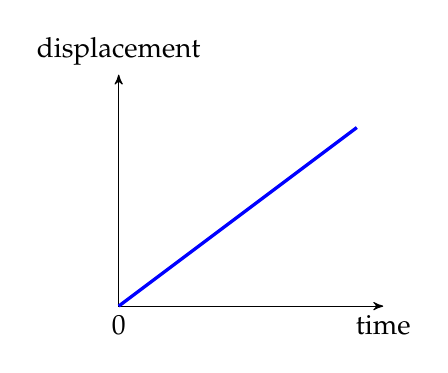
\begin{tikzpicture}[scale=0.84]
		\draw [<->] (0,3.5) node[above] {displacement} -- (0,0) node[below]{0} -- (4,0) node[below] {time};
		\draw[very thick,blue] (0,0) -- (3.6,2.7);
		\end{tikzpicture}
	\end{minipage}\hfill
	\begin{minipage}{0.32\textwidth}
		\begin{tikzpicture}[scale=0.84]
		\draw [<->] (0,3.5) node[above] {velocity} -- (0,2.5) node[left]{$v$} -- (0,0) node[below]{0} -- (4,0) node[below] {time};
		\draw[very thick,blue] (0,2.5) -- (3.6,2.5);
		\draw[dashed] (3,2.5) -- (3,0) node[below]{$t$};
		\end{tikzpicture}
	\end{minipage}\hfill
	\begin{minipage}{0.32\textwidth}
		\begin{tikzpicture}[scale=0.84]
		\draw [<->] (0,3.5) node[above] {acceleration} -- (0,0) node[below]{0} -- (4,0) node[below] {time};
		\draw[very thick,blue] (0,0.01) -- (3.6,0.01);
		\end{tikzpicture}
	\end{minipage}
	\caption*{motion graphs for linear motion at constant velocity}
\end{figure}



\subsection{linear motion with constant acceleration}

the second simplest type of motion is a linear motion with acceleration $a=\text{constant}$

\begin{figure}[htp]
	\centering
	\begin{minipage}{0.32\textwidth}
		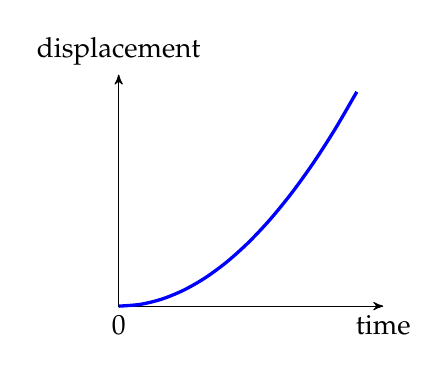
\begin{tikzpicture}[scale=0.84]
		\draw [<->] (0,3.5) node[above] {displacement} -- (0,0) node[below]{0} -- (4,0) node[below] {time};
		\draw [very thick,blue,domain=0:3.6,samples=12,smooth,variable=\x] plot (\x,{\x*\x/4});
		\end{tikzpicture}
	\end{minipage}\hfill
	\begin{minipage}{0.32\textwidth}
		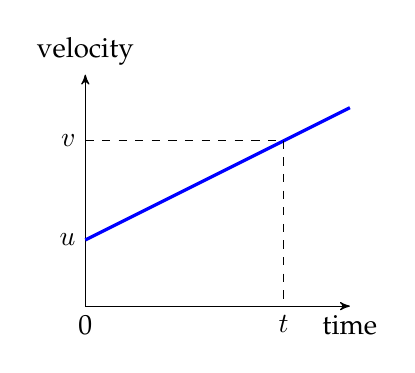
\begin{tikzpicture}[scale=0.84]
		\draw [<->] (0,3.5) node[above] {velocity} -- (0,1) node[left]{$u$} -- (0,0) node[below]{0} -- (4,0) node[below]{time};
		\draw[very thick,blue] (0,1) -- (4,3);
		\draw[dashed] (0,2.5) node[left]{$v$}  -- (3,2.5);
		\draw[dashed] (3,2.5) -- (3,0) node[below]{$t$};
		\end{tikzpicture}
	\end{minipage}\hfill
	\begin{minipage}{0.32\textwidth}
		\begin{tikzpicture}[scale=0.84]
		\draw [<->] (0,3.5) node[above] {acceleration} -- (0,2.5) node[left]{$a$} -- (0,0) node[below]{0} -- (4,0) node[below] {time};
		\draw[very thick,blue] (0,2.5) -- (3.6,2.5);
		\end{tikzpicture}
	\end{minipage}
	\caption*{motion graphs for linear motion at constant acceleration}\label{fig:const_a_graph}
\end{figure}

\subsubsection{equations of motion}

during a time interval $t$, suppose velocity changes from initial value $u$ to final value $v$

from the defining equation of acceleration $a=\frac{\Delta v}{\Delta t} = \frac{v-u}{t}$, we get
\begin{equation}\label{eqn:const_a_eq1}
\boxed{v=u+at}
\footnote{Proof with calculus: $\dd v = a \dd t \ra \Delta v = \int_u^v \dd v = \int_0^t a\dd t \ra v-u=at \ra v=u+at$}
\end{equation}

to find total displacement travelled, we compute the area under the $v$-$t$ graph
\begin{equation}\label{eqn:const_a_eq2}
	\boxed{s=\frac{1}{2}(u+v)t}
\end{equation}
for which we can interpret $\bar{v}=\frac{1}{2}(u+v)$ as the average velocity during that time

plug \eqref{eqn:const_a_eq1} into \eqref{eqn:const_a_eq2}, we find an expression for the displacement travelled in terms of $u$ and $a$:
\begin{equation}\label{eqn:const_a_eq3}
	\boxed{s = ut + \frac{1}{2}at^2}
	\footnote{Proof with calculus: $\dd s = v \dd t \ra \Delta s = \int_0^s \dd s = \int_0^t v\dd t \ra s = \int_0^t (u+at)\dd t = \big(ut+\frac{1}{2}at^2\big)\bigg|_0^t \ra s = ut + \frac{1}{2}at^2$}
	\footnote{Equation \eqref{eqn:const_a_eq3} assumes a zero initial displacement at $t=0$. If there is a non-zero initial displacement, one should write $s = s_0 + ut + \frac{1}{2}at^2$. Similar discussion applies to equation \eqref{eqn:const_a_eq2}.}
\end{equation}

this shows the displacement $s$ is a quadratic function in time $t$

this is consistent with the parabolic shape of the $s$-$t$ graph shown

we can also eliminate the time variable $t$ to derive one last equation

from \eqref{eqn:const_a_eq1} we have $t=\frac{v-u}{a}$, substitute this into \eqref{eqn:const_a_eq2}, we find
\begin{equation}\label{eqn:const_a_eq4}
	s=\frac{1}{2}(u+v)\times\frac{v-u}{a} \RA \boxed{2as = v^2 - u^2}
\end{equation}

\example{A car starts from rest and accelerates uniformly at 5.0\mpss for 6.0 s. (a) How fast is the car travelling at $t=8.0$ s? (b) What is the distance travelled by the car in this time?}

\solc\begin{equation*}
v=u+at \RA v = 0 + 5.0\times 6.0 = 30 \mps
\end{equation*}
\begin{equation*}
s=ut+\frac{1}{2}at^2 \RA s= 0+\frac{1}{2}\times5.0\times6.0^2 = 90 \text{ m} \teoe
\end{equation*}

\example{A car is travelling at 30\mps. A hazard appears in front of the car, and the driver takes immediate action to stop the car. When brakes are applied, deceleration of the car is 5.0\mpss. What is the braking distance?}

\solc\begin{equation*}
2as=v^2-u^2 \RA s = \frac{v^2-u^2}{2a} = \frac{0^2 - 30^2}{2\times(-5.0)} = 90 \text{ m} \teoe
\end{equation*}

\example{At the instant the traffic light turns green, a motorcycle waiting at the stop line starts with a constant acceleration of $2.0 \mpss$. At the same instant, a truck at a constant speed of $16 \mps$ overtakes and passes the motorcycle. How far beyond the stop line will the motorcycle overtake the truck?}

\sol suppose overtake occurs at time $t$ after motorcycle starts to accelerate

distance travelled by motorcycle: $s_m = u_mt + \frac{1}{2}at^2  \RA s_m = 0 + \frac{1}{2}\times 2.0 \times t^2$

distance travelled by truck: $s_t = v_t t \RA s_t = 16t$

overtake when $s_m = s_t \RA \frac{1}{2}\times 2.0 \times t^2 = 16 t \RA t=16 \text{ s}$

substitute $t$ into either $s_m$ or $s_t$, one finds distance travelled: $s = 256 \text{ m}$ \eoe




\subsubsection{free fall}\label{ch_freefall}

a typical example of uniformly accelerated motion is the free fall\index{free fall}

everything has the tendency to fall towards ground due to earth's gravity

in this section, we assume that effects of air resistance are negligible

acceleration of free fall is then a constant $a=g$, regardless of mass of falling object\footnote{The reason for this constant acceleration of free fall will be elaborated in $\S$\ref{ch_weight}.}

\cmt near surface of earth, value of acceleration of free fall: $g\approx9.81\mpss$

value of $g$ could be different on a different planet

\cmt for a freely-falling object released from rest, its velocity increases with time as
\begin{equation*}
	v=u+at = 0 + gt \RA v = gt
\end{equation*}

the distance it has fallen from the point of release is
\begin{equation*}
s=ut+\frac{1}{2} at^2 = 0\cdot t + \frac{1}{2}gt^2 \RA s=\frac{1}{2}gt^2
\end{equation*}

\example{An object is released from rest from a height of $h=24$ m and falls freely under gravity. Air resistance is negligible. (a) How long does it take to hit the ground? (b) What is its speed when hitting the ground?}

\solc\begin{equation*}
h = \frac{1}{2}gt^2 \RA t = \sqrt{\frac{2h}{g}} = \sqrt{\frac{2\times24}{9.81}} \approx 2.21 \text{ s}
\end{equation*}
\begin{equation*}
v = gt = 9.81 \times 2.21 \approx 21.7 \mps \teoe
\end{equation*}

\example{A photograph is taken for a small particle falling from rest. The photograph is taken at 0.400 s after the object is released. Since the particle is still moving when the photograph is being taken, the image is blurred. The blurred part is found to have a length of 20.8 cm. What is time of exposure for the photograph?}

\sol from $t=0$ to right before photo is taken: 

{
	\centering
	
	$s_1 = \frac{1}{2}gt_1^2 = \frac{1}{2}\times9.81\times0.400^2 \approx 0.785 \text{ m}$
	
}

from $t=0$ to right after photo has been taken: 

{
	\centering
	
	$s_2 = s_1 + \Delta s = \frac{1}{2}gt^2_2 \RA t_2 = \sqrt{\frac{2(s_1+\Delta s)}{g}} = \sqrt{\frac{2\times(0.785+0.208)}{9.81}} \approx 0.450 \text{ s}$
	
}

time of exposure: $\Delta t = t_2 - t_1 = 0.450 - 0.400 \approx 0.050 \text{ s}$ \eoe



\subsubsection{upward projection}

like a freely-falling object, an object tossed upwards experiences the same constant downward acceleration $a=g\approx9.81\mpss$ as long as resistive forces can be ignored

note that initial velocity $u$ is upwards, but acceleration $a$ is downwards
so we will have different signs for $u$ and $a$ in the equations

conventionally, positive direction is taken as same direction as initial velocity

in our case, positive direction is upwards, the acceleration is then negative $a=-g$

so the velocity-time relation and displacement-time relation are
\begin{equation*}
v = u - gt \quad \quad s = ut - \frac{1}{2}gt^2
\end{equation*}

\begin{figure}[ht]
	\centering
	\begin{minipage}{0.45\textwidth}
		\centering
		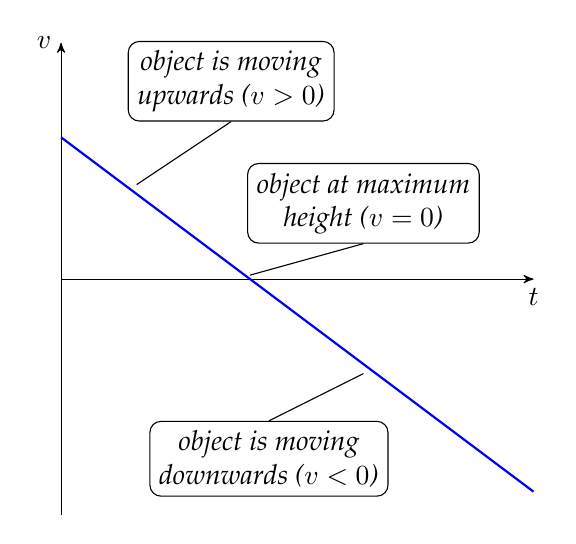
\begin{tikzpicture}[xscale=1.2]
		\draw[->] (0,-3) -- (0,3) node[left]{$v$};
		\draw[->] (0,0) -- (5,0) node[below]{$t$};
		\draw[thick,blue] (0,1.8) -- (5,-2.7);
		\draw (0.8,1.2) --++ (1,0.8) node[above,note]{object is moving\\ upwards ($v>0$)};
		\draw (2,0.05) --++ (1.2,0.4) node[above,note]{object at maximum\\height ($v=0$)};
		\draw (3.2,-1.2) --++ (-1,-0.6) node[below,note]{object is moving\\downwards ($v<0$)};
		\end{tikzpicture}
	\end{minipage}\hfil
	\centering
	\begin{minipage}{0.45\textwidth}
		\centering
		\begin{tikzpicture}[xscale=1.2]
		\draw[->] (0,-3) -- (0,3) node[left]{$s$};
		\draw[->] (0,0) -- (5,0) node[below]{$t$};
		\draw[thick,blue,domain=0:5,smooth] plot (\x,{-0.5*\x*(\x-4)});
		\draw (2.05,2.05) --++ (1,0.4) node[right,note]{maximum height\\ $h_\tmax$};
		\draw (3.3,1.1) --++ (-0.15,-0.4) node[left,note]{object above point\\of release ($h>0$)};
		\draw (4.4,-1) --++ (-0.8,-0.6) node[left,note]{object below point\\of release ($h<0$)};
		\end{tikzpicture}
	\end{minipage}

\caption*{$v$-$t$ graph and $s$-$t$ graph for upward projectile motion}
\end{figure}

\cmt sign of $v$ now gives direction of motion

$v>0$ means object is moving upwards, $v<0$ means it has reversed direction and starts falling

in particular, object attains greatest height when $v=0$

\cmt sign of $s$ gives whether object is at a higher or lower position with respect to point of release

$s>0$ means the object is above the position from which it is projected

$s<0$ means it is now below the point of release

\example{A ball is projected vertically upwards at $12 \mps$. Air resistance is negligible. (a) Find the time taken for the ball to reach the highest position. (b) Find the greatest height.}
	
\sol maximum height is reached when $v=0$, so

{
	\centering
	
	$v = u-gt = 0 \RA t= \frac{u}{g} = \frac{12}{9.81} \approx 1.22 \text{ s}$
	
	$H_\tmax = ut-\frac{1}{2}gt^2 = 12\times1.22 - \frac{1}{2}\times9.81\times1.22^2 \approx 7.34 \text{ m}$
	
}

it is also possible to use $v^2 - u^2 = 2as$ to find $H_\tmax$, this is:
\begin{equation*}
0^2 - u^2 = 2(-g)H_\tmax \RA H_\tmax = \frac{u^2}{2g} = \frac{12^2}{2\times9.81} \approx 7.34 \text{ m} \teoe
\end{equation*}

\example{A stone is thrown vertically upwards with an initial velocity of $14.0\mps$	from the edge of a cliff that is 35 m from the sea below.  (a) Find the speed at which it hits the sea. (b) Find the time taken for the stone to hit the sea.}

\sol take positive direction to point upwards, we use $v^2 - u^2 = 2as$ to find

{
	\centering
	
	$v^2 = 14.0^2 + 2\times(-9.81)\times(-35) \approx 883 \text{ m}^2 \text{ s}^{-2} \RA v\approx -29.7\mps$\footnote{Note that we have substituted  $a=-g$ since acceleration of free fall always points downwards, and $s=-35\text{ m}$ since sea is below point of release. Also final velocity when hitting water is downwards, which should take a negative sign, so we discarded the positive solution for $v$.}
	
}

to find time, we can use $v = u-gt$, hence: $ t = \frac{v-u}{-g} = \frac{-29.7-14.0}{-9.81} \approx 4.46 \text{ s} $

one can also attempt $s = ut - \frac{1}{2}gt^2$, this leads to the equation: $-35 = 14.0t - \frac{1}{2}\times9.81t^2$

this quadratic equation in $t$ gives two roots: $t_1 \approx 4.46 \text{ s}$, and $t_2 \approx -1.60 \text{ s}$

negative root should be discarded since it means stones hits the sea below it is thrown

so time taken for stone to hit the sea is $t \approx 4.46\text{ s}$ \eoe





\subsection{motion in two dimensions -- projectile motion}\label{ch:projectile}

a \keypoint{projectile} is an object whose motion is only affected by gravity\index{projectile}

for projectile motion, we assume no air resistance and no other forces

gravity causes a constant acceleration of free fall that acts vertically downwards

\cmt curved path of a projectile is the combination of its \emph{horizontal} and \emph{vertical} motion

\titem horizontally: no acceleration, so horizontal component of velocity $v_x = \text{constant}$

\titem vertically: constant acceleration, vertical component of velocity $v_y$ varies over time

as a consequence, a projectile would follows a \emph{parabolic} path as it travels\footnote{You may be able to prove this statement in Question \ref{Q-projectile-eqn}.}


\vspace*{\baselineskip}

let's consider a projectile launched at initial velocity $u$ at angle $\theta$ to the horizontal

\begin{figure}[htp]
	\centering
	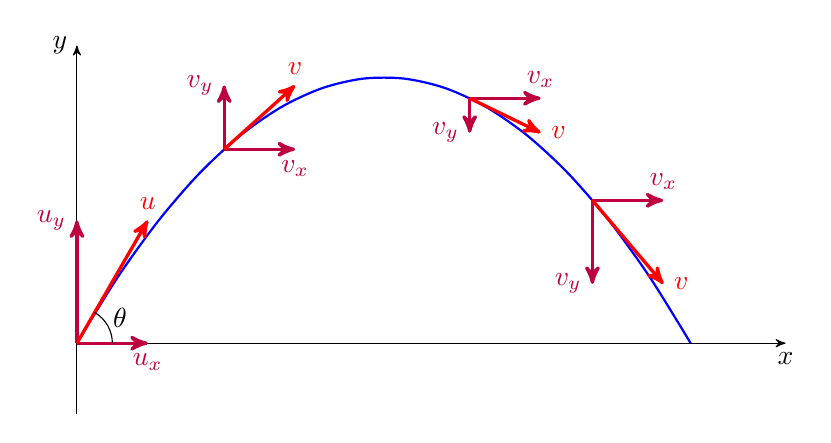
\begin{tikzpicture}[scale=.9]
	\draw[->] (0,-1) -- (0,4.2) node[left]{$y$};
	\draw[->] (0,0) -- (10,0) node[below]{$x$};
	\draw [thick,blue,domain=0:5*sqrt(3),samples=16,smooth,variable=\x] plot (\x,{sqrt(3)*\x-\x*\x/5});
	\draw[->,purple,very thick] (0, 0) -- ++(1,0) node[below]{$u_x$};
	\draw[->,purple,very thick] (0,0) -- ++(0,1.732) node[left]{$u_y$};
	\draw[->,red,very thick] (0,0) -- ++(1,1.732) node[above]{$u$};
	\foreach \idx in {1.2}
	{
		\draw[->,purple,very thick] (1.732*\idx, 3*\idx-.6*\idx*\idx) -- ++(1,0) node[below]{$v_x$};
		\draw[->,purple,very thick] (1.732*\idx, 3*\idx-.6*\idx*\idx) -- ++(0,1.732-0.693*\idx) node[left]{$v_y$};
		\draw[->,red,very thick] (1.732*\idx, 3*\idx-.6*\idx*\idx) -- ++(1,1.732-0.693*\idx) node[above]{$v$};
	}
	\foreach \idx in {3.2,4.2}
	{
		\draw[->,purple,very thick] (1.732*\idx, 3*\idx-.6*\idx*\idx) -- ++(1,0) node[above]{$v_x$};
		\draw[->,purple,very thick] (1.732*\idx, 3*\idx-.6*\idx*\idx) -- ++(0,1.732-0.693*\idx) node[left]{$v_y$};
		\draw[->,red,very thick] (1.732*\idx, 3*\idx-.6*\idx*\idx) -- ++(1,1.732-0.693*\idx) node[right]{$v$};
	}
	\draw (0.5,0) arc(0:60:0.5);
	\node at (30:0.7) {$\theta$};
	\end{tikzpicture}
	\caption*{components of the velocity of a projectile at different points along its path}
\end{figure}

\cmt horizontally, projectile maintains a constant velocity, so
\begin{equation*}
v_x = u_x \qquad x=u_x t
\end{equation*}

where $u_x = u\cos\theta$ is horizontal component of initial velocity

\cmt vertically, if upward direction is taken to be positive, then acceleration $a=-g$, so
\begin{equation*}
v_y = u_y + at = u_y - gt  \qquad y = u_y t + \frac{1}{2}at^2 = u_y t - \frac{1}{2}gt^2
\end{equation*}

where $u_y = u\sin\theta$ is vertical component of initial velocity

\cmt components can be combined to give resultant velocity or resultant displacement:
\begin{equation*}
 v = \sqrt{v_x^2 + v_y^2} \qquad s = \sqrt{x^2 + y^2}
\end{equation*}


\subsubsection*{maximum height reached by an projectile}

when a projectile reaches the highest position, its instantaneous vertical velocity becomes zero

we can then find the time it takes to attain this maximum height.
\begin{equation*}
	v_y = u\sin\theta - gt = 0 \RA t = \frac{u\sin\theta}{g}
\end{equation*}
	
to find $H_\tmax$, one can use either equation \eqref{eqn:const_a_eq2} or \eqref{eqn:const_a_eq3} 
	\begin{equation*}
	H_\tmax = \frac{1}{2}(u_y+v_y) t = \frac{1}{2}u_y t = \frac{1}{2} \times u \sin\theta \times \frac{u\sin\theta}{g} = \frac{u^2 \sin^2\theta}{2g}
	\end{equation*}
	\begin{equation*}
	H_\tmax = u_y t - \frac{1}{2}gt^2 = u \sin\theta \times \frac{u\sin\theta}{g} - \frac{g}{2} \times \left(\frac{u\sin\theta}{g}\right)^2 = \frac{u^2 \sin^2\theta}{2g}
	\end{equation*}

\cmt for the same initial speed $u$, the greater the angle of projection, the higher the object can get

in the extremal case where $\theta = 90 ^\circ$, it simply becomes an upward projection motion

\subsubsection*{airborne time and horizontal range of an projectile}

a ball projected from the ground will first rise in height

but it will eventually fall to the ground due to the gravitational pull after a period of time $T$

when it lands, its vertical displacement is zero, so
	\begin{equation*}
	Y = u_y T - \frac{1}{2}gT^2 = u \sin \theta T - \frac{1}{2}gT^2 = 0 \RA T = \frac{2u\sin\theta}{g}
	\end{equation*}
	
the horizontal range is given by
	\begin{equation*}
	X = u_x T = u\cos\theta \times \frac{2u\sin\theta}{g} = \frac{2u^2\sin\theta\cos\theta}{g} \RA X = \frac{u^2\sin2\theta}{g}
	\end{equation*}
	
where in the last step the trigonometric identity $\sin2\alpha = 2\sin\alpha\cos\alpha$ has been used

\cmt for same initial speed $u$, projectile launcher at greater angle stays in air for longer time

greatest airborne time is obtained if object is projected straight up, i.e.,  $\theta =90^\circ$

\cmt for same initial speed, horizontal range of projectile depends on angle $\theta$ of projection

to obtain the greatest horizontal range, two things are required

\titem sufficiently large horizontal velocity $v_x$

\titem sufficiently long time $T$ staying in the air

however, a larger $v_x$ requires a smaller $\theta$, hence a shorter airborne time $T$

therefore, there is a compromise between the two

optimal angle should be neither be too large nor too small, which can be shown to be $45^\circ$




\begin{figure}[ht]
	\centering
	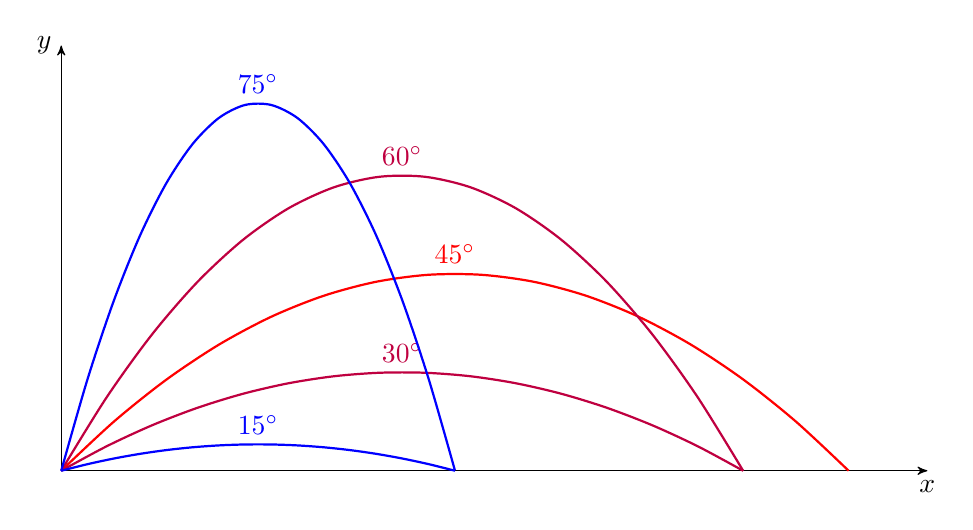
\begin{tikzpicture}[scale=1]
	\draw[<->] (0,5.4) node[left]{$y$} -- (0,0) -- (11,0) node[below]{$x$};
	\draw [thick,red,domain=0:10,samples=16,smooth,variable=\x,graphlabel={[above]{$45^\circ$}}] plot (\x,{\x-0.1*\x*\x});
	\draw [thick,purple,domain=0:5*sqrt(3),samples=16,smooth,variable=\x,graphlabel={[above]{$60^\circ$}}] plot (\x,{sqrt(3)*\x-\x*\x/5});
	\draw [thick,purple,domain=0:5*sqrt(3),samples=16,smooth,variable=\x,graphlabel={[above]{$30^\circ$}}] plot (\x,{\x/sqrt(3)-\x*\x/15});
	\draw [thick,blue,domain=0:5,samples=16,smooth,variable=\x,graphlabel={[above]{$75^\circ$}}] plot (\x,{3.732*\x-\x*\x/1.34});
	\draw [thick,blue,domain=0:5,samples=16,smooth,variable=\x,graphlabel={[above]{$15^\circ$}}] plot (\x,{0.268*\x-\x*\x/18.66});
	\end{tikzpicture}
	\caption*{trajectories of projectiles launched at the same speed but different angles}\label{fig:projectile_range}
\end{figure}


\example{A ball is thrown from a point $O$ at $15 \mps$ at an angle of $40^\circ$ to the horizontal. The ball reaches its highest position at point $P$. Ignore the effects of air resistance. (a) How long does it take to reach $P$? (b) What is the magnitude of the displacement $OP$?}
		
\sol at highest point: $v_y = u_y - gt = 0 \RA t = \frac{u\sin\theta}{g} = \frac{15\times\sin40^\circ}{9.81} \approx 0.983 \text{ s}$

vertical displacement: $y = u_y t - \frac{1}{2}gt^2 = 15\sin40^\circ \times 0.983 - \frac{1}{2}\times 9.81 \times 0.983^2 \approx 4.74 \text{ m}$

horizontal displacement: $x = u_x t = 15\cos40^\circ \times 0.983 \approx 11.3 \text{ m}$

resultant displacement: $|OP| = \sqrt{x^2 +y^2} = \sqrt{11.3^2 + 4.74^2} \approx 12.2 \text{ m}$ \eoe

\newpage

\example{A small object is horizontally projected at 7.20 ms$^{-1}$ from a surface at a height of $h=1.2 \text{ m}$ above the ground. Assume there is no air resistance. (a) What is the time taken for the object to hit the ground? (b) What is the horizontal range? (c) Find the velocity at which the object hits the ground.}

\sol vertically, take downward as positive: $h = \cancelto{0}{u_y t} + \frac{1}{2}gt^2 \ra t = \sqrt{\frac{2h}{g}} = \sqrt{\frac{2\times1.2}{9.81}} \approx 0.495 \text{ s} $

horizontal range: $x = u_x t = 7.20 \times 0.495 \approx 3.56 \text{ m}$

final vertical velocity: $v_y = \cancelto{0}{u_y} + gt = 9.81 \times 0.495 \approx 4.85 \mps$

magnitude of resultant velocity: $v = \sqrt{v_x^2 + v_y^2} = \sqrt{7.20^2 + 4.85^2} \approx 8.68 \mps$

angle to which resultant velocity makes with horizontal: $\phi = \tan^{-1}\frac{v_y}{v_x} = \tan^{-1}\frac{4.85}{7.20} \approx 34^\circ$ \eoe


\ifthenelse{\includequestions=1}{

\subsection{end-of-chapter questions}

\subsubsection*{kinematic quantities}

\question{What is the distance covered for a car that travels half a lap along a circular path of radius of 200 m. What about the displacement?}

\question{A ball is released from a height of 2.0 m above the ground. It bounces vertically for quite a number of times before coming to rest. (a) State the change of displacement for the ball. (b) Explain how the distance travelled is different from the change in displacement.}


\question{For an athlete running around a track for many laps, suggest how his average velocity could be zero?}

\question{A car travels 2400 m east in 3.0 minutes, then takes a left turn, and then travels 700 m north in 1.5 minutes. What is the average speed and the average velocity for this journey?}

\question{Is it possible for an object moving at a steady speed to have acceleration?}


\subsubsection*{motion graphs}

\question{For the $v$-$t$ graph given in Example \ref{ex-vgraph}, sketch the $a$-$t$ graph for this motion.}

\question{If the tangent of a displacement-time graph at one particular instant is sloping downwards, what does that imply about the velocity at that instant?}

\question{A vehicle initially travels at a steady speed of $15 \mps$. It accelerates uniformly for 10 s to reach a higher speed of $20 \mps$. It maintains at this speed for 20 s, and then decelerates uniformly to a stop in the last 10 s. (a) Sketch the velocity-time graph for this motion. (b) Sketch the acceleration-time graph. (c) Find the distance travelled during the 40 s.}


\subsubsection*{linear motion with constant velocity}

\question{Sonar is a technique that uses sound waves to detect objects. It can be used to measure the depth of the seabed. Given that speed of sound in water is $1500 \mps$, and reflected waves sent from a submarine are detected 0.50s after they are transmitted. How deep is the water below the submarine?}

\question{Given that the speed of sound in air is $340 \mps$ and the speed of light in air is $3.0\times10^8 \mps$. If a person hears the sound of a thunder 5.0 seconds after seeing a lightning flash, how far away from this person is did the lightning strike?}



\subsubsection*{linear motion with constant acceleration}


\question{A train initially travels at a speed of $40\mps$. It starts to decelerate at 0.50\mpss. (a) What is the distance travelled in 50 s? (b) When it comes to a stop, how far out has it travelled?}

\question{A vehicle moving at $14\mps$ accelerate uniformly to $26\mps$ in 6.0 s. (a) What is the average velocity during this time? (b) What is the acceleration during this time (c) What is the distance travelled by the vehicle? (d) The vehicle then braked with constant deceleration to stop in another 8.0 s. What is the distance travelled during the time when brakes are applied?}


\subsubsection*{free fall}


\question{Two balls are dropped from rest from the same height. The second ball is released 0.80 s after the first one. What is their separation 1.5 s after the second ball is dropped?}

\question{A golf ball is dropped from the top of a tower of height 30 m. The ball falls from rest and air resistance is negligible. What time is taken for the ball to fall (a) the first 10 m from rest, (b) the last 10 m to the ground?}

\question{The acceleration of free fall on Pluto is about one-fifteenth of that on Earth. If it takes a time of $T$ for a rock to fall from rest a distance of $S$, what is the time taken, in terms of $T$, for a rock to fall from rest through the same distance $S$ on Pluto?}

\question{In an experiment is carried out to determine the acceleration of free fall $g$ using a falling body. The body is released from rest from a height of $h$, the time taken $t$ for it to hit the floor is measured. (a) Find the expression that can be used to calculate the value of $g$? (b) Suggest what could lead to an overestimation for the value of $g$.}


\subsubsection*{upward projection}

\question{A ball is tossed upwards with a speed of $9.0 \mps$. (a) How long does it take to return to the same point if air resistance is negligible? (b) How does the return velocity compare with its initial velocity?}

\question{Someone wants to toss a ball onto a platform that is at a height of 20 m above him. What is the minimum initial velocity needed to launch the ball?}

\question{Someone standing at the top of a high building throws a ball straight up and another ball straight down with the same initial speed. Assume that air drag is negligible, which ball will have a greater speed when it hits the ground?}

\question{In basketball games, hang time refers to the length of time a player stays in the air after jumping from the floor. (a) It is reported that Michael Jordan is able to stay in the air for $T=1.0\text{ s}$ to do his slam-dunk tricks, estimate how high he can jump. (b) The acceleration of fee fall on the Moon is about one-sixth of that on Earth. What is the hang time of Michael Jordan if he takes off from the surface of the Moon?}


\begin{wrapfigure}{r}{0.44\textwidth}
	\centering
	\vspace*{-10pt}
	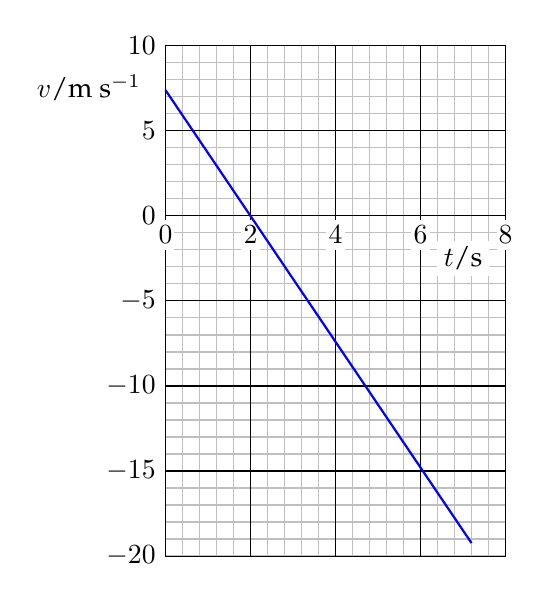
\begin{tikzpicture}[scale=1.08]
	\draw[thin, gray!50,step=0.2] (0,-4) grid (4,2);
	\draw[step=1] (0,-4) grid (4,2);
	\foreach \y in {10,5,...,-20} \node[left] at (0,\y/5){$\y$};
	\foreach \x in {0,2,...,8} 
	{
		\draw[white,fill] (\x/2-0.1,-0.4) rectangle (\x/2+0.1,-0.05);
		\node[below] at (\x/2,0) {$\x$};
	}
	\draw[thick,blue,domain=0:3.6] plot (\x, 1.48-1.48*\x); 
	\node at (-0.9,1.5) {$v$/m s$^{-1}$};
	\draw[white,fill] (3.2,-0.7) rectangle (3.8,-0.3);
	\node at (3.5,-0.5) {$t$/s};
	\end{tikzpicture}
	\vspace*{-15pt}
\end{wrapfigure}

\question{Mark Watney\footnote{A fictional character in the science fiction movie \emph{The Martian} (2015) based on the novel of the same name written by \emph{Andy Weir}.} stands at the edge of a cliff on the Mars and throws a rock vertically upwards with a speed of $7.4 \mps$. The graph shows the variation with the time $t$ of the rock's velocity $v$. (a) What is the acceleration of free fall on the Mars? (b) When does the rock reach the maximum height? (c) What is the height above the base of the cliff the moment when the rock is thrown? (d) What is the maximum height above the base of the cliff to which the rock rises? (e) What is the total distance travelled by the rock before it strikes the ground?}

\subsubsection*{projectile motion}

\question{A ball rolls off a table and lands at a position of a horizontal distance of 1.2 m from the table. The table is 0.95 m high. Find the speed at which the ball leaves the table.}

\question{A ball is kicked from the ground towards a vertical barrier. The barrier is at a horizontal distance of 18 m from the initial position of the ball. The ball strikes the barrier after 1.5 s at a height of 2.5 m above the ground. (a) Find the magnitude and the direction of the initial velocity. (b) Find the magnitude and the direction of the velocity at which the ball hits the barrier.}

\question{When a particle is launched from the origin at an angle $\theta$ with the horizontal at a speed of $u$, show that its trajectory is a parabola given by the equation: $y = x \tan\theta - \frac{gx^2}{2u^2\cos^2\theta}$.}\label{Q-projectile-eqn}

\question{Two golf players each hit a ball at the same speed. One at $30^\circ$ with the horizontal, the other at $60^\circ$. Which ball hits the ground first? Which ball goes farther?}

\question{(a) State the difference between the displacement of a projectile and the distance it travels. (b) Suggest in what situation a projectile's displacement could have the same magnitude as the distance.}

\question{An archer always aims slight higher than the distant target that she wants to hit. Why isn't the bow lined up such that it points exactly at the target?}


}{}
\section{Force \& Motion}

\subsection{force \& motion: an introduction}

in physics, a force appears when two bodies interact with one another

\cmt you will encounter various types of forces in this course, some of which are

\begin{compactitem}
	\item[--] \emph{weight}: the gravitational attraction acting on any object exerted by the earth
	
	\item[--] \emph{tension}: a force in a string, a rope, a chain, etc. when it is being pulled
	
	\item[--] \emph{normal contact}: when a body's surface is compressed, there reacts a normal contact force\footnote{Examples of normal contact force are support force that stops a desk from sinking into the ground, and the impact on a football when you kick it, etc.}
	
	\item[--] \emph{friction}: a force that resists relative motion when two surfaces tend to slide over one another
	
	\item[--] \emph{resistance}: also called drag force, this is experienced when a body travels through a medium

	
	\item[--] \emph{upthrust}: an upward force acting on an object immersed in a fluid
	
	\item[--] \emph{electric force}: an attractive or repulsive interaction between electrically charged objects
	
%	\item[--] \emph{magnetic force}: an attractive or repulsive interaction between magnets or electric currents
\end{compactitem}

detailed features of these forces follow later in the notes.

\cmt a force can produce various effects to the object, the effect could be

\begin{compactitem}
	\item[--] an increase/decrease in speed
	
	\item[--] a change in the direction of motion
	
	\item[--] causing the object to rotate
	
	\item[--] a change in shape of the object
\end{compactitem}

in this and the next few chapters, we will be looking into each of these aspects

\cmt when more than one force act on a body, it is useful to find their \emph{resultant}, or the \emph{net force}

\begin{ilight}
	\keypoint{resultant force}, or \keypoint{net force}, is a single force that has the same effect as all forces acting on an object combined
\end{ilight}

\emph{vector sum} of all of the individual forces gives the resultant force

\cmt in this chapter, we will study the dynamics of \emph{point masses}

\keypoint{point mass} is an idealization that the object has a mass but does not take up any space

position of an object treated as a point mass is specified with a geometric point in space

this is a simplification when size, shape, rotation, or structure of object are not important




\subsection{Newton's laws of motion}\index{Newton's laws of motion}

Newton's laws of motion\footnote{These three laws were first addressed by \emph{Isaac Newton} in his famous work \emph{Mathematical Principles of Natural Philosophy}, or simply the \emph{Principia}. The three-volume work was first published in 1687, and was soon recognised as one of the most important works in the history of science. Apart the from the three laws that laid the foundations for classical mechanics, the \emph{Principia} also stated \emph{the law of gravitation}, and accounted for planetary orbits and tides and other phenomena.} are three laws that form the basis of classical mechanics

they describe the relationships between motion of an object and forces acting on it


\subsubsection{first law}

\begin{ilight}
	\keypoint{Newton's first law} states that an object continues in its state of rest or uniform motion at constant velocity if there is no resultant force acting
\end{ilight}


\cmt any object `dislikes' any change to its state of motion, uniform motion tends to persist forever

this tendency to resist changes in motion is called the \keypoint{inertia}

Newton's first law is also called \emph{the law of inertia}

\cmt if there is no change in state of motion, the object is said to be in \keypoint{equilibrium}\index{equilibrium}

equilibrium could be either \emph{static} (being at rest) or \emph{dynamic} (steadily moving in a straight line)

both cases require zero resultant force

\cmt Newton’s law of inertia is placed to establish frames of reference

it is in an reference frame that notions of displacement, velocity and acceleration can be defined

an \keypoint{inertial reference frame} is one in which Newton’s laws hold
\footnote{Inertial frame is not unique. An observer moving at constant velocity to an inertial observer is in a different inertial frame, since constant velocity of object added to a constant relative velocity is still a constant velocity. Two inertial observers would disagree on a body's velocity, but they would agree that the body maintains its velocity in absence of net force, i.e., they will observe the same physics phenomena. This is known as the \emph{equivalence principle}.}

%\begin{example}{Suspension of a slinky}
%	If a slinky is freely suspended, one notices that the degree to which the slinky is stretched increases uniformly with height.
%	
%	Since the slinky is in a state of rest, all net force is cancelled throughout the entire slinky, i.e., the tension at any point balances the weight of the slinky beneath it. So the higher it goes, the more weight is supported, so the top bit has to be stretched more to provide a greater tension to hold the bottom part.
%\end{example}


\subsubsection{second law}

if resultant force is non-zero, velocity of the object will change, i.e., force produces acceleration


\begin{ilight}
	\keypoint{Newton's second law} states that the acceleration is proportional to the resultant force and inversely proportional to the mass of the object
\end{ilight}

\cmt symbolically, we write $a \propto \frac{\fnet}{m}$

with consistent units of measure, this proportionality can be written as an exact equation:
\begin{equation}
a=\frac{\fnet}{m} \quad \text{or} \quad \boxed{\fnet=ma}
\end{equation}

\cmt SI unit of measurement for force $F$ is \keypoint{newton} (N)

a force of one newton acting a body of 1 kg produces an acceleration of 1 $\mpss$

\cmt note that the force in the equation $F=ma$ is the resultant force

to determine change in motion for a body, you should always ask what the resultant force is

\cmt acceleration produced is always in same direction of the net force

\cmt for same force, an object of greater mass has a smaller acceleration

hence mass is a measure of the \emph{inertia} of this object in response to a net force\index{inertia}

a definition for mass of an object from the point of view of Newton's laws can be stated as\footnote{The concept of mass can be defined in many different ways. You might be familiar with the definition for mass as the amount of matter an object possesses. I personally think this definition is a bit vague and does not tell you anything new. Thinking of mass as a measure of inertia surely brings more insights. Mass also tells the strength at which an object interacts with other bodies through the gravitational attraction. As you will see later, from the view of Albert Einstein, it is also possible to think of mass as a form of energy, which is my favourite definition for mass.}:

\begin{ilight}
	\keypoint{mass} is an intrinsic property of a body to resist any change in its state of motion
\end{ilight}

\example{A box of 6.0 kg is being pushed along a horizontal surface with a force of 30 N. The resistive force acting is 21 N. What is the acceleration of the box?}

\solc\begin{equation*}
	\fnet = F - f = ma \RA a = \frac{F-f}{m} = \frac{30-21}{6.0} = 1.5 \mpss \teoe
\end{equation*}

\example{A car of mass 800 kg is travelling at a speed of $20 \mps$. The driver then operates the brake pedal so a braking force of 2000 N gradually brings the car to stop. (a) What is the deceleration for the car? (b) What is the stopping distance?}

\sol using Newton's second law and noticing braking force acts opposite to direction of motion:

{
	\centering
	
	$\fnet = ma \RA -2000 = 800 \times a \RA a = -2.5 \mpss$
	
	$2as = v^2 - u^2 \RA s = \frac{v^2-u^2}{2a} = \frac{0^2 - 20^2}{2\times(-2.5)} = 80\text{ m}$
	
}

\feoe



	\begin{wrapfigure}{R}{0.2\textwidth}
		\vspace{-18pt}
		\begin{center}
			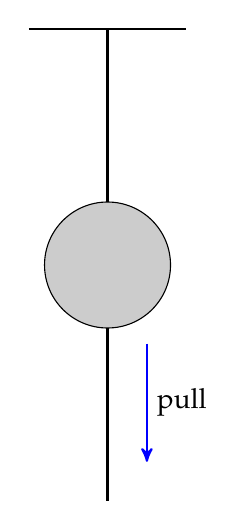
\begin{tikzpicture}[scale=1]
			\draw[thick] (-1,6) -- (1,6);
			\draw[thick] (0,6) -- (0,0);
			\draw[thick, ->, blue] (.5,2) -- (.5,0.5) node[midway, right]{\textcolor{black}{pull}};
			\draw[fill=gray!40] (0,3) circle[radius=.8];
			\end{tikzpicture}
		\end{center}
		\vspace{-20pt}
	\end{wrapfigure}
	
\example{A massive ball is suspended on a string. A second string is attached to the bottom of the ball. If one pulls the bottom string with a gradually increasing force, does the top string or the bottom string break first? What if the bottom string is jerked, which string breaks?}	
	
\sol when tension gradually increases, system is always in equilibrium

tensions in strings must have $T_\text{top} = T_\text{bottom} + mg$

top string suffers a greater force, so it breaks first
	
however, when bottom string is jerked, the ball tends to remain at rest due to its large mass, preventing sudden change to the tension in top string

so in this case bottom string is more likely to snap \eoe

%\begin{example}{Leviation of a slinky}
%	When the top end of the slinky is dropped, the information of the tension change must propagate to the bottom end before both sides begin to fall; the top of an extended slinky will drop while the bottom initially remains in its original position, compressing the spring.
%\end{example}




\subsubsection{third law}

every force is part of a pair of interactions between one body and another

when one body exerts a force on another, the second body also exerts a reaction on the first

\begin{ilight}
	\keypoint{Newton's third law}, also called the \keypoint{action-reaction principle}, states that action and reaction are always equal in magnitude, opposite in directions and of the same type
\end{ilight}

\example{Suggest the action and reaction force in the following cases: (a) A man stands on a bathroom scale. (b) A helicopter hovers in air. (c) The earth orbits around the sun.}

\sol (a) man exerts downward force on scale, scale exerts an upward reaction on man

(b) rotors of helicopter push air downwards, air exerts an upward force on helicopter

(c) sun pulls the earth through gravitational attraction, earth also attracts the sun in return \eoe


\subsubsection{force analysis \& free-body diagrams}

when doing mechanics problems, it is necessary to find all forces applied upon an object

to visualise all these forces, it is helpful to draw a \keypoint{free-body diagram} (FBD)\index{free-body diagram}

an FBD shows a simplified version of the body with arrows indicating forces applied

\newpage

it is recommended to follow the routine stated below when solving a mechanics problem

\begin{compactitem}
	\item[(1)] draw a FBD for the object in the problem
	
	\item[(2)] resolve and find the resultant force with aid of the FBD
	
	\item[(3)] apply Newton's laws to write down the equation of motion for the object
	
	\item[(4)] solve the equation(s) to find acceleration
	
	\item[(5)] use kinematic relations to deduce information about motion of the object
\end{compactitem}


% % % % % % % % % % % % % % % % % % % %

\subsection{types of forces}

\subsubsection{weight}\label{ch_weight}

all objects exert attractive forces of gravity upon each other\footnote{You will learn more about gravitational forces at A2 Level.}

\keypoint{weight} of a body is due to the gravitational pull from our planet -- the earth\index{weight}

weight $W$ of any object is proportional to its mass $m$: $\boxed{W=mg}$

$g$ is called the gravitational field strength, or the gravitational acceleration constant

\cmt at vicinity of earth's surface, gravitational field is almost uniform: $g \approx 9.81 \text{ N kg}^{-1}$

but this value for $g$ does not hold in a satellite orbit, on Mars, near a black hole, etc.

\cmt the concept of weight is different from mass in many aspects

\begin{compactitem}
	\item[--] weight is a force, so it is a vector (always acting downwards still makes a direction)
	
	mass is a scalar, it has magnitude only
	
	\item[--] weight is measured in newtons, mass is measured in kilograms
	
	\item[--] weight of object depends on its mass but also strength of gravitational field
	
	mass is an intrinsic property of object, so does not depend on force fields
	
	same object can have different weights on different planets, but its mass will be the same\footnote{Here we do not take into account the effects of \emph{relativity}. A clever student who has learned Einstein's theories might suggest the mass of the same object increases with its velocity.}
\end{compactitem}

\example{An astronaut finds that he weighs 300 N on the surface of Mars, where the gravitational field strength is known to be $3.7 \text{ N kg}^{-1}$. Find his mass and hence estimate his weight if he returns to his home on the Earth.}

\sol mass of astronaut: $m = \frac{W_M}{g_M} = \frac{300}{3.7} \approx 81.1 \text{ kg}$

weight on earth: $W_E = mg_E = 81.1 \times 9.81 \approx 795 \text{ N}$ \eoe

\subsubsection*{free fall}

all things on the earth fall because of the force of gravity

if we ignore the restraints such as air resistance and upthrust force on a falling object, say the object is under the influence of gravity only, then the object is in a state called \keypoint{free fall}



assuming the object is subject to gravity only, the resultant force is simply its weight

applying the Newton's second law, we have: $\fnet = W \RA ma = mg$

so acceleration of the freely-falling object is: $\boxed{a=g}$\footnote{In the derivation, the mass terms cancel out. Rigorously speaking, these are two different masses. One is the measure of inertia, and the other is a measure of gravitational force. It is experimentally found that the inertia mass and the gravitational mass are equal. The fact that the two masses are equal has profound reasons. We have shown here acceleration of free fall equals gravitational field strength, but Albert Einstein’s suggests that it is actually impossible to distinguish between a uniform acceleration and a uniform gravitational field. This idea lies at the heart of his \emph{general theory of relativity}. Those who are interested in this topic are recommended to start from here and do some online researches.}

\cmt this shows \keypoint{acceleration due to free fall} is simply equal to field strength $g$

so any object, regardless of its mass, has same acceleration due to free fall\footnote{In \S\ref{ch_freefall} and \S\ref{ch:projectile}, the statement that acceleration of free fall is constant in absence of air resistance was asserted without further explanation. Now you know why.}


\subsubsection{drag}

when a body moves through air, water or any fluid, it experiences resistance called drag force\index{drag}

\cmt factors that determine the value of fluid drag include

\titem relative speed of the object to the fluid ($v\up \ra f\up$)

\titem cross section of the object ($A\up \ra f\up$)

\titem shape of the object (streamlined shape has smaller drag)

\titem density of the fluid ($\rho\up \ra f\up$)

but what determines the drag force is a complicated issue\footnote{There are a few empirical formula for drag force, each of which is accurate under certain conditions.
	
	For an object moving through a fluid at low speeds (\emph{laminar flow}, no turbulence occurs), the resistance it experiences is proportional to its speed: $f=bv$, where $b$ is some constant which depends on fluid viscosity and the effective cross-sectional area of the object.
	
	If objects are moving at relative high speeds through the fluid such that \emph{turbulence} is produced behind the object, drag force is proportional to the speed squared: $ f = \frac{1}{2} \rho C_D A v^2$, where $\rho$ is the fluid's density, $A$ is the cross-sectional area, $C_D$ is a dimensionless quantity called the drag coefficient.}

\cmt drag force always acts in a direction to oppose relative motion of object through fluid




\subsubsection*{free fall through air}

\begin{wrapfigure}{r}{0.15\textwidth}
	\vspace*{-16pt}
	\centering
	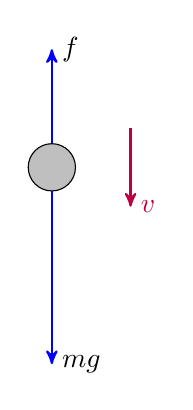
\begin{tikzpicture}
	\draw[thick,blue,->] (0,0) -- (0,-2.5) node[right,black]{$mg$};
	\draw[thick,blue,->] (0,0) -- (0,1.5) node[right,black]{$f$};
	\draw[fill=gray!50] (0,0) circle (0.3);
	\draw[thick,purple,->] (1,0.5) -- (1,-0.5) node[right]{$v$};
	\end{tikzpicture}
	\vspace*{-16pt}
\end{wrapfigure}

let's consider an object falling through air from a very high tower

forces acting are weight and air resistance (shown in the free-body diagram)

equation of motion for this falling object is:

{
	\centering
	
	$ \fnet = mg - f = ma $
	
}

as $v$ increases, air resistance $f$ increases, so net force $\fnet$ decreases

this means acceleration $a$ would decrease as object falls

i.e., speed will increase at a decreasing rate during the fall
\footnote{The velocity-time relation can be obtained for some simple models. Suppose air resistance is proportional to speed of the falling body, i.e., $f=bv$, then the equation of motion reads: $\fnet = m \frac{\dd v}{\dd t} = mg - bv$, where acceleration is written explicitly as the rate of change in velocity. With the initial conditions $v=0$ at $t=0$, we can solve this differential equation to obtain the speed of this falling object at any given time $t$:
\begin{equation*}
	\dd t = \frac{\dd v}{g - \frac{b}{m}v} \RA \int_0^t \dd t = \int_0^v \frac{\dd v}{g - \frac{b}{m}v} \RA t = -\frac{m}{b} \ln \left(g - \frac{b}{m}v \right) \Bigg|_0^v = -\frac{m}{b} \ln \left( 1 - \frac{bv}{mg}\right)
\end{equation*}
	
Rearrange the terms, we find: $v(t) = \frac{mg}{b} \left(1 - \ee^{-\frac{bt}{m}} \right) $}

%$v$-$t$ graph for this process is shown on the next page


\begin{figure}[ht]
	\centering
	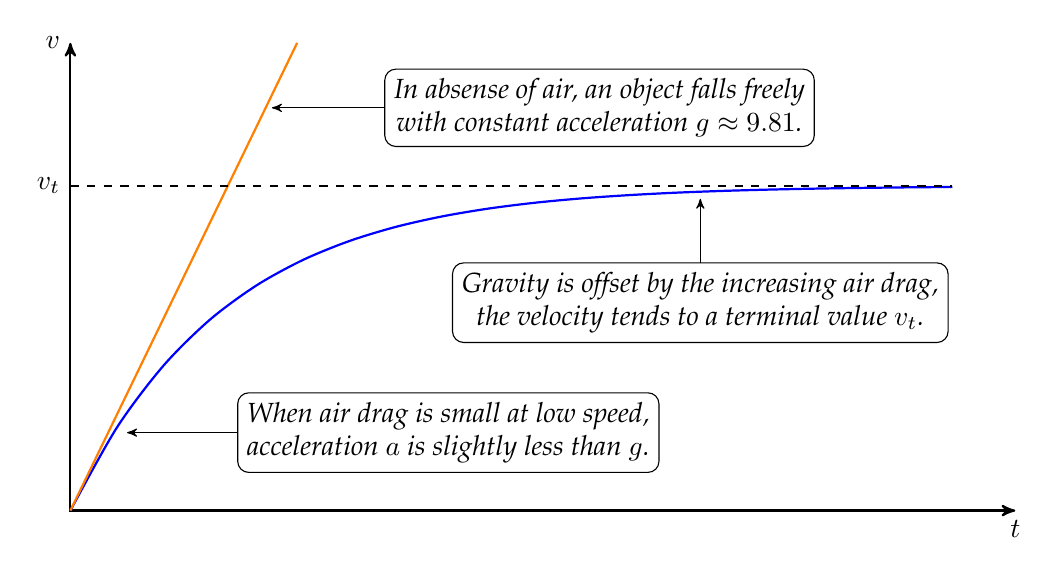
\begin{tikzpicture}[xscale = 1.6,yscale=1.65]
	\draw [thick, <->] (7.5,0) node[below]{$t$} -- (0,0) --(0,3.6) node[left]{$v$};
	\draw [thick,blue,domain=0:7,samples=20,smooth,variable=\x] plot (\x,{2.5*(1-exp(-0.8*\x))});
	\draw [thick,orange] (0,0) -- (1.8,3.6);
	\draw [thick,dashed] (0,2.5) node[left]{$v_t$} -- (7,2.5);
	\draw [->] (3,0.6) node[note]{When air drag is small at low speed,\\ acceleration $a$ is slightly less than $g$.} -- (0.45,0.6);
	\draw [->] (5,1.6) node[note]{Gravity is offset by the increasing air drag, \\ the velocity tends to a terminal value $v_t$.} -- (5,2.4);
	\draw [->] (4.2,3.1) node[note]{In absense of air, an object falls freely \\ with constant acceleration $g\approx9.81\mpss$.} -- (1.6,3.1);
	\end{tikzpicture}
	\caption*{variation of velocity for a falling object through air}
\end{figure}

\cmt after sufficient long time, acceleration gradually decreases to zero

velocity gradually increases and tends to a maximum value

at this stage, equilibrium is restored: $f=mg$, object no longer accelerates

this constant final velocity is known as the \keypoint{terminal velocity}\index{terminal velocity}

\cmt at low speeds, air resistance is negligible, so $\fnet =ma \approx mg$

acceleration of object at start of the fall is similar to $g$

but as $v$ increases, acceleration decreases so $a$ becomes less than $g$




\example{An object of 5.0 kg falls through the atmosphere from a very high altitude. After some time, it falls at a constant speed of $70 \mps$. Assume there is no significant change in gravitational field during the fall and the air resistance is proportional to speed: $f=bv$. (a) Find the value of the coefficient $k$. (b) Find the acceleration of the object when it is falling at $30\mps$.}

\sol equilibrium between weight and air drag when falling at terminal speed, so
\begin{equation*}
	mg = bv_t \RA b = \frac{mg}{v_t} = \frac{5.0\times9.81}{70} \approx 0.70 \text{ kg s}^{-1}
\end{equation*}

at any instant, equation of motion is: $\fnet = ma = mg - bv$

at $30\mps$, acceleration is: $a = \frac{mg-bv}{m} = \frac{5.0\times9.81-0.70\times30}{5.0} \approx 5.6 \mpss$ \eoe

\subsubsection*{bubble rising in a liquid}

\begin{wrapfigure}{r}{0.15\textwidth}
	\vspace*{-16pt}
	\centering
	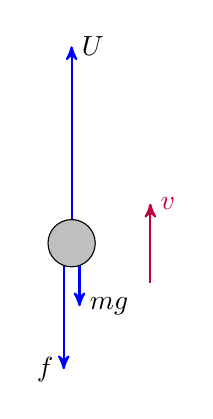
\begin{tikzpicture}
	\draw[thick,blue,->] (0.1,0) -- (0.1,-0.8) node[right,black]{$mg$};
	\draw[thick,blue,->] (-0.1,0) -- (-0.1,-1.6) node[left,black]{$f$};
	\draw[thick,blue,->] (0,0) -- (0,2.5) node[right,black]{$U$};
	\draw[fill=gray!50] (0,0) circle (0.3);
	\draw[thick,purple,->] (1,-0.5) -- (1,0.5) node[right]{$v$};
	\end{tikzpicture}
	\vspace*{-16pt}
\end{wrapfigure}

let's now consider bubbles formed at the bottom of a soda water

forces acting on bubble are weight, water resistance and upthrust

equation of motion for the rising bubble is:

{
	\centering
	
	$ \fnet = U - mg - f = ma $
	
}

as bubble moves faster, $f$ increases, then $\fnet$ decreases

so acceleration $a$ would gradually decrease to zero as bubble rises

speed of bubble increases and reaches a maximum value

at terminal speed, $a\to0$, one has: $U=f+mg$



\subsubsection{normal contact}

when two objects are in contact, the interaction between them is called the \emph{contact force}

\keypoint{normal contact force} is the component of contact force that is perpendicular to contact surface

\cmt by definition, normal contact is always at right angle to surface of contact

\cmt origin of normal contact is the \emph{electrostatic interaction} between atoms

when two objects are pressed against each other, surface atoms get close

\begin{wrapfigure}{r}{0.3\textwidth}
	\vspace*{-10pt}
	\centering
	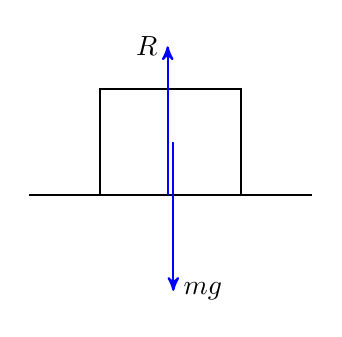
\begin{tikzpicture}[scale=0.9]
	\draw[thick] (-2,0) -- (2,0);
	\draw[thick] (-1,0) rectangle (1,1.5);
	\draw[thick,blue,->] (0.04,0.75) --++ (0,-2.1) node[right,black]{$mg$};
	\draw[thick,blue,->] (-0.04,0) --++ (0,2.1) node[left,black]{$R$};
	\end{tikzpicture}
	\vspace*{-5pt}
\end{wrapfigure}

electrostatic repulsion between electron clouds of the atoms prevent them from penetrating through one another


\example{A box of mass $m=4.0 \text{ kg}$ is resting on a horizontal ground. What is the normal contact force acting?}

\sol equilibrium between weight and normal contact, so
\begin{equation*}
	R-W=0 \RA R=mg = 4.0 \times9.81 \approx 39.2 \text{ N} \teoe
\end{equation*}

\begin{wrapfigure}{r}{0.24\textwidth}
	\vspace*{-10pt}
	\centering
	\begin{tikzpicture}[scale=0.9]
	\draw[thick] (-1,0) rectangle (1,3);
	\draw[fill, gray] (0,1.5) circle(0.25);
	\draw[ultra thick, gray] (0,1.5) -- (0,0.8) -- (-0.2,0) (0,0.8) -- (0.2,0);
	\draw[ultra thick, gray] (0,1.25) -- (-0.3,0.6) (0,1.25) -- (0.3,0.6);
	\draw[blue,fill] (0,.9) circle(0.05);
	\draw[thick,blue,->] (0,.9) --++ (0,-1.5) node[right,black]{$mg$};
	\draw[thick,blue,->] (0,.9) --++ (0,1.5) node[left,black]{$R$};
	\draw[ultra thick] (0,3) --++ (0,0.8);
	\draw[purple,thick,->] (1.5,0.8) --++ (0,1.4) node[right]{$v$};
	\end{tikzpicture}
	\vspace*{-5pt}
\end{wrapfigure}

\example{A man of $80$ kg stands in a lift. Find his apparent weight, i.e., the contact force, when the lift is (a) moving upwards at steady speed of $2.0 \mps$, (b) accelerating upwards at $2.0 \mpss$, (c) moving upwards but slowing down at a deceleration of $1.5 \mpss$.}

\sol forces acting on man are weight and normal contact

for either case, equation of motion for the man reads:

{

\centering

$\fnet = ma = R - mg$

}

so normal contact force: $R = mg + ma$

when rising at steady speed, man is in equilibrium ($a=0$), so: $R=mg = 80\times9.81 \approx 785 \text{ N}$

when accelerating upwards ($a = +2.0 \mpss$): $R = 80 \times 9.81 + 80 \times 2.0 \approx 945 \text{ N}$

when decelerating upwards ($a = -1.5 \mpss$): $R = 80 \times 9.81 + 80 \times (-1.5) \approx 665 \text{ N}$ \eoe


\example{A sleigh of mass 15 kg lies at rest on an icy ground. The surface is frictionless. A force $P$ of 75 N is applied to the sleigh. Find the normal contact force and the acceleration of the sleigh if $P$ is acting (a) horizontally, (b) at an angle $\alpha$ to the horizontal where $\tan\alpha=\frac{3}{4}$.}

\begin{wrapfigure}{r}{0.4\textwidth}
	\vspace*{-20pt}
	\centering
	\begin{minipage}[b]{0.2\textwidth}
		\centering
		\begin{tikzpicture}[scale=0.84]
		\draw[thick,fill] (0,0) circle(0.05);
		\draw[blue,thick,->] (0,0) -- (0,-3) node[right]{$mg$};
		\draw[blue,thick,->] (0,0) -- (0,3) node[right]{$R$};
		\draw[blue,thick,->] (0,0) -- (1.5,0) node[right]{$P$};
		\node at (0,-4) {(a)};
		\end{tikzpicture}
	\end{minipage}\hfil
	\begin{minipage}[b]{0.2\textwidth}
		\centering
		\begin{tikzpicture}[scale=0.84]
		\draw[thick,fill] (0,0) circle(0.05);
		\draw[blue,thick,->] (0,0) -- (0,-3) node[right]{$mg$};
		\draw[blue,thick,->] (0,0) -- (0,2.1) node[right]{$R$};
		\draw[blue,thick,->] (0,0) -- (1.2,0.9) node[right]{$P$};
		\draw[dashed] (0,0) -- (1,0);
		\draw(0.5,0) arc(0:36.89:0.5);
		\node at (19:0.8) {$\alpha$};
		\node at (0,-4) {(b)};
		\end{tikzpicture}
	\end{minipage}
\end{wrapfigure}

\sol free-body diagrams for both cases are shown

for both cases, no net force acts in vertical direction

net force in horizontal direction provides acceleration

when $P$ acts horizontally:

{
	\centering
	
	$ R = mg = 15\times 9.81 \approx 147 \text{ N}$
	
	$ P = ma \RA a = \frac{P}{m} = \frac{75}{15} = 5.0 \mpss $
		
}

when $P$ acts at angle $\alpha$:

{
	\centering
	
	$R + P\sin\alpha = mg \RA R = 15\times9.81-75\times\frac{4}{5} \approx 87 \text{ N}$
	
	\eqyskip $ P\cos\alpha = ma \RA a = \frac{P\cos\alpha}{m} = \frac{75\times\frac{3}{5}}{15} = 3.0 \mpss $
	
	\feoe
	
}



\subsubsection{friction}

friction is the component of contact force that is parallel to contact surfaces

when there is potential or actual sliding between surfaces, frictional force come into action\index{friction}

\titem for surfaces \emph{tend} to move relative to each other, \keypoint{static friction} acts to oppose this tendency

\titem if surfaces are already sliding over one another, then \keypoint{kinetic friction} opposes this motion

\cmt static friction $f_S$ is self-adjusting

an object placed on a rough surface can stay at rest when acted by a small external force $F$

it can do so because $f_S$ equalises external force to maintain equilibrium

if no external force acts, then $f_S=0$

\cmt there exists a maximum limiting friction $f_\text{lim}$

when external force $F < f_\text{lim}$, there is sufficient $f_S$ to prevent object from sliding

when $F = f_\text{lim}$, object is on the verge of sliding

when $F>f_\text{lim}$, object start to move and static friction becomes kinetic friction $f_K$

\cmt factors that determine frictional forces are

\titem nature of contacting surfaces (for both $f_S$ and $f_K$)

\titem normal reaction $R$ (for $f_K$)

these dependences are usually expressed by a mathematical equation $\boxed{f_K \approx f_\text{lim} = \mu R}$

$\mu$ is the \emph{coefficient of friction} whose value depends on the nature of the two surfaces\footnote{The idea of limiting friction is not required in the AS Physics syllabus, but it is required in \emph{Mechanics 1} of the A-Level Mathematics course.}

\cmt friction, on microscopic level, is an \emph{electromagnetic force} in nature

when two surfaces are in contact, irregularities on the surface touch each other

surface atoms come very close and bonds are formed through electrostatic force

in some sense, surface atoms get \emph{cold welded} to each other

when surfaces try to move relative to each other, this electrostatic weld is origin of friction

\subsection{inclined slope}\index{inclined slopes}

inclined slope is probably the entry ticket into the business of mechanics

this notorious problem is found in any physics textbook and any exam paper on mechanics

\begin{wrapfigure}{r}{0.48\textwidth}
%	\vspace*{-12pt}
	\centering
	\begin{tikzpicture}[scale=1]
	\draw[thick] (0,0) -- (30:5) -- ++(0,-2.5) -- cycle;
	\draw[thick] (0.8,0) arc(0:30:0.8);
	\node at (15:1) {$\theta$};
	\draw[thick] (30:2.5) -- ++(120:1) -- ++(30:1) -- ++(-60:1);
	\draw[thick] (-1,0) -- (5,0);
	\draw[thick,blue,->] (2.348,1.933) --++ (0,-1.6) node[right,black]{$W$};
	\draw[thick,blue,->] (30:3) ++ (120:0.5) --++ (120:1.4) node[left]{$R$};
	\draw[thick,blue,->] (30:3) ++ (120:0.5) --++ (30:1.8) node[above]{$F$};
	\draw[thick,blue,->] (30:3) ++ (120:0.5) --++ (210:0.8) node[left]{$f$};
	\draw[purple,thick,->] (2.7,3) --++ (30:0.8) node[midway,above]{$v$};
	%	\draw[thick,blue,->] (2.348,1.933) --++ (210:0.8) node[left]{$W_\parallelslant$};
	%	\draw[thick,blue,->] (2.348,1.933) --++ (-60:1.38564) node[right]{$W_\perp$};;
	%	\draw[dashed] (2.348,1.933) ++ (210:0.8) --++ (-60:1.38564) --++ (30:0.8) ;
	\end{tikzpicture}
	\vspace*{-16pt}
\end{wrapfigure}

the problem is about a mass $m$ placed on a plane inclined at angle $\theta$ to the horizontal

the mass could sit at rest on, slide down, or get pulled/pushed up the plane

motion of the mass could be affected by weight, friction, normal contact, or other forces

\cmt forces can be resolved in directions parallel and perpendicular to the slope

resolving along the slope leads to the equation of motion from which acceleration is found

\cmt it is almost inevitable to break weight into two components\footnote{We have already done that in Example \ref{ex:comp-of-W}.}

\titem component of weight parallel down the slope is: $W_\parallelslant = mg\sin\theta$

\titem component of weight perpendicular to slope is: $W_\perp = mg\cos\theta$

\begin{wrapfigure}{r}{0.4\textwidth}
	\centering
	\begin{tikzpicture}[scale=1.35]
	\draw[thick] (0,0) -- (20:3.5) -- ++(0,-1.1971) -- cycle;
	\draw[thick] (1,0) arc(0:20:1);
	\node at (10:1.2) {$\theta$};
	\draw[thick] (20:1.7) -- ++(110:0.6) -- ++(20:0.6) -- ++(-70:0.6);
	\draw[thick,blue,->] (20:2) ++ (110:0.3) --++ (0,-1.5) node[right,black]{$W$};
	\draw[thick,blue,->] (20:2) ++ (110:0.3) --++ (110:1.4) node[left]{$R$};
	\draw[thick,blue,->] (20:2) ++ (110:0.3) --++ (20:0.6) node[above]{$f$};
	\end{tikzpicture}
	\vspace*{-16pt}
\end{wrapfigure}

\example{A block of mass $m$ stays at rest on an inclined plane. The plane makes an angle $\theta$ with the horizontal. Find the normal contact force $R$ and the frictional force $f$ acting on the block.}

\sol block in equilibrium, so $\fnet=0$ in any direction

parallel to slope: $f = W_\parallelslant \RA f=mg\sin\theta$

normal to slope: $R = W_\perp \RA R =mg\cos\theta$ \eoe


\begin{wrapfigure}{r}{0.4\textwidth}
	\centering
	\vspace*{-16pt}
	\begin{tikzpicture}[scale=1.1]
	\draw[thick] (0,0) -- (20:5) -- ++(0,-1.71) -- cycle;
	\draw[thick] (1,0) arc(0:20:1);
	\node at (10:1.2) {$\theta$};
	\draw[thick] (20:3) -- ++(110:1) -- ++(20:1) -- ++(-70:1);
	\draw[thick,blue,->] (20:3.5) ++ (110:0.5) --++ (0,-1.5) node[right,black]{$W$};
	\draw[thick,blue,->] (20:3.5) ++ (110:0.5) --++ (110:1.4) node[left]{$R$};
	\draw[purple,thick,->] (2,2.4) --++ (200:0.8) node[midway,above]{$v$};
	\end{tikzpicture}
	\vspace*{-16pt}
\end{wrapfigure}

\example{A block of mass $m$ slides down a \emph{smooth} slope. The angle of the slope to the horizontal is $\theta$. Find the acceleration of the block.}

\sol only force acting along the slope is component of weight down the slope, so:

{
	\centering
	
	$ \fnet = ma = mg\sin\theta \RA a = g\sin\theta $
	
}

as $\theta\to0$, $a\to0$, this shows if plane becomes horizontal, the block simply stays put

as $\theta\to90^\circ$, slope becomes vertical, block would undergo free fall, so naturally $a\to g$ \eoe 


\begin{wrapfigure}{r}{0.4\textwidth}
	\vspace*{25pt}
	\centering
	\begin{tikzpicture}[scale=1.1]
	\draw[thick] (0,0) -- (20:5) -- ++(0,-1.71) -- cycle;
	\draw[thick] (1,0) arc(0:20:1);
	\node at (10:1.2) {$\theta$};
	\draw[thick] (20:3) -- ++(110:1) -- ++(20:1) -- ++(-70:1);
	\draw[thick,blue,->] (20:3.5) ++ (110:0.5) --++ (0,-1.5) node[right,black]{$W$};
	\draw[thick,blue,->] (20:3.5) ++ (110:0.5) --++ (110:1.4) node[left]{$R$};
%	\draw[thick,blue,->] (20:3.5) ++ (110:0.5) --++ (20:1.8) node[above]{$F$};
	\draw[thick,blue,->] (20:3.5) ++ (110:0.5) --++ (20:0.375) node[below]{$f$};
	\draw[purple,thick,->] (2,2.4) --++ (200:0.8) node[midway,above]{$v$};
	%	\draw[thick,blue,->] (20:3.5) ++ (110:0.5) --++ (200:0.8) node[left]{$W_\parallelslant$};
	%	\draw[thick,blue,->] (20:3.5) ++ (110:0.5) --++ (-70:1.38564) node[right]{$W_\perp$};;
	%	\draw[dashed] (2.348,1.933) ++ (210:0.8) --++ (-60:1.38564) --++ (30:0.8) ;
	\end{tikzpicture}
%	\vspace*{-16pt}
\end{wrapfigure}

\newpage

\example{A block of mass 2.0 kg slides down a rough slope from rest. The slope is inclined at angle $\theta=20^\circ$ to the horizontal, and the block experiences a constant friction of 5.0 N. (a) What is the block's acceleration? (b) What is the distance travelled in 2.5 seconds?}

\sol resolving along slope:

{
	\centering
	
	$\fnet = mg\sin\theta - f = ma$
	
	\eqyskip $a = \frac{2.0 \times 9.81\times\sin20^\circ - 5.0}{2.0} \approx 0.855 \mpss $
	
}




distance travelled: $s = \cancelto{0}{ut} + \frac{1}{2}at^2 = \frac{1}{2}\times0.855\times2.5^2 \approx 2.67 \text{ m}$ \eoe


\begin{wrapfigure}{r}{0.4\textwidth}
%	\vspace*{16pt}
	\centering
	\begin{tikzpicture}[scale=1.1]
	\draw[thick] (0,0) -- (18:5) -- ++(0,-1.545) -- cycle;
	\draw[thick] (1,0) arc(0:20:1);
	\node at (10:1.2) {$\theta$};
	\draw[thick] (18:1.5) -- ++(108:1) -- ++(18:1) -- ++(-72:1);
	\draw[thick,blue,->] (18:2) ++ (108:0.5) --++ (0,-1.4) node[right,black]{$W$};
	\draw[thick,blue,->] (18:2) ++ (108:0.5) --++ (108:1.3) node[left]{$R$};
	%	\draw[thick,blue,->] (20:3.5) ++ (110:0.5) --++ (20:1.8) node[above]{$F$};
	\draw[thick,blue,->] (18:2) ++ (108:0.5) --++ (198:0.4) node[above]{$f$};
	\draw[purple,thick,<-] (2.8,2.4) --++ (198:0.8) node[midway,above]{$v$};
	%	\draw[thick,blue,->] (20:3.5) ++ (110:0.5) --++ (200:0.8) node[left]{$W_\parallelslant$};
	%	\draw[thick,blue,->] (20:3.5) ++ (110:0.5) --++ (-70:1.38564) node[right]{$W_\perp$};;
	%	\draw[dashed] (2.348,1.933) ++ (210:0.8) --++ (-60:1.38564) --++ (30:0.8) ;
	\end{tikzpicture}
	%	\vspace*{-16pt}
\end{wrapfigure}


\example{A block of mass 3.0 kg is travelling up an inclined slope at an initial speed of $2.8 \mps$. The slope makes an angle of $18^\circ$ with the horizontal. A constant friction of 7.5 N acts on the block. (a) What is the block's deceleration? (b) How far does the block travel along the slope before its speed decreases to zero? (c) Suggest whether the block could stay on the slope.}

\sol resolving along slope (take direction of initial velocity as positive direction): 

{
	\centering
	
	$\fnet = -mg\sin\theta - f = ma \RA a = \frac{-mg\sin\theta-f}{m} = \frac{-3.0\times9.81\times\sin18^\circ-7.5}{3.0} \approx - 5.53 \mpss$
	
	\eqyskip $v^2 - u^2 = 2as \RA s = \frac{v^2 - u^2}{2a} = \frac{0^2 - 2.8^2}{2\times(-5.5.3)} \approx 0.709 \text{ m}$ 
	
}

note that component of weight down the slope is: $W_\parallelslant = mg\sin\theta = 3.0\times9.81\times18^\circ \approx 9.1 \text{ N}$

$W_\parallelslant > f$, so friction is not enough to prevent block from sliding back down the slope \eoe






\subsection{many-body problems}

the problems we have been dealing with so far only involve one body

a mechanical system could consist of several objects that mutually interact

\cmt one can take each individual and look into the \textit{internal} forces between the objects of interest

for any force acting between objects \emph{within} system, there is an equal but opposite reaction force

\cmt the system can also be treated as a whole

we can analyse \textit{net external force} acting on entire system and work out combined acceleration



\newpage


\example{Two boxes $A$ and $B$ are placed on a smooth surface. They are accelerated together by a horizontal force $F$ as shown. Find the acceleration and the contact force between them.}

\begin{figure}[ht]
	\centering
	\begin{tikzpicture}[scale=0.8]
	\draw[thick, blue, ->] (-2,1) -- (0,1) node[midway, above]{$F$};
	\draw (0,0) rectangle (2,2);
	\draw (2,0) rectangle (4,2);
	\node at (1,1) {$A$};
	\node at (3,1) {$B$};
	\draw (-1,0) -- (5,0);
	\end{tikzpicture}	
\end{figure}

\sol free-body diagrams for $A$, $B$, and entire system are given below

\begin{figure}[ht]
	\centering
	\begin{minipage}{0.3\textwidth}
		\centering
		\begin{tikzpicture}
		\draw[thick] (-0.5,-0.5) rectangle (0.5,0.5);
		\draw[blue,fill] (0,0) circle(0.06);
		\draw[blue,thick,->] (0,0) -- (1.5,0) node[above]{$F$};
		\draw[blue,thick,->] (0,0) -- (-1,0) node[above]{$R$};
		\node at (0,-1) {$A$};
		\end{tikzpicture}
	\end{minipage}\hfil
	\begin{minipage}{0.3\textwidth}
		\centering
		\begin{tikzpicture}
		\draw[thick] (-0.5,-0.5) rectangle (0.5,0.5);
		\draw[blue,fill] (0,0) circle(0.06);
		\draw[blue,thick,->] (0,0) -- (1,0) node[above]{$R$};
		\node at (0,-1) {$B$};
		\end{tikzpicture}
	\end{minipage}\hfil
	\begin{minipage}{0.3\textwidth}
		\centering
		\begin{tikzpicture}
		\draw[thick] (-0.5,-0.5) rectangle (0.5,0.5);
		\draw[blue,fill] (0,0) circle(0.06);
		\draw[blue,thick,->] (0,0) -- (1.5,0) node[above]{$F$};
		\node at (0,-1) {$A$ and $B$ combined};
		\end{tikzpicture}
	\end{minipage}	
\end{figure}

\bxskip equations of motion can be written down for each free-body diagram and solved\footnote{In fact, only two of the three equations are independent. You can easily check that adding the equation for $A$ to that for $B$ would produce the equation for the system. To solve the two unknowns for this problem, any two of the three equations shall do the job. }
\begin{equation*}
\phantom{\Bigg\{\frac{frac{X}{X}}{frac{X}{X}}\Bigg\}^{\frac{X}{X}}}
\left\{\begin{array}{ll}
	\text{for $A$:} & F-R = M_A a \\
	\text{for $B$:} & R = M_B a \\
	\text{for system:} & F=(M_A+M_B)a
\end{array}\right.	\RA
\left\{\begin{array}{l}
a=\frac{F}{M_A+M_B} \phantom{\Bigg\{\frac{frac{X}{X}}{frac{X}{X}}\Bigg\}^{\frac{X}{X}}}\\
R= \frac{M_B}{M_A+M_B}F \phantom{\Bigg\{\frac{frac{X}{X}}{frac{X}{X}}\Bigg\}^{\frac{X}{X}}}
\end{array}\right. \teoe
\end{equation*}
	

\yskip\example{A vehicle of mass 1500 kg is towing a trailer of mass 500 kg by a light inextensible tow-bar. The engine of the vehicle exerts a driving force of 9600 N, and the tractor and the trailer experience resistances of 3600 N and 1800 N respectively. Find the acceleration of the vehicle and the tension in the tow-bar.}

\sol free-body diagrams for trailer, vehicle and entire system are given below

\begin{figure}[ht]
	\centering
	\begin{minipage}{0.15\textwidth}
		\centering
		\begin{tikzpicture}[scale=1.1]
		\draw[thick] (-0.5,-0.5) rectangle (0.5,0.5);
		\draw[blue,fill] (0,0) circle(0.08);
		\draw[blue,thick,->] (0,0) -- (0.855,0) node[above]{$T$};
		\draw[blue,thick,->] (0,0) --++ (-0.54,0) node[above right]{$f_t$};
		\node at (0,-1) {trailer};
		\end{tikzpicture}
	\end{minipage}\hfil
	\begin{minipage}{0.38\textwidth}
		\centering
		\begin{tikzpicture}[scale=1.1]
		\draw[thick] (-0.5,-0.5) rectangle (0.5,0.5);
		\draw[blue,fill] (0,0) circle(0.08);
		\draw[blue,thick,->] (0,0) -- (2.88,0) node[above]{$F_D$};
		\draw[blue,thick,->] (0,-0.05) --++ (-1.08,0) node[below]{$f_v$};
		\draw[blue,thick,->] (0,0.05) --++ (-0.855,0) node[above]{$T$};
		\node at (0,-1) {vehicle};
		\end{tikzpicture}
	\end{minipage}\hfil
	\begin{minipage}{0.38\textwidth}
		\centering
		\begin{tikzpicture}[scale=1.1]
		\draw[thick] (-0.5,-0.5) rectangle (0.5,0.5);
		\draw[blue,fill] (0,0) circle(0.08);
		\draw[blue,thick,->] (0,0) -- (2.88,0) node[above]{$F_D$};
		\draw[blue,thick,->] (0,-0.05) --++ (-1.08,0) node[below]{$f_v$};
		\draw[blue,thick,->] (0,0.05) --++ (-0.54,0) node[above right]{$f_t$};
		\node at (0,-1) {system};
		\end{tikzpicture}
	\end{minipage}	
\end{figure}

\bxskip equations of motion can be written down for each free-body diagram:
\begin{equation*}
\left\{\begin{array}{ll}
\text{for trailer:} & T - f_t = M_t a \\
\text{for tractor:} & F_D - f_v - T = M_v a \\
\text{for system:} & F_D - f_v - f_t = (M_v + M_t)a
\end{array}\right.	\RA
\left\{\begin{array}{l}
T - 1800 = 500a \\
9600 - 3600 - T = 1500a \\
9600 - 3600 - 1800 = (1500 + 500)a
\end{array}\right.
\end{equation*}

\yskip solving simultaneous equations\footnote{Again, only two of the three equations are independent. You can freely choose your favourite two.}, we find
\begin{equation*}
a= 2.1 \mpss, \quad \text{and} \quad T=2850 \text{ N} \teoe
\end{equation*}
		
\subsubsection*{pulleys}

\begin{wrapfigure}{r}{0.21\textwidth}
	\vspace*{-24pt}
	\centering
	\begin{tikzpicture}[scale=0.9]
	\draw[thick] (0,0) circle(1) circle(0.9);
	\draw[thick] (1,0) --++ (0,-1);
	\draw[thick] (-1,0) --++ (0,-1);
	\draw[thick,blue,->] (1,-1) --++ (0,-1) node[right]{$T_2$};
	\draw[thick,blue,->] (-1,-1) --++ (0,-1) node[left]{$T_1$};
	\draw[ultra thick] (-1,1.5) -- (1,1.5) (0,1.5) -- (0,0);
	\end{tikzpicture}
	\vspace*{-16pt}
\end{wrapfigure}


a \emph{pulley} is basically a wheel that carries a string/rope/cable

in this section, we only consider pulleys whose axis of rotation is fixed

such pulleys can be used to change direction of tension in a taut string

we also assume pulleys to be \emph{ideal}: they have no mass and no friction

for an ideal pulley, tensions on both sides are equal: $T_1 = T_2$



\begin{wrapfigure}{r}{0.27\textwidth}
	\vspace{0pt}
	\centering
		\begin{tikzpicture}[scale=0.72]
		\draw[thick,gray] (0, 0.5) -- (0,4.5);
		\draw[thick,gray] (2, 1.5) -- (2,4.5);
		\draw[thick]  (-0.5,-0.5) rectangle (0.5,0.5);
		\draw[thick]  (1.5,0.5) rectangle (2.5,1.5);
		\node at (0,0) {$A$};
		\node at (2,1) {$B$};
		\draw[thick] (1,4.5) circle(1) circle(0.9);
		\draw[ultra thick] (0,6) -- (2,6) (1,6) -- (1,4.5);
		\draw [blue, thick, ->] (0, 0.5) -- (0,2.1) node[right]{$T$};
		\draw [blue, thick, ->] (2, 1.5) -- (2,3.1) node[right]{$T$};
		\draw [blue, thick, ->] (0, -0.5) -- (0,-2.5) node[right]{$m_Ag$};
		\draw [blue, thick, ->] (2, 0.5) -- (2,-0.83) node[right]{$m_Bg$};
		\draw [purple, thick, <-] (-1, -0.5) -- (-1,0) node[left]{$a$} -- (-1,0.5);
		\draw [purple, thick, <-] (3, 1.5) -- (3,1) node[right]{$a$} -- (3,0.5);
		\end{tikzpicture}
	\vspace{-10pt}
\end{wrapfigure}

\example{Two blocks of mass $m_A$ and $m_B$ ($m_A>m_B$) are joined together by a light inextensible string. The string passes over a smooth pulley as shown. The two blocks are suddenly released from rest. Find the acceleration of each block and the tension in the string.}

\sol apply Newton's second law to each block:

{
	\centering
	
	$\left\{ \begin{array}{llll} \text{for $A$:} & m_Ag-T &=& m_Aa \\ \text{for $B$:} & T-m_Bg &=& m_Ba \end{array} \right.$
	
}

\vspace{0.4em} adding the two, one obtains equation of motion for whole system:

{
	\centering
	
	$ m_A g - m_B g = (m_A+m_B) a $
	
}

		
solving these equations, we find
\begin{equation*}
	a = \frac{m_A-m_B}{m_A+m_B}g \qquad T = \frac{2m_Am_Bg}{m_A+m_B} \teoe
\end{equation*}



\eqyskip\example{A mass $M=4.0 \text{ kg}$ is attached to a block of mass $m=2.0 \text{ kg}$ through	a light string which passes over a frictionless pulley as shown. When both masses are released, find the acceleration and the tension in the string.}

\begin{wrapfigure}{r}{0.45\textwidth}
	\centering
	\vspace*{-10pt}
	\begin{tikzpicture}[scale=0.64]
	\draw[thick] (-6,0) rectangle (-4.5,1.6);
	\draw[very thick] (-7,0) -- (0,0) -- (0,-4);
	\draw[thick] (0.4,-1.5) rectangle (1.4,-2.5);
	\draw[ultra thick] (0,0) -- (0.6,0.5) ;
	\draw (0.6,0.5) circle(0.3) circle(0.25);
	\draw[thick,gray] (-4.5,0.8) -- (0.6,0.8) (0.9,0.5) -- (0.9,-1.5);
	\draw[thick,blue,fill] (-5.25,0.8) circle(0.05);
	\draw[thick,blue,->] (-5.25,0.8) --++ (1.4,0) node[above]{$T$};
	\draw[thick,blue,->] (-5.25,0.8) --++ (0,-2.1) node[right]{$Mg$};
	\draw[thick,blue,->] (-5.25,0.8) --++ (0,2.1) node[right]{$R$};
	\draw[thick,blue,fill] (0.9,-2) circle(0.05);
	\draw[thick,blue,->] (0.9,-2) --++ (0,1.4) node[right]{$T$};
	\draw[thick,blue,->] (0.9,-2) --++ (0,-2.1) node[right]{$mg$};
	\foreach \x in {-0.3,-0.8,...,-6.3} \draw (\x,0) --++ (-0.4,-0.4);
	\foreach \y in {-0.3,-0.8,...,-3.3} \draw (0,\y) --++ (-0.4,-0.4);
	\draw[thick,purple,->] (2,-1.2) -- (2,-2.8) node[midway,right]{$a$};
	\draw[thick,purple,->] (-4.2,2.1) --++ (1.6,0) node[midway,above]{$a$};
	\end{tikzpicture}
\end{wrapfigure}

\sol apply Newton's second law to each mass:

{
	\centering
	
	$\left\{ \begin{array}{lcll} \text{for $M$:} & T &=& Ma \\ \text{for $m$:} & mg-T &=& ma \end{array} \right.$
	
}

\vspace{0.4em} adding the two equations, we have:

{
	\centering
	
	$ mg = (M+m) a $
	
}

so acceleration is:

{
	\centering
	
	$a = \frac{mg}{M+m} = \frac{2.0\times9.81}{4.0+2.0} = 3.27 \mpss$
	
}

tension in string: $T = Ma = 4.0 \times 3.27 \approx 13.1 \text{ N}$ \eoe



\ifthenelse{\includequestions=1}{
	
	
	
\subsection{end-of-chapter questions}

\subsubsection*{Newton's first law}

\question{A little girl tries to lift a luggage bag of mass 25 kg. She pulls upwards with a force of 150 N. The bag does not move. What is the normal reaction from the floor?}

\question{To push a trolley around in a supermarket with constant velocity, you need to exert a steady force. How does this fact agree with Newton's first law, which suggests that motion with constant velocity requires no force?}

\question{A worker is pulling a wagon of mass of 40 kg across a lawn at a constant velocity. He applies a force of 200 N at an angle of $15^\circ$ above the horizontal. (a) Draw a free-body diagram for the wagon. (b) Find the frictional force. (c) Find the normal contact force.}

\subsubsection*{Newton's second law}

\question{(a) Forces of 3.0 N and 4.0 N act at right angles upon a mass of 160 g. What is the acceleration produced? (b) If the angle between the two forces are allowed to vary, what is the maximum possible acceleration they produce on the same mass? (c) What about the minimum possible acceleration?}
	
\question{Explain why it becomes increasingly easier for an rocket to accelerate as it travels through space. (Hint: consider the fuel carried by the rocket.)}

\question{Many cars are equipped with airbags which can inflate quickly in case of a collision event. Using Newton's second law, suggest why airbags could protect the driver and the passenger in the car during a car crash.}

\question{A rocket of mass $30,000$ kg is launched vertically upwards at uniform acceleration of $1.6 \mpss$. What is the minimum thrust force required?}

\question{A fire-fighter of mass 85 kg slides down a vertical pole. He descends through a distance of 6.0 m in 2.0 seconds. (a) Find the average acceleration. (b) Find the average frictional force acting on the fire-fighter.}

\question{A trolley has mass $m$. A person needs to push the trolley with force $F$ to produce an acceleration of $a$, and with force $2F$ to produce an acceleration of $3a$. Find, in terms of $m$ and $a$, the constant resistive force opposing the trolley's motion.}

\question{A girl stands onto a bathroom scale and finds the reading is 35.0 \text{ kg}. She then takes the scale into a lift, what mass reading would she observe if the lift (a) is going down at a constant speed, (b) is accelerating downwards at $2.1 \mpss$?}

\question{A pirate finds a box of gold coins at the bottom of a lake. The box and its contents have a total mass of 40 kg. The pirate pulls on the box by means of a cable, so that the box is made to rise vertically through the water. Meanwhile, the flow of water creates a constant horizontal force on the box, and the upthrust on the box is known to be 150 N. At one instant, the pirate applies a force of 380 N at an angle of $25^\circ$ to the upward vertical, and the acceleration of the box is found to be $0.80 \mpss$. Assume all the forces acting are coplanar. (a) Draw a free-body diagram for the box. (b) Find the horizontal force due to water flow. (c) Find the drag force on the box.}



\subsubsection*{Newton's third law}

\question{A book placed on your desk experiences two forces: its weight and the support force. Identify the associated reaction forces.}

\question{A student deduces that a rocket travelling in space can never accelerate because the propelling force acting on the rocket is cancelled by an equal and opposite force. Explain why this statement is incorrect.}

\question{A U-shaped magnet lies on a top-pan balance and a mass reading of 180 g is registered. A current-carrying wire is then placed above the magnet. The wire experiences an additional force of 0.30 N that acts upwards. What is the mass reading on the balance?}

\subsubsection*{terminal velocity}

\question{A light ball and a heavy ball of the same size are released from a very high tower, state and explain whether they will reach the ground at the same time.}

\question{A stone is dropped from rest from a high tower. Air resistance is not negligible as the stone reaches terminal speed. Sketch two separate graphs to show the variation of its displacement and acceleration with time.}

\question{How does the terminal speed of a parachutist before opening the parachute compare to that after? Explain your reasons.}

\question{A ball is thrown horizontally from the top of a cliff. Effects of air resistance cannot be neglected. What happens to the horizontal and vertical components of the ball’s velocity?}

\question{A small sphere of mass 20.0 g is dropped from rest in a viscous liquid. When the sphere is moving at a speed of $v$, the viscous drag has a magnitude of $f = \alpha v^2$, where $\alpha=14 \text{ kg m}^{-1}$. (a) What is the sphere's acceleration at the instant when it is released? (b) What is the acceleration when it is moving at $5.0 \text{ cm s}^{-1}$? (c) What is the terminal velocity?}

\question{A stone is thrown with some initial velocity at an angle to the horizontal. Sketch on the same graph the path of the stone if (a) air resistance is negligible, (b) air resistance is significant.}

\subsubsection*{inclined slopes}

\question{A 3.0 kg mass is placed on an inclined plane and it does not move. Given that the normal contact force acting on it is 28.0 N. (a) Find the angle of the plane to the horizontal. (b) Find the frictional force acting on the mass.}

\question{A small mass slides down a frictionless slope with an acceleration of $2.8 \mpss$. Determine the angle that the slope makes with the horizontal.}

\question{A car of mass 1400 kg is moving up a slope at a constant velocity of $13.5\mps$. The slope makes an angle of $6.0^\circ$ to the horizontal. Total resistive force of 650 N acts on the car. What is the driving force required to push the car up the slope?}

\question{A shopping trolley somehow loses control and runs down a straight slope from rest. The slope makes an angle of $3.0^\circ$ to the horizontal. The resistive force acting on the trolley is a constant 15 N. The trolley and its contents have a total mass of 40 kg. (a) Find the acceleration of the trolley. (b) Determine the time for the trolley to travel a distance of 4.0 m along the the slope. (c) Suggest why the slope in shopping malls are not made any steeper.}

\question{A heavy log of mass 240 kg is initially placed at a point $P$ at the bottom of a slope. A motor drags the log up the slope through a cable. The slope is inclined at an angle of $16^\circ$ to the horizontal. The motor provides a tension of 1200 N parallel to the slope. The friction that acts on the log is a constant 450 N. (a) Find the acceleration of the log. (b) Find the time taken to pull the log through a distance of 8.0 m to a point $Q$. (c) Find the velocity of the log at $Q$. (d) The cable breaks when the log reaches $Q$, find the distance moved beyond $Q$ until the log's speed becomes zero. (e) The log will then slide back down the slope. Find the time for the log to return to its starting position. (f) Sketch a $v$-$t$ graph for the log from the start at $P$ until it returns to $P$.}

\subsubsection*{many-body problems}

\question{Block $A$ of mass 5.0 kg is connected by means of a light string to block $B$ of mass 3.0 kg. The two blocks are placed on a horizontal table. A force of 30 N is applied to pull on block $A$. Given that the friction on each block is 30\% of its own weight. (a) Find the acceleration of the blocks. (b) Find the tension in the string.}

\begin{wrapfigure}{r}{0.45\textwidth}
	\centering
	\vspace*{2pt}
	\begin{tikzpicture}[scale=0.64]
	\draw[thick] (-6,0) rectangle (-4.5,1.6);
	\node at (-5.25, 0.8) {$M$};
	\draw[very thick] (-7,0) -- (0,0) -- (0,-5) -- (2,-5);
	\draw[thick] (0.4,-1.5) rectangle (1.4,-2.5);
	\node at (0.9, -2) {$m$};
	\draw[ultra thick] (0,0) -- (0.6,0.5) ;
	\draw[thick] (0.6,0.5) circle(0.3) circle(0.25);
	\draw[thick,gray] (-4.5,0.8) -- (0.6,0.8) (0.9,0.5) -- (0.9,-1.5);
	\foreach \x in {-0.3,-0.8,...,-6.3} \draw (\x,0) --++ (-0.4,-0.4);
	\foreach \x in {0.3,0.8,...,1.8} \draw (\x,-5) --++ (-0.4,-0.4);
	\foreach \y in {-0.3,-0.8,...,-4.8} \draw (0,\y) --++ (-0.4,-0.4);
	\draw [<->] (0.9,0.05-5) -- (0.9,-0.05-2.5) node[midway,right]{$H$};
	\end{tikzpicture}
\end{wrapfigure}

\question{A box of mass $M=3.6 \text{ kg}$ rests on a horizontal, rough surface. The box is connected to a block of mass $m=2.0 \text{ kg}$ through a light cord that passes over a frictionless pulley as shown. The box is released from rest. Given that the box experiences a frictional force of 12 N and the block is initially at a height of $H=0.80 m$ above the floor. (a) Find the acceleration of the block. (b) Determine the time taken for the block to hit the floor.}



}{}
\include{equilibrium}
\section{Momentum}

\subsection{momentum \& momentum conservation}

\subsubsection{momentum}

\begin{ilight}
	\centering \keypoint{momentum} of an object is defined as the product of its mass and its velocity: $\boxed{p=mv}$ \index{momentum}
\end{ilight}

\cmt unit of momentum: $[p]=\text{kg m s}^{-1} = \text{N s}$

\cmt momentum is a vector quantity

momentum is in same direction as the object's velocity

to find change in momentum of a body, or to find sum of the momenta\footnote{Momenta is the plural form of momentum.} for a system of several objects, one has to keep track of directions

\cmt momentum is like inertia in motion

inertia, the property that object resists change in motion, is incorporated in Newton's first law

we will see very soon that momentum is closely related to Newton's second law

\subsubsection{relation to force}

suppose a constant net force $F$ is applied on a body, we can write:
\begin{equation*}
	F = ma = m\frac{\Delta v}{\Delta t} = \frac{m\Delta v}{\Delta t} = \frac{\Delta p}{\Delta t}
\end{equation*}
where we have used Newton's second law and defining equation for momentum

from this derivation, we can give a formal definition for the force

\begin{ilight}
	\centering \keypoint{force} is defined as the rate of change in momentum: $\boxed{F = \frac{\Delta p}{\Delta t}}$ \index{force}
\end{ilight}





\newpage

we can also restate Newton's second law in terms of momentum:

\begin{ilight}
	\keypoint{Newton's second law} states that resultant force acting on an object equals the rate of change in the object's momentum
\end{ilight}

\cmt information about force can be extracted from momentum-time graphs

{
	\centering
	
	$\boxed{ \text{gradient of } p\text{-}t \text{ graph equals the resultant force acting} }$
	
}

\cmt information about \emph{change} in momentum can be deduce from force-time graphs
	
{
	\centering

	$\boxed{ \text{area under } F\text{-}t \text{ graph equals the change in object's momentum} }$
	
}

\example{A ball of 120 g strikes a wall at right angle with a speed of $10 \mps$. It rebounds with the same speed. If the time of impact is 25 ms, find the average force exerted on the ball.}

\sol change in momentum: $\Delta p = mv - mu = 0.12 \times 10 - 0.12 \times (-10) = 2.4 \text{ kg m s}^{-1}$

average force: $F=\frac{\Delta p}{\Delta t} = \frac{2.4}{2.5 \times10^{-3}} = 96 \text{ N}$ \eoe

\example{Water is pumped through a hose-pipe. A man is holding the hose-pipe horizontally and water emerges from the hose-pipe with a speed of $16\mps$ at a rate of 45 kg per minute. Find the force required from this man to hold steady the hose-pipe.}

\solc\begin{equation*}
	F = \frac{\Delta p}{\Delta t} = \frac{\Delta (mv)}{\Delta t} = \frac{\Delta m (v-0)}{\Delta t} = \frac{45 \times 16}{60} \RA F = 12\text{ N} \teoe
\end{equation*}


\example{A strong wind of speed $30\mps$ blows against a wall of area 10 m$^2$ at right angles. The density of the air is 1.2 kg m$^{-3}$. Assume air speed reduces to zero when it hits the wall. What is the approximate force exerted by the air on the wall?}

\solc

{
	\centering
	
	$ F = \frac{\Delta p}{\Delta t} = \frac{\Delta (mv)}{\Delta t} = \frac{\Delta m (v-0)}{\Delta t} \xlongequal{m=\rho V} \frac{\rho \Delta V v}{\Delta t} \xlongequal{V=AL} \frac{\rho A \Delta L v}{\Delta t} \xlongequal{\Delta L = v \Delta t} \rho A v^2 $
	\eqyskip\begin{equation*}
	\RA F = 1.2 \times 10 \times 30^2 = 10800 \text{ N} \teoe
	\end{equation*}
	
}

\example{Given the variation with time of the momentum of a body as shown in the $p$-$t$ graph, check yourself that the variation of force acting and the variation of the object's acceleration should be plotted as shown in the $F$-$t$ graph and the $a$-$t$ graph.}


\begin{figure}[ht]
	\centering
	\begin{minipage}{0.32\textwidth}
		\centering
		\begin{tikzpicture}
		\draw[<->] (0,3) node[left]{$p$} -- (0,0) -- (4,0) node[below]{$t$};
		\draw[thick,blue] (0,0) parabola[bend at end] (1.2,1) -- (2.4,1) parabola (3.6,2.7);
		\draw[dashed] (1.2,0) node[below]{$t_1$} -- (1.2,1) (2.4,0) node[below]{$t_2$} -- (2.4,1);
		\end{tikzpicture}
	\end{minipage}\hfil
	\begin{minipage}{0.32\textwidth}
		\centering
		\begin{tikzpicture}
		\draw[<->] (0,3) node[left]{$F$} -- (0,0) -- (4,0) node[below]{$t$};
		\draw[thick,red] (0,1.4) -- (1.2,0) -- (2.4,0) -- (3.6,1.4*1.7);
		\draw[dashed] (1.2,0) node[below]{$t_1$} (2.4,0) node[below]{$t_2$} ;
		\end{tikzpicture}
	\end{minipage}\hfil
	\begin{minipage}{0.32\textwidth}
		\centering
		\begin{tikzpicture}
		\draw[<->] (0,3) node[left]{$a$} -- (0,0) -- (4,0) node[below]{$t$};
		\draw[thick,red] (0,1.4) -- (1.2,0) -- (2.4,0) -- (3.6,1.4*1.7);
		\draw[dashed] (1.2,0) node[below]{$t_1$} (2.4,0) node[below]{$t_2$} ;
		\end{tikzpicture}
	\end{minipage}
\end{figure}


\newpage

\begin{wrapfigure}{r}{0.4\textwidth}
	\vspace*{4pt}
	\centering
	\begin{tikzpicture}
	\draw[step=0.5,thin,gray!50,help lines] (0,0) grid (4,3);
	\foreach \x/\xlabel in {0/0,1/10,2/20,3/30,4/40} \node[below] at (\x,0) {$\xlabel$};
	\foreach \y/\ylabel in {0/0,1/20,2/40,3/60} \node[left] at (0,\y) {$\ylabel$};
	\node at (2,-0.8) {$t$/ms};
	\node at (-1.0,1.5) {$F$/N};
	\draw[thick,blue] (0,0) -- (1,2.5) -- (3.5,0);
	\end{tikzpicture}
	\vspace*{-16pt}
\end{wrapfigure}

\example{An object of mass 70 g is initially at rest. A force that varies with time is exerted on the object. The graph shows the how the force varies during the time of impact. What is the final velocity of the object?}

\sol area under $F$-$t$ graph gives change in momentum

{
	\centering
	
	$ \Delta p = \frac{1}{2} \times 50 \times 35\times10^{-3} = 0.875 \text{ kg m s}^{-1} $
	
}

final velocity: $v = \frac{\Delta p}{m} = \frac{0.875}{70\times10^{-3}} = 12.5 \mps $ \eoe


%\subsubsection{impulse-momentum relation
%	\protect\footnote{The notion of impulse is not required by the AS Physics syllabus.}}
%
%we can further introduce a quantity called the impulse
%
%\keypoint{impulse} is defined as the product of a force and time interval at which it acts: $J = F \Delta t$
%
%$F\Delta t$ gives change in momentum, therefore we have the  impulse-momentum relation: $J=\Delta p$\index{momentum!impulse-momentum relation}
%
%\cmt impulse-momentum relation is just another way of expressing Newton's second law
%
%but the idea of impulse and momentum allows analysis of variable mass
%
%


\subsubsection{principle of momentum conservation}\label{ch:momentum-conservation}

change in an object's momentum is given by: $\Delta p = F \Delta t$
\footnote{The relation $\Delta p = F \Delta t$ is valid if we are dealing with a \emph{constant} force. If the object is acted by a varying force, then the change in its momentum is given by: $\Delta p = \int F \dd t$.}

in particular, if there is zero net force, then object's momentum stays constant

%\vspace*{\baselineskip}

this idea can be generalised to a system of objects

there are external forces from outside and internal forces between objects within the system

let's take two mutually interacting objects within the system, say $A$ and $B$

by Newton's 3rd law, force on $A$ by $B$ is equal and opposite to force on $B$ by $A$

change in $A$'s momentum by $B$ is then equal and opposite to change in $B$'s momentum by $A$

change in total momentum of $A$ and $B$ due to each other is therefore cancelled out

therefore, for the system as a whole, effect of internal forces always cancel out

change of total momentum of the system would only depend on net external force
\footnote{A more rigorous derivation goes as follows.
	
	Let's consider a system of point objects $m_i$, each experiences a resultant force $F_i$ where $F_i$ can come from some external source or another object $j$ within the system: $F_i = F_{i,\text{ext}} + \sum_j F_{i,j}$.
	
	Summing over all objects, we can write: $\sum_i F_i = \sum_i F_{i,\text{ext}} + \sum_{i,j} F_{i,j}$ 
	
	For each pair $i$ and $j$, the action-reaction principle suggests that the mutual interaction between the two are equal but opposite: $F_{i,j} = -F_{j,i}$, so $\sum_{i,j} F_{i,j} = 0$. Therefore, $\sum_i F_i = \sum_i F_{i,\text{ext}}$.
	
	Multiply both sides by $\Delta t$, we can write: $\sum_i F_i \Delta t = \sum_i F_{i,\text{ext}} \Delta t$. Note that $\sum_i F_i \Delta t = \sum_i \Delta p_i$ gives the change in total momentum of system, so this shows the change of total momentum is determined by the net external force: $ \boxed{\left(\sum_i F_{i,\text{ext}} \right)\Delta t = \sum_i \Delta p_i}$}


if there is no net external force, then no change in total momentum

\begin{ilight}
	for any closed system where net external force is zero, the total momentum of the system remains constant, this is called the \keypoint{principle of momentum conservation} \index{conservation of momentum}
\end{ilight}

\example{A uranium-238 nucleus disintegrates, emitting an $\alpha$-particle of mass 4u and producing a thorium-234 nucleus of mass 234u. The uranium nucleus is initially at rest. (a) What is the ratio of the velocities of the product particles $\frac{v_\alpha}{v_\text{Th}}$?} (b) Explain why the $\alpha$-particle and the thorium nucleus must be emitted in opposite directions.

\sol no external force involved during decay, so momentum is conserved

zero initial momentum means total momentum of $\alpha$-particle and thorium nucleus is zero

$\alpha$-particle and thorium nucleus must carry equal but opposite momenta

equal momentum $\RA m_\alpha v_\alpha = m_\text{Th} v_\text{Th} \RA \frac{v_\alpha}{v_\text{Th}} = \frac{m_\text{Th}}{m_\alpha} = \frac{234}{4}=58.5 $

opposite momentum so they move off in exactly opposite directions \eoe



\subsection{collision problems}


for two bodies colliding together, external forces are negligible during the time of contact

hence total momentum is considered to be conserved for any collision process

\subsubsection{collision in one dimension}

suppose two masses $m_1$ and $m_2$ are restricted to move in one dimension only

they move at initial velocities $u_1$ and $u_2$ before they collide

after collision, their velocities become $v_1$ and $v_2$, as depicted in the diagram

\begin{figure}[!ht]
\centering
\begin{minipage}{0.45\textwidth}
	\begin{center}
		\begin{tikzpicture}
		\draw (-1,0) circle (0.5) node{$m_1$};
		\draw (1,0) circle (0.5) node{$m_2$};
		\draw[->] (-1.5,.8) -- (-0.5,.8) node[midway,above]{$u_1$};
		\draw[->] (0.5,.8) -- (1.5,.8) node[midway,above]{$u_2$};
		\end{tikzpicture}
		
		before collision
	\end{center}
\end{minipage}\hfil
\begin{minipage}{0.45\textwidth}
	\begin{center}
		\begin{tikzpicture}
		\draw (-1,0) circle (0.5) node{$m_1$};
		\draw (1,0) circle (0.5) node{$m_2$};
		\draw[->] (-1.5,.8) -- (-0.5,.8) node[midway,above]{$v_1$};
		\draw[->] (0.5,.8) -- (1.5,.8) node[midway,above]{$v_2$};
		\end{tikzpicture}
		
		after collision
	\end{center}
\end{minipage}
\end{figure}

\rcyskip
total momentum is conserved, so: $ \boxed{m_1 u_1 + m_2 u_2 = m_1 v_1 + m_2 v_2} $

\cmt recall the vector nature of momentum and velocity

we normally choose objects moving to the right to have positive momentum/velocity

then object travelling to the left would have negative momentum/velocity

\begin{wrapfigure}{r}{0.42\textwidth}
	\vspace*{-12pt}
	\centering
	\begin{tikzpicture}[scale=1.35]
	\draw (-2,0) -- (2,0);
	\draw (-1.5,0) rectangle (-0.5,0.7) (-1,0.35) node{3.0 kg};
	\draw (0.5,0) rectangle (1.5,0.7) (1,0.35) node{1.0 kg};
	\draw[->] (-1.5,1) -- (-0.5,1) node[midway,above]{$6.0\mps$};
	\draw (1,1) node[above]{rest};
	\end{tikzpicture}
	\vspace*{-16pt}
\end{wrapfigure}

\example{A 3.0 kg mass moving at $6.0 \mps$ has a head-on collision with a stationary 1.0 kg mass. The two masses stick together on impact. What is the final velocity of the two masses?}

\solc\begin{equation*}
	m_1 u_1 + \cancelto{0}{m_2 u_2} = (m_1+m_2)v \RA 3.0\times6.0 = (3.0+1.0)\times v \RA v=4.5 \mps \teoe
\end{equation*}

\begin{wrapfigure}{r}{0.42\textwidth}
	\vspace*{6pt}
	\centering
	\begin{tikzpicture}[scale=1.35]
	\draw (-2,0) -- (2,0);
	\draw (-1.5,0) rectangle (-0.5,0.7) (-1,0.35) node{2.0 kg};
	\draw (0.5,0) rectangle (1.5,0.7) (1,0.35) node{5.0 kg};
	\draw[->] (-1.5,1) -- (-0.5,1) node[midway,above]{$4.0\mps$};
	\draw[->] (1.5,1) -- (0.5,1) node[midway,above]{$1.0\mps$};
	\end{tikzpicture}
	\vspace*{-16pt}
\end{wrapfigure}

\example{A 2.0 kg mass moving at $4.0 \mps$ collides head on with a 5.0 kg mass moving at $1.0 \mps$. After the collision, speed of the 5.0 kg mass is unchanged but its direction is reversed. What is the velocity of the 2.0 kg mass after the collision?}

\solc\begin{equation*}
m_1 u_1 + m_2 u_2 = m_1 v_1 + m_2 v_2 \, \ra \, 2.0\times4.0+5.0\times(-1.0) = 2.0 \times v_1 + 5.0\times1.0 \, \ra \,  v_1 = -1.0 \mps
\end{equation*}

minus sign means the 2.0 kg mass reverses direction after collision \eoe

\subsubsection{elastic \& inelastic collisions}

\subsubsection*{elastic collisions}

collision can be either elastic or inelastic\footnote{Here we assume you already have some knowledge about \emph{kinetic energy}. Kinetic energy of a moving body is given by the formula: $E_k = \frac{1}{2}mv^2$. You might have learned about it in an GCSE course or elsewhere. We will talk about kinetic energy in \S\ref{ch-KE}.}

\begin{ilight}
	for \keypoint{elastic collisions}, there is no loss of kinetic energy
\end{ilight}



we hereby derive a condition that must be satisfied by two objects colliding elastically

since momentum and kinetic energy are both conserved, we can write two equations\footnote{For simplicity, we consider two-body collision in one dimension only, that is the two bodies move along the same straight line before and after the collision. For a two-body collision problem in two dimension, the conservation of momentum can be broken into two independent component equations.}
\begin{gather*}
	\boxed { m_1 u_1 + m_2 u_2 = m_1 v_1 + m_2 v_2 }\\
	\boxed { \frac{1}{2}m_1 u_1^2 + \frac{1}{2}m_2 u_2^2 = \frac{1}{2}m_1 v_1^2 + \frac{1}{2}m_2 v_2^2  }
\end{gather*}

rearranging both equations, we have
\begin{gather}
m_1 (u_1 - v_1) = m_2 (v_2 - u_2) \tag{1}\\
m_1 (u_1^2 - v_1^2) = m_2 (v_2^2 - u_2^2)  \tag{2}
\end{gather}

equation (4) can be further rewritten as
\begin{equation*}
	m_1 (u_1 - v_1)(u_1 + v_1) = m_2 (v_2 - u_2)(v_2 + u_2) \tag{2'}
\end{equation*}

comparing equation (2') to equation (1), one has: $u_1 + v_1 = v_2 + u_2$

rearrange the equation, we find: $ \boxed{v_2 - v_1 = u_1 - u_2} $

both side of the equation now represent a \emph{relative speed} between the two colliding bodies

\begin{ilight}
for an elastic collision process between two bodies, the relative velocity of separation after collision equals the relative velocity of approach before collision
\end{ilight}

\subsubsection*{inelastic collisions}

\begin{ilight}
	for \keypoint{inelastic collisions}, part of kinetic energy is lost due to change in object's shape
\end{ilight}

\cmt for an inelastic process, the following will hold:

\titem K.E. after collision is less than K.E. before collision

\titem relative speed after collision is less than relative speed before collision



\subsubsection*{brief summary}

discussions on elastic and inelastic collisions are summarised in the table below

\begin{center}
	\begin{tabular}{|c|c|c|}
		\hline  & elastic collision & inelastic collision \\ 
		\hline conservation of momentum  & \ding{51} & \ding{51} \\ 
		\hline conservation of kinetic energy & \ding{51} & \ding{55} \\
		\hline conservation of total energy & \ding{51} & \ding{51} \\ 
		\hline relative speed stays unchanged & \ding{51} & \ding{55} \\ 
		\hline 
	\end{tabular} 
\end{center}



\example{A sphere of mass $m$ moves on a smooth horizontal surface at speed $v$ and collides \emph{elastically} with an identical ball at rest. What are the final velocities of the two spheres?}

\begin{figure}[!ht]
	\centering
	\begin{minipage}{0.45\textwidth}
		\begin{center}
			\begin{tikzpicture}
			\draw (-1,0) circle (0.4) node{$m$};
			\draw (1,0) circle (0.4) node{$m$};
			\draw[->] (-1.5,.8) -- (-0.5,.8) node[midway,above]{$v$};
			\draw (1,.6) node[above]{stationary};
			\end{tikzpicture}
			
			before collision
		\end{center}
	\end{minipage}\hfil
	\begin{minipage}{0.45\textwidth}
		\begin{center}
			\begin{tikzpicture}
			\draw (-1,0) circle (0.4) node{$m$};
			\draw (1,0) circle (0.4) node{$m$};
			\draw (-1,.6) node[above]{stationary};
			\draw[->] (0.5,.8) -- (1.5,.8) node[midway,above]{$v$};
			\end{tikzpicture}
			
			after collision
		\end{center}
	\end{minipage}	
\end{figure}

\solc
\begin{equation*}
\Bigg\{
\begin{array}{ll}
mv = mv_1 + mv_2 & \text{(momentum conservation)}\\
v = v_2 - v_1 & \text{(relative speed unchanged)} \end{array} 
\RA
\Bigg\{
\begin{array}{ccc}
v_1 &=& 0 \\
v_2 &=& v
\end{array}
\end{equation*}

\eqyskip the two spheres simply exchange velocities during the collision, as shown in diagram\footnote{If two objects of equal mass collide elastically with one another, one can actually show that their velocities would exchange regardless of their initial velocities.} \eoe

\example{A 4.2 kg mass $A$ and a 1.5 kg mass $B$ are travelling towards each other on a frictionless horizontal plane. Mass $A$ and $B$ move at $5.40\mps$ and $1.80\mps$ respectively before they strike, as shown below. Mass $B$ moves to the right at $4.50\mps$ after the collision, (a) find the velocity of $A$ after the impact, and (b) suggest whether the collision is elastic.}

\begin{figure}[ht]
	\centering
	\begin{minipage}{0.45\textwidth}
		\centering
		\begin{tikzpicture}[scale=1.5]
		\draw (-2,0) -- (2,0);
		\draw (-1.5,0) rectangle (-0.5,0.7) (-1,0.35) node{4.2 kg};
		\draw (0.5,0) rectangle (1.5,0.7) (1,0.35) node{1.5 kg};
		\draw[->] (-1.5,1) -- (-0.5,1) node[midway,above]{$5.40\mps$};
		\draw[->] (1.5,1) -- (0.5,1) node[midway,above]{$1.80\mps$};
		\end{tikzpicture}
		
		before collision
	\end{minipage}\hfil
	\begin{minipage}{0.45\textwidth}
		\centering
		\begin{tikzpicture}[scale=1.5]
		\draw (-2,0) -- (2,0);
		\draw (-1.5,0) rectangle (-0.5,0.7) (-1,0.35) node{4.2 kg};
		\draw (0.5,0) rectangle (1.5,0.7) (1,0.35) node{1.5 kg};
		\draw[->] (-1.5,1) -- (-0.5,1) node[midway,above]{$v_A$};
		\draw[<-] (1.5,1) -- (0.5,1) node[midway,above]{$4.50\mps$};
		\end{tikzpicture}
		
		after collision
	\end{minipage}
\end{figure}

\sol momentum conserved: $m_A u_A + m_B u_B = m_A v_A + m_B v_B$

{
	\centering
	
	$ 4.2\times5.40 + 1.5\times(-1.80) = 4.2\times v + 1.5\times4.50 \RA v_A = 3.15 \mps$
	
}

K.E. before: $ E_{k,i} = \frac{1}{2}m_A u_A^2 + \frac{1}{2}m_A u_B^2 = \frac{1}{2}\times4.2\times5.40^2 + \frac{1}{2}\times1.5\times1.80^2 \approx 63.7 \text{ J}$

\eqyskip K.E. after: $ E_{k,f} = \frac{1}{2}m_A v_A^2 + \frac{1}{2}m_A v_B^2 = \frac{1}{2}\times4.2\times3.15^2 + \frac{1}{2}\times1.5\times4.50^2 \approx 36.0 \text{ J}$

there is K.E. loss, so collision is inelastic

alternatively, we can compare the relative speed before and after the collision

{
	\centering
	
	$ u_A - u_B = 5.40 - (-1.80) = 7.20 \mps \qquad v_B - v_A = 4.50 - 3.15 = 1.35 \mps$
	
}

relative speed changed after the collision, so collision must be inelastic \eoe


\subsubsection{collision in two dimensions}

when objects collide on a horizontal plane, they can possibly move off in any direction

negligible net external force is present, total momentum is still conserved

recall that momentum is a vector quantity, so momentum should be conserved in any direction

\vspace*{\baselineskip}

let's consider the collision between two masses $m_1$ and $m_2$

for simplicity, assume their initial velocities $u_1$ and $u_2$ are in same direction

final velocities $v_1$ and $v_2$ after the collision are shown

\begin{figure}[!ht]
	\centering
	\begin{minipage}{0.32\textwidth}
		\begin{center}
			\begin{tikzpicture}
			\draw[white] (0,-3) -- (0,2)node[left]{$y$};
			\draw (-1.2,0) circle (0.3) node{$m_1$};
			\draw (1.2,0) circle (0.3) node{$m_2$};
			\draw[blue,thick,->] (-0.9,0) --++ (1,0) node[midway,above]{$u_1$};
			\draw[blue,thick,->] (1.5,0) --++ (1,0) node[midway,above]{$u_2$};
			\end{tikzpicture}
			
			before collision
		\end{center}
	\end{minipage}\hfil
	\begin{minipage}{0.32\textwidth}
		\begin{center}
			\begin{tikzpicture}
			\draw[gray,->] (0,-3) -- (0,2) node[left,black]{$y$};
			\draw[gray,->] (0,0) -- (3.5,0) node[below,black]{$x$};
			\draw[fill=white] (30:1.5) circle (0.3) node{$m_1$};
			\draw[fill=white] (-45:1.5) circle (0.3) node{$m_2$};
			\draw[blue,thick,->] (30:1.8) --++ (30:1.6) node[midway,above]{$v_1$};
			\draw[blue,thick,->] (-45:1.8) --++ (-45:1.5) node[midway,below left]{$v_2$};
			\draw[dashed] (0,0) -- (30:1.2);
			\draw[dashed] (0,0) -- (-45:1.2);
			\draw (0.6,0) arc (0:30:0.6) (13:0.9) node {$\theta_1$};
			\draw (0.6,0) arc (0:-45:0.6) (-22:0.9) node {$\theta_2$};
			\end{tikzpicture}
			
			after collision
		\end{center}
	\end{minipage}\hfil
	\begin{minipage}{0.32\textwidth}
	\begin{center}
		\begin{tikzpicture}
		\draw[white] (0,-3) -- (0,2)node[left]{$y$};
		\draw[thick,purple,->] (0,0) -- (30:3) node[midway,above left]{$m_1 v_1$};
		\draw[thick,purple,->] (0,0) --++ (-45:{1.5*sqrt(2)}) node[midway,below left]{$m_2 v_2$};
		\draw[thick,Green,->] (0,0) --++ ({1.5*sqrt(3)+1.5},0) node[pos=0.6,below]{$m_1 u_1 + m_2 u_2$};
		\draw (0.6,0) arc (0:30:0.6) (13:0.9) node {$\theta_1$};
		\draw (0.6,0) arc (0:-45:0.6) (-22:0.9) node {$\theta_2$};
		\draw[thick,purple,dashed] (-45:{1.5*sqrt(2)}) --++ (30:3);
		\draw[thick,purple,dashed] (30:3) --++ (-45:{1.5*sqrt(2)});
		\end{tikzpicture}
	
	momentum conservation
\end{center}
\end{minipage}
\end{figure}

equations of momentum conservation can be written for two perpendicular directions
\begin{equation*}
	\begin{array}{rcll}
	m_1 u_1 + m_2 u_2 &=& m_1 v_1 \cos\theta_1 + m_2 v_2 \cos\theta_2 & \qquad (\text{in }x\text{-direction}) \\
	0 &=& m_1 v_1 \sin\theta_1 - m_2 v_2 \sin\theta_2  & \qquad (\text{in }y\text{-direction}) \end{array}
\end{equation*}

\eqyskip one can also construct a vector triangle to transform the problem into a geometry problem

\begin{wrapfigure}{r}{0.45\textwidth}
\centering
\begin{minipage}{0.22\textwidth}
	\begin{center}
		\begin{tikzpicture}[scale=0.96]
			\draw[white] (0,1) ++ (60:0.4) --++ (60:1.5);
			\draw[white] (0,-1) ++ (-30:0.4) --++ (-30:1.5) node[midway,below left]{$v_2$};;
			\draw (-.8,0) circle (0.4) node{$m_1$};
			\draw (.8,0) circle (0.4) node{$m_2$};
			\draw[->] (-1.3,.8) -- (-0.3,.8) node[midway,above]{$u$};
			\node[above] at (.8,0.7) {rest};
		\end{tikzpicture}
			
			before collision
	\end{center}
\end{minipage}
\begin{minipage}{0.22\textwidth}
	\begin{center}
		\begin{tikzpicture}[scale=0.96]
			\draw (0,1) circle (0.4) node{$m_1$};
			\draw (0,-1) circle (0.4) node{$m_2$};
			\draw[->,blue,thick] (0,1) ++ (60:0.4) --++ (60:1.5) node[midway,above left]{$v_1$};
			\draw[->,blue,thick] (0,-1) ++ (-30:0.4) --++ (-30:1.5) node[midway,below left]{$v_2$};
			\draw[dashed] (0.5,1) --++ (1,0);
			\draw (.8,1) arc(0:60:.8);
			\node at (1.05,1.5) {$60^\circ$};
			\draw[dashed] (0.5,-1) --++ (1,0);
			\draw (.8,-1) arc(0:-30:.8);
			\node at (1.1,-1.25) {$30^\circ$};
		\end{tikzpicture}
			
		after collision
	\end{center}
\end{minipage}

\vspace*{1.35\baselineskip}

\begin{tikzpicture}[scale=1.2]
\draw[thick,purple,->] (0,0) --++ (60:2) node[midway, above left]{$m_1v_1$};
\draw[thick,Green,->] (0,0) --++ (0:4) node[midway, below]{$m_1 u$};;
\draw[thick,purple,->] (60:2) -- (0:4) node[midway, above right]{$m_2v_2$};
\draw[thick] (60:1.7) --++ (-30:0.3) --++ (60:0.3);
\draw (0.5,0) arc(0:60:0.5);
\draw (30:0.8) node {$60^\circ$};
\draw (3.5,0) arc(180:150:0.5);
\draw (4,0) ++ (165:0.8) node {$30^\circ$};
\end{tikzpicture}

\vspace*{-80pt}
\end{wrapfigure}

\example{A ball of mass $m_1 = 1.0 \text{ kg}$ travelling with a speed of $u=6.0 \mps$ in the $x$-direction strikes a stationary ball of mass $m_2 = 2.0 \text{ kg}$. The direction of the balls' velocities $v_1$ and $v_2$ after the collision are shown in the diagram. Find $v_1$ and $v_2$.}

\sol start with momentum conservation equations:

\eqskip$\left\{\begin{array}{l}
	m_1 u = m_1 v_1 \cos60^\circ + m_2 v_2 \cos30^\circ \\
	0 = m_1 v_1 \sin60^\circ - m_2 v_2 \sin30^\circ
	\end{array} \right. $

\eqskip $ \left\{\begin{array}{l}
	1.0\times6.0 = 1.0 \times v_1 \times \frac{1}{2} + 2.0 \times v_2 \times \frac{\sqrt{3}}{2}  \\
	0 = 1.0 \times v_1 \times \frac{\sqrt{3}}{2} - 2.0 \times v_2 \times \frac{1}{2}
	\end{array} \right. $

\eqyskip simplify and solve the equations:

\eqskip $ \left\{\begin{array}{l}
\frac{1}{2} v_1 + \sqrt{3} v_2 = 6 \\
v_2 =  \frac{\sqrt{3}}{2} v_1
\end{array} \right. \RA 
\left\{\begin{array}{l}
v_1 = 3.0 \mps \\
v_2 \approx 2.6 \mps
\end{array} \right.$

\eqyskip one can also draw and use the vector triangle

for this question, this happens to be a right-angled triangle, so things become much easier
\begin{equation*}
	\left\{\begin{array}{l}
	m_1 v_1 = m_1 u \cos 60^\circ \\
	m_2 v_2 = m_1 u \cos 30^\circ
	\end{array} \right. \RA 
	\left\{\begin{array}{l}
	1.0\times v_1 = 1.0 \times 6.0 \times \frac{1}{2} \\
	2.0\times v_2 = 1.0 \times 6.0 \times \frac{\sqrt{3}}{2}
	\end{array} \right.	\RA 
	\left\{\begin{array}{l}
	v_1 = 3.0 \mps \\
	v_2 \approx 2.6 \mps
	\end{array} \right.  \teoe
\end{equation*}


\ifthenelse{\includequestions=1}{
	
\subsection{end-of-chapter questions}
	
From this definition, we see that the force acting depends on the magnitude of the change in momentum, but also depends on how long this change occurs. , it would be silly to land on the ground with stiff legs. You naturally bend your knees. Acrobats in a circus fall on a soft mat or a safety net. All these actions does not change the impulse, but they increase the time of contact, and therefore reduce the force that might cause harmful injuries.


\subsubsection*{force \& momentum}

\question{When speed cars run out of control in a racing game, why are they stopped by haystacks instead of concrete walls? When you jump from an elevated position and land on the ground, you naturally bend your knees instead of keeping your legs stiff. How does that reduce the chance of causing harmful injuries?}
	
\question{Automobiles were manufactured to be as rigid as possible, but nowadays many cars are designed to crumple upon impact. Can you explain why?}

\subsubsection*{principle of momentum conservation}

\question{How does conservation of momentum apply to a ball bouncing off a wall?}

\question{In the comic hero series, Superman hurls an asteroid in outer space, and he is seen at rest after the throw. What law of physics is violated here? If the asteroid is 100 times as massive as the superhero, and it is thrown at $50\mps$. What is Superman's velocity right after the throw?}



\subsubsection*{collision problems}

\question{When a piece of putty falls and hits the floor without bouncing, what becomes of its momentum before impact? What becomes of its kinetic energy?}
	




}{}

\section{Work \& Energy}

We have considered in the previous chapter the accumulative effect of a force over a period of time and have seen how this gives rise to the idea of impulse and momentum. In this chapter, we consider the effect of a force over a certain displacement, and you will learn how this is related to the concept of work done and energy.

Energy is a concept central to all of physical sciences. The entire universe is made up by energy and matter. In this section we study the energy changes during various physical processes.

\subsection{work}

\begin{ilight}
	\keypoint{work done} by a force is defined as the product of the force and the displacement moved out in the direction of the force: $\boxed{W=Fs}$ \index{work}
\end{ilight}

\cmt unit for work done: $[W]=[F][s]=\text{N}\cdot\text{m}\equiv \text{J (joule)}$

if a one newton force makes an object move out by one metre, then it does work of one \keypoint{joule}

\cmt if force acts at angle $\theta$ to the displacement travelled, then: $\boxed{W=Fs\cos\theta} $

\begin{figure}[ht]
	\centering
	\begin{tikzpicture}
	\draw(-1,0) -- (6,0);
	\draw (0,0) rectangle (1,0.8);
	\draw[dashed] (4,0) rectangle (5,0.8);
	\draw[thick,blue,->] (0.5,0.4) --++ (1.75,1.4) node[right]{$F$};
	\draw[thick,Green,->] (0.5,0.4) -- (4.5,0.4) node[midway,above] {$s$};
	\draw (1.5,0.4) arc(0:38.66:1);
	\node at (1.65,0.8) {$\theta$};
	\end{tikzpicture}
\end{figure}

\cmt work is a \emph{scalar} quantity\footnote{Although work is defined as the product of two vectors, work carries no information about direction. This vector product is called as a \emph{scalar product} or a \emph{dot product}, which can be written explicitly as: $W = \vec{F} \cdot \vec{s} = |F||s|\cos\theta$. You might have seen this operation in the A-Level course in Mathematics.}, i.e., it has no direction


\cmt work done can be either positive or negative

resistive forces, such as friction and air drag, act in the opposite direction to motion

so work done by resistive forces is negative\footnote{You might take $\theta=180^\circ$, then $\cos\theta = -1$, giving rise to a negative work done.}, we say this is work \emph{against} resistance

the minus sign will be crucial in energy calculations in later discussions

\cmt a gas can do work to/against the surroundings

if pressure stays constant, then work by/on gas: $W = F \Delta s = p A \Delta s \RA \boxed{W_\text{gas} = p\Delta V}$

\cmt work done by a varying force\footnote{The equation $W=Fs$ is valid only if the force acting is constant.
	
Similarly, the equation $W_\text{gas} = p\Delta V$ holds for constant pressure processes only.} is found by integration or using a $F$-$s$ graph



if force varies with position, its change over small displacements is still considered small

work done over an infinitesimal displacement is therefore $\dd W = F\dd s$

integrate from initial position to final position, total work done is given by: $ \boxed{W=\int_i^f F \dd s} $

if one plots force against displacement, then $\boxed{\text{area under $F$-$s$ curve gives work done}}$

\example{A 20 N force is applied at 60$^\circ$ to the horizontal to move a 1.0 kg object at a constant speed of 2.0$\mps$ for 30 s. How much work is done by the force?}

\solc \begin{equation*}
W = Fs\cos\theta = Fvt\cos\theta = 20 \times 2.0 \times 30 \times \cos60^\circ \RA W = 600\text{ J} \teoe
\end{equation*}

\example{A piston in a gas pump has an area of 600 cm$^2$. During one stroke, the pump moves a distance of 30 cm against a constant pressure of 8000 Pa. How much work is done?}

\solc \begin{equation*}
W = p \Delta V = p A \Delta s = 8000 \times 600 \times 10^{-4} \times 30 \times 10^{-2} \RA W = 144 \text{ J} \teoe
\end{equation*}


\begin{wrapfigure}{r}{0.36\textwidth}
	\vspace*{-12pt}
	\centering
	\begin{tikzpicture}
		\draw[thick,<->] (4,0) node[below]{$x$/cm} -- (0,0) -- (0,3) node[left]{$F$/N};
		\draw[thick,blue] (0,0) -- (3,2);
		\draw[dashed] (3,2) -- (3,0) node[below] {$2.0$};
		\draw[dashed] (3,2) -- (0,2) node[left] {$4.0$};
	\end{tikzpicture}
	\vspace*{-16pt}
\end{wrapfigure}

\example{When a spring is compressed by 2.0 cm, the force applied increases uniformly from zero to 4.0 N. How much work is done by this force?}

\sol $F$-$x$ graph for the force is plotted as shown

work to compress spring equals area under $F$-$x$ graph:

{
	\centering
	
	$ W = \frac{1}{2} \times 4.0 \times 2.0 \times 10^{-2} = 0.040 \text{ J} $
	
	\vspace*{-\baselineskip} \eoe
	
}



\subsection{types of energies}\label{ch-KE}

Energy is something acquired by an object that enables it to do work. A moving vehicle, water stored in a reservoir, a compressed spring, separated magnets, all of these objects can do work to other objects. In this section, we will look at various situations where work on an object causes a change in some form of energy.


\subsubsection{kinetic energy}

suppose a constant force $F$ is acting over a distance $s$, we have:
\begin{equation*}
	W=Fs \xlongequal{F=ma} mas \xlongequal{v^2 = u^2 + 2as} m \frac{v^2-u^2}{2} \RA W = \frac{1}{2}mv^2 - \frac{1}{2}mu^2
\end{equation*}

this shows work is transformed into change in some quantity associated with object's motion

this is recognised as the gain in kinetic energy of the object: $ \Delta E_k = \frac{1}{2}mv^2 - \frac{1}{2}mu^2 $

\begin{ilight}
	\keypoint{kinetic energy} (K.E.) is the energy possessed by an object due to its motion  \index{energy!kinetic}
\end{ilight}

\cmt an object of mass $m$ moving with speed $v$ has K.E.: $ \boxed{E_k = \frac{1}{2}mv^2} $

\example{Estimate the kinetic energy of a running man.}

\sol suppose the man has a mass of 75 kg and is running at $5 \mps$ (any reasonable value will do)
\begin{equation*}
	E_k = \frac{1}{2}mv^2 = \frac{1}{2}\times75\times5^2 \approx 940 \text{ J} \teoe
\end{equation*}



\subsubsection{gravitational potential energy}

\begin{wrapfigure}{r}{0.3\textwidth}
	\vspace*{-12pt}
	\centering
	\begin{tikzpicture}
		\draw[thick,dashed] (0,1.5) --++ (2,0) node[right]{$h_1$}; 
		\draw[thick,dashed] (0,4) --++ (2,0) node[right]{$h_2$};
		\draw[fill] (1,4.1) circle (0.1);
		\draw[gray] (1,1.6) circle (0.1);
		\draw[thick,blue,->] (1,1.8) -- (1,3.9) node[midway,right]{$W=mg\Delta h$};
		\draw[thick] (0,0.5) --++ (2,0) node[right]{ground};
	\end{tikzpicture}
	\vspace*{-16pt}
\end{wrapfigure}


consider a body being slowly pulled from a height of $h_1$ to $h_2$

work done for this process is: $W = Fs = mg\Delta h = mgh_2 - mgh_1$

this shows work is transformed into change in some quantity associated with object's position

we say this is the gain in gravitational potential energy:

{
	\centering
	
	$\Delta E_p = mgh_2 - mgh_1$
	
}

\begin{ilight}
	\keypoint{gravitational potential energy} (G.P.E.) is the energy possessed by a body due to its position in a gravitational field\index{energy!gravitational potential}
\end{ilight}

\cmt a body of mass $m$ at a height of $h$ has G.P.E.: $\boxed{E_p = mgh}$

\cmt G.P.E. is a \emph{relative} quantity, only its change is important in physical processes
\footnote{The formula $E_p = mgh$ implies that we have defined G.P.E. at the ground level to be zero. But this is purely conventional. Here I would like to point out that one can freely choose any zero potential energy level as he/she wishes, but no matter what point is picked as reference, we will always agree on the quantity of physical significance, that is, the \emph{change} in G.P.E between two fixed points.}






\subsubsection{elastic potential energy}

let's now consider a spring being stretched or compressed

work is done by external forces to cause the change in shape

this becomes of the elastic energy stored in the body

\begin{ilight}
	\keypoint{elastic potential energy}, also called \keypoint{strain energy}, is the energy possessed by an elastic body due to deformation \index{energy!elastic potential}
\end{ilight}

this topic will be revisited in details in \S\ref{ch-springs}

\subsubsection{other types of energies}

apart from those we have mentioned above, there are many other types of energies 

\titem \emph{electric potential energy}: energy of a charged object due to its position in an electric field

\titem \emph{chemical energy}: ability to do work due to potential energy between atoms and molecules

\titem \emph{nuclear energy}: ability to do work due to potential energy of subatomic particles in the nuclei

\titem \emph{internal energy}: sum of random kinetic and potential energies of molecules in a substance

\titem \emph{electromagnetic energy}: energy carried by light/electromagnetic waves


\subsubsection{work \& energy transformations}

from previous discussions, we have seen doing work is a way of transferring energy

for examination purposes\footnote{More rigorous discussions (which go beyond the syllabus) are given in \S\ref{ch:conservation-of-energy}.}, we can say the following:

\begin{ilight}
	the change in the total energy of an object equals the net work done by all external forces (excluding those associated with potential energies): $\boxed{W  = \Delta E} $
\end{ilight}

\example{A racing car of 800 kg starts off from rest. If the driving force is 5000 N, and the car experiences a constant resistive force of 1500 N, what is its speed after it has travelled 50 m?}

\sol gain in K.E. equals work by driving force plus \emph{negative} work against resistance
\begin{equation*}
W_\text{total} = \Delta E_k \RA Fs - fs = \frac{1}{2}mv^2 - 0 \RA (5000 - 1500)\times50 = \frac{1}{2}\times800\times v^2 \RA v\approx20.9\mps \teoe
\end{equation*}

\example{A concrete cube of side 0.50 m and density 2400 kg m$^{-3}$ is lifted 4.0 m by a crane. How much work is done?}

\sol work by crane equals gain in G.P.E. of cube
\begin{equation*}
W = \Delta E_p \RA W = mg\Delta h = \rho V g \Delta h = 2400 \times 0.50^3 \times 9.81 \times 4.0 \approx 1.18\times10^4 \text{ J} \teoe
\end{equation*}


\subsection{conservation of energy}\label{ch:conservation-of-energy}

\subsubsection{work-energy theorem ($\star$)}

more generally, net work done due to several forces $F_1$, $F_2$, $\dots$, acting on an object is
\begin{equation*}
W_\text{total} = \sum W_i = \sum \left(\int_i^f F_i \dd s\right) = \int_i^f \left(\sum F_i \right)\dd s = \int_i^f F_\text{net} \dd s = \int_i^f ma \dd s
\end{equation*}

recall in kinematics, $a=\frac{\dd v}{\dd t}$ and $\dd s = v \dd t$, so we have
\begin{equation*}
W_\text{total} = \int_i^f m \frac{\dd v}{\dd t} v \dd t = \int_i^f m v \dd v
\end{equation*}

we are integrating over velocity from initial value $u$ to final value $v$, wo we find
\begin{equation*}
W_\text{total} = \int_i^f m v \dd v = \frac{1}{2}mv^2 \Big|_u^v = \frac{1}{2}mv^2 - \frac{1}{2}mu^2
\end{equation*}

identify kinetic energy $E_k = \frac{1}{2}mv^2$, now we come to the \keypoint{work-energy theorem}  \index{work-energy theorem}

\begin{ilight}
	the net work done on a body equals the change in the body's kinetic energy: $\boxed{W_\text{total} = \Delta E_k}$
\end{ilight}



\subsubsection{conservative forces \& potential energy ($\star$)}


if work by a force does not depend on which specific path is taken, this force is \keypoint{conservative}

put differently, when an object is moved from one place to another under a conservative force, work done depends on initial and final positions only

we can split $W_\text{total}$ into two parts: contributions from conservative and non-conservative forces

for conservative part, let's define: $\Delta E_p = - W_{c} = - \int_i^f F_c \dd s $

this means work by conservative forces can be interpreted as change in its \keypoint{potential energy}

let's call the sum of kinetic and potential energy of a body its \keypoint{mechanical energy}: $E_m = E_k + E_p$

work-energy theorem can then be rewritten as: $W_\text{nc} = \Delta E_k + \Delta E_p = \Delta E_m$

\begin{ilight}
	the change in mechanical energy equals the net work done by all non-conservative forces
\end{ilight}


\newpage

\subsubsection*{gravitational potential energy revisited ($\star$)}

\begin{wrapfigure}{R}{0.32\textwidth}
	\vspace{-54pt}
	\begin{center}
		\begin{tikzpicture}[xscale=1.4]
		\draw[thick,->,blue] (0,0) node[below]{\textcolor{black}{initial}} -- (0,3) node[above]{\textcolor{black}{final}} node[midway,right]{$C_1$};
		\draw[thick,->,blue] (0,0) [out=135,in=200] to (0,3);
		\node[blue] at (-0.95,1.5) {$C_2$};
		\draw[thick,->,blue] (0,0) [out=60,in=60] to (1.5,1) [out=240,in=-15] to (0,3);
		\node[blue] at (1.2,1.5) {$C_3$};
		\end{tikzpicture}
	\end{center}
	\vspace{-20pt}
\end{wrapfigure}

work by gravitational force is path independent

for example, same work is done via path $C_1$, $C_2$ and $C_3$

so gravitational force is conservative, G.P.E. can be defined

as a consequence, gain or loss in G.P.E. only depends on the difference in initial and final position of the object

if there is no other conservative force acting on a body apart from gravitational force, it follows that change in total energy of an object equals the net work done by all forces excluding gravity





\subsubsection{conservation of energy}

\begin{ilight}
	\keypoint{the law of conservation of energy} states that energy cannot be created or destroyed, but can only transform from one form into another while the total amount is always constant  \index{conservation of energy}
\end{ilight}

in absence of any non-conservative force, sum of a body's kinetic energy and potential energies, or the total mechanical energy,  is constant, this is also a law of conservation


\example{For an object falling from rest due to gravity, if air resistance is negligible, what is its speed when it has fallen through a distance of $h$? }

\solc
\begin{equation*}
	\text{G.P.E loss} \,\,\, = \,\,\, \text{K.E gain} \RA mgh = \frac{1}{2}mv^2 \RA v=\sqrt{2gh} \teoe
\end{equation*}


\example{A marble is projected vertically upwards with an initial velocity $u$. The average resistive force acting is $f$. How do you determine the maximum height reached by the marble?}

\sol $\text{K.E. loss} \,\,\, = \,\,\, \text{G.P.E. gain} \,\,\, + \,\,\, \text{energy loss due to resistance}$
\begin{equation*}
	\frac{1}{2}mu^2 - 0 = mgH_\tmax + f H_\tmax \RA  H_\tmax = \frac{mu^2}{2(mg+f)}\teoe
\end{equation*}


\begin{wrapfigure}{R}{0.5\textwidth}
	\vspace{-20pt}
	\begin{center}
		\begin{tikzpicture}[scale=1.3]
		\draw (0,0) -- (30:5) -- ++(0,-2.5) -- cycle;
		\draw (0.5,0) arc(0:30:0.5);
		\node at (0.64,0.16) {$\theta$};
		\draw (30:4) -- ++(120:.6) -- ++(30:.6) -- ++(-60:.6);
		\draw (30:1) -- ++(120:.6) -- ++(30:.6) -- ++(-60:.6);
		\draw[thick,<->] (30:4.3) ++ (120:0.3) -- ++ (30:-3) node[midway,above]{$\Delta s$};
		\draw[thick,purple,->] (30:4.6) ++ (120:1.1) -- ++ (30:-0.6) node[midway,above]{$v_A$} node[midway,below right]{\textcolor{black}{$A$}};
		\draw[thick,purple,->] (30:2.0) ++ (120:1.1) -- ++ (30:-1.4) node[midway,above]{$v_B$} node[midway,below right]{\textcolor{black}{$B$}};;
		\draw[thick,<->] (30:4.3) ++ (120:0.3) -- ++(0,-1.5) node[midway,right]{$\Delta h$};
		\draw[dashed] (30:1.3) ++ (120:0.3) -- ++(2.598,0);
		\end{tikzpicture}
	\end{center}
	\vspace{-25pt}
\end{wrapfigure}

\example{A box of mass $m$ slides down along a slope that is inclined at an angle $\theta$ to the horizontal. There is a constant friction $f$ acting on the box. When the box has moved through a distance of $\Delta s$ down the slope from $A$ to $B$, write down an equation relating its velocities $v_A$ and $v_B$ by applying the law of conservation of energy.}

\newpage

\solc\begin{eqnarray*}
		\text{work done against friction} &=& \text{change in total energy} \\
		-W_f &=& \Delta E_k + \Delta E_p \\
		-fs &=& \left( \frac{1}{2}mv_B^2 - \frac{1}{2}mv_A^2 \right) + \left( mgh_B - mgh_A \right) \\
		-fs &=& \left( \frac{1}{2}mv_B^2 - \frac{1}{2}mv_A^2 \right) - mg\Delta h \\
		v_B^2 &=& v_A^2 + 2g\Delta s \sin\theta - \frac{2fs}{m}
	\end{eqnarray*}
	
	or equivalently, we can write
	\begin{eqnarray*}
		\text{G.P.E loss} &=& \text{K.E gain} \,\,\, + \,\,\, \text{energy loss due to friction}\\
		mg\Delta h &=& \left( \frac{1}{2}mv_B^2 - \frac{1}{2}mv_A^2 \right) + fs \\
		v_B^2 &=& v_A^2 + 2g\Delta s \sin\theta - \frac{2fs}{m}
	\end{eqnarray*}
	
	note that the two alternative ways of thinking produce the same result \eoe


\begin{wrapfigure}{R}{0.5\textwidth}
	\vspace{-25pt}
	\begin{center}
		\begin{tikzpicture}[scale=1.3]
		\draw (0,0) -- (30:5) -- ++(0,-2.5) -- cycle;
		\draw (0.5,0) arc(0:30:0.5);
		\node at (0.64,0.16) {$\theta$};
		\draw (30:4) -- ++(120:.6) -- ++(30:.6) -- ++(-60:.6);
		\draw (30:1) -- ++(120:.6) -- ++(30:.6) -- ++(-60:.6);
		\draw[thick,<->] (30:4.3) ++ (120:0.3) -- ++ (30:-3) node[midway,above]{$\Delta s$};
		\draw[thick,purple,<-] (30:4.9) ++ (120:1.1) -- ++ (30:-1.1) node[midway,above]{$v_B$} node[midway,below right]{\textcolor{black}{$B$}};
		\draw[thick,purple,<-] (30:1.4) ++ (120:1.1) -- ++ (30:-0.8) node[midway,above]{$v_A$} node[midway,below right]{\textcolor{black}{$A$}};;
		\draw[thick,<->] (30:4.3) ++ (120:0.3) -- ++(0,-1.5) node[midway,right]{$\Delta h$};
		\draw[dashed] (30:1.3) ++ (120:0.3) -- ++(2.598,0);
		\end{tikzpicture}
	\end{center}
	\vspace{-15pt}
\end{wrapfigure}

\example{A slope is inclined at an angle $\theta$ to the horizontal. A box of mass $m$ is pushed up the slope with a constant force $F$ parallel to the slope, and the box experiences a constant frictional force $f$. When the box has moved through a distance of $\Delta s$ along the slope from $A$ to $B$, find an equation relating its velocities $v_A$ and $v_B$.}

\solc\begin{eqnarray*}
	\text{work by $F$ + work against friction} &=& \text{change in total energy} \\
	W_F-W_f &=& \Delta E_k + \Delta E_p \\
	Fs-fs &=& \left( \frac{1}{2}mv_B^2 - \frac{1}{2}mv_A^2 \right) + \left( mgh_B - mgh_A \right) \\
	Fs-fs &=& \left( \frac{1}{2}mv_B^2 - \frac{1}{2}mv_A^2 \right) + mg\Delta h \\
	v_B^2 &=& v_A^2 + \frac{2(F-f)s}{m} - 2g\Delta s \sin\theta 
\end{eqnarray*}

or equivalently, we can write
\begin{eqnarray*}
	\text{work by $F$} &=& \text{K.E gain} \,\,\, + \,\,\, \text{G.P.E gain} \,\,\, + \,\,\, \text{energy loss due to friction}\\
	Fs &=& \left( \frac{1}{2}mv_B^2 - \frac{1}{2}mv_A^2 \right) + mg\Delta h + fs \\
	v_B^2 &=& v_A^2 + \frac{2(F-f)s}{m} - 2g\Delta s \sin\theta 
\end{eqnarray*}

again the two approaches produce the same expression for final velocity \eoe

\begin{wrapfigure}{R}{0.4\textwidth}
	\vspace{-10pt}
	\begin{center}
		\begin{tikzpicture}[scale=.96]
		\draw[Gray,fill] (-0.8,0) rectangle (2.4,0.1);
		\draw (-0.4,-3.5) rectangle (2.0,-3);
		\node at (0.8,-3.25) {$M$};
		\draw[dashed] (1.4,-2.9) rectangle (3.8,-2.4);
		\draw (0,0) -- ++(0,-3) ++(1.6,0) -- ++(0,3);
		\draw [dashed] (0,0) -- ++(1.8,-2.4) ++(1.6,0) -- ++(-1.8,2.4);
		\draw[fill] (-1,-3.2) -- ++(0,-0.1) -- ++(0.16,0) node[midway, below]{$m$} arc (-90:90:0.05) -- ++ (-0.16,0);
		\draw[->] (-1.2,-3) -- ++ (0.6,0) node[midway,above]{$u$};
		\draw[<->] (2.6,-3.5) -- ++(0,0.6) node[midway,right]{$h$};
		\draw (2.2,-3.5) -- ++(0.8,0);
		\end{tikzpicture}
	\end{center}
	\vspace{-20pt}
\end{wrapfigure}


\example{A \emph{ballistic pendulum} is a device used to measure the speeds of fast-moving bullets. It consists of a large block of wood of mass $M$, suspended from two long light strings. A bullet of mass $m$ is fired into the block, and the block and bullet combination swings upward. If the centre of mass rises a vertical distance $h$, what is the initial speed $u$ of the bullet?}

\sol as bullet enters block, combined momentum is conserved:
\begin{equation*}
	mu = (M+m)v \RA v = \frac{mu}{M+m}
\end{equation*}

when the system swings upward, K.E. transforms into G.P.E. but total energy is conserved:
\begin{equation*}
\frac{1}{2}(M+m)v^2 = (M+g)gh \RA v = \sqrt{2gh}
\end{equation*}

putting the two equations together, we find: $ u = \left(1+\frac{M}{m}\right)\sqrt{2gh} $ \eoe








\subsection{power}

to describe how fast work is done, we introduce the notion of power

\begin{ilight}
	\keypoint{power} is defined as the work done per unit time: $\boxed{P = \frac{\Delta W}{\Delta t}}$  \index{power}
\end{ilight}

\cmt unit of power: $[P]  = \frac{[W]}{[t]} = \text{J s}^{-1} = \text{W (watt)}$

if one joule of work is done in one second, the power is one \keypoint{watt}

\cmt $P = \frac{\Delta W}{\Delta t}$ gives the \emph{average} power during in a period of time $\Delta t$

to find the \emph{instantaneous} power at a particular moment, we have
\begin{equation*}
P = \frac{\Delta W}{\Delta t} = \frac{F \Delta s}{\Delta t} \RA \boxed{P=Fv}
\end{equation*}

\example{There are 150 steps to the top of a tower, and the average height of each step is 25 cm. It takes a man of 72 kg two minutes to run up all the steps. What is his average power?}

\solc\begin{equation*}
	P = \frac{\Delta E_p}{\Delta t} = \frac{mg \Delta h}{\Delta t} = \frac{72\times9.81\times (150\times0.25)}{120} \RA P \approx 221 \text{ W} \teoe
\end{equation*}

\example{A turbine is used to generate electrical power from the wind. Given that the blades of the turbine sweep an area of 500 $\text{m}^2$, the density of air is	1.3 $\text{kg m}^{–3}$, and the wind speed is $10 \mps$. Assume no energy loss, find the power available from the wind.}

\eqyskip\solc\begin{equation*}
P = \frac{\Delta E_k}{\Delta t} = \frac{\frac{1}{2}\Delta m v^2}{\Delta t} = \frac{\frac{1}{2} \rho \Delta V v^2}{\Delta t} = \frac{\frac{1}{2} \rho A \Delta x v^2}{\Delta t} \RA P = \frac{1}{2} \rho A v^3 
\end{equation*}
\begin{equation*}
P = \frac{1}{2} \times 1.3 \times 500 \times 10^3 \approx 3.25 \times10^5 \text{ W}  \teoe
\end{equation*}


\example{A ship is cruising a a constant speed of $15 \mps$. The total resistive force acting is 9000 N. What is the output power of this ship?}

\sol constant speed so equilibrium between driving force and resistive force
\begin{equation*}
	P = F v = f v = 9000 \times 15 \RA P = 1.35 \times 10^5 \text{ W} \teoe
\end{equation*}


\example{A car of mass $800 kg$ accelerates from rest on a horizontal road. Suppose the engine provides a constant power of 24000 W, and the resistive force can be given by $f=16v$, where $v$ is the speed of the car in$\mps$. (a) What is the acceleration of the car when it is travelling at $15\mps$? (b) What happens to the car if it maintains this driving power?}

\sol equation of motion for the car is: $ F_\text{net} = F - f = ma \RA \frac{P}{v} - \alpha v = ma $

at $v=15\mps$: $\frac{24000}{15} - 16\times15 = 800a \RA a=1.7\mpss $

as car's velocity $v$ increases, driving force $F=\frac{P}{v}$ decreases, resistive force $f=\alpha v$ increases

so resultant force will decrease, the car will accelerate at a decreasing acceleration

eventually it reaches an equilibrium state where $F=f$, the car then travels at constant speed $v_t$
\begin{equation*}
F=f \RA \frac{P}{v_t} = \alpha v_t \RA \frac{24000}{v_t} = 16v_t \RA v_t \approx 38.7\mps \teoe
\end{equation*}



\subsection{efficiency}

efficiency of a system is given by: $\text{efficiency} = \frac{\text{useful energy output}}{\text{total energy input}} $, or $\boxed{\eta = \frac{W_\text{useful}}{W_\text{total}}}$

since $\Delta W = P \Delta t$, efficiency can also be evaluated in terms of power: $\boxed{\eta = \frac{P_\text{useful}}{P_\text{total}}}$ \index{efficiency}

\example{A water pumping system uses 3.0 kW of electrical power to raise water from a well. The pump lifts 1500 kg of water per minute through a vertical height of 8.0 m. What is the efficiency of the sysem?}

\solc\begin{equation*}
	\eta = \frac{\Delta E_p}{\Delta E_\text{in}} = \frac{\Delta m g h}{P_\text{in} \Delta t} = \frac{1500\times9.81\times8.0}{3000\times60} \RA \eta \approx 65.4 \% \teoe 
\end{equation*}

\example{Water flows into a turbine from a reservoir at a vertical distance of 70 m above. The water flows through the turbine at a rate of 2500 kg per minute. What is the output power of the turbine if it is 85\% efficient?}

\solc\begin{equation*}
P_\text{out} = \eta P_\text{in} = \eta \frac{\Delta E_p}{\Delta t} = \eta \frac{\Delta m g h}{\Delta t} = 85\% \times \frac{2500 \times 9.81 \times 70}{60} \RA P_\text{out} \approx 2.43 \times 10^4 \text{ W}
\end{equation*}


\ifthenelse{\includequestions=1}{



\subsection{end-of-chapter questions}

\subsubsection*{work}

\question{
	A trolley is pushed through a distance of 2.0 m with a force of $F=5.0$ N along a track. The trolley experiences a constant frictional force of 3.0 N. What is the work done by $F$?
}

\question{
	A child of mass 40 kg slides down a slope from a height of 2.0 m above the ground. The slide is of a length of 6.0 m. How much work is done by gravity?
}


\question{
	A dog pulls on a lead with a force of 20 N at an angle of 20$^\circ$ to the horizontal. As the dog moves 10 m along the playground, find the work done (a) by the dog, (b) by the person holding the lead.
}

\question{
	A satellite is orbiting around the earth in a circular orbit due to gravitational attraction. The gravitational force on the satellite always acts towards the centre of the earth. Does this force do any work?
}

\question{
	A fixed mass of gas at a pressure of $1.50 \times 10^5 \text{ Pa}$ and initial volume of $2.80 \times 10^{-4} \text{ m}^3$ is heated. The gas expands at a constant pressure to a final volume of $8.40 \times 10^{-4} \text{ m}^3$. Find the work done by the gas.
}

\subsubsection*{kinetic energy}

\question{Estimate the kinetic energy of a family car travelling at $40 \text{ km}$ per hour.}

\question{Object $B$ has double the mass and moves at twice the speed of object $A$. If the kinetic energy of object $A$ is $K$, what is the kinetic enery of $B$?}

\subsubsection*{gravitational potential energy}

\question{
	Estimate how much gravitational potential energy you gain when you get to the top of the highest building in your country?
}

\question{
	Four uniform bricks, each of mass $m$ and thickness $H$, are laid out on a table. In order to stack them on top of one another, how much work has to be done on the bricks?
}

\subsubsection*{work \& energy transformations}

\question{
	A stone is projected vertically upwards at a speed of $16 \mps$ from the ground. Air resistance is negligible. (a) What is the greatest height reached by the stone? (b) When the stone is at a height of 5.0 m, what is its speed? (c) If the stone is projected at an angle from the upward vertical with the same initial speed, what is its speed when it reaches a height ob 5.0 m?
}

\question{
	A hammer of mass 600 g hits a nail at a velocity of $10 \mps$. The nail is pushed into a plank by 3.0 mm. What is the average frictional force acting on the nail?
}

\question{A block of mass $m$ is pushed through a fixed distance along a horizontal frictionless surface by a constant force. Show that the final speed $v$ of the block has: $v\propto \frac{1}{\sqrt{m}}$}.

\question{
	A block of 3.0 kg is released from rest on a slope at an angle $\theta = \sin^{-1}\left(\frac{1}{5} \right)$ to the horizontal. As the block travels 6.0 m down the slope, it experiences a frictional force of 5.0 N. What is the final speed of the block?}

\question{
	A cyclist is travelling up a hill at a constant speed. The cyclist uses 640 J of energy to travel a distance of 25 m. If the total resistive force opposing the motion is 9.0 N, what is the increase in gravitational potential energy? To determine the increase in the height, what further information do you need?
}

\question{
	A pendulum of mass 120 g is released from a position that is 1.6 cm above its equilibrium position. (a) At what point in its motion is the kinetic energy of a pendulum bob at its maximum? (b) At what point is the gravitational potential energy at a maximum? (c) When the kinetic energy is half its greatest value, how much gravitational potential energy does it have?
}

\question{
	A particle of mass $m$ is initially at a height of $h$ above the ground. It is then released from rest. Just before hitting the ground, the particle gains a speed of $v$. What is the average resistive force acting on the particle during the fall?
}

\question{
	Men's pole vault (a athletic event in which a person jumps over a bar with the aid of a long, flexible pole) world record is about 6 m. Could this record be raised to, say, 10 m by using a longer pole? If not, why is it impossible?
}



\question{
	This question concerns the design of a roller coaster. One designer says each summit must be lower than the previous one. Another designer suggests that it does not matter what heights the summits are as long as the first one is the highest. What do you think?
}

\subsubsection*{conservative forces ($\star$)}

\question{
	Explain why gravitational force is conservative.
}

\question{
	A charged object is acted by an electric force in an electric field. State and explain whether the electric force is conservative.
}

\question{
	Is friction a conservative force? Explain your reasons.
}


\subsubsection*{power}
\question{
	A car engine exerts an average force of 400 N in moving the car 900 m in 200 s. What is the average power developed?
}

\question{
	During a human heart beat, about 20 g of blood is pushed into the main arteries. This blood is accelerated from a speed of $0.20 \mps$ to $0.35\mps$. For a heart pulsing at 75 beats per minute, what is the average power developed by the heart?
}

\question{
	Estimate your body power when you run upstairs at full speed.
}

\question{
	A truck of mass 2700 kg is travelling at a constant speed of $9.0\mps$ up a road that is inclined at 8.0$^\circ$ to the horizontal. Assume that the resistive forces are negligible. What is the useful power from the engine of the truck?
}

\question{Given that the forces resisting the motion of a racing car is proportional to the square of the car's speed. The car has an output power of 200 kW when travelling at a steady speed of $50\mps$. What output power is required to maintain a speed of $80\mps$?}

\question{
A car of mass 800 kg travels in a straight line up a slope. The total resistive force $f_R$ can be modelled by the equation: $f_R = kv^2$, where constant $k= \text{5.0 kg m}^{-1}$ and $v$ is the car's speed. When the car travels at a steady speed of $10\mps$, the engine exerts a force of 2.1 kN up the slope. (a) Find the component of the car's weight down the slope, and hence find the angle that the slope makes with the horizontal. (b) Find the power output from the engine. (c) If the car then travels onto a horizontal road. The engine's output power is unchanged and the resistive force obeys the same model as before. Find the acceleration of the car when its speed is $15\mps$. (d) The car eventually reaches a constant speed on the horizontal road. Find this terminal speed.
}

\subsubsection*{efficiency}
\question{
	An electric motor is used to lift a mass. When operating at full power, the current in the motor is 2.0 A and the voltage is 5.0 V. If the motor is 50\% efficient, what is the time take to lift a mass of 400 g through a height of 2.5 m?
}

\question{
	A turbine at a hydroelectric power station is designed to drive a generator to produce electrical energy. The water falls through a vertical distance of 8.0 m at a rate of 150 kg per second as it passes through the turbine. The generator supplies a current of 24 A at a voltage of 220 V. What is the efficiency of the turbine system?
}

\question{When power to the grid is not required during the night, 200 MW of electrical power is used to pump water from a reservoir up to a lake 300 m higher. The pumping system operates at an efficiency of 90\%. What mass of water can be pumped to the lake in three hours?}

\question{Given that the petrol engine for a real car is 25\% efficient. The fuel consumption for the engine is 16 litres per hour, and the energy density of the fuel is 44 MJ per litre. What is the power output from the engine?}

\question{A bow shoots an arrow of mass 150 g vertically upwards with an initial speed of $30 \mps$. The potential energy stored in the bow before release is 200 J. The arrow reaches a height of 30 m above the point of release. (a) What is the energy loss just after the arrow is released? (b) What is the efficiency of the bow for converting its potential energy into useful kinetic energy? (c) What is the energy loss due to air resistance? (d) What is the average force due to air resistance?}

}{}


\section{Solids}

in this chapter, we study how a force changes the shape of an object

an important notion is the elasticity of materials

for \keypoint{elastic} materials, when external force is removed, it can return to its original shape

if the material cannot restore to original shape, it is said to be \keypoint{inelastic}, or \keypoint{plastic}



\subsection{springs}

\subsubsection{Hooke's law}

when a force $F$ is applied to a spring, it is stretched from original length $L_0$ to some length $L$

extension of a spring, $x = L - L_0$, is dependent on the force applied

\begin{ilight}
	extension of an ideal spring is directly proportional to the load applied (within a certain range), this is called \keypoint{Hooke's law}\index{Hooke's law}
\end{ilight}

\begin{figure}[ht]
	\centering
	\begin{tikzpicture}[xscale=1.5]
	\draw[thick,decorate, decoration={coil,amplitude=4pt, segment length=5pt}] (0,0) -- (3,0);
	\draw[fill] (-0.1,-0.5) rectangle (0,0.5);
	\draw[dashed] (4.2,-2.5) -- (4.2,-3);
	\draw[thick,decorate, decoration={coil,amplitude=4pt, segment length=6pt}] (0,-1.5) -- (3.6,-1.5);
	\draw[fill] (-0.1,-2) rectangle (0,-1);
	\draw[very thick,blue,->] (3.6,-1.5) -- (4.4,-1.5) node[right]{$F$};
	\draw[thick,decorate, decoration={coil,amplitude=4pt, segment length=7pt}] (0,-3) -- (4.2,-3);
	\draw[fill] (-0.1,-3.5) rectangle (0,-2.5);
	\draw[very thick,blue,->] (4.2,-3) -- (5.8,-3) node[right]{$2F$};
	\draw[dashed] (0,0) -- (0,-3);
	\draw[dashed] (3,0.5) -- (3,-3.5);
	\draw[dashed] (3.6,-1.5) -- (3.6,-.5);
	\draw[<->] (0,-.8) -- (3,-.8) node[midway,above]{$L_0$};
	\draw[<->,red] (3,-.8) -- (3.6,-.8) node[midway,above]{$x$};
	\draw[dashed] (4.2,-2) -- (4.2,-3);
	\draw[<->] (0,-2.3) -- (3,-2.3) node[midway,above]{$L_0$};
	\draw[<->,red] (3,-2.3) -- (4.2,-2.3) node[midway,above]{$2x$};
	\end{tikzpicture}
\end{figure}

\cmt Hooke's law can be summarised by the equation: $\boxed{F=kx}$

\cmt the proportionality constant $k$ is called the \keypoint{spring constant}, or \keypoint{force constant}

larger $k$ means a greater force is required to extend the spring by same amount

a spring with a large $k$ is said to be \emph{stiff}

\cmt Hooke's law also holds if spring is being compressed

i.e., if a spring is pushed to have compression of $x$, we still have force applied $F=kx$

\cmt linear relationship between $F$ and $x$ is only true up to a certain range

the limit at which Hooke's law no longer holds is called the \keypoint{limit of proportionality}

\cmt if load is too large, spring might be overstretched and no longer exhibits elastic behaviour

the point beyond which spring cannot return to original length is called the \keypoint{elastic limit}
\footnote{The elastic limit of a spring and the limit of proportionality are two different but always confused concepts. These two limits are usually very close to one another, but they are conceptually different.}

\begin{figure}[ht]
	\centering
	\begin{tikzpicture}[yscale=0.96]
	\draw[<->] (9.6,0) node[below]{$x$} -- (0,0) -- (0,6.4) node[left]{$F$};
	\draw[thick] (0,0) -- (3,4) [out=53.13,in=185] to (9,6); \fill (3,4) circle(0.08); \fill (4.2,5.1) circle(0.08);
	\draw[<-] (1.8,2) -- ++(2.5,-0.8) node[note]{linear region for which \\ Hooke's law $F=kx$ holds};
	\draw[<-] (3.2,3.8) -- ++(1,-1) node[note]{limit of \\porportionality};
	\draw[<-] (3.9,5.2) -- ++(-1.5,.4) node[note]{elastic limit};
	\draw[<-] (6.4,5.5) -- ++(.8,-1.2) node[note]{non-linear region\\ where spring\\behaves plastically};
	\end{tikzpicture}
	\caption*{force-extension graph for a typical spring under load}
\end{figure}

\example{A spring has a natural length of 20.0 cm. When a mass of 250 g is suspended from the spring, the new length of the spring is 26.0 cm. Find the spring constant. }

\solc\begin{equation*}
	k = \frac{F}{x} = \frac{mg}{L-L_0} = \frac{0.250\times9.81}{(26.0-20.0)\times10^{-2}} \RA k \approx 40.9 \text{ N m}^{-1} \teoe
\end{equation*}

\example{A spring has a spring constant of $270 \text{ N m}^{-1}$. A mass of 1.2 kg is hung from the spring. When the mass is released from a position where the spring has an extension of 5.0 cm, what is the acceleration of the mass?}

\solc\begin{equation*}
	\fnet = F - mg = kx - mg = ma \RA a = \frac{kx-mg}{m} = \frac{270\times5.0\times10^{-2} - 1.2 \times 9.81}{1.2} \approx 1.44 \mpss \teoe
\end{equation*}

\subsubsection{elastic potential energy in a spring}\label{ch-spring-energy}

to stretch or compress a spring, work must be done

this becomes of \emph{elastic potential energy} stored in the spring \index{energy!elastic potential}


\begin{wrapfigure}{r}{0.36\textwidth}
	\vspace{0pt}
	\centering
		\begin{tikzpicture}[scale=1]
		\draw[gray!30,fill] (0,0) -- (3.2,0) -- (3.2,2.4) -- cycle;
		\draw[<->] (4,0) node[below]{$x$} -- (0,0) -- (0,3) node[left]{$F$};
		\draw (0,0) -- (3.6,2.7) node[above]{$F=kx$};
		\draw[dashed] (0,2.4) -- (3.2,2.4) -- (3.2,0);
		\node at (2.25,0.8) {$W=\frac{1}{2}Fx$};
		\end{tikzpicture}
	\vspace{-15pt}
\end{wrapfigure}

note that force in spring varies as spring is stretched

to find work in stretching a spring by $x$, we compute area under $F$-$x$ graph\footnote{Mathematically, we can also integrate over the total extension to find this work done $W=\int_0^x F \dd x = \int_0^x k x \dd x = \frac{1}{2}kx^2$, which of course gives the same result.}, which is a right-angled triangle

{
	\centering
	
	$ W = \frac{1}{2}Fx = \frac{1}{2}kx^2 $
	
}



so elastic potential energy stored in a spring is:

{
	\centering
	
	$ \boxed{E_p=\frac{1}{2}kx^2} $
	
}

\example{A steel spring has a spring constant of $20 \text{ N cm}^{-1}$. How much work is needed to stretch it from an extension of 3.0 cm to an extension of 5.0 cm?}

\sol work done needed equals the increase in elastic potential energy:
\begin{equation*}
	W = \Delta E_p = \frac{1}{2}kx_2^2 - \frac{1}{2}kx_1^2 = \frac{1}{2} \times 2000 \times (0.050^2 - 0.030^2) = 1.6 \text{ J} \teoe
\end{equation*}

\example{A trolley of 400 g can travel freely along a horizontal surface. It is pushed against a spring buffer. Suppose the spring is initially compressed by 5.0 cm under a 20 N force. When the trolley is released, it accelerates until it becomes detached. What is the trolley's final speed?}

\sol elastic potential energy in spring transforms into kinetic energy of trolley
\begin{equation*}
\frac{1}{2}Fx = \frac{1}{2}mv^2 \RA \frac{1}{2}\times20\times0.050 = \frac{1}{2}\times0.40\times v^2 \RA v\approx 1.58\mps \teoe
\end{equation*}

\example{The same spring is now set between two trolleys $A$ and $B$ of mass 400 g and 600 g. Initially the spring is again compressed by 5.0 cm under a force of 20 N. After both trolleys are released, what are their final speeds?}

\begin{figure}[ht]
	\centering
	\begin{tikzpicture}[scale=1.35]
	\draw[thick,decorate, decoration={coil,amplitude=4pt, segment length=5pt}] (-.8,.4) -- (.8,.4);
	\draw[thick] (-2.4,0) rectangle (-.8,.8);
	\draw[thick] (.8,0) rectangle (2.4,.8);
	\foreach \c in {-2,-1.2,1.2,2}
	{  \draw[thick] (\c,-0.2) circle(0.2);
		\draw[thick] (\c,-0.2) circle(0.15);  }
	\draw[thick] (-4,-.4) -- (4,-.4);
	\node at (1.6,0.4) {$B$}; \node at (-1.6,0.4) {$A$};
	\end{tikzpicture}
\end{figure}

\sol elastic potential energy in spring transforms into kinetic energy of the two trolleys:
\begin{equation*}
\frac{1}{2}Fx=\frac{1}{2}m_Av_A^2 + \frac{1}{2}m_Bv_B^2 \RA 20\times0.050 = 0.40v_A^2 + 0.60v_B^2
\end{equation*}

total momentum for trolley $A$ and $B$ as a whole is conserved:
\begin{equation*}
m_Bv_B - m_Av_A = 0 \RA 0.40v_A = 0.60v_B
\end{equation*}

solving the simultaneous equations, we find: $v_A \approx 1.22\mps, v_B \approx 0.82 \mps$ \eoe

\subsubsection{spring combinations}

so far we have discussed the properties of a single spring

next we investigate how a set of springs respond to a given load

\subsubsection*{parallel springs}

\begin{wrapfigure}{r}{0.43\textwidth}
	\vspace{-15pt}
	\centering
	\begin{tikzpicture}[scale=1]
		\draw[thick,decorate, decoration={coil,amplitude=4pt, segment length=5pt}] (0,-0.5) -- (3,-0.5) node[midway,yshift=10pt]{$k_2$};
		\draw[thick,decorate, decoration={coil,amplitude=4pt, segment length=5pt}] (0,0.5) -- (3,0.5) node[midway,yshift=10pt]{$k_1$};
		\draw[fill] (-0.2,-0.8) rectangle (0,0.8);
		\draw[fill=black!50] (3,-0.8) rectangle (3.05,0.8);
		
		\draw[thick,decorate, decoration={coil,amplitude=4pt, segment length=6pt}] (0,-3) -- (3.6,-3) node[midway,yshift=10pt]{$k_2$};
		\draw[thick,decorate, decoration={coil,amplitude=4pt, segment length=6pt}] (0,-2) -- (3.6,-2) node[midway,yshift=10pt]{$k_1$};
		\draw[fill] (-0.2,-3.3) rectangle (0,-1.7);
		\draw[fill=black!50] (3.6,-3.3) rectangle (3.65,-1.7);
		\draw[very thick,blue,->] (3.6,-2.5) -- (5,-2.5) node[right]{$F$};
		\draw[dashed] (3.025,-0.8) -- (3.025,-3.5);
		\draw[dashed] (3.625,-1.7) -- (3.625,-1);
		\draw[<->] (3.025,-1.4) -- (3.625,-1.4) node[midway,above]{$x$};
	\end{tikzpicture}
%	\caption*{two springs in parallel}
	\vspace{-10pt}
\end{wrapfigure}

let's take two springs connected in parallel

when the combination is stretched under a load of $F$, extension in each spring should be the same:

{
	\centering
	
	$x_1=x_2=x$
	
}

the forces in each spring will in general be different, but sum of these must be equal to load: 

{
	\centering
	
	$ F=F_1+F_2 $
	
}


divide both sides by $x$, we have: $\frac{F}{x} = \frac{F_1}{x_1} + \frac{F_2}{x_2}$.

recall the Hooke's law, this becomes: $k=k_1+k_2$

generalize for $n$ springs in parallel connection, the combined spring constant is
\begin{equation*}
\boxed{k=k_1+k_2+\cdots+k_n}
\end{equation*}

\subsubsection*{series springs}

let's now take two springs in series

\begin{figure}[ht]
	\centering
	\begin{tikzpicture}[scale=1]
	\draw[thick,decorate, decoration={coil,amplitude=4pt, segment length=5pt}] (0,0) -- (2,0) node[midway,yshift=10pt]{$k_1$};
	\draw[thick,decorate, decoration={coil,amplitude=4pt, segment length=5pt}] (2.5,0) -- (4.5,0) node[midway,yshift=10pt]{$k_2$};
	\draw (2,0) -- (2.5,0);
	\draw[fill] (-0.2,-0.5) rectangle (0,0.5);
	\draw[fill=black!50] (4.5,-0.5) rectangle (4.55,0.5);
	
	\draw[thick,decorate, decoration={coil,amplitude=4pt, segment length=5pt}] (0,-1.5) -- (2.5,-1.5) node[midway,yshift=10pt]{$k_1$};
	\draw[thick,decorate, decoration={coil,amplitude=4pt, segment length=5pt}] (3,-1.5) -- (5.5,-1.5) node[midway,yshift=10pt]{$k_2$};
	\draw (2.5,-1.5) -- (3,-1.5);
	\draw[fill] (-0.2,-2) rectangle (0,-1);
	\draw[fill=black!50] (5.5,-2) rectangle (5.55,-1);
	\draw[very thick,blue,->] (5.5,-1.5) -- (7,-1.5) node[right]{$F$};
	\draw[dashed] (4.525,-0.5) -- (4.525,-1);
	\draw[dashed] (5.525,-0.5) -- (5.525,-1);
	\draw[<->] (4.525,-0.8) -- (5.525,-0.8) node[midway,above]{$x$};
	\end{tikzpicture}
%	\caption*{two springs in series}
\end{figure}


force in each spring is the same: $F_1=F_2=F$

but total extension is the sum of individual extensions: $x=x_1+x_2$.

divide by the same $F$, we have: $\frac{x}{F} = \frac{x_1}{F_1} + \frac{x_2}{F_2}$.

for combined spring constant, we find: $\frac{1}{k} = \frac{1}{k_1} + \frac{1}{k_2}$

for $n$ springs connected in series, the combined spring constant is therefore given by
\begin{equation*}
\boxed{\frac{1}{k} = \frac{1}{k_1} + \frac{1}{k_2} + \cdots \frac{1}{k_n}}
\end{equation*}

\subsubsection*{some brief remarks}

\cmt if we set up $n$ springs in parallel, we actually make it thicker

it then requires a stronger force to stretch it by the same extension

so we indeed see the combined spring constant is greater than that of any individuals

\cmt if we set up $n$ springs in series, we make it longer

instead of pulling one spring at a time, the same force now stretches $n$ springs simultaneously

this gives rise to a greater total extension

so the combined spring constant must be less than that of any individual

\example{(a) A spring with $k_1 = 20 \text{ N cm}^{-1}$ is connected in series with a second spring with $k_2 = 30 \text{ N cm}^{-1}$. When a force of 60 N is applied, what is the total extension of the combination? (b) The same two springs are now connected in parallel. When a force of 50 N is applied on the combination, what is the extension?}

\sol for series connection: $k = \left(\frac{1}{k_1} + \frac{1}{k_1}\right)^{-1} = \left( \frac{1}{20} + \frac{1}{30} \right)^{-1} = 12 \text{ N cm}^{-1} \RA x = \frac{F}{k} = \frac{60}{12} = 5.0 \text{ cm}$

\eqskip or sum up extension of each spring: $x = x_1 + x_2 = \frac{F}{k_1} + \frac{F}{k_2} = \frac{60}{20} + \frac{60}{30} = 5.0 \text{ cm}$

for parallel connection: $k = k_1 + k_2 = 20 + 30 = 50 \text{ N cm}^{-1} \RA x = \frac{F}{k} = \frac{50}{50} = 1.0 \text{ cm} $ \eoe

\begin{wrapfigure}{r}{0.25\textwidth}
	\vspace*{-5pt}
	\centering
	\begin{tikzpicture}
	\draw[thick] (-1.5,0) -- (1.5,0);
	\foreach \x in {-1,0,1}
	\draw[thick,decorate, decoration={coil,amplitude=4pt, segment length=5pt}] (\x,0) --++ (0,-1.5);
	\draw[thick] (-1.5,-1.5) -- (1.5,-1.5);
	\foreach \x in {-0.5,0.5}
	\draw[thick,decorate, decoration={coil,amplitude=4pt, segment length=5pt}] (\x,-1.5) --++ (0,-1.5);
	\draw[thick] (-1,-3) -- (1,-3);
	\draw[thick,decorate, decoration={coil,amplitude=4pt, segment length=5pt}] (0,-3) --++ (0,-1.5);
	\draw[thick] (-0.5,-4.5) -- (0.5,-4.5);
	\draw[thick] (0,-4.5) --++ (0,-0.5);
	\draw[thick] (-0.5,-6) rectangle (0.5,-5);
	\node at (0,-5.5) {$6.0 \text{ N}$};
	\end{tikzpicture}
	\vspace*{-16pt}
\end{wrapfigure}


\example{A set of identical springs are set up as shown. Each individual spring extends by 1.0 cm under a load of 1.0 N. Assume the limit of proportionality is not exceeded, what is the total extension for this combination when a load of 6.0 N is applied?}

\sol for a single spring: $k = 1.0 \text{ N cm}^{-1}$

combined spring constant: $k_\text{total} = \left( \frac{1}{3k} + \frac{1}{2k} + \frac{1}{k} \right)^{-1}$

{
	\centering
	
	\eqyskip $ k_\text{total} = \left(\frac{1}{3.0} + \frac{1}{2.0} + \frac{1}{1.0} \right)^{-1} = \frac{6}{11} \approx 0.545 \text{ N cm}^{-1}$
	
}

\eqyskip total extension: $x = \frac{F}{k_\text{total}} = \frac{6.0}{0.545} = 11 \text{ cm}$

alternatively, we can find and add extensions of each layer

in particular, the top layer withstands a force of 6.0 N shared by three springs, so each spring has a force of 2.0 N, extension is 2.0 cm

similarly, the other two layers extend by 3.0 cm and 6.0 cm respectively

hence, total extension: $x = 2.0 + 3.0 + 6.0 = 11 \text{ cm}$ \eoe




\subsection{stress, strain \& Young modulus}

from daily experience, it is easier to stretch a longer wire than a shorter one

same tensile force also produce greater effects on a thinner material than on a thicker one

so we need better quantities to describe the amount of deformation and the amount of action

to study a material's response to a tensile force, several new quantities are to be introduced

\subsubsection{stress \& strain}

\begin{ilight}
	\centering \keypoint{tensile strain}\index{strain} is defined as the ratio of the extension of a wire to its natural length: $\boxed{\epsilon = \frac{x}{L}}	$
\end{ilight}

\begin{ilight}
	\centering \keypoint{tensile stress}\index{stress} is defined as the force applied per unit cross-sectional area: $\boxed{\sigma = \frac{F}{A}}$ 
\end{ilight}

\cmt strain is the ratio of two lengths, so it is unit free

strain is usually expressed in terms of a percentage number

\cmt units of stress: $[\sigma] = \text{N m}^{-2} = \text{Pa}$ (pascal)

\cmt elastic behaviour of a wire is more or less like that of a spring

Hooke's law says $F \propto x$, it then follows that $\frac{F}{A} \propto \frac{x}{L}$, so $\sigma \propto \epsilon$

i.e., stress and strain should also be proportional to each other within certain limit

\example{A copper wire has a cross-sectional area of $1.5 \times 10^{-6} \text{ m}^2$. The breaking stress of the wire is $2.0 \times 10^8 \text{ Pa}$. Find the breaking force.}

\solc\begin{equation*}
\sigma = \frac{F}{A} \RA F = \sigma A = 2.0 \times 10^8 \times 1.5 \times 10^{-6} = 3.0 \times 10^2 \text{ N} \teoe
\end{equation*}

\subsubsection{Young modulus}

\begin{ilight}
	\centering ratio of stress to strain of a material is called the \keypoint{Young modulus}\index{Young modulus}: $ \boxed{E = \frac{\sigma}{\epsilon}}$
\end{ilight}


\cmt unit of measurement: $[E] = \text{Pa}$ (pascal)

\cmt Young modulus is a property of the material

for the same material, Young modulus is a constant, no matter in what shape it takes

i.e., it does not depend on the length or the cross section of the object

\cmt typical value of Young's modulus for metals: $E_\text{metal} \sim 10^{11} \text{ Pa}$

\cmt Young modulus is a measure of the stiffness of a material

to produce same strain, greater stress is required for a material with greater Young modulus

\cmt Young modulus $E$ is related to the force constant $k$

from $E = \frac{\sigma}{\epsilon} = \frac{\sfrac{F}{A}}{\sfrac{x}{L}} = \frac{FL}{xA}$, we rearrange to get: $F = \frac{EA}{L}x$

compare with Hooke's law, we can identify the force constant to be given by: $k = \frac{EA}{L} $

\titem $E \up \ra k \up$, stiffer material makes stiffer springs

\titem $A \up \ra k \up$, more difficult to stretch a thick spring (think about parallel springs)

\titem $L \up \ra k \down$, easier to stretch a long spring (think about series springs)

\example{A 200 N tensile force is applied on a steel wire of 1.5 m, the wire extends by 5.0 mm. The diameter of the cross section is 0.60 mm. What is the Young modulus of the steel wire?}

\solc\begin{equation*}
	E = \frac{\sigma}{\epsilon} = \frac{\sfrac{F}{A}}{\sfrac{x}{L}} = \frac{FL}{Ax} = \frac{200 \times 1.5}{\pi \times (0.30\times10^{-3})^2 \times 5.0 \times 10^{-3}} \RA E \approx 2.1 \times 10^{11} \text{ Pa} \teoe
\end{equation*}

\example{A copper wire of length 2.0 m is under a stress of $7.8 \times 10^7 \text{ Pa}$. Given that the Young modulus of copper is $1.2 \times 10^{11} \text{ Pa}$, what is (a) the strain of the wire, (b) the extension of the wire?}

\sol strain: $\epsilon = \frac{\sigma}{E} = \frac{7.8 \times 10^7}{1.2 \times 10^{11}} \RA \epsilon = 6.5 \times 10^{-4} = 0.065 \%$

extension: $x = \epsilon L = 6.5 \times 10^{-4} \times 2.0 \RA x = 1.3 \times 10^{-3} \text{ m}$ \eoe

\example{Several blocks of steel are used to support a bridge. Each block has a height of 30 cm and a cross section of 15 cm $\times$ 15 cm. The steel block is designed to compress 2.0 mm when the maximum load is applied. Given that the Young modulus of steel is $2.1 \times 10^{11} \text{ Pa}$, what is the maximum load that can be supported by one block?}

\solc\begin{equation*}
	E = \frac{FL}{Ax} \RA F = \frac{EAx}{L} = \frac{2.1\times10^{11} \times (0.15\times0.15) \times2.0\times10^{-3}}{0.30} \RA F \approx 3.15 \times 10^7 \text{ N} \teoe
\end{equation*}


\example{Two metal wires $A$ and $B$ are of the same length and they extend by the same amount under the same load. Given that Young modulus of wire $A$ is twice of $B$, what is the ratio of their diameters?}

\solc\begin{equation*}
	E = \frac{FL}{Ax} \RA A = \frac{1}{4}\pi d^2 = \frac{FL}{Ex} \RA d^2 \propto \frac{1}{E} \RA \frac{d_A}{d_B} = \sqrt{\frac{E_B}{{E_A}}} = \frac{1}{\sqrt{2}} \teoe
\end{equation*}


\example{A full-size crane is ten times greater than a model crane in all linear dimensions. If they are made of the same materials, what is the ratio of the cable's extension?}

\sol same material means same density $\rho$ and same Young's modulus $E$, so:
\begin{equation*}
E = \frac{FL}{Ax} \RA x = \frac{FL}{AE} = \frac{mgL}{\pi r^2 E} = \frac{\rho V g L}{\pi r^2 E} \RA x \propto \frac{VL}{r^2} \propto \frac{l^3 l}{l^2} \propto l^2 \RA \frac{x_\text{full}}{x_\text{model}} = 10^2 = 100 \teoe
\end{equation*}


\subsubsection{measurement of Young modulus}\label{ch-measure-E}

to measure Young's modulus of a metal wire, experimental setup can be laid out as shown


\begin{figure}[ht]
	\centering
	\begin{tikzpicture}
	\draw[thick] (0,-0.1) -- (0,1.5);
	\foreach \y in {0.2,0.4,...,1.4} \draw[thick] (0,\y) --++ (-0.2,-0.2);
	\draw[thick] (-0.3,-0.1) -- (11.1,-0.1) -- (11.1,-3.5);
	\draw[thick,fill=white] (11.2,0) circle (0.78);
	\draw[very thick,gray] (0,0.8) -- (11.2,0.8) arc (90:0:0.8) -- (12,-1.5);
	\draw[thick,fill] (11.25,0) --++ (0.05,-0.05) --++ (-.9,-.9) --++ (-0.05,0.05) -- cycle; 
	\draw (5,0.9) --++ (1,1) node[above]{metal wire};
	\draw[Green,fill=blue] (7.9,0.9) -- (8.1,0.9) -- (8,0.6) -- cycle;
	\draw (8,1) --++ (1,1) node[above]{marker};
	\draw (11.4,0.6) --++ (1,1) node[above]{pulley};
	\draw[thick,fill=white] (7.5,0) rectangle (9,-0.2);
	\draw[thick,fill=white] (8,0.05) circle(0.16);
	\draw (8,-0.3) --++ (-1,-1) node[below,twoline]{travelling\\microscope};
	\foreach \y in {-2.9,-2.25,-1.6} {
		\draw[thick] (11.84,\y-0.04) arc (180:0:0.16) [out=-90, in=90] to (12, \y-0.3);
		\draw[thick,fill=white] (11.6,\y-0.6) rectangle (12.4,\y-0.3);
	}
	\draw (12.5,-2) --++ (.8,.8) node[above]{masses};
	\end{tikzpicture}
\end{figure}

\cmt method of data collection

\titem original length $L$ (up to the marker) of the wire is measured with \emph{metre rule}

\titem diameter $d$ of the wire is measured with \emph{micrometer}, then cross-sectional area is: $A = \frac{1}{4}\pi d^2$

\titem record mass $m$ attached to the wire, then force applied is $F=mg$

\titem extension $x$ of the wire is taken to be distance moved out by the marker

\phantom{\titem}this can be measured with a \emph{travelling microscope}\footnote{A travelling microscope is basically a microscope that can move back and forth along a rail. The position of the microscope can be varied by turning a screw. This position can be read off a vernier scale. So in short, a travelling microscope can be used to measure the change in length with a very high resolution (typically to a precision of 0.01mm or 0.02 mm).} or a \emph{vernier calliper}

\cmt analysis of data

stress can be calculated by $\sigma = \frac{F}{A}$, and strain can be calculated by $\epsilon = \frac{x}{L}$

a graph of stress against strain can be plotted, a best fit curve can be drawn

gradient of the straight-line section gives Young modulus




\subsubsection{stress-strain curves}

stress-strain curve for a material can be obtained using the methods in \S\ref{ch-measure-E}

in AS-Level, you are only supposed to know the behaviour of a metal under stress

\begin{figure}[ht]
	\centering
	\begin{tikzpicture}[scale=0.85]
	\draw[<->] (9.6,0) node[below]{strain} -- (0,0) -- (0,6.4) node[left]{stress};
	\draw[thick] (0,0) -- (3,4) [out=53.13,in=185] to (9,6); \fill (3,4) circle(0.08);
	\fill (4.2,5.1) circle(0.08);
	\fill (9,6) circle(0.08);
	\draw[<-] (1.8,2) -- ++(2.3,-0.9) node[note]{linear\\region};
	\draw[<-] (3.2,3.8) -- ++(1,-1) node[note]{$L_P$: limit of \\porportionality};
	\draw[<-] (3.9,5.2) -- ++(-1.5,.4) node[note]{$L_E$: limit\\ of elasticity};
	\draw[<-] (6.5,5.6) -- ++(.2,-1.5) node[note]{plastic flow};
	\draw[<-] (9,5.8) -- ++(.1,-1.2) node[note]{breaking\\point};
	\end{tikzpicture}
	\caption*{stress-strain graph for a typical metal}
\end{figure}

\cmt up to limit of proportionality $L_E$, stress is proportional to strain

Young modulus can be given by the gradient of the curve before $L_P$

\cmt consider the product of stress and strain: $\sigma \cdot \epsilon \sim \frac{F}{A} \frac{x}{L} \sim \frac{Fx}{AL} \sim \frac{W}{V}$

so area under stress-strain curve gives the work done per unit volume to stretch the wire

\cmt up to limit of elasticity $L_E$, metal wire can return to original length when it relaxes

\begin{wrapfigure}{r}{0.40\textwidth}
	\vspace*{-15pt}
	\centering
	\begin{tikzpicture}[scale=0.62]
	\draw[fill=yellow!30] (0,0) -- (3,4) [out=53.13,in=190] to (7,5.7)  -- (2.725,0) -- cycle;
	\draw[fill=green!30] (7,5.7)  -- (2.725,0) -- (7,0) -- cycle;
	\draw[<->] (8,0) node[below]{strain} -- (0,0) -- (0,6.4) node[above]{stress};
	\draw[thick,blue,postaction={decorate},decoration={markings,mark=at position 0.45 with {\arrow{>}}}] (0,0) -- (3,4) [out=53.13,in=190] to (7,5.7);
	\draw[thick,blue,postaction={decorate},decoration={markings,mark=at position 0.6 with {\arrow{>}}}] (7,5.7) -- (2.725,0);
	\draw[thick] (7,5.7) [out=10,in=185] to (8,5.85);
	\fill (4.0,4.92) circle(0.08) node[above left] {$L_E$};
	\node[blue,rotate=53.13, above] at (2.4,3.2) {loading};
	\node[blue,rotate=53.13, below] at (4.6,2.5) {unloading};
	\node at (3.5,2.7) {{\Large $X$}};
	\node at (6,2) {{\Large $Y$}};
	\end{tikzpicture}
	\vspace*{-16pt}
\end{wrapfigure}

\cmt if a wire is stretched beyond the elastic limit, it follows a different path when force is removed

recall area under stress-strain graph relates to energy

work to stretch wire is given by $X+Y$

energy goes out when wire contracts is $Y$

the difference $X$ gives energy loss during one cycle

this energy difference becomes heat produced in wire








\ifthenelse{\includequestions=1}{
	
\subsection{end-of-chapter questions}


\subsubsection*{springs \& Hooke's law}

\question{A spring has a force constant of $500 \text{ N m}^{-1}$. The spring has a stretch length of 30 cm when a 40 N weight is hung from it. Find the natural length of the spring.}

\question{Two springs, one with spring constant $k_1 = 8.0 \text{ N cm}^{-1}$ and the other with $k_2 = 12 \text{ N cm}^{-1}$. (a) When they are connected in parallel, what is the total extension when the combination supports a load of 60 N? (b) If they are connected in series, what is the total extension when they support the same load?}

\question{A weight of 100 N is placed on top of a spring. The spring is compressed by 2.0 cm. Assume the spring obeys Hooke's law, how much strain energy is stored in the spring?}

\question{A spring with a force constant $800 \text{ N m}^{-1}$ is supported and stands vertically. A ball of mass 60 g falls vertically onto it. The ball has a speed of $3.0\mps$ as it makes contact with the spring. Assume no energy loss, what is the maximum compression of the spring?}

\question{A trolley of mass 160 g is placed on a frictionless track. The trolly pushed against a spring buffer of a force constant $90 \text{ N m}^{-1}$. The spring buffer is compressed by 7.0 cm. The trolley is then released from rest. (a) What is the initial acceleration of the trolley? (b) Assume no loss of energy, what is the final speed of the trolley along the track?}

\question{
	Spring $A$ is stiffer than spring $B$, i.e., $k_A>k_B$. On which spring is more elastic potential energy stored if they are stretched by (a) the same extension, (b) the same force?
}

\begin{wrapfigure}{r}{0.47\textwidth}
	\vspace*{-5pt}
	\centering
	\begin{tikzpicture}
	\draw[help lines, gray!50, very thin, step=0.1] (0,0) grid (5,4);
	\draw[help lines, step=1] (0,0) grid (5,4);
	\foreach \y in {0,1,2,3, 4} \node[left] at (0,\y) {$\y$};
	\foreach \x in {0,1,2,3,4,5} \node[below] at (\x,0) {$\x$};
	\node at (-1,3.5) {load/kg};
	\node at (4,-0.8) {extension/cm};
	\draw[thick,blue] (0,0) -- (5,3.2);
	\end{tikzpicture}
	\vspace*{-25pt}
\end{wrapfigure}

\question{A load is attached to the lower end of a spring. The extension of the spring is measured when the load increases. The variation with extension of the load is shown. (a) Suggest whether the spring obeys Hooke's law. (b) Find the spring constant. (c) How much elastic potential energy is stored in the spring when the extension is 5.0 cm? (d) How much work is done to increase the extension from 2.0 cm to 4.0 cm?}


\question{
	Suppose you have a spring, a ruler, a mass hanger and a set of masses. Suggest how the apparatus may be used to determine the load on the spring at (a) the limit of elasticity, (b) the limit of proportionality?
}


\subsubsection*{stress, strain, \& Young modulus}

\question{A cable of diameter 1.5 mm is under a tension of 200 N. Find the stress in this cable.}

\question{Estimate the stress in your neck when it supports your head in a vertical position.}

\question{A metal wire of natural length 1.8 m and diameter 0.70 mm is fixed to the ceiling at one end. When a mass of 6.5 kg is hung from the lower end, the wire extends by 2.7 mm. (a) Find the strain of the wire. (b) Find the Young modulus of the metal.}

\question{A wire has a diameter of 0.50 mm with a Young modulus of 0.18 TPa. The length of the wire is increased by 0.20\% by a force $F$. (a) Find the stress in the wire. (b) Find the force $F$.}


\question{Two metal wires $A$ and $B$ are made of different materials. The diameter of wire $A$ is twice that of wire $B$, and the Young modulus of wire $A$ is three times that of wire $B$. If the wires are extended by the same strain, what is the ratio of the tension in wire $A$ to tension in wire $B$?}



\question{Two rods $A$ and $B$ of the same diameter are joined end to end and hug vertically. Rod $B$ is twice as long as rod $A$ but has half the Young modulus. When a mass is hung from the combination, what is the ratio of the extension of rod $A$ to the extension of rod $B$?}

\question{Bones of different animals have very similar compositions. Suggest why heavier animals appear to have thicker bones?}


\begin{wrapfigure}{r}{0.45\textwidth}
	\vspace*{5pt}
	\centering
	\begin{tikzpicture}
	\draw[help lines, gray!50, very thin, step=0.1] (0,0) grid (5,5);
	\draw[help lines, step=1] (0,0) grid (5,5);
	\foreach \y in {0,1,2,3,4,5} \node[left] at (0,\y) {$\y$};
	\foreach \x in {0,0.1,0.2,0.3,0.4,0.5} \node[below] at (10*\x,0) {$\x$};
	\node at (-1,4.5) {$F$/N};
	\node at (4,-0.8) {$x$/mm};
	\draw[thick,blue] (0,0) -- (5,2.4);
	\end{tikzpicture}
	\vspace*{-25pt}
\end{wrapfigure}

\question{A load $F$ is suspended from a copper wire. The graph shows the load-extension relation. (a) State two quantities other than $F$ and $x$ that are required to determine the Young modulus of copper. (b) Suggest how the two quantities may be measured. (c) Use the graph to find the energy stored in the wire when a load of 2.0 N is applied. (d) Given that steel has about twice the Young modulus as copper, sketch the variation with $x$ of $F$ for a steel wire that has the same dimensions as the copper wire.}

\begin{wrapfigure}{r}{0.40\textwidth}
	\vspace*{-10pt}
	\centering
	\begin{tikzpicture}[scale=0.54]
	\draw[<->] (6.4,0) node[below]{strain} -- (0,0) -- (0,6.4) node[left]{stress};
	\draw[thick,blue,postaction={decorate},decoration={markings,mark=at position 0.5 with {\arrow{>}}}] (0,0) [out=60,in=210] to (3,4) [out=30,in=225] to (6,6);
	\draw[thick,blue,postaction={decorate},decoration={markings,mark=at position 0.5 with {\arrow{>}}}] (6,6) [out=240,in=30] to (3,3) [out=210,in=50] to (0,0);
	\end{tikzpicture}
	\vspace*{-16pt}
\end{wrapfigure}

\question{
	In an experiment, a speciman of a rubber compound is being stretched and relaxed. The stress-strain curve is plotted. (a) State and explain whether this rubber compound behaves elastically. (b) The tyres on a vehicle are made of this rubber compound. Explain why the tyres become warm as the car travels on a road.
}

}{}
\section{Fluids}

a fluid, such as a liquid or a gas, is a substance that has no fixed shape

unlike a solid, a fluid can flow and yield easily under external force

in this chapter, we will study several aspects of a fluid

\subsection{pressure in a fluid}

\begin{wrapfigure}{r}{0.3\textwidth}
	\vspace*{-8pt}
	\centering
	\begin{tikzpicture}[yscale=0.75,xscale=0.6]
	\draw[thick,fill=cyan!50] (-2,2.5) arc(180:0:2 and 0.5) -- (2,-2.5) arc(0:-180:2 and 0.5) -- cycle;
	\draw[thick] (2,2.5) arc(0:-180:2 and 0.5);
	\draw (0,2.7) --++ (1,1) node[above]{$A$};
	\draw[<->] (-3,2.5) -- (-3,-2.5) node[left,midway]{$h$};
	\draw[dashed] (-2,2.5) --++ (-2,0);
	\draw[dashed] (-2,-2.5) --++ (-2,0);
	\end{tikzpicture}
	\vspace*{-16pt}
\end{wrapfigure}


at a depth of $h$ below surface of a fluid, self-weight of the fluid could produce a pressure


{
	\centering
	
	$ p = \frac{F}{A} = \frac{mg}{A} = \frac{\rho V g}{A} \RA \boxed{p = \rho g h} $
	
}




\cmt pressure in a liquid depends on depth

for different positions in a liquid, as long as they are at same depth, pressure is the same

i.e., pressure does not depend on volume or shape of container

\cmt atmospheric pressure also accounts for total pressure in a liquid

atmosphere presses on surface of a liquid, so total pressure at depth $h$ is: $P=\rho g h + P_\text{atm}$

nevertheless, change in pressure still satisfies: $\Delta p = \rho g \Delta h$

\example{The atmospheric pressure is about $1.0 \times 10^5 \text{ Pa}$. Given that the density of sea water is $1020 \text{ kg m}^{-3}$, what is the total pressure 50 m below the surface of the sea?}

\solc\begin{equation*}
	P = P_\text{atm} + \rho g h = 1.0 \times 10^5 + 1020 \times 9.81 \times 50 \RA P \approx 6.0 \times 10^5 \text{ Pa} \teoe
\end{equation*}

\example{A vertical column of liquid of height 10 m contains both oil and water. The pressure due to the liquids at the bottom of the column is 89 kPa. Given that the density of water is $1000 \text{ kg m}^{-3}$ and the density of the oil is $840 \text{ kg m}^{-3}$. What is the depth of the oil?}

\solc\begin{equation*}
	P = P_\text{oil} + P_\text{water} = \rho_\text{o} g h_\text{o} + \rho_\text{w} g h_\text{w}
\end{equation*}
\begin{equation*}
840 \times 9.81 \times x + 1000 \times 9.81 \times (10-x) = 89\times10^3 \RA x = 5.8 \text{ m} \teoe
\end{equation*}

\begin{wrapfigure}{r}{0.5\textwidth}
	\vspace*{-4pt}
	\centering
	\begin{tikzpicture}
	\draw[help lines, gray!50, very thin, step=0.2] (0,0) grid (5,4);
	\draw[help lines, step=1] (0,0) grid (5,4);
	\foreach \y/\ylabel in {0/9.70,1/9.75,2/9.80,3/9.85, 4/9.90} \node[left] at (0,\y) {$\ylabel$};
	\foreach \x in {0,5,10,15,20,25} \node[below] at (\x/5,0) {$\x$};
	\node at (-1.2,3.5) {$p$/$10^4$Pa};
	\node at (4,-0.8) {$x$/cm};
	\draw[thick,blue] (0,3.6) -- (4,0);
	\end{tikzpicture}
	\vspace*{-25pt}
\end{wrapfigure}

\example{The pressure $p$ of a liquid in a container varies with the height $x$ above the base of the container as shown. The total depth of the liquid is 20 cm. (a) What is the atmospheric pressure? (b) What is the density of the liquid?}

\sol surface of liquid at height $x= 20\text{ cm}$, so 

{
	\centering
	
	$P_\text{atm} = 9.70 \times10^4 \text{ Pa}$
	
}

density of liquid: $\rho = \frac{\Delta p}{g \Delta h} = \frac{(9.88-9.70)\times10^4}{9.81 \times 0.20} \RA \rho \approx 917 \text{ kg m}^{-3}$ \eoe



\subsection{pressure meters}

there are many types of instruments for pressure measurement

we would only focus on two: simple manometers and barometers
\footnote{Some examples of many other types of pressure gauges include
	
\begin{compactitem}
	
	\item[--] mechanical gauges based on metallic pressure-sensing elements
	
	\item[--] electronic gauges based on piezo-resistive effect
	
	\item[--] hot-filament ionization gauges based on ion currents from a gas

\end{compactitem}

Those who are interested are welcome to research into their functions and principles.
}

they both use the fact that $\Delta p = \rho g \Delta h$ within a liquid


\subsubsection{manometers}

\begin{wrapfigure}{r}{0.27\textwidth}
	\vspace*{-32pt}
	\centering
	\begin{tikzpicture}[scale=0.9]
	\draw[cyan,fill] (1.5,2) -- (1.5,0) arc(0:-180:1.5) -- (-1.5,1) -- (-1,1) -- (-1,0) arc(-180:0:1) -- (1,2) -- cycle;
	\draw[thick] (1.5,3) -- (1.5,0) arc(0:-180:1.5) -- (-1.5,3)  (-1,3) -- (-1,0) arc(-180:0:1) -- (1,3);
	\draw[<->] (0,1) -- (0,2) node[right, midway] {$\Delta h$};
	\draw[dashed] (-0.8,1) --++ (1.6,0);
	\draw[dashed] (-0.8,2) --++ (1.6,0);
	\draw[thick,->] (-1.25,4) --++ (0,-0.8) node[midway,right]{$P_1$}; 
	\draw[thick,->] (1.25,4) --++ (0,-0.8) node[midway,right]{$P_2$}; 
	\end{tikzpicture}
	\vspace*{-16pt}
\end{wrapfigure}

a \keypoint{manometer} consists of a U-shaped tube filled with some liquid

any pressure difference between the two ends of the tube could cause a height difference between liquid levels

for the situation shown, at equilibrium, one has: $P_1 - P_2 = \rho g \Delta h$

if $P_2$ is a reference pressure, then $P_1$ can be calculated

\cmt though any fluid can be used in a manometer, \emph{mercury} is preferred because of its high density ($\rho_\text{Hg} = 1.36 \times 10^4 \text{ kg m}^{-3}$)

\example{A manometer is used to measure the pressure of a gas supply. Side $A$ of the tube is connected to the gas pipe, and the other side $B$ of the tube is open to the atmosphere. If the mercury on side $A$ is higher than on side $B$ by 14 cm, what is the pressure of the gas? (density of mercury: $1.36 \times 10^4 \text{ kg m}^{-3}$; atmospheric pressure: $1.01 \times 10^5 \text{ Pa}$)}

\solc\begin{equation*}
	P_\text{atm} - P_\text{gas} = \rho g h \RA P_\text{gas} = 1.01 \times 10^5 - 1.36 \times 10^4 \times 9.81 \times 0.14 \RA P_\text{gas} \approx 8.23 \times 10^4 \text{ Pa} \teoe
\end{equation*}


\subsubsection{barometers}

\begin{wrapfigure}{r}{0.3\textwidth}
	\vspace*{-5pt}
	\centering
	\begin{tikzpicture}[scale=0.9]
	\draw[cyan,fill] (-0.2,6) -- (0.2,6) -- (0.2,0) -- (1,0) -- (1,-0.6) -- (-1,-0.6) -- (-1,0) -- (-0.2,0) -- cycle;
	\draw[thick] (-1,0.3) -- (-1,-0.6) -- (1,-0.6) -- (1,0.3);
	\draw[thick] (-0.2,-0.2) -- (-0.2,7) arc(180:0:0.2) -- (0.2,-0.2);
	\draw (0,3) --++ (-1.2,0.8) node[above]{mercury};
	\draw[<->] (1.5,0) --++ (0,6) node[midway,right]{$h$};
	\draw[dashed] (2,6) -- (0.3,6);
	\draw[dashed] (2,0) -- (1.2,0);
	\end{tikzpicture}
	\vspace*{-16pt}
\end{wrapfigure}


take a long glass tube and fill it with mercury

let it stand upside down in a basin

there is atmospheric pressure pushing down on surface of mercury, so a height of mercury is supported up the tube

we can then compute atmospheric pressure by: $P_\text{atm} = \rho g h$

this instrument makes a \keypoint{mercury barometer}

\example{If a mercury barometer supports a height of 760 mm of mercury above the fluid level in the container, what is the atmospheric pressure? If water is used as the barometric liquid, what is the minimum length of the tube required for the same atmospheric pressure? (density of mercury: $1.36 \times 10^4 \text{ kg m}^{-3}$; density of water: $1.00 \times 10^3 \text{ kg m}^{-3}$;)}

\sol atmospheric pressure: $P_\text{atm} = \rho g h = 1.36 \times 10^4 \times 9.81 \times 0.760 \approx 1.01\times10^5 \text{ Pa}$

if mercury is replaced by water: $h' = \frac{P_\text{atm}}{\rho' g} = \frac{1.01\times 10^5}{1000 \times 9.81} \approx 10.3 \text{ m}$ \eoe


\subsection{upthrust}

\begin{wrapfigure}{r}{0.36\textwidth}
	\vspace*{-8pt}
	\centering
	\begin{tikzpicture}[scale=0.8]
	\draw[thick,fill=cyan!30] (-2,2.5) arc(180:0:2 and 0.5) -- (2,-2.5) arc(0:-180:2 and 0.5) -- cycle;
	\draw[thick] (2,2.5) arc(0:-180:2 and 0.5);
	\draw[thick,fill=brown!60] (-0.8,-0.8) --++ (0,1.2) --++ (0.4,0.4) --++ (1.2,0) --++ (0,-1.2) --++ (-0.4,-0.4) -- cycle;
	\draw[thick] (-0.8,-0.8) ++ (0,1.2) --++ (1.2,0) --++ (0,-1.2);
	\draw[thick] (-0.8,-0.8) ++ (1.2,1.2) --++ (0.4,0.4);
	\draw[thick,dotted] (-0.8,-0.8)--++ (0.4,0.4) --++ (1.2,0);
	\draw[thick,dotted] (-0.8,-0.8) ++ (0.4,0.4) --++ (0,1.2);
	\draw[dashed] (2,2.5) -- (4,2.5);
	\draw[dashed] (0.6,0.6) -- (3.2,0.6);
	\draw[dashed] (0.6,-0.6) -- (4,-0.6);
	\draw[<->] (2.7,2.5) -- (2.7,0.6) node[right,midway]{$h_1$};
	\draw[<->] (3.6,2.5) -- (3.6,-0.6) node[right,midway]{$h_2$};
	\draw[very thick, red, ->] (0,1.4) -- (0,0.6) node[pos=.45, right]{$F_1$};
	\draw[very thick, red, ->] (0,-2) -- (0,-0.6) node[pos=0.65, right]{$F_2$};
	\end{tikzpicture}
%	\vspace*{-16pt}
\end{wrapfigure}

now consider a rectangular block immersed in a fluid

top and bottom surface are at different depths, so they experience different pressures

this gives rise to an overall upward force on the cylinder

this force is called the \keypoint{upthrust}: \index{upthrust}
$$ F_U = F_2 - F_1 = \rho g (h_2 - h_1) \times A \RA \boxed{F_U = \rho g V} $$

therefore upthrust exerted on an immersed object equals the weight of the fluid displaced

this is known as the \keypoint{Archimedes' principle} \index{Archimedes' principle}

\cmt origin of upthrust: pressure difference between top and bottom surfaces

\cmt for an object of density $\rho_\text{o}$ immersed in a liquid of density $\rho_\text{l}$

take force in downward direction to be positive, then resultant force acting is:

{
	\centering
	
	$ \fnet = W - F_U = \rho_\text{o} g V - \rho_\text{l} g V = (\rho_\text{o} - \rho_\text{l}) gV$
	
}

\titem if $\rho_\text{o} > \rho_\text{l}$, then $\fnet>0$, resultant force acts downwards, object will sink

\titem if $\rho_\text{o} < \rho_\text{l}$, then $\fnet<0$, resultant force acts upwards, object will rise

\titem if $\rho_\text{o} = \rho_\text{l}$, then $\fnet=0$, object is in equilibrium, it can float at that level

\example{A block of mass 80 g and volume 50 cm$^3$ is suspended from a string into water. When the block is fully immersed and kept at rest, what is the tension in the string?}

\solc\begin{equation*}
	T + F_U = W \RA T = mg - \rho g V = 0.080 \times 9.81 - 1000 \times 9.81 \times 50 \times 10^{-6} \RA T \approx 0.29 \text{ N} \teoe
\end{equation*}






\ifthenelse{\includequestions=1}{
	
\subsection{end-of-chapter questions}

Data for the questions below where applicable:

\titem density of water: $1.00 \times 10^3 \text{kg m}^{–3}$

\titem density of mercury: $13.6 \times 10^3 \text{kg m}^{–3}$

\titem atmospheric pressure: $1.0\times 10^5 \text{ Pa}$

\subsubsection*{pressure in a fluid}

\question{
	(a) A dam holds a depth of 50 m of water. What is the water pressure at the base of the dam? (b) Suggest why the walls of a dam must be made thicker near the bottom?
}

\question{
	The deepest trench on Earth is The Mariana Trench located in the Pacific Ocean. The maximum known depth is about 11 km. (a) Assume the sea water has a uniform density of about $1030 \text{ kg m}^{-3}$, estimate the pressure at the base of the trench. (b) The density of sea water actually increases slightly with pressure, suggest how this affects the result you have found.
}

\question{
	Instead of a large viewing window, the window of a submarine is usually of only a few centimetres in diameter. Why is the window made so small?
}

\question{
	If you punch several holes in the bottom of a container filled with water, water will spurt out due to the pressure. Now drop the container, suggest what will happen as it falls freely and defend your explanation.
}

\question{
	Air trapped inside a cylinder is attached to a U-shaped manometer containing mercury. The other side of the manometer is open to  atmosphere. The mercury column on the side open to atmosphere is found to be 45 mm higher, what is the pressure of the trapped air?
}

\begin{wrapfigure}{r}{0.45\textwidth}
	\vspace*{0pt}
	\centering
	\begin{tikzpicture}[scale=0.8]
	\draw[thick] (0,0) -- (0,3) arc(180:0:0.3) -- (0.6,0) arc(180:315:0.3) --++ (45:6);
	\draw[thick] (0,0) arc(180:315:0.9) --++ (45:6);
	\draw[fill=cyan!50] (0,1) -- (0,0) arc(180:315:0.9) --++ (45:4) --++ (-0.8485,0) --++ (225:3.4) arc(315:180:0.3) -- (0.6,1) -- cycle;
	\draw (0.3,2) --++ (-1,0.8) node[left]{gas};
	\draw[dashed] (0.6,1) -- (5.6,1);
	\draw[dashed] (3,2.192) -- (5.6,2.192);
	\draw[<->] (5.2,1) -- (5.2,2.192) node[midway, right]{20 cm};
	\draw[<->] (2,1) --++ (45:1.7) node[midway, above, rotate=45]{28 cm};
	\end{tikzpicture}
	\vspace*{-12pt}
\end{wrapfigure}

\question{The figure shows a pipe closed at one end and open at the other end. Some gas is trapped by a column of mercury as shown. Find the pressure of the gas.}

\question{A water manometer is used to measure the pressure created in a flexible container. Initially, the water columns on each side of the manometer is at the same level. When a girl stands on a 30 cm by 30 cm platform placed on top of the container, a height difference of 50 cm is observed in the manometer. (a) Find the pressure created by the girl. (b) Find the mass of the girl.}

\subsubsection*{upthrust}

\question{A lead block and an aluminium block of identical size are immersed in water. Upon which block is the upthrust greater?}

\question{
	If somehow the gravitational field on the earth is increased, does a fish sink, float to the surface, or otherwise?
}

\question{
	A diver holds a cube of side 0.30 m and density $800 \text{kg m}^{–3}$ near the seabed. (a) What is the upthrust on the cube? (b) What is its initial acceleration when the cube is released from rest?
}

\question{
	A solid sphere of radius 18 cm and density $2.4 \text{g cm}^{–3}$ is fully submerged in water. A string pulls on the sphere so that the sphere does not sink. (a) Find the tension in the string. (b) If the string is cut, what is the instantaneous acceleration. (c) Describe and explain the acceleration of the sphere as it sinks.
}

}{}
\section{Waves}

Wave is a way of transferring and storing \emph{energy} without the transport of matter. Most familiar examples are surface waves on water, sound waves, light waves. In the next two chapters, we are going to look at the basics of wave motion and some of the most important wave phenomena.

%Wave motion is the propagation of disturbance -- deviations from a state of equilibrium -- from one place to another. 
%
%Waves consist of continuous oscillations around some fixed locations.
%
%There are mainly two types of waves, \keypoint{mechanical waves} and \keypoint{electromagnetic waves}. Mechanical waves propagate as oscillations of matter, thus it must travel through a \emph{medium}. Electromagnetic waves can travel in free space.
%
%A wave can either be \keypoint{transverse} or \keypoint{longitudinal} depending on the direction of its oscillation. The direction of propagation of a transverse wave is perpendicular to the direction of its oscillation, and the wave motion of a longitudinal wave is parallel to its oscillation.

\subsection{wave terminologies}

wave motion is the propagation of disturbance from one place to another

\begin{figure}[ht]
	\centering
	\begin{tikzpicture}[xscale=1.2, yscale=0.95]
	\draw [->] (0,-2) -- (0,2.4) node[midway,left]{$O$} node[above]{displacement};
	\draw [->] (0,0) -- (3.1*pi,0) node[below]{position};
	\draw[very thick,->] (1.8*pi,2) -- (2.6*pi,2);
	\node[above,twoline] at (2.2*pi, 2.1) {direction of\\wave motion};
	\foreach \t/\labelcolor in {1/{blue}, 2/{Green}, 3/{purple}, 4/{gray}} {
		\draw[\labelcolor] ({0.4*pi+(\t-1)*0.6)}, 1.7) --++ (0.2,0.5) node[above]{$t_\t$};
		\draw [thick, \labelcolor, domain=0:3*pi, samples=30, smooth] plot (\x,{1.6*sin((\x+0.6-0.6*\t)*1.25 r)});
	}
	\end{tikzpicture}
	
	\caption*{wave pattern at different times ($t_1<t_2<t_3<t_4$) as wave travels in space}
\end{figure}


to describe the wave motion and particle vibrations, we can define the following quantities:


\cmt as a wave moves out, each point oscillates back and forth about their rest positions

distance from a particle's equilibrium position is called \keypoint{displacement} of the particle 

\cmt greatest displacement for a particle is called the \keypoint{amplitude} ($A$) \index{amplitude}

\cmt wave pattern repeats itself over a certain distance

distance between two adjacent points undergoing exactly same motion is the \keypoint{wavelength} ($\lambda$) \index{wavelength}

one can think of wavelength as crest-to-crest distance, trough-to-trough distance, etc.\footnote{For now, we take for granted that a wave is transverse. There are also longitudinal waves for which terms like crest and trough do not apply. We will get into that in \S\ref{ch-Lwaves}.}

\cmt each point also repeats its vibrational motion over a certain time interval

time for a particle to complete a full oscillation cycle is the  \keypoint{period} ($T$) \index{period}

\cmt number of oscillations for a particle per unit time is the \keypoint{frequency} ($f$) \index{frequency}

frequency can also be defined as the number of crests passing a given point per unit time

frequency of a wave is related to its period by $\boxed{f=\frac{1}{T}}$

unit of frequency: $[f] = \text{Hz}$ (hertz), where $1 \text{ Hz} = 1 \text{ s}^{-1}$

\begin{figure}[ht]
	\centering
	\begin{minipage}{0.48\textwidth}
		\centering
		\begin{tikzpicture}[scale=0.55]
		\draw [->] (0,-2) -- (0,2) node[midway,left]{$O$} node[above]{displacement};
		\draw [->] (0,0) -- (3*pi,0) node[below]{position};
		\draw [very thick,blue,domain=0:3*pi,samples=30,smooth,variable=\x] plot (\x,{1.6*sin(\x*1.25 r)});
		\draw[<->, thick, red] (.4*pi,1.6) -- (.4*pi,0) node[midway,right]{$A$};
		\draw[<->, thick, red] (.4*pi,1.8) -- (2*pi,1.8) node[midway,above]{$\lambda$};
		\end{tikzpicture}
		
		wave pattern of all particles at one instant
	\end{minipage}\hfil
	\begin{minipage}{0.48\textwidth}
		\centering
		\begin{tikzpicture}[scale=0.55]
		\draw [->] (0,-2) -- (0,2) node[midway,left]{$O$} node[above]{displacement};
		\draw [->] (0,0) -- (3*pi,0) node[below]{time};
		\draw [very thick,blue,domain=0:3*pi,samples=30,smooth,variable=\x] plot (\x,{1.6*sin(\x*1.25 r)});
		\draw[<->, thick, red] (.4*pi,1.6) -- (.4*pi,0) node[midway,right]{$A$};
		\draw[<->, thick, red] (.4*pi,1.8) -- (2*pi,1.8) node[midway,above]{$T$};
		\end{tikzpicture}
		
		vibration of one specific particle at all times
	\end{minipage}
\end{figure}

\cmt wave energy is transferred along the direction of wave motion at a certain speed $v$

in one period, wave moves forward by a distance of one wavelength

so \keypoint{wave speed} $\boxed{v=\frac{\lambda}{T}}$, or in terms of frequency, $\boxed{v=\lambda f}$

\example{When a wave travels on a water surface, the maximum depth of water is 21 cm and the minimum depth is 18 cm. What is the amplitude of the wave?}

\sol amplitude is half the end-to-end distance: $ A = \frac{1}{2}(21-18) = 1.5 \text{ cm} $ \eoe


\example{A wave travelling at $4.0 \mps$ has a wavelength of 50 cm, what is its period?}

\solc\begin{equation*}
	v = \frac{\lambda}{T} \RA T = \frac{\lambda}{v} = \frac{0.50}{4.0} = 0.125 \text{ s} \teoe
\end{equation*}








\subsection{transverse \& longitudinal waves}

a wave can either be \emph{transverse} or \emph{longitudinal}, depending on the direction of its oscillation

\subsubsection{transverse waves}

\begin{ilight}
	a \keypoint{transverse} wave has vibrations at right angle to its direction of energy transfer \index{transverse wave}
\end{ilight}

\cmt examples of transverse waves: wave on a string, surface wave on water, light wave, etc.

\cmt for a transverse wave, greatest displacement in positive direction is called a \emph{crest}, or a \emph{peak}

greatest displacement in negative direction is called a \emph{trough}


\subsubsection{longitudinal waves} \label{ch-Lwaves}

\begin{ilight}
	a \keypoint{longitudinal} wave has vibrations in parallel direction to energy transfer \index{longitudinal wave}
\end{ilight}

\cmt examples of longitudinal waves: sound waves, wave along a stretched slinky, etc.

\cmt for a longitudinal wave, if medium gets squeezed, we say this region is a \emph{compression}

if a medium expands, we say this region is a \emph{rarefaction}

\cmt wavelength of a longitudinal wave can be defined as compression-to-compression distance

\begin{figure}[ht]
	\centering
	\begin{tikzpicture}[xscale=1, yscale=1.7]
	\foreach \x in {-0.75,-0.5,...,10.75}
	\draw[thick] ({\x} , -1) --++ (0,1);
	\end{tikzpicture}
	
	all particles at their equilibrium position before a pressure wave is set up
\end{figure}

\begin{figure}[ht]
	\centering
	\begin{tikzpicture}[xscale=1, yscale=1.7]
	\foreach \x in {-0.75,-0.5,...,11} 
		\draw[thick] ({\x+0.5*cos(\x*0.5*pi r)} , -1) --++ (0,1);
	\foreach \x in {-0.5,-0.25,...,11.25} 
		\draw[thick] ({\x+0.5*cos((\x-1)*0.5*pi r)} , -2.5) --++ (0,1);
	\foreach \x in {-0.5,-0.25,...,11} 
		\draw[thick] ({\x+0.5*cos((\x-2)*0.5*pi r)} , -4) --++ (0,1);
		\foreach \x in {3,7} \node[Green] at (\x,-1.2) {\phantom{p}rarefaction\phantom{p}};
		\foreach \x in {1,5,9} \node[blue] at (\x,-1.2) {compression};
		\foreach \x in {0,4,8} \node[Green] at (\x,-2.7) {\phantom{p}rarefaction\phantom{p}};
		\foreach \x in {2,6,10} \node[blue] at (\x,-2.7) {compression};
		\foreach \x in {1,5,9} \node[Green] at (\x,-4.2) {\phantom{p}rarefaction\phantom{p}};
		\foreach \x in {3,7} \node[blue] at (\x,-4.2) {compression};
		\node at (-1.5,-0.5) {{\large $t_1$}};
		\node at (-1.5,-2) {{\large $t_2$}};
		\node at (-1.5,-3.5) {{\large $t_3$}};
		\draw[very thick,->] (2.8,0.3) -- (7.2,0.3);
		\node[above,twoline] at (5, 0.4) {direction of wave motion};
		\draw[thick,red,<->] (1,-0.5) -- (5,-0.5) node[above,pos=0.55]{$\lambda$};
	\end{tikzpicture}
	
	compression and rarefaction regions at different times ($t_1<t_2<t_3$)
	
	as a longitudinal pressure wave travels in space
\end{figure}



\example{What is the distance between a compression and a rarefaction for a sound wave of frequency 550 Hz? (Speed of sound in air is about $330 \mps$.)}

\solc\begin{equation*}
	d = \frac{1}{2}\lambda = \frac{v}{2f} = \frac{330}{2\times 550} \RA d = 0.30 \text{ m} \teoe
\end{equation*}


\subsubsection{sound waves}

sound waves propagate via the compression and rarefaction of air (or other medium) \index{sound}

molecules near vibrating source is pushed away from rest positions and into their neighbours

neighbouring molecules then in turn push into their neighbours, and so on

the disturbance is transferred through the medium, forming a sound wave

\cmt sound waves are longitudinal
	
\begin{figure}[htp]
\centering
	\includegraphics[width=0.95\textwidth]{longitudinal.pdf}
	\caption*{disturbance of vibrating molecules in a sound wave}
\end{figure}

\cmt propagation of sound waves require medium (air, water, steel, etc.)
	
sound cannot travel in vacuum
	
\cmt speed of sound is material-dependent, but not frequency-dependent
	
	sound in general travels faster in denser medium
	
	\titem $v_\text{air} \approx 340 \mps$ (under standard atmospheric pressure and room temperature)
	
	\titem $v_\text{water} \approx 1500 \mps$
	
	\titem $v_\text{steel} \approx 5000 \mps$
	
\cmt \emph{pitch} of a note is related to frequency of sound wave

rapid vibrations of sound source at high frequencies produce a high pitch

\cmt \emph{loudness} of sound mainly depends on amplitude of vibration

a greater amplitude means the wave is more energetic so it sounds louder
	

\subsubsection*{measurement of sound waves}

two key apparatuses for sound measurement are the \keypoint{microphone} and the \keypoint{oscilloscope} \index{oscilloscope}

oscilloscope can be thought as an upgraded voltmeter showing how voltage varies with time

sound waves can be captured by a \emph{microphone}, which converts sound into electrical signals

electrical signals can then be sent into an \emph{oscilloscope} (see figure\footnote{The beautiful figure of the oscilloscope was created by \emph{Hugues Vermeiren}, who generously shared the source codes on TeXample: \url{http://www.texample.net/tikz/examples/textronics-oscilloscope/}}) for measurement

\begin{figure}[ht]
	\centering
	\includegraphics*[width=0.9\textwidth]{oscilloscope.pdf}
	
	the display and controls of a typical cathode-ray oscilloscope
\end{figure}

\cmt oscilloscope displays the variation of voltage ($y$-axis) with time ($x$-axis)

\cmt horizontal scale (time axis) is given by \emph{time-base} settings

vertical scale (voltage axis) is given by \emph{voltage gain}, or \emph{Y-sensitivity} settings

\cmt period $T$ of the sound wave can be found using time-base settings

then frequency of sound wave is calculated: $f=\frac{1}{T}$

\cmt voltage amplitude can be found using the voltage gain


\begin{wrapfigure}{r}{0.45\textwidth}
	\vspace*{-12pt}
	\centering
	\begin{tikzpicture}[scale=0.8]
	\draw[fill=gray!80, rounded corners] (-0.2,-3.2) rectangle (7.2,3.2);
	\draw[Green!50, fill] (0,-3) rectangle (7,3);
	\draw[Green!20, ultra thick, domain=0:7, samples=100] plot (\x, {2*sin((\x-0.6)*120)});
	\draw[black!80, step=1] (0,-3) grid (7,3);
	\end{tikzpicture}
	\vspace*{-16pt}
\end{wrapfigure}

\example{A sound wave is detected by a microphone and the trace is displayed on an oscilloscope as shown. If the time-base is set at 0.5 ms div$^{-1}$ and the voltage gain is set at 2 V div$^{-1}$. What is the frequency and the amplitude of the signal?}

\sol period: $T = 3 \times 0.5 \text{ ms} = 1.5 \times10^{-3} \text{ s}$

\eqyskip frequency: $f = \frac{1}{T} = \frac{1}{1.5 \times10^{-3} \text{ s}} \approx 667 \text{ Hz}$

\eqyskip amplitude: $A = 2 \times 2 \text{ V} = 4.0 \text{ V}$ \eoe




\subsection{electromagnetic waves}

a wave can be either \emph{mechanical} or \emph{electromagnetic}, depending on whether it requires a medium\index{electromagnetic wave}

\cmt waves that require a \emph{medium} to travel are called \keypoint{mechanical waves}

examples are sound waves, water waves, wave on a string, etc.

mechanical waves involve vibration of matter particles

\cmt no medium is needed for propagation of \keypoint{electromagnetic waves} i.e., they can travel in vacuum



\subsubsection{properties of electromagnetic waves}

\cmt electromagnetic waves can travel in free space

\cmt electromagnetic waves involve vibrations of electric and magnetic fields
	
an altering electric field can generate an altering magnetic field, which then further produces a new altering electric field, so on and so forth

electric and magnetic fields then permeate through space, transferring energy and information
	
\cmt electromagnetic waves are all transverse
	
vibration of electric fields and magnetic fields are both perpendicular to wave motion

\begin{figure}[ht]
	\centering
	\begin{tikzpicture}[xscale=0.72]
	\draw[Green, thick, ->] (0,-2.1) -- (0,2.1) node[left, twoline] {electric\\field};
	\draw[blue, thick, dotted] (0 ,0) -- (0.7, 1.4);
	\draw[blue, thick, ->] (0, 0) -- (-0.7,-1.4) node[left, twolinecap] {magnetic\\field};
	\draw[thick, ->] (-0.3,0) -- (14,0) node[right, twoline]{direction\\ of energy\\transfer};
	\draw[Green, thick, domain=0:13.5, samples=150] plot (\x, {1.6*sin(2*\x r)});
	\draw[blue, thick] plot [smooth] coordinates {
		(0, 0)
		(0.0007, -0.1987)
		(0.0053, -0.3894)
		(0.0177, -0.5646)
		(0.0413, -0.7174)
		(0.0793, -0.8415)
		(0.134, -0.932)
		(0.2073, -0.9854)
		(0.3002, -0.9996)
		(0.4131, -0.9738)
		(0.5454, -0.9093)
		(0.6958, -0.8085)
		(0.8623, -0.6755)
		(1.0422, -0.5155)
		(1.2325, -0.335)
		(1.4294, -0.1411)
		(1.6292, 0.0584)
		(1.8278, 0.2555)
		(2.0213, 0.4425)
		(2.2059, 0.6119)
		(2.3784, 0.7568)
		(2.5358, 0.8716)
		(2.6758, 0.9516)
		(2.7968, 0.9937)
		(2.8981, 0.9962)
		(2.9795, 0.9589)
		(3.0417, 0.8835)
		(3.0864, 0.7728)
		(3.1156, 0.6313)
		(3.1323, 0.4646)
		(3.1397, 0.2794)
		(3.1415, 0.0831)
		(3.1417, -0.1165)
		(3.1442, -0.3115)
		(3.1529, -0.4941)
		(3.1715, -0.657)
		(3.2032, -0.7937)
		(3.2506, -0.8987)
		(3.316, -0.9679)
		(3.4007, -0.9985)
		(3.5053, -0.9894)
		(3.6296, -0.9407)
		(3.7727, -0.8546)
		(3.9328, -0.7344)
		(4.1075, -0.5849)
		(4.2939, -0.4121)
		(4.4886, -0.2229)
		(4.6876, -0.0248)
		(4.8872, 0.1743)
		(5.0832, 0.3665)
		(5.272, 0.544)
		(5.4499, 0.6999)
		(5.6139, 0.8278)
		(5.7614, 0.9228)
		(5.8905, 0.9809)
		(6, 1)
		(6.0896, 0.9792)
		(6.1597, 0.9193)
		(6.2114, 0.8228)
		(6.2468, 0.6935)
		(6.2683, 0.5366)
		(6.2791, 0.3582)
		(6.2828, 0.1656)
		(6.2832, -0.0336)
		(6.2842, -0.2315)
		(6.2899, -0.4202)
		(6.304, -0.5921)
		(6.3298, -0.7404)
		(6.3704, -0.8592)
		(6.4282, -0.9437)
		(6.5047, -0.9906)
		(6.601, -0.998)
		(6.7172, -0.9657)
		(6.8526, -0.8948)
		(7.0059, -0.7883)
		(7.1749, -0.6503)
		(7.3568, -0.4864)
		(7.5484, -0.3031)
		(7.7461, -0.1078)
		(7.946, 0.0919)
		(8.144, 0.2879)
		(8.3362, 0.4724)
		(8.5191, 0.6381)
		(8.6892, 0.7784)
		(8.8438, 0.8876)
		(8.9807, 0.9614)
		(9.0985, 0.9969)
		(9.1963, 0.9927)
		(9.2744, 0.9488)
		(9.3336, 0.8672)
		(9.3755, 0.751)
		(9.4024, 0.6048)
		(9.4173, 0.4346)
		(9.4235, 0.247)
		(9.4248, 0.0495)
		(9.4251, -0.1499)
		(9.4283, -0.3433)
		(9.4385, -0.5231)
		(9.459, -0.682)
		(9.4932, -0.8137)
		(9.5435, -0.9129)
		(9.6121, -0.9758)
		(9.7001, -0.9998)
		(9.808, -0.9839)
		(9.9356, -0.9288)
		(10.0817, -0.8367)
		(10.2444, -0.7112)
		(10.4213, -0.5573)
		(10.6094, -0.3813)
		(10.805, -0.19)
		(11.0044, 0.0089)
		(11.2037, 0.2073)
		(11.3988, 0.3976)
		(11.586, 0.5719)
		(11.7617, 0.7235)
		(11.9231, 0.8462)
		(12.0676, 0.9352)
		(12.1935, 0.9869)
		(12.2996, 0.9993)
		(12.3859, 0.9718)
		(12.4528, 0.9056)
		(12.5016, 0.8033)
		(12.5345, 0.6689)
		(12.5539, 0.5079)
		(12.5633, 0.3266)
		(12.5662, 0.1324)
		(12.5664, -0.0672)
		(12.568, -0.2641)
		(12.5748, -0.4504)
		(12.5906, -0.6188)
		(12.6187, -0.7626)
		(12.6621, -0.8759)
		(12.7229, -0.9543)
		(12.8027, -0.9946)
		(12.9023, -0.9954)
		(13.0218, -0.9564)
		};
	\end{tikzpicture}
	\caption*{variation in electric and magnetic fields for an electromagnetic wave}
\end{figure}

	
\cmt all electromagnetic waves travel at a constant speed $c=3.0\times10^8\mps$ in free space

i.e., speed of light in vacuum is constant\footnote{The speed of light in vacuum is actually a \emph{universal} physical constant. According to Einstein's special relativity, this is the upper limit for the speed at which matter and information can travel. This speed is also independent of the inertial reference frame one chooses, i.e., the speed of light in vacuum is the same for all observers, regardless of the motion of the source or the observer.}



\subsubsection{electromagnetic spectrum}

electromagnetic waves come in a wide range of wavelengths and frequencies 

distribution of electromagnetic radiation according to wavelength or frequency is the \keypoint{electromagnetic spectrum}\index{electromagnetic spectrum} (see diagram)



\begin{figure}[!ht]
	\centering
	\begin{tikzpicture}[yscale=1.04]
	% define visible spectrum shading
	\pgfdeclareverticalshading{visible}{100bp}
	{color(0bp)=(violet!70); color(25bp)=(violet!70); color(35bp)=(blue!70);
		color(45bp)=(green!70); color(55bp)=(yellow!70); color(65bp)=(orange);
		color(75bp)=(red); color(100bp)=(red)}
	% grayish background for spectrum labels
	\draw[gray!15,fill] (-1.5,-8) rectangle (1.5,7.5);
	% axes
	\draw (-1.5,-8) -- (-1.5,7.5) (1.5,-8) -- (1.5,7.5);
	\node at (-3,7.7) {wavelength};
	\node at (3,7.7) {frequency};
	% spectrum labels
	\shade[shading=visible] (-1.5,-1.15) rectangle (1.5,-0.75);
	\foreach \x/\xlabel in {1.8/{radio waves}, -2/{microwaves}, -4.6/{infrared}, -6.35/{visible light}, -7.8/{ultraviolet}, -11/{X-rays}, -14.8/{$\gamma$-rays} } \node at (0,{\x*0.7+3.5}) {\xlabel};
	% values of wavelengths
	\foreach \x in {5,3,1,...,-15} {
		\draw (-1.5,{\x*0.7+3.5}) --++ (-0.5,0);
		\node at (-3,{\x*0.7+3.5}) {$10^{\x}$ m};
	}
	% values of frequencies
	\foreach \x in {3,5,...,23} {
		\draw (1.5,{-\x*0.7+8.8}) --++ (0.5,0);
		\node at (3,{-\x*0.7+8.8}) {$10^{\x}$ Hz};
	}
	% dashed lines as separators
	\foreach \x in {-1,-3,-9,-13} \draw[dashed,thick] (-1.5,{\x*0.7+3.5}) --++ (3,0);
	% extension for visible spectrum
	\draw[thick, gray!75] (1.5,-1.15) --++ (3,0) -- (5,-3);
	\draw[thick, gray!75] (1.5,-0.75) --++ (3,0) -- (5,1);
	\shade[shading=visible] (5,-3) rectangle (7,1);
	\node at (6, 1.3) {visible light};
	\node[right] at (7.2, 0.8) {700 nm};
	\node[right] at (7.2, -2.8) {400 nm};
	\end{tikzpicture}
	\caption*{the electromagnetic spectrum}
\end{figure}

\newpage

\cmt the table below shows electromagnetic spectrum in somewhat more precise details \footnote{There are no precise accepted boundaries between different ranges in the electromagnetic spectrum. The boundaries are actually somewhat ambiguous. The ranges of different portions tend to overlap. For example, a large portion of the ranges of X-rays overlap with that of $\gamma$-rays, and microwaves are considered by many people as a subdivision of radio waves. Therefore, the values given here are merely supposed to give you some rough idea about the order of magnitudes for electromagnetic wavelengths and frequencies. So the point I want to make here is: do not take the borderlines too seriously.}

\begin{center}
	\begin{tabular}{|C{4cm}|C{4cm}|C{4cm}|}
		\hline type of radiation & range of wavelength & range of frequency \\ 
		\hline radio waves  & 10$^{-1}$ $\sim$ 10$^{6}$ m & 10$^{2}$ $\sim$ 10$^{9}$ Hz \\ 
		\hline microwaves & 10$^{-3}$ $\sim$ 10$^{-1}$ m & 10$^{9}$ $\sim$ 10$^{11}$ Hz \\ 
		\hline infra-red & 7$\times$10$^{-7}$ $\sim$ 10$^{-3}$ m & 10$^{11}$ $\sim$ 10$^{14}$ Hz \\ 
		\hline visible light  & 4$\times$10$^{-7}$ $\sim$ 7$\times$10$^{-7}$ m & 10$^{14}$ $\sim$ 10$^{15}$ Hz \\ 
		\hline ultraviolet & 10$^{-9}$ $\sim$ 4$\times$10$^{-7}$ m & 10$^{15}$ $\sim$ 10$^{17}$ Hz \\ 
		\hline X-rays & 10$^{-13}$ $\sim$ 10$^{-9}$ m & 10$^{17}$ $\sim$ 10$^{19}$ Hz \\ 
		\hline $\gamma$-rays & 10$^{-16}$ $\sim$ 10$^{-11}$ m & 10$^{19}$ $\sim$ 10$^{24}$ Hz\\ 
		\hline
	\end{tabular} 
\end{center}

\cmt each type of electromagnetic waves has important applications in some area
\footnote{The entries listed here only include a teeny-weeny part of the uses of electromagnetic radiation, somewhat based on my personal taste. I also included a handful of explanations for the examples that I found interesting (otherwise I would not choose them), as you will see a huge load of footnotes in the next few pages. You are encouraged to do some researches as well, I can guarantee that you will not be disappointed.}

\begin{compactitem}
	\item[--] radio waves
	
	\xskip telecommunication (TV/radio broadcast, satellite communication) \footnote{Having the longest wavelengths of all radiation, radio waves have the best ability to diffract around obstacles in city buildings and mountains, therefore a large area can be covered.}

	\item[--] microwaves
	
	\xskip telecommunication (mobile phones, WiFi, Bluetooth, satellite communication)
	\footnote{Microwaves do not diffract sufficiently as radio waves, but they can transmit more information per unit time because they have higher frequencies. Microwaves are used in short-range telecommunication, including mobile phones, wireless networks, and bluetooth connections.}
		
		
	\xskip heating food (microwave ovens)
	\footnote{Frequency of microwaves are close to the natural frequencies of the rotational motion of water molecules. When food is exposed to microwaves, the water molecules in the food resonate and vibrate more violently, causing a rise in the temperature.}
	
	\item[--] infrared (IR)
	
	\xskip IR thermography (temperature monitors, thermographic cameras)
	\footnote{All objects emit electromagnetic radiation based on their temperatures. According to the law of black-body radiation, objects near room temperature emit thermal energy as infrared radiation, so variations in the temperature can be detected.}
	
	\xskip night-vision devices
	\footnote{Night-vision devices convert photons (just think of them as particles of light for now) into electrons, which are amplified by a chemical and electrical process and then converted back into visible light. Infrared sources can be used to augment the available light, increasing the visibility in the dark.}
	
	\xskip IR heating (IR heat lamps, IR saunas)
	
	
	\xskip IR data transmission (remote controls, optical-fibre communication)
	
	\item[--] visible light
	
	\xskip human vision
	\footnote{Human eyes are only sensitive to a small fraction of the electromagnetic spectrum. The wide variety of colours that we see is actually built up from the relative intensities of red, green and blue light collected by the three colour detectors in our eyes.}
	
	\item[--] ultraviolet (UV)
	
	\xskip UV sterilising (drinking water treatment, disinfection in medical facilities, etc.)
	\footnote{Short-wavelength UV light can damage the DNA's in living organisms. A microorganism exposed to germicidal UV light might not be able to reproduce, and becomes harmless. For the same reason, overexposure to UV radiation present in the sunlight can cause sunburn, or even skin cancer.}
		
	\xskip fluorescent dyes (black light fluorescent paint, UV watermarks)
	\footnote{UV radiation can cause many substances to glow through chemical reactions. UV watermarks that are visible under UV light are used to prevent counterfeiting of currency, or forgery of important documents such as passports and ID cards.}
	
	\item[--] X-rays
	
	\xskip medical imaging (X-ray imaging, CT scans)
	\footnote{X-rays are very energetic and thus very penetrating. They can pass through human body easily to form an image giving information about the structures of tissues and bones.}
	
	\xskip security check (luggage scanners)
	
	\xskip X-ray crystallography
	\footnote{X-rays can be diffracted by the lattice of atoms in a crystal. The diffraction pattern gives information about the structure of the lattice. X-ray crystallography is a very important experimental technique to study the microscopic structures of new materials.}
	
	\item[--] $\gamma$-rays
	
	\xskip radiation therapies (cancer treatment)
	\footnote{$\gamma$-rays have extremely high frequencies. They are even more energetic and penetrating. They can be used to damage the DNA of cancerous tissue, and hence kill the cancerous cells as a treatment.}
	
	\xskip medical imaging (PET scans)
	\footnote{Positron emission tomography (PET) uses a radioactive tracer to produce $\gamma$-rays within the tissues of interest. The energy and location of these $\gamma$-rays can be detected and sent to a computer to build up a 3D image of the body part.}
\end{compactitem}

\example{A beam of electromagnetic radiation is known to have a frequency of 25 THz in vacuum. What is its wavelength?}

\solc\begin{equation*}
	\lambda = \frac{c}{f} = \frac{3.00\times10^8}{25\times10^12} \RA \lambda = 1.2 \times 10^{-5} \text{ m} \quad \text{(infra-red)} \teoe
\end{equation*}


	

\subsection{wave intensity}

energy can be transmitted along a wave

the degree to which energy is concentrated is called the intensity of the wave

here concentration has two meanings -- concentration in time and concentration in area $S$\footnote{To avoid confusion, I reserved letter `$A$' for wave amplitude and chose `$S$' to represent an area.}

\begin{ilight}
	\keypoint{intensity} of a wave is defined as the power $P$ per unit area on a cross section $S$: $\boxed{I=\frac{P}{S}}$ \index{wave intensity}
\end{ilight}

\cmt unit of wave intensity: $[I] = \text{ W m}^{-2}$

\cmt intensity is proportional to square of its amplitude: $\boxed{I \propto A^2}$.

\cmt intensity of a wave decreases as it spreads out in space

intensity at distance of $r$ from a point source is inversely proportional to $r^2$: $\boxed{I \propto \frac{1}{r^2}}$
\footnote{As a wave produced from a point source travels out by a distance $r$ away from the source, the energy it carries is spread uniformly over the surface area of the sphere of radius $r$, that is: $S=4\pi r^2$. So the intensity of a wave obeys an inverse square law: $I \propto \frac{1}{r^2}$.}

\example{If the amplitude of an incoming wave is increased by 50\%, what is the increase in the wave intensity?}

\sol $I \propto A^2 \RA \frac{I'}{I} = \left( \frac{A'}{A} \right)^2 = \left( 1 + 50\% \right)^2 =2.25 \RA \qquad$ so intensity is increased by 125\% \eoe

\newpage


\example{Two observers $A$ and $B$ are at a distance $r_A$ and $r_B$ from a point source where $r_A=2r_B$. (a) Find the ratio of their intensities $\frac{I_A}{I_B}$. (b) Find the ratio of their amplitudes $\frac{A_A}{B_B}$.}

\vspace*{0.8em}\solc

{
	\centering
	
	$ I \propto \frac{1}{r^2} \RA \frac{I_A}{I_B} = \left(\frac{r_B}{r_A}\right)^2 = \left(\frac{1}{2}\right)^2 \RA \frac{I_A}{I_B} = \frac{1}{4} $
	
	\vspace*{0.4em} $ I \propto A^2 \RA \frac{A_A}{A_B} = \sqrt{\frac{I_A}{I_B}} = \sqrt{\frac{1}{4}} \RA \frac{A_A}{A_B} = \frac{1}{2} $
	
}

\feoe




\subsection{polarisation}

\subsubsection{plane polarisation}

\begin{ilight}
	a wave is \keypoint{plane-polarised}, or simply \keypoint{polarised}, if the vibration is in one single direction at right angle to the direction of propagation of energy\index{polarisation}
\end{ilight}

\begin{figure}[ht]
	\centering
	\begin{minipage}{0.45\textwidth}
		\centering
		\begin{tikzpicture}[scale=0.6]
		\draw[very thick, blue, ->] (210:2) -- (30:8) node[twoline, above, black]{direction of\\energy transfer};
		\foreach \t in {0,45,90,135} {
			\draw[red, ultra thick, <->] (\t:1.5) --++ ({\t+180}:3);
			\draw[red, ultra thick, <->] (30:3.5) ++ (\t:1.5) --++ ({\t+180}:3);
		}
		\end{tikzpicture}
		
		an unpolarised wave
		
		(wave vibrations in multiple directions)
	\end{minipage}\hfil
	\begin{minipage}{0.45\textwidth}
		\centering
		\begin{tikzpicture}[scale=0.6]
		\draw[very thick, blue, ->] (210:2) -- (30:8) node[twoline, above, black]{direction of\\energy transfer};
		\foreach \t in {90} {
			\draw[red, ultra thick, <->] (\t:1.5) --++ ({\t+180}:3);
			\draw[red, ultra thick, <->] (30:3.5) ++ (\t:1.5) --++ ({\t+180}:3);
		}
		\end{tikzpicture}
		
		a plane-polarised wave
		
		(wave vibrations in one direction only)
	\end{minipage}
\end{figure}

\cmt polarisation\footnote{Apart from plane polarisation where the vibrations are fixed in a single direction, there are also \emph{circular} or \emph{elliptical} polarisation, for which the direction of vibrations \emph{rotate} in a plane as the wave travels.} is a phenomenon associated with \emph{transverse} waves only

longitudinal waves (such as sound waves) cannot be polarised

this is because longitudinal vibrations are always parallel to direction of energy transfer

\cmt most important examples are polarisation of \emph{electromagnetic waves}

regarding vibration of electromagnetic waves, we usually focus on variations of electric field

\cmt sunlight, light emitted from incandescent bulbs are unpolarised

they are emitted randomly from their sources, so they contain all planes of polarisation


\cmt a few of the great many applications of polarisation are:

\begin{compactitem}
	\item[--] polarising sunglasses \& photography \footnote{When unpolarised light is reflected at the boundary of two media, the reflected beam would become partially polarised. Polarising sunglasses use this effect to reduce the sunlight reflected from shiny surfaces, such as a lake (for sightseeing tourists) or road surfaces (for drivers). For the same reason, photographers often place a polarising filter in front of the camera lens to darken skies and increase the contrast.}
	
	\item[--] polarised 3D films\footnote{The eyeglasses worn by viewers contain a pair of polarising filters with mutually perpendicular axes. When two images are projected onto the same screen, each filter restricts the light reaching each eye by passing only one of the images that is polarised in the same direction. This creates an 3D illusion.}
	
	\item[--] liquid-crystal display (LCD) technology\footnote{Liquid crystal arrays can be realigned by applying an electric field. This causes the axis of polarization to rotate, hence backlight may be allowed to pass or be blocked, forming dark patterns of the display.}
	
	\item[--] radio transmission and reception\footnote{Since electric currents flow in certain directions only, so the radio waves and microwaves produced from aerials are intrinsically polarised. This means the reception of signals would be sensitive to a particular direction, but totally insensitive to the normal direction. This explains why altering the orientation of antennas could greatly enhance the quality of reception.}
\end{compactitem}

\subsubsection{polarisers \& Malus's law}

a plane-polarised light can be produced from unpolarised light using a \keypoint{polariser}

a polariser blocks vibrations in all planes except the plane of polarisation\footnote{What we are discussing here is just one type of polariser, often called a \emph{linear absorptive polariser}, which is basically a synthetic transparent plastic sheet made of certain crystals. The thin sheet contains long-chain organic molecules aligned parallel to each other. When an unpolarised light passes through the polariser, there is a strong absorption of the electric field parallel to the alignment of molecules, so vibration of the electric field is allowed to pass in one direction only.}

direction along which vibration is allowed to pass is called the axis of the polariser

\begin{figure}[ht]
	\centering
	\begin{tikzpicture}[scale=0.6]
	\draw[very thick, blue, ->] (0,0) -- (10,0);	
	\draw[fill=cyan!30] (0,0) ++ (0,2) ++ (160:2) --++ (-20:4) --++ (0,-4) --++ (160:4) --++ (0,4);
	\foreach \t in {-1.5,-1,...,1.5} \draw[very thin, gray!80, snake=snake, segment amplitude=0.6] (0,0) ++ (0,\t) ++ (160:1.6) --++ (-20:3.2);
	\draw[thick, Green, dashed] (0,1.8) -- (0,-1.8);
	\draw[Green] (0.1,1.2) -- (1.6,3) node[black, right, twoline]{axis of\\polariser};
	\draw[gray!80] (-1.4,1.6) -- (-3,3) node[black, left, twoline]{direction of alignment\\of molecules};
	\draw[very thick, blue] (-10,0) -- (0,0);
	\foreach \t in {-20,40,90,125} {
		\draw[red, ultra thick, <->] (-4,0) ++ (\t:1.5) --++ ({\t+180}:3);
		\draw[red, ultra thick, <->] (-8,0) ++ (\t:1.5) --++ ({\t+180}:3);
	}
	\foreach \t in {4,8} \draw[red, ultra thick, <->] (\t,-1.5) --++ (0,3);
	\node at (-6,-3.2) {unpolarised light};
	\node at (6,-3.2) {plane-polarised light};
	\node at (0,-3.2) {polariser};
	\end{tikzpicture}
	
	\caption*{unpolarised light goes through a polariser and becomes plane-polarised}
\end{figure}

\cmt polarised light can be sent through a second polarising filter (sometimes called an \emph{analyser})


\begin{figure}[ht]
	\centering
	\begin{minipage}{0.45\textwidth}
		\centering
		\begin{tikzpicture}[scale=0.4]
		\draw[very thick, blue, ->] (3,0) -- (8.4,0);	
		\draw[fill=orange!30] (3,0) ++ (0,2) ++ (160:2) --++ (-20:4) --++ (0,-4) --++ (160:4) --++ (0,4);
		\foreach \t in {-1.5,-1,...,1.5} \draw[very thin, gray!80, snake=snake, segment amplitude=0.6] (3,0) ++ (0,1.5) ++ (160:\t) --++ (0,-3);	
		\draw[very thick, blue] (-3,0) -- (3,0);	
		\draw[fill=cyan!30] (-3,0) ++ (0,2) ++ (160:2) --++ (-20:4) --++ (0,-4) --++ (160:4) --++ (0,4);
		\foreach \t in {-1.5,-1,...,1.5} \draw[very thin, gray!80, snake=snake, segment amplitude=0.6] (-3,0) ++ (0,\t) ++ (160:1.6) --++ (-20:3.2);	
		\draw[very thick, blue] (-8.4,0) -- (-3,0);
		\foreach \t in {-20,40,90,125} {
			\draw[red, very thick, <->] (-6.5,0) ++ (\t:1.5) --++ ({\t+180}:3);
		}
		\foreach \t in {0} \draw[red, very thick, <->] (\t,-1.5) --++ (0,3);
		\node at (-3,-3.5) {polariser};
		\node at (3,-3.5) {analyser};
		\end{tikzpicture}
		
		no transmission of light if polariser and 
		
		analyser are aligned at right angles
	\end{minipage}\hfil
	\begin{minipage}{0.45\textwidth}
		\centering
		\begin{tikzpicture}[scale=0.4]
		\draw[very thick, blue, ->] (3,0) -- (8.4,0);	
		\draw[fill=orange!30] (3,0) ++ (0,2) ++ (160:2) --++ (-20:4) --++ (0,-4) --++ (160:4) --++ (0,4);
		\foreach \t in {-1.5,-1,...,1.5} \draw[very thin, gray!80, snake=snake, segment amplitude=0.6] (3,0) ++ (0,\t) ++ (160:1.6) --++ (-20:3.2);	
		\draw[very thick, blue] (-3,0) -- (3,0);	
		\draw[fill=cyan!30] (-3,0) ++ (0,2) ++ (160:2) --++ (-20:4) --++ (0,-4) --++ (160:4) --++ (0,4);
		\foreach \t in {-1.5,-1,...,1.5} \draw[very thin, gray!80, snake=snake, segment amplitude=0.6] (-3,0) ++ (0,\t) ++ (160:1.6) --++ (-20:3.2);	
		\draw[very thick, blue] (-8.4,0) -- (-3,0);
		\foreach \t in {-20,40,90,125} {
			\draw[red, very thick, <->] (-6.5,0) ++ (\t:1.5) --++ ({\t+180}:3);
		}
		\foreach \t in {0,6.5} \draw[red, very thick, <->] (\t,-1.5) --++ (0,3);
		\node at (-3,-3.5) {polariser};
		\node at (3,-3.5) {analyser};
		\end{tikzpicture}
		
		polarised light is unaffected if polariser
		
		and analyser are aligned in parallel
	\end{minipage}
\end{figure}

\cmt if polarised light of initial intensity $I_0$ has an angle $\theta$ to the axis of analyser

\keypoint{Malus's law}\index{Malus's law} states that transmitted intensity is given by: $\boxed{I = I_0 \cos^2 \theta}$

this is because only electric field parallel to axis of analyser is transmitted

so transmitted amplitude\footnote{This is actually the amplitude of the electric field strength.} satisfies: $A = A_0 \cos\theta$, where $A_0$ is the initial amplitude

recall that intensity is proportional to square of amplitude, so $I = I_0 \cos^2 \theta $

\example{A beam of light polarised in the vertical direction has an amplitude $A$ and intensity $I$. It passes through a polarising filter whose axis of polarisation is at $45^\circ$ to the vertical. (a) What is the amplitude and the direction of polarisation of the emerging beam? (b) If the emerging beam then enters another filter whose axis of polarisation is at $75^\circ$ to the vertical, what is the amplitude and intensity of the emerging beam?}

\sol through first filter: $A_1 = A \cos\theta_1 = A \cos 45^\circ \RA A_1 = \frac{1}{\sqrt{2}} A $

\phantom{through filter: } light is polarised in a direction at $60^\circ$ to the vertical

through second filter: $A_2 = A_1 \cos\theta_2 = \frac{1}{\sqrt{2}} A \times \cos (75^\circ - 45^\circ) \RA A_2 = \frac{\sqrt{6}}{4} A $

\phantom{through filter: } $I_2 = \left(\frac{\sqrt{6}}{4} \right)^2 I \RA I_2 = \frac{3}{8} I$

\phantom{through filter: } or, $I_2 = I \cos^2\theta_1 \cos^2 \theta_2^2 = I \times \cos^2 45^\circ \times \cos^2 (75^\circ-45^\circ) \RA I_2 = \frac{3}{8} I$ \eoe







\subsection{diffraction}

a wave has the ability to bend around obstacles or pass through narrow gaps

\begin{ilight}
	when a wave passes through a aperture/slit/gap/hole or encounters an obstacle, it spreads out/around the corners, this is is known as \keypoint{diffraction}\index{diffraction} of waves
\end{ilight}

\cmt diffraction is a general property of all waves

some examples of diffraction are

\begin{compactitem}
	\item[--] sound waves can diffract through an open door
	
	so you can hear people in the next room talking, even though you cannot see them
	
	\item[--] light ray can bend when it goes through/around a small hole/small particles
	
	sky appears red at sunset as red light is diffracted most by dust particles in atmosphere
\end{compactitem}

\cmt a wave is diffracted most when its wavelength is close to size of aperture/obstacle

a wave with longer wavelength usually diffracts more than a wave of shorter wavelength

\begin{figure}[htp]
	\centering
	\begin{tikzpicture}[scale=.84]
	\draw[ultra thick] (0,2.4) -- (0,0.25) (0,-0.25) -- (0,-2.4);
	\foreach \x in {0.25,0.75,1.25,1.75,2.25}{
		\draw[blue,thick] (-\x,-2.4) -- (-\x,2.4);
		\draw[blue,thick] (-65:\x) arc(-65:65:\x);
	}
	\draw[ultra thick] (6,2.4) -- (6,0.8) (6,-0.8) -- (6,-2.4);
	\foreach \x in {0.25,0.75,1.25,1.75,2.25}{
		\draw[blue,thick] (-\x+6,-2.4) -- (-\x+6,2.4);
		\draw[blue,thick] (6,-0.8) ++ (-25:\x) to[out=65,in=270] (6+\x,-0.8-\x/6) -- (6+\x,0.8+\x/6) to[out=90,in=-65] (6+0.9063*\x,0.8+0.4226*\x);
	}
	\end{tikzpicture}
	
	diffraction of a wave as it passes through an aperture of width that is
	
	(a) close to the wavelength, (b) greater than the wavelength
\end{figure}




\subsection{Doppler effect}

\begin{ilight}
	relative motion between wave source and the observer causes a change in observed frequency, this is known as the \keypoint{Doppler effect}\index{Doppler effect}
\end{ilight}

\cmt any type of wave can exhibit Doppler effect

\cmt when wave source moves towards observer, a higher frequency is observed

when wave source moves away from observer, a lower frequency is observed

\cmt Doppler effect also occurs if source is at rest but observer is in motion

as long as there is \emph{radial} motion between source and observer, there is shift in frequency

\cmt Doppler effect finds its use in many areas, some examples are

\begin{compactitem}
	\item[--] \emph{Doppler radars}: used to measure velocity of moving target (speeding cars, tennis balls, etc.)
	
	\item[--] \emph{Doppler ultrasonography}: used to image blood flow in human bodies
	
	\item[--] \emph{astronomy}: used to study motion of stars and galaxies
\end{compactitem}

\subsubsection*{explanation for Doppler effect}

suppose wave source is moving towards the observer at speed $v_s$

at time $t=0$, the source emits a wavefront which travels at speed $v$

\begin{figure}[ht]
	\centering
	\begin{tikzpicture}[scale=0.9]
	\draw[thick] (0,0) circle (0.2);
	\draw[fill] (12,0.4) circle (0.2);
	\draw[ultra thick] (12,0.2) -- (12,-0.1) -- (11.8,-0.6) (12,-0.1) -- (12.2,-0.6) (11.75,-0.1) -- (12,0.15) -- (12.25,-0.1);
	\draw[blue,thick] (0.4, 0.62513) arc (10:-10:3.6);
	\node at (0,-1) {source};
	\node at (12,-1) {observer};
	\end{tikzpicture}
\end{figure}

after one period, wavefront travels forward by a distance of $vT$

at same time, source moves forward by a distance of $v_s T$ and emits a new wavefront

\begin{figure}[ht]
	\centering
	\begin{tikzpicture}[scale=0.9]
	\draw[thick,gray!80] (0,0) circle (0.2);
	\draw[thick] (2,0) circle (0.2);
	\draw[gray, ->] (0.3,0) -- (1.7,0);
	\draw[fill] (12,0.4) circle (0.2);
	\draw[ultra thick] (12,0.2) -- (12,-0.1) -- (11.8,-0.6) (12,-0.1) -- (12.2,-0.6) (11.75,-0.1) -- (12,0.15) -- (12.25,-0.1);
	\draw[Green,thick] (2.4, 0.62513) arc (10:-10:3.6);
	\draw[blue,thick] (6.4, 0.62513) arc (10:-10:3.6);
	\draw[gray!80,dashed,thick] (0.4, 0.62513) arc (10:-10:3.6);
	\node at (0,-1) {source};
	\node at (12,-1) {observer};
	\draw[<->] (2.55,-1.5) -- (6.5,-1.5) node[above, midway]{$\lambda'$};
	\draw[<->] (0.5,-1.5) -- (2.45,-1.5) node[above, midway]{$v_s T$};
	\draw[<->] (0.5,-2.4) -- (6.5,-2.4) node[above, midway]{$\lambda = vT$};
	\end{tikzpicture}
\end{figure}

if source is at rest, observer simply perceives a wavelength $\lambda = vT$

now source is moving closer, a shorter wavelength $\lambda'$ is perceived

since frequency is inversely proportional to wavelength, so higher frequency $f'$ is observed

similar discussion follow for the case where source moves away from observer

\cmt change in observed frequency is due to change in wavelength caused by relative motion

if source moves towards/away from observer, apparent wavelength becomes shorter/longer

\subsubsection*{Doppler effect equation}

we are now ready to derive an equation for the shift of observed frequency

quantitatively, we can write: $\lambda' = \lambda \mp v_s T \quad$ ("$-$"/"$+$" if source is moving closer/away)

using $v = \lambda f$ and $f=\frac{1}{T}$, this becomes: $ \frac{v}{f'} = \frac{v}{f} \mp \frac{v_s}{f} $

rearranging, one finds observed frequency is given by: $\boxed{f' = f\frac{v}{v \mp v_s}}$

\example{A police car moving towards you at $16 \mps$ sirens at 500 Hz. Given that the speed of sound in air is $340\mps$, at what frequency do you hear the siren?}

\solc\begin{equation*}
	f' = f\frac{v}{v - v_s} = 500 \times \frac{340}{340-16} \RA f' \approx 525 \text{ Hz} \teoe
\end{equation*}

\example{A star emits an $H_\alpha$ line of wavelength 656 nm. (a) What is the frequency of this $H_\alpha$ line? (b) An observer on earth detects a wavelength of 680 nm, what can we say about motion of the star? (c) Find the relative speed of the star with respect to the earth.}

\sol original frequency of $H_\alpha$: $f = \frac{c}{\lambda} = \frac{3.00\times10^8}{656 \times 10^{-9}} \approx 4.57 \times 10^{14} \text{ Hz}$

observed wavelength is longer (redshift), this means the star is moving away, or receding

to find speed of star, we can consider observed frequency: $f' = \frac{c}{\lambda'} = f\frac{c}{c + v_s}$
\begin{equation*}
	\frac{3.00\times10^8}{680\times10^{-9}} = 4.57 \times 10^{14} \times \frac{3.00\times10^8}{3.00\times10^8 + v_s} \RA v_s \approx 1.10 \times 10^7 \mps
\end{equation*}
	
alternatively, we can consider observed wavelength: $\lambda' = \lambda + v_s T$, or: $\Delta \lambda = \lambda' - \lambda = \frac{v_s}{f}$
\begin{equation*}
	(680-656)\times10^{-9} = \frac{v_s}{4.57 \times 10^{14}} v_s \approx 1.10 \times 10^7 \mps \teoe
\end{equation*}





\ifthenelse{\includequestions=1}{
	
\subsection{end-of-chapter questions}



\subsubsection*{wave terminologies}

\question{
	A bottle floating on a water surface is seen to bob up and down over a distance of 20 cm twice each second. What is its amplitude and its frequency?
}

\question{A horn produces a note of frequency of 512 Hz. Given that sound travels at $330 \mps$ in air, find the wavelength of this sound wave.}

\begin{wrapfigure}{r}{0.43\textwidth}
	\vspace*{-12pt}
	\centering
	\begin{tikzpicture}[scale=0.78]
	\draw[help lines, gray!50, very thin, step=0.2] (0,-2) grid (6,2);
	\draw[help lines, step=1] (0,-2) grid (6,2);
	\foreach \y in {-2,-1,0,1,2} \node[left] at (0,\y) {$\y$};
	\foreach \x in {0,0.1,0.2,0.3,0.4,0.5,0.6} \node[below] at (10*\x,-2) {$\x$};
	\node at (-1.2,1.5) {$y$/cm};
	\node at (5,-2.8) {$x$/m};
	\draw [thick, blue, domain=0:6, samples=30, smooth] plot (\x,{1.6*sin(75*\x)});
	\draw [thick, Green, domain=0:6, samples=30, smooth] plot (\x,{-0.8*cos(120*\x)});
	\node[blue] at (1.8, 1.6) {$P$};
	\node[Green] at (4.5, 1.1) {$Q$};
	\end{tikzpicture}
	\vspace*{-18pt}
\end{wrapfigure}

\question{The graph shows the variation of displacement $y$ with the distance $x$ of wave $P$ and wave $Q$ at some instant. (a) For each of the two waves, state the amplitude and the wavelength. (b) Given that both waves have a time period of 0.30 s, find the frequency of the waves, and hence find the speed for each wave.}


\subsubsection*{transverse \& longitudinal waves}

\question{
	An ultrasound waves of frequency 2.0 MHz travels with a speed of $1600 \mps$ through water. What is the shortest distance from a point of maximum pressure to a point of	minimum pressure?
}

\begin{wrapfigure}{r}{0.4\textwidth}
	\vspace*{-12pt}
	\centering
	\begin{tikzpicture}[xscale=0.6,yscale=0.75]
	\draw [->] (0,-2) -- (0,2.4) node[midway,left]{$O$} node[left]{$y$};
	\draw [->] (0,0) -- (2.5*pi,0) node[below]{$x$};
	\draw[very thick,->] (1.6*pi,2) -- (2.4*pi,2);
	\node[above,twoline] at (2*pi, 2.2) {direction of\\wave motion};
	\draw [thick, blue, domain=0:2.4*pi, samples=30, smooth] plot (\x,{1.6*sin(\x*1.2 r)});
	\draw[fill, red] (5*pi/12,1.6) circle (0.08) node[above, black]{$P$};
	\draw[fill, red] (10*pi/12,0) circle (0.08) node[above right, black]{$Q$};
	\draw[fill, red] (15*pi/12,-1.6) circle (0.08) node[below, black]{$R$};
	\draw[fill, red] (20*pi/12,0) circle (0.08) node[above left, black]{$S$};
	\end{tikzpicture}
	\vspace*{-16pt}
\end{wrapfigure}

\question{
	The graph shows the variation with distance $x$ of the displacement $y$ of a wave on a stretched rope at
	time $t = 0$. The wave has a frequency of 1.0 Hz. (a) State and explain whether this wave is transverse or longitudinal. (b) For the points $P$, $Q$, $R$, and $S$ labelled on the graph, which one of them is moving upwards with greatest speed at $t=0$? (c) Sketch the wave pattern at $t = 0.50 \text{ s}$. (c) For the points $P$, $Q$, $R$, and $S$, what are their positions at $t = 0.50 \text{ s}$?
}


\question{
	Given a slinky toy, suggest how you can demonstrate (a) a transverse wave, (b) a longitudinal wave to your classmates.
}

\subsubsection*{sound waves}

\question{
	If some alien civilisation blows up the moon one day, can we hear it?
}

\question{An oscilloscope is used to measure a sound wave. When the time base is set at 5.0 ms div$^{-1}$, 3 complete waveforms are observed over 5 divisions. Calculate, (a) the period of the wave, (b) the frequency of the wave.}

\question{Describe the changes to the wave pattern displayed on an oscilloscope if the sound being measured has (a) a higher pitch, (b) a greater volume.}


\subsubsection*{electromagnetic waves}

\question{
	Green light has a wavelength of 500 nm in vacuum. What is its frequency?
}

\question{
	An electromagnetic wave has a period of 1.0 ps. (a) What is the wavelength of this wave? (b) What is the number of wavelengths in a distance of 1.0 m?
}

\question{
	(a) What is the frequency of the longest-wavelength ultraviolet wave? (b) What is the frequency of the shortest-wavelength infra-red radiation?
}

\question{
	State a typical value for the wavelength for the following radiation in vacuum: (a) infra-red, (b) X-ray, (c) microwave, (d) ultraviolet.
}

\question{
	A student argues that the speed of an electromagnetic wave is proportional to its frequency because we have $c=\lambda f$. State and explain whether the student's argument is correct.
}

\question{
	(a) Suggest as many properties of electromagnetic waves as you can. (b) Among these properties you have listed, which property of electromagnetic wave is distinct from other transverse waves?
}

%\question{
%	Suppose a sound wave and an electromagnetic wave have the same wavelength, compare their frequencies.
%}

\subsubsection*{intensity of waves}

\question{
	A sound wave in air has an amplitude $A_0$ and intensity $I_0$. If the amplitude increases to $3A_0$, what is the new intensity?
}

\question{
	The intensity of radiation arriving normally on a solar panel was $500 \text{ W m}^{-2}$. (a) If the panel has an effective area of $4.0 \text{ m}^2$, how much energy would arrive in one hour? (b) If the radiation has double the amplitude, how much energy would arrive in one hour?
}

\question{
	The intensity $I$ of a sound wave can be given by the formula: $I = k v \rho f^2 A^2$, where $v$ is the speed of sound, $\rho$ is the density of the medium, $f$ is the frequency and $A$ is the amplitude. Show that $k$ is a unit-free constant.
}



\question{
	A point source gives out spherical waves. How does the wave amplitude $A$ vary with the distance $r$ from the source?
}

\subsubsection*{polarisation}

\question{
	A horizontally polarised beam of light of intensity $I_0$ passes through a polarising filter whose plane of polarisation is at $30^\circ$ to the horizontal. What is the transmitted intensity?
}

\question{
	When polarized light is sent through some chemical solution, the plane of polarization is rotated. If the intensity is $I$ without the solution being placed in the beam but $0.80I$ after the sugar is placed in the beam, what is the angle of rotation?
}

\question{
	A beam of unpolarised light is sent through two polarising filters $A$ and $B$. Filter $A$ has its axis of
	polarisation in the vertical direction, and filter $B$ has its axis of polarisation in the horizontal direction. (a) What is the emergent intensity? (b) A third polarising filter $C$ is inserted between the filters $A$ and $B$, such that filter $C$ has its plane of polarisation at an angle of $45^\circ$ to the vertical. What is the new emergent intensity?
}

\question{
	Suggest how you may use a stretched elastic rope to demonstrate the phenomenon of polarisation.
}

\subsubsection*{diffraction}

\question{
	A hill stands between a house and a radio transmitter, but radio signals sent from the transmitter are still received at the house. How can this happen?
}

\question{
	Diffraction can be demonstrated by observing how water waves in a ripple tank go through a gap. Suggest whether the following action would lead to greater or less obvious diffraction: (a) increasing the frequency of the water waves, (b) increasing the amplitude of the waves, (c) increasing the width of the gap, (d) increasing the speed of the waves by increasing the depth of water.
}

\question{
	Microwave ovens use microwaves of frequency of around 2.4 GHz to heat food. The front door of many microwave ovens is made of glass with a metal grid, where gap in the grid are a few mm across. By reference to the wavelength of the microwave, explain how the front door keeps microwaves in but could let light out.
}

\subsubsection*{Doppler effect}

For the questions below, take the speed of sound to be $340 \mps$. 

\question{A car travels with a constant speed along a straight road. The car's horn is known to sound at a frequency of 500 Hz, but an observer standing on the roadside hears a frequency of 450 Hz. What is the magnitude and the direction of the car's velocity relative to the observer?}


\question{
	An ambulance travelling at a steady speed of $25 \mps$ passes close to a stationary observer. The warning signal on the ambulance has a frequency of 1500 Hz. What is the overall change in the frequency heard by the observer as the ambulance goes by?
}

\question{
	If the motion of the source is at right angles to an observer, state and explain whether there will be a Doppler effect?
}


\question{
	A girl sits on a horizontal platform that is rotating about a vertical axis. The girl moves in a circular path with a constant speed of $8.0 \mps$. The girls starts blowing a whistle which emits a sound of frequency 1200 Hz. To an observer standing at a distance, (a) find the maximum and the minimum frequency heard. (b) Describe the variation in the frequency of the sound heard by the observer.
}

\question{
	A spectral line of a particular wavelength is emitted from a distant star. The wavelength observed is found to vary periodically from a maximum value to a minimum value and back to the maximum value. What can you say about the motion of the star?
}



\question{
	[This question is beyond CAIE syllabus] (a) A source emits sound wave of frequency $f$. If the observer, rather than the source, is in motion, suggest whether there is any change in the apparent frequency $f^\prime$ heard by the observer. (b) If the observer is moving towards the source at a velocity of $v_o$, show that the observed frequency $f'$ is: $f' = f \frac{v+v_o}{v}$. (c) If the observer is moving away from the source, derive a similar expression for the observed frequency. 
}

}{}
\section{Superposition of Waves}

When two of more waves meet together, the resultant motion is a combination of the individuals. They can form a \emph{resultant wave} when they overlap, after which they cross one another and neither is affected. In this chapter, we will study the principle of superposition, and look at two important consequences: the phenomenon of \emph{interference} and \emph{stationary waves}.

\subsection{superposition of waves}



\subsubsection{principle of superposition}

\begin{ilight}
	 when two (or more) waves meet to form a resultant wave, the \keypoint{principle of superposition} states that the resultant displacement is the vector sum of each individual displacement
\end{ilight}

\example{Displacement–time graphs for two waves $A$ and $B$ meeting at some point, together with the resultant wave formed at that point.}

\begin{figure}[ht]
	\centering
	\begin{minipage}{0.45\textwidth}
		\centering
		\begin{tikzpicture}[scale=0.8]
		\draw [->] (0,-2) -- (0,2) node[above]{displacement};
		\draw [->] (0,0) -- (6.4,0) node[below]{$t$};
		\draw [Green, dashed] (0,0) --++ (0.8,1) --++ (1.6, -2) --++ (1.6,2) --++ (1.6, -2) --++ (0.4,0.5) node[below right]{$A$};
		\draw [purple, dashed] (0,-0.8) -- (1.6,-0.8) -- (2.4, 0.4) -- (4 ,0.4) -- (4.8, -0.5) -- (5.6, -0.5) -- (6, 0.4) node[right]{$B$}; 
		\draw [thick, blue] (0,-0.8) -- (0.8, 0.3) -- (1.6, -0.8) -- (2.4, -0.6) -- (4, 1.4) -- (4.8, -0.5) -- (5.6, -1.5) -- (6,0.1);
		\end{tikzpicture}
	\end{minipage}\hfil
	\begin{minipage}{0.45\textwidth}
		\centering
		\begin{tikzpicture}[scale=0.8]
		\draw [->] (0,-2) -- (0,2) node[above]{displacement};
		\draw [->] (0,0) -- (6.4,0) node[below]{$t$};
		\draw [Green,dashed,domain=0:6,samples=30,smooth] plot (\x,{0.6*sin(\x*3 r)}) node[below right]{$A$};
		\draw [purple,dashed,domain=0:6,samples=30,smooth] plot (\x,{1.2*sin(\x*1.5 r)}) node[above right]{$B$};
		\draw [thick,blue,domain=0:6,samples=30,smooth] plot (\x,{1.2*sin(\x*1.5 r) + 0.6*sin(\x*3 r)});
		\end{tikzpicture}
	\end{minipage}
\end{figure}

\cmt two important situations are constructive superposition and destructive superposition

\cmt \keypoint{constructive superposition} occurs when resultant wave has greatest possible amplitude
	
	this happens when peaks of the two waves meet together (also trough meets trough)\footnote{This statement is implicitly for transverse waves. For longitudinal waves to superpose constructively, the regions of compression (or rarefaction) must overlap.}
	
	peaks of both waves must arrive with a time difference $\Delta t = 0, \, T, \, 2T, \cdots$
	
\cmt \keypoint{destructive superposition} occurs when amplitudes of each wave cancel out one another
	
	this happens when peak of one wave overlaps with trough of the other wave
	
	peaks of both waves must arrive with a time difference $\Delta t = \frac{1}{2}T, \, \frac{3}{2}T, \, \frac{5}{2}T, \cdots$

\begin{figure}[ht]
	\centering
	\noindent\begin{minipage}{0.45\linewidth}
		\centering
		\begin{tikzpicture}[xscale=0.8, yscale=0.75]
		\draw [->] (0,-2) -- (0,2) node[above]{displacement};
		\draw [->] (0,0) -- (6.4,0) node[below]{$t$};
		\draw [Green, dashed,domain=0:6,samples=30,smooth] plot (\x,{0.6*sin(\x*1.2 r)});
		\draw [purple, dashed,domain=0:6,samples=30,smooth] plot (\x,{1.2*sin(\x*1.2 r)});
		\draw [thick,blue,domain=0:6,samples=30,smooth,variable=\x] plot (\x,{1.8*sin(\x*1.2 r)});
		\end{tikzpicture}
	\end{minipage}\hfil
	\begin{minipage}{0.45\linewidth}
		\centering
		\begin{tikzpicture}[xscale=0.8, yscale=0.75]
		\draw [->] (0,-2) -- (0,2) node[above]{displacement};
		\draw [->] (0,0) -- (6.4,0) node[below]{$t$};
		\draw [Green,dashed,domain=0:6,samples=30,smooth] plot (\x,{-1.2*sin(\x*1.2 r)});
		\draw [purple ,dashed,domain=0:6,samples=30,smooth] plot (\x,{1.6*sin(\x*1.2 r)});
		\draw [very thick,blue,domain=0:6,samples=30,smooth] plot (\x,{0.4*sin(\x*1.2 r)});
		\end{tikzpicture}
	\end{minipage}\hfil
	\caption*{constructive and destructive superposition of two transvers waves}
\end{figure}

\begin{figure}[htp]
	\centering
	\noindent\begin{minipage}{0.5\linewidth}
		\centering
		\includegraphics[width=.95\textwidth]{longitudinal+I.pdf}
	\end{minipage}\hfil
	\begin{minipage}{0.5\linewidth}
		\centering
		\includegraphics[width=.95\textwidth]{longitudinal-I.pdf}
	\end{minipage}
	\caption*{constructive and destructive superposition of two sound waves} 
\end{figure}



\subsubsection{path difference}

one way to compare how much peaks of two waves differ is using the \keypoint{path difference}

when two waves meet at a point, each wave travels a distance from its source

the difference between distances travelled by the two waves is the path difference $\Delta L$

\cmt we can tell whether two waves superpose constructively or destructively by path difference

{

\centering
\vspace*{6pt}
\begin{tcolorbox}[colframe=orange, colback=yellow!30, width=0.65\textwidth]
	\setlength{\baselineskip}{\baselineskip}%
	
	\centering
	
	if ${\Delta L = 0, \, \lambda, \, 2\lambda, \cdots}$, then superposition is constructive
	
	if ${\Delta L = \frac{\lambda}{2}, \, \frac{3\lambda}{2}, \, \frac{5\lambda}{2}, \cdots}$, then superposition is destructive
	
\end{tcolorbox}\vspace*{-4pt}

}

\newpage

\example{Two loudspeakers are wired to produce identical sound signals in unison. The sound wave produced has a wavelength of 80 cm. Describe the volume you hear when you are at a distance of (a) 10 m from both speakers, (b) 10 m from one speaker and 12 m from the other?}

\sol path difference for case (a): $\Delta L = 10 - 10  = 0$

so constructive superposition, resultant amplitude is large, a loud sound is heard

path difference for case (b): $\Delta L = 12 - 10 = 2.0 \text{ m} \RA \Delta L = \frac{5}{2}\lambda$

so destructive superposition, resultant amplitude is small, sound is quiet \eoe




\subsubsection{phase difference}

when two waves or two vibrating particles are compared, it is also useful to describe how much one is out of step with the other in terms of their \keypoint{phase difference} ($\Delta \phi$)
\footnote{More logically, we should first define the notion of \emph{phase angle} before talking about the \emph{phase difference}, which is simply the difference between the phase angles of two waves.
	
	Wave motion can generally be described by sine (or cosine) functions. Since the initial displacement of a wave is not necessarily zero, one can introduce a constant term that appears in the argument of the sine function. This term shifts the origin of the sine, and we call that the \emph{phase angle} $\phi$ of the wave, measured in radians (or degrees). One can think of $\phi$ as a number giving the fraction in a complete oscillation.
	
	In particular, the displacement $y$ of a transverse wave along the direction $x$ of energy transfer can be given by: $y = A \sin\left( \frac{2\pi x}{\lambda} - \frac{2\pi t}{T} + \phi \right)$. You can verify that this indeed describes a sinusoidal wave of wavelength $\lambda$ and period $T$ travelling at speed $v = \frac{\lambda}{T}$, while $\phi$ determines when and where the peaks show up.}

\cmt phase difference is measured in radians (rad) or degrees ($^\circ$)

\cmt if two waves have a phase difference $\Delta \phi = 0,2\pi,4\pi,\cdots$, the two waves are said to be \keypoint{in phase}\footnote{If $\Delta \phi$ is given in degrees, then two waves are in phase if $\Delta \phi = 0, \, 360^\circ, \, 720^\circ, \cdots$}

in this case, peak of one wave overlaps with peak of the other

\cmt if two waves are not in phase, then they are said to be \keypoint{out of phase}

\cmt if $\Delta \phi = \pi, 3\pi, 5\pi, \cdots$, then two waves are completely out of phase, or \keypoint{anti-phase}\footnote{If $\Delta \phi$ is given in degrees, then two waves are anti-phase if $\Delta \phi = 180^\circ, \, 540^\circ, \, 900^\circ, \cdots$}

in this case, peak of one wave meets the trough of the other


\cmt we can tell whether two waves superpose constructively or destructively by phase difference

{
	
	\centering
	\vspace*{6pt}
	\begin{tcolorbox}[colframe=orange, colback=yellow!30, width=0.65\textwidth]
		\setlength{\baselineskip}{\baselineskip}%
		
		\centering
		
		if ${\Delta \phi = 0, \, 2\pi, \,4\pi, \cdots}$, then superposition is constructive
		
		if ${\Delta \phi = \pi, \, 3\pi, \, 5\pi, \cdots}$, then superposition is destructive
		
	\end{tcolorbox}\vspace*{-4pt}
	
}






\newpage

\cmt phase difference can be related to path difference by: $ \boxed{ \frac{\Delta \phi}{2\pi} = \frac{\Delta L}{\lambda} = \frac{\Delta t}{T} } $

\example{The diagrams below each shows the displacement of a particular point in two transverse waves. If both waves are travelling in the same direction with a wavelength of 30 cm, what is the phase difference and path difference between each wave?}

\begin{figure}[htp]
	\centering
	\begin{minipage}{0.32\textwidth}
		\centering
		\begin{tikzpicture}[xscale=0.56,yscale=0.6]
		\draw [thick, ->] (0,0) --(7.5,0) node[below]{$t$};
		\draw [thick, ->] (0,-3) --(0,2.5) node[left]{$x$};
		\draw [thick,blue,domain=0:7,smooth] plot (\x,{2*sin(\x r)}) node[right]{$B$};
		\draw [thick,Green,domain=0:7,smooth] plot (\x,{2*sin(((\x - pi/2) r)}) node[right]{$A$};
		\end{tikzpicture}
		
		(a)
	\end{minipage}
	\begin{minipage}{0.32\textwidth}
		\centering
		\begin{tikzpicture}[xscale=0.56,yscale=0.6]
		\draw [thick, ->] (0,0) --(7.5,0) node[below]{$t$};
		\draw [thick, ->] (0,-3) --(0,2.5) node[left]{$x$};
		\draw [thick,blue,domain=0:7,smooth] plot (\x,{2*sin(\x r)}) node[right]{$B$};
		\draw [thick,Green,domain=0:7,smooth] plot (\x,{2*sin(((\x - pi) r)}) node[right]{$A$};
		\end{tikzpicture}
		
		(b)
	\end{minipage}
	\begin{minipage}{0.32\textwidth}
		\centering
		\begin{tikzpicture}[xscale=0.56,yscale=0.6]
		\draw [thick, ->] (0,0) --(7.5,0) node[below]{$t$};
		\draw [thick, ->] (0,-3) --(0,2.5) node[left]{$x$};
		\draw [thick,blue,domain=0:7,smooth] plot (\x,{2*sin(\x r)}) node[right]{$B$};
		\draw [thick,Green,domain=0:7,smooth] plot (\x,{2*sin(((\x - pi/3) r)}) node[below right]{$A$};
		\end{tikzpicture}
		
		(c)
	\end{minipage}
%	\caption*{examples of phases differences between two waves}
\end{figure}

\sol (a) $\Delta t = \frac{1}{4}T \RA \Delta \phi = \frac{1}{4}\times 2\pi = \frac{1}{2}\pi, \quad \Delta L = \frac{1}{4} \lambda = \frac{1}{4}\times30 = 7.5 \text{ cm}$

\eqyskip (b) $\Delta t = \frac{1}{2}T \RA \Delta \phi = \frac{1}{2}\times 2\pi = \pi, \quad \Delta L = \frac{1}{2} \lambda = \frac{1}{2}\times30 = 15 \text{ cm}$

\eqyskip (c) $\Delta t = \frac{1}{6}T \RA \Delta \phi = \frac{1}{6}\times 2\pi = \frac{1}{3}\pi, \quad \Delta L = \frac{1}{6} \lambda = \frac{1}{6}\times30 = 5.0 \text{ cm}$ \eoe


\subsubsection*{brief summary}

conditions for constructive and destructive superposition can be summarised as follows:

\begin{center}
{\renewcommand{\arraystretch}{1.25}
\begin{tabular}{|c|c|c|}
	\hline
	& constructive superposition & destructive superposition \\
	\hline
	simple criteria & peak meets peak & peak meets trough \\
	\hline
	time difference & $\Delta t = n \cdot T$ & $\Delta t = \left(n+\frac{1}{2}\right) \cdot T$ \\
	\hline
	path difference & $\Delta L = n \cdot \lambda$ & $\Delta t = \left(n+\frac{1}{2}\right) \cdot \lambda$ \\
	\hline
	phase difference & $\Delta \phi = n\cdot 2\pi\,$ or $\,n\cdot 360^\circ$ & $\Delta \phi = \left(n+\frac{1}{2}\right)\cdot 2\pi \,$ or $\,\left(n+\frac{1}{2}\right)\cdot 360^\circ$ \\
	\hline
\end{tabular}
}
\end{center}

where $n$ is a whole number: $n=0, 1, 2, 3 \cdots$

remember that $\Delta t$, $\Delta L$ and $\Delta \phi$ are just different ways to describe how much one wave is ahead of/lag behind another wave, so they must be closely interrelated to each other






\subsection{interference}

\subsubsection{interference}

when two (or more) waves of constant phase difference meet, stable regions of constructive and destructive superposition are produced alternately, this phenomenon is called \keypoint{interference}\index{interference}



\begin{figure}[htp]
	\centering
	\includegraphics[width=1\textwidth]{interference.pdf}
	
	constructive (solid lines) and destructive interference (dashed lines)
	
	of two coherent waves produced from the sources $A$ and $B$
\end{figure}

\cmt regions of constructive interference are often called \emph{maxima}

\begin{compactitem}
	\item[--] points on line C$_0$ are of equal distance to wave sources, i.e., path difference $\Delta L = 0$
	
	so maxima are observed along C$_0$
	
	\item[--] points on C$_1$, C$_2$ and C$_3$ have path difference $\Delta L = \lambda, \, 2\lambda, \, 3\lambda, \cdots$
	
	so maxima are also formed along C$_1$, C$_2$ and C$_3$
	
	\item[--] equivalently, points on C$_n$ have phase difference $\Delta \phi = n\cdot 2\pi$, where $n=0,1,2,3,\cdots$
\end{compactitem} 

\cmt regions of destructive interference are often called \emph{minima}

\begin{compactitem}
	\item[--] points on D$_1$, D$_2$ and D$_3$ have path difference $\Delta L = \frac{1}{2}\lambda, \, \frac{3}{2}\lambda, \, \frac{5}{2}\lambda, \cdots$
	
	so maxima are also formed along D$_1$, D$_2$ and D$_3$
	
	\item[--] similarly, points on D$_n$ have phase difference $\Delta \phi = \left( n+\frac{1}{2} \right) \cdot 2\pi$, where $n=1,2,3,\cdots$
\end{compactitem} 






\newpage


\cmt stable interference means regions of maxima/minima remain maxima/minima

this requires \keypoint{coherent} wave sources, which means constant phase difference over time

\cmt coherent waves usually come from same source, such as

\begin{compactitem}
	\item[--] dippers driven by a common vibrating beam in a ripple tank
	
	\item[--] loudspeakers driven by the same signal generator
\end{compactitem}

\begin{figure}[ht]
	\centering
	\begin{tikzpicture}[scale=1.2]
	% water in ripple tank
	\draw[cyan!30, fill] (2,-0.3) -- (2,-1.5) -- (-1,-3.5) -- (-5,-3.5) -- (-5,-2.3) -- (-2,-0.3) -- cycle;
	\draw[white, fill, opacity=0.3] (2,0) -- (2,-0.3) -- (-1,-2.3) -- (-5,-2.3) -- (-5,-2) -- (-1, -2) -- cycle;
	% outline for ripple tank
	\draw[gray!40] (-2,-0.3) -- (-2,-1.5) -- (2,-1.5) (-2,-1.5) -- (-5,-3.5);
	\draw[thick] (2,0) -- (2,-1.5) -- (-1,-3.5) -- (-5,-3.5) -- (-5,-2) -- (-2,0) -- cycle;
	\draw[thin, gray] (2,-0.3) -- (-1, -2.3) -- (-5, -2.3) -- (-2,-0.3) -- cycle;
	\draw[thick] (-5,-2) -- (-1, -2) -- (-1, -3.5) (-1, -2) -- (2,0);
	\draw[thick] (-2,0) -- (-2,-0.3);
	% dippers
	\foreach \x in {-0.8,0.9} {
		\draw[thick, fill=orange!40] ({-0.6+\x}, 0.2)  circle (0.4);
		\draw[ultra thick] ({-0.6+\x}, 0.6) -- ({-0.6+\x},1.0);
		\draw[<->] ({-0.6+\x}, -0.25) --++ (0,-0.35);
	}
	\draw[ultra thick] (-1.4, 0.98) -- (0.3, 0.98);
	\draw[ultra thick] (-0.55,1) --++ (0,0.5) --++ (1.2,0.5) node[below right]{to vibrator};
	\draw (0.5, 0.4) --++ (1.2,0.5) node[right]{dipper};
	% ripples
	\draw[gray] (-1.62,-0.4) [out=-75 , in=180] to (-1.45,-0.52) [out=0, in=210] to (-1.0,-0.4);
	\draw[gray] (-1.85,-0.4) [out=-75 , in=180] to (-1.55,-0.65) [out=0, in=210] to (-0.7,-0.4);
	\draw[gray] (-2.08,-0.4) [out=-75 , in=180] to (-1.6,-0.8) [out=0, in=210] to (-0.4,-0.4);
	\draw[gray] (0.08,-0.4) [out=-75 , in=180] to (0.25,-0.52) [out=0, in=210] to (0.7,-0.4);
	\draw[gray] (-0.15,-0.4) [out=-75 , in=180] to (0.15,-0.65) [out=0, in=210] to (1.0,-0.4);
	\draw[gray] (-0.38,-0.4) [out=-75 , in=180] to (0.1,-0.8) [out=0, in=210] to (1.3,-0.4);
	\end{tikzpicture}
	
	\caption*{demonstrating interferece of water waves in a ripple tank}
\end{figure}


\cmt interference are not observed for beams of light from different lamps or laser sources

this is because light from different sources are usually \emph{incoherent}\footnote{Emission of light is associated with the electronic transitions between energy levels in an atom, which is a completely random process. So in general separate light sources are not coherent.}

this can be overcome by dividing a single beam into several beams using a number of slits

common apparatuses of doing so are the \emph{double-slit} and \emph{diffraction gratings}

\example{Two coherent waves meet in space, one of which has an amplitude of 0.30 cm and the other of 0.20 cm. How does the intensity of maxima compare with the intensity of minima?}

\sol amplitude of maxima: $A_\tmax = A_1 + A_2 = 0.30 + 0.20 = 0.50 \text{ cm}$

amplitude of minima: $A_\tmax = A_1 - A_2 = 0.30 - 0.20 = 0.10 \text{ cm}$

ratio of intensities: $\frac{I_\tmax}{I_\tmin} = \left( \frac{A_\tmax}{A_\tmin} \right)^2 = \left( \frac{0.50}{0.10} \right)^2 \RA \frac{I_\tmax}{I_\tmin} = 25$ \eoe
 




\newpage


\subsubsection{double-slit interference}\index{double-slit experiement}

let's take a beam of light being guided through two narrow slits

light waves diffracting through the slits act as coherent wave sources

when they meet on a screen, interference pattern can be seen

since this experiment is carried out with light, alternating bright and dark fringes are formed

this is known as \emph{Thomas Young}'s \keypoint{double-slit experiment}
\footnote{The nature of light has been argued since the history of human civilisation. It has been long debated whether light is a \emph{wave} or it is made of \emph{particles}. It was until the early 1800s when Thomas Young carried out the famous double-slit experiment that now bears his name, people became certain that light has wavelike properties. For a more detailed review, see the Wikipedia article: \url{https://en.wikipedia.org/wiki/Light}.}

\begin{figure}[ht]
	\centering
	\begin{tikzpicture}[xscale=1.5, yscale=1.2]
	% screen & fringes
	\draw[thick, fill=gray!20] (30:6) ++ (-1.5,1) --++ (3,0) --++ (0,-2) --++ (-3,0) --++ (0,2);
	\foreach \x in {-0.9,-0.6,...,0.9} \draw[very thick, blue, fill] (30:6) ++ (\x, 0) circle (0.05) -- (30:2.5);
	% double slit
	\draw[thick,fill=orange!35, opacity=0.75] (30:2.5) ++ (-0.6,0.6) --++ (1.2,0) --++ (0,-1.2) --++ (-1.2,0) --++ (0,1.2);
	\draw[thin] (30:2.5) ++ (-0.08,0.4) --++ (0.05,0) --++ (0,-0.8) --++ (-0.05,0) --++ (0,0.8);
	\draw[thin] (30:2.5) ++ (0.08,0.4) --++ (-0.05,0) --++ (0,-0.8) --++ (0.05,0) --++ (0,0.8);
	\draw[very thick, blue] (30:2.5) -- (0,0);
	% laser source
	\draw[white, fill, opacity=0.75] (-0.6, 0.4) rectangle (0.6,-0.4);
	\draw[thick] (-0.6, 0.4) -- (0.6, 0.4) -- (0.6,-0.4);
	\draw[thick] (-0.6, 0.4) --++ (210:2);
	\draw[thick] (0.6,-0.4) --++ (210:2);
	\draw[thick] (0.6, 0.4) --++ (210:2.4);
	% nodes
	\draw (1.2,-1) node {laser source};
	\draw (30:6) ++ (0, 1.1) node[above] {screen};
	\draw (30:2.5) ++ (0, 0.7) node[above] {double slit};
	\end{tikzpicture}
	\caption*{Young's double-slit interference experiment}
\end{figure}


\cmt when waves from the two slits meet with path difference $\Delta L = 0, \, \lambda, \, 2\lambda, \cdots$, maxima is formed

these give positions where bright fringes are observed

\cmt when waves from the two slits meet with path difference $\Delta L = \frac{1}{2}\lambda, \, \frac{3}{2}\lambda, \, \frac{5}{2}\lambda, \cdots$, minima is formed

these give positions is where dark fringes are observed

\cmt slit-to-screen distance is usually much larger than the slit separation, i.e., $D \gg d$

in this case, bright fringes are nearly equally spaced with a separation of: $\boxed{x = \frac{\lambda D}{d}}$

where $d$ is separation of the two slits, $D$ is slit-to-screen distance

\begin{figure}[htp]
	\centering
	\begin{tikzpicture}[scale=0.55]
	\coordinate (A) at (0,1); \node[left] at (A) {$A$};
	\coordinate (B) at (0,-1); \node[left] at (B) {$B$};
	\coordinate (O) at (19.5,0);
	\coordinate (P) at (19.5,4);
	% double slit and screen
	\draw[thick] (0,4) -- (0,1.1) (0,0.9) -- (0,-0.9) (0,-1.1) -- (0,-4) node[below]{double slit};
	\draw (P) -- (0,0) node[left]{$M$} -- (O) node[midway,below]{$D$};
	\draw[thick] (19.5,5) -- (P) node[right] {$P$} -- (O) node[right] {$O$} node[midway,left]{$y$} -- (19.5,-5) node[below]{screen};
	% fringes
	\foreach \z in {-4, -2.667, -1.333, 0 , 1.333 ,2.667, 4}{
		\draw[blue,fill] (21.5,\z-0.2) rectangle (22.5,\z+0.2);
		\draw (22.8,\z) -- (23.2,\z);	
	}
	\foreach \z in {-4, -2.667, -1.333, 0 , 1.333 ,2.667}
	\draw[<->] (23,\z+0.03) -- (23,\z+1.273) node[midway,right]{$x$};
	\draw (22,-4.88) node[below] {fringes};
	% paths
	\draw[<->] (-1,1) -- (-1,-1) node[midway,left]{$d$};
	\draw[thick,blue] (A) -- (P) -- (B);
	\draw (0,1) -- (0.4706,-0.8824);
	\draw (0.4706,-0.8824) ++ (-0.05,0.2) -- ++(0.2,0.05) -- ++(0.05,-0.2) node[below]{$H$};
	\draw[ultra thick, red] (B) -- (0.4706,-0.8824);
	% zoom-in view
	\draw (3,0) arc(0:11.3:3); \node[right] at (3,0.32) {$\theta$};
	\draw[densely dotted] (0,0) circle(2);
	\draw[double] (-30:2) -- (10.5,-3);
	\coordinate (A') at (12,-2.5);
	\coordinate (B') at (12,-5.5);
	\draw (12,-1.5) -- (A') node[left] {$A$} -- (B') node[left]{$B$} node[midway,left]{$d$} -- (12,-6);
	\draw[blue] (A') -- ++(30:2.5);
	\draw[blue] (B') -- ++(30:3.6);
	\draw (A') -- ++(-60:2.598);
	\draw[dashed] (A') -- ++(2,0);
	\draw (A') ++ (.8,0) arc(0:30:.8);
	\draw (A') ++ (15:1.1) node{\small$\theta$};
	\draw[dashed] (B') -- ++(2,0);
	\draw (B') ++ (.8,0) arc(0:30:.8);
	\draw (B') ++ (15:1.1) node{\footnotesize$\theta$};
	\draw (A') ++ (0,-.8) arc(270:300:0.8);
	\draw (A') ++ (285:1.1) node{\footnotesize$\theta$};
	\draw[ultra thick,red] (B') -- ++(30:1.5);
	\draw (B') ++(30:1.3) -- ++(120:0.2) -- ++(30:0.2) node[below right]{$H$};
	\draw[red,->] (B') ++(30:.75) to[out=120,in=180] (13,-4.2) to[out=0,in=135] (14.4,-5);
	\draw[red] (14,-5.4) node[right] {\footnotesize{$\Delta L \approx d\sin\theta$}};
	\draw[densely dotted] (10.5,-6.4) rectangle (17.5,-1);
	\end{tikzpicture}
	
\end{figure}

\noindent \textbf{proof}: consider a point $P$ on the screen where a bright fringe is formed (see graph)

path difference between the slits must be a whole number of wavelength: $ \Delta L = \big|PB-PA\big| = n\lambda $

since $D \gg d$, paths $PA$ and $PB$ can be considered approximately parallel

so path difference is length of the segment $HB$, then we have: $\Delta L \approx d\sin\theta$

in terms of $\theta$, bright fringes are found where: $ d\sin\theta = n\lambda $

to convert $\theta$ into the coordinate $y$, we have: $\tan \theta = \frac{y}{D}$

but $\theta$ is very small, small-angle approximation ($\sin \theta \approx \tan \theta$) can be applied

so positions where the bright fringes show up are: $ y_n =  n \times \frac{\lambda D}{d} $

here the coordinate subscript $n$ labels the order of the bright fringes

this shows that the $(n+1)$-th fringe is at a constant distance from the $n$-th fringe

therefore separation between neighbouring bright fringes is $ {x=\frac{\lambda D}{d}} $ \eoe

\cmt altering width of slit could cause a change in \emph{brightness} of fringes

width of slit determines intensity of emergent light passing through that slit

resultant amplitude will be affected as a consequence of the superposition principle

\example{The teacher demonstrates the double-slit experiment with a beam of red light produced from a helium-neon laser. The beam of wavelength of 632 nm is sent through a double-slit separated by 0.30 mm and passed onto a wall at about 2.0 m from the slits. (a) What is the fringe separation? (b) If the experiment is carried out using a green laser, what changes do you expect?}

\sol fringe separation: $ x = \frac{\lambda D}{d} = \frac{632 \times 10^{-9} \times 2.0 }{0.30 \times 10^{-3}} \RA x \approx 4.2 \times 10^{-3} \text{ m}$

if replaced by green light, wavelength becomes shorter, so smaller fringe separation \eoe


\example{Coherent light passes through a double slit. Initially, the light intensity from each slit is the same. State the change to the appearance of the fringes if (a) the separation between the slits is increased, (b) The width of one of the slits is reduced.}

\sol (a) from $ x = \frac{\lambda D}{d} $, shorter $\lambda$ results in smaller fringe separation

\hspace*{1.25em} but brightness of the fringes remains unchanged

(b) reducing width of slit causes amplitude of light from that slit to decrease

\hspace*{1.25em} at maxima, resultant amplitude decreases, so bright fringes become less bright

\hspace*{1.25em} at minima, amplitudes do not cancel completely, so dark fringes become a bit brighter

\hspace*{1.25em} but no change to separation between fringes \eoe



\subsubsection{multi-slit interference: diffraction gratings}

passing light through even more slits also produces nice interference patterns

\keypoint{diffraction grating} is such an apparatus, with hundreds or thousands of slits per mm\index{diffraction grating}

\begin{figure}[ht]
	\centering
	\begin{tikzpicture}[xscale=1, yscale=0.84]
	% screen & fringes
	\draw[thick, fill=gray!20] (30:7.5) ++ (-3.2,1) --++ (6.4,0) --++ (0,-2) --++ (-6.4,0) --++ (0,2);
	\foreach \x/\order in {-2.5/2,-1/1,0/0,1/1,2.5/2} \draw[very thick, blue, fill] (30:7.5) ++ (\x, 0) circle (0.05) node[black, above] {{\footnotesize $n=\order$}}-- (30:2);
	% diffraction grating
	\draw[thick,fill=orange!35, opacity=0.75] (30:2) ++ (-0.6,0.6) --++ (1.2,0) --++ (0,-1.2) --++ (-1.2,0) --++ (0,1.2);
	\foreach \x in {0.2,0.16,...,-0.2}
	\draw[ultra thin] (30:2) ++ (-\x-0.01,0.4) --++ (0.02,0) --++ (0,-0.8) --++ (-0.02,0) --++ (0,0.8);
	\draw[very thick, blue] (30:2) -- (0,0);
	% laser source
	\draw[white, fill, opacity=0.75] (-0.6, 0.4) rectangle (0.6,-0.4);
	\draw[thick] (-0.6, 0.4) -- (0.6, 0.4) -- (0.6,-0.4);
	\draw[thick] (-0.6, 0.4) --++ (210:2);
	\draw[thick] (0.6,-0.4) --++ (210:2);
	\draw[thick] (0.6, 0.4) --++ (210:2.4);
	% nodes
	\draw (1.2,-1) node {laser source};
	\draw (30:7.5) ++ (0, 1.1) node[above] {screen};
	\draw (30:2) ++ (0, 0.7) node[above, twoline] {diffraction\\grating};
	\end{tikzpicture}
	\caption*{multi-slit interference as light passes through a diffraction grating}
\end{figure}

\cmt compared to double-slit, maxima produced by diffraction grating are sharper and brighter

maxima are formed when waves from not two but many slits interfere constructively

\cmt location of each maxima from a diffraction grating is given by: $\boxed{d \sin \theta = n\lambda}$

where $d$ is the separation between adjacent slits, and light is incident \emph{normally}

\begin{figure}[htp]
	\noindent
	\centering
	\begin{minipage}{0.64\textwidth}
		\centering
		\begin{tikzpicture}[scale=1.15]
		\draw[blue,thick] (-3,0) -- (3,0) node[right] {\textcolor{black}{$n=0$}};
		\foreach \x in {1,2,3}{
			\pgfmathsetmacro{\y}{asin(\x*0.3)}
			\draw[blue,thick] (-\y:3) node[right] {\textcolor{black}{$n=\x$}} -- (0,0) -- (\y:3) node[right] {\textcolor{black}{$n=\x$}};
			\draw[->] ({2-\x*0.5}, 0) arc (0:\y:{2-\x*0.5});
		}
		\draw[fill=gray!50, opacity=0.75] (-0.1,-0.4) rectangle (0.1,0.4);
		\foreach \y in {0.36,0.32,...,-0.36} \draw (-0.1,\y) -- (0.1,\y);
		\node at (8:1.75) {{\footnotesize $\theta_1$}};
		\node at (27:1.25) {{\footnotesize $\theta_2$}};
		\node at (51:0.8) {{\footnotesize $\theta_3$}};
		\end{tikzpicture}
	\end{minipage}\hfill
	\begin{minipage}{0.35\textwidth}
		\centering
		\begin{tikzpicture}[scale=1.3]
		\foreach \y in {0,1,2,3,4}
		\draw[ultra thick] (0,\y+0.1) -- (0,\y+0.9);
		\foreach \y in {1,2,3,4}{
			\draw[blue] (0,\y) -- ++(30:2);
			\draw (-0.3,\y) -- (-0.7,\y);
		}
		\foreach \y in {2,3,4}{
			\draw[<->] (-0.5,\y-0.97) -- (-0.5,\y-0.03) node[midway,left]{$d$};
			\draw (0,\y) -- ++(-60:.866);
			\draw[very thick, red] (0,\y-1) -- ++(30:.5);
			\draw[red, decoration={markings,mark=at position 1 with {\arrow[scale=2]{>}}},
			postaction={decorate},dashed] (0,\y-1) -- ++(30:.25) to[out=-45,in=135] (2,1);
			\draw (0,\y-.3) arc(270:300:.3);
			\draw (0,\y) ++ (285:.5) node {\footnotesize$\theta$};
		}
		\node[below] at (2,1) {$\Delta L = d\sin\theta$};
		\end{tikzpicture}
	\end{minipage}
\end{figure}

\noindent\textbf{proof} for constructive interference, path difference between adjacent slits must satisfy: $\Delta L = n\lambda $

since slits are so close together, light rays passing through the slits are nearly parallel

using the same trick as before, we obtain: $d \sin \theta = n\lambda$

this is known as the \emph{diffraction grating equation}.



\cmt greatest angle through which a beam of light can be diffracted is 90$^\circ$

this puts a constraint on the highest order possible:
\begin{equation*}
n_\tmax = \frac{d\sin\theta_\tmax}{\lambda} < \frac{d \sin 90^\circ}{\lambda} \RA \boxed{n_\tmax < \frac{d}{\lambda}}
\end{equation*}

the value of $\frac{d}{\lambda}$ should be rounded \emph{down} to the nearest whole number to give $n_\tmax$

\cmt if white light is passed through diffraction gratings, \emph{dispersion} is observed

\begin{figure}[!ht]
	\centering
	\begin{tikzpicture}[scale=1.6]
	% background
	\draw[fill=gray!50] (-3.5,-2.7) rectangle (4.2,2.7);
	% zeroth order
	\draw[white,ultra thick] (-3,0) -- (3,0);
	% first and second order
	\foreach \WL/\yanse in {6.4/red, 6.0/orange, 5.6/yellow, 5.2/green, 4.8/blue, 4.4/violet}{
		\pgfmathsetmacro{\ystart}{asin(\WL/18)}
		\pgfmathsetmacro{\yend}{asin((\WL+0.4)/18)}
		\draw[\yanse!80, fill] (0,0) -- (\ystart:3) arc(\ystart:\yend:3) -- cycle;
		\draw[\yanse!80, fill] (0,0) -- (-\ystart:3) arc(-\ystart:-\yend:3) -- cycle;
		\pgfmathsetmacro{\zstart}{asin(\WL/9)}
		\pgfmathsetmacro{\zend}{asin((\WL+0.4)/9)}
		\draw[\yanse!50, fill] (0,0) -- (\zstart:3) arc(\zstart:\zend:3) -- cycle;
		\draw[\yanse!50, fill] (0,0) -- (-\zstart:3) arc(-\zstart:-\zend:3) -- cycle;
	}
	% order labels
	\foreach \t/\nlabel in {0/0, 5.4/1, 10.8/2, -5.4/1, -10.8/2}{
		\pgfmathsetmacro{\y}{asin(\t/18)}
		\node at (\y:3.5) {$n=\nlabel$};
	}
	% diffraction grating
	\foreach \y in {0.36,0.32,...,-0.36} \draw (-0.1,\y) -- (0.1,\y);
	\draw[fill=gray!20, opacity=0.7] (-0.1,-0.4) rectangle (0.1,0.4);
	\end{tikzpicture}
	\caption*{dispersion of white light through a diffraction grating}
\end{figure}



\newpage

\begin{compactitem}
	\item[--] at zeroth order, diffraction grating equation $d\sin\theta_0 = 0\cdot\lambda$ is satisfied at $\theta_0 = 0$ for any $\lambda$
	
	so at central maxima we observe a collection of all colours, i.e., a white central maxima
	
	\item[--] at first order, $d\sin\theta_1 = 1\cdot\lambda$, maxima for long wavelengths appear at greater angles
	
	spectrum spreads into a rainbow band, with red light at outer end and violet closer in
	
	\item[--] at higher orders, dispersion would be more spread out 
	
	the spectra of different orders may even overlap to give complicated combinations
	
	we do not intend to discuss this further
\end{compactitem}

\cmt diffraction grating is an import device in analysis of light

it is widely used in measurement of wavelength of light

\example{Light of 632 nm wavelength produces first-order maxima at 16$^\circ$ when passing through a diffraction grating at right angles. How many lines per millimetre are there in the diffraction grating?}

\sol slit separation: $d = \frac{n\lambda}{\sin\theta} = \frac{1\times632\times10^{-9}}{\sin 16^\circ} \RA d \approx 2.29 \times 10^{-6} \text{ m}$

number of lines in 1 mm: $N = \frac{1 \text{ mm}}{2.29 \times 10^{-6} \text{ m}} = \frac{1 \times 10^{-3}}{2.29 \times 10^{-6}} \RA N \approx 436$ \eoe

\example{Green light of 510 nm wavelength is incident normally on a diffraction grating with slit separation of 2.0 $\mu$m. (a) What is the highest order seen? (b) how many maxima are produced? (c) If blue light is used for the same diffraction grating experiment, suggest the effect on the diffraction pattern.}

\sol to find highest order, we have: $n_\tmax < \frac{d\sin 90^\circ}{\lambda} = \frac{2.0\times10^{-6}}{510\times10^{-9}} \approx 3.9 \RA n_\tmax = 3$

1st, 2nd, 3rd-order on either side and 0th-order at centre, so $ 2\times 3 + 1 = 7$ maxima are formed

blue light has shorter wavelength, so more maxima will be produced with blue light, and separation between each maxima would be closer \eoe

\example{Light of wavelength 630 nm produces a second-order maxima at angle of $60^\circ$ when it is directed at a diffraction grating. If visible light of another wavelength can also give a maximum at the same angle, what is this wavelength?}

\sol using diffraction grating equation: $d \sin\theta = n\lambda$, we find $n\lambda$ is constant for fixed $\theta$

from information given in the question, this constant is $ 2\times630 = 1260 \text{ nm}$

if $n=1$, $\lambda = 1260 \text{ nm}$, which would be infra-red

if $n=3$, $\lambda = 420 \text{ nm}$, which would be visible (violet)

if $n\geq 4$, $\lambda \leq 315 \text{ nm}$, which would be ultraviolet

so the desired wavelength is 420 nm \eoe







\subsection{stationary waves}

\subsubsection{formation of stationary waves}

stationary waves are often formed when a travelling wave is \emph{reflected} at a some point

forward-moving wave and backward-moving reflected wave combine to form stationary wave

\begin{ilight}
	when two waves of same frequency and same speed travel in opposite directions and meet together, they superpose to form stable regions of constructive and destructive interference, this forms a \keypoint{stationary wave}, also known as a \keypoint{standing wave}\index{stationary wave}
\end{ilight}

\begin{figure}[htp]
	\centering
	\noindent\begin{minipage}{0.25\linewidth}
		\centering
		\begin{tikzpicture}[scale=0.5]
		\foreach \y in {0, -3.5, -7.5}
		\draw[thin, dashed] (-pi, \y) -- (pi, \y);
		\draw [thick,blue,domain=-pi:pi,samples=24,smooth,variable=\x] plot (\x,{sin(\x r)});
		\draw[->,blue] (-0.5,1.5) -- (0.5,1.5);
		\draw [thick,Green,domain=-pi:pi,samples=24,smooth,variable=\x] plot (\x,{sin(-\x r)-3.5});
		\draw[<-,Green] (-0.5,1.5-3.5) -- (0.5,1.5-3.5);
		\draw [very thick,red,domain=-pi:pi,samples=5,smooth,variable=\x] plot (\x,{-7.5});
		\node at (0,-11) {$t=0$};
		\node[white] at (2,-11) {$\frac{1}{1}$};
		\end{tikzpicture}
	\end{minipage}\hfil
	\begin{minipage}{0.25\linewidth}
		\centering
		\begin{tikzpicture}[scale=0.5]
		\foreach \y in {0, -3.5, -7.5}
		\draw[thin, dashed] (-pi, \y) -- (pi, \y);
		\draw [thick,blue,domain=-pi:pi,samples=24,smooth,variable=\x] plot (\x,{-cos(\x r)});
		\draw[->,blue] (-0.5,1.5) -- (0.5,1.5);
		\draw [thick,Green,domain=-pi:pi,samples=24,smooth,variable=\x] plot (\x,{-cos(\x r)-3.5});
		\draw[<-,Green] (-0.5,1.5-3.5) -- (0.5,1.5-3.5);
		\draw [very thick,red,domain=-pi:pi,samples=24,smooth,variable=\x] plot (\x,{-2*cos(\x r)-7.5});
		\node at (0,-11) {$t=\frac{T}{4}$};
		\end{tikzpicture}
	\end{minipage}\hfil
	\begin{minipage}{0.25\linewidth}
		\centering
		\begin{tikzpicture}[scale=0.5]
		\foreach \y in {0, -3.5, -7.5}
		\draw[thin, dashed] (-pi, \y) -- (pi, \y);
		\draw [thick,blue,domain=-pi:pi,samples=24,smooth,variable=\x] plot (\x,{-sin(\x r)});
		\draw[->,blue] (-0.5,1.5) -- (0.5,1.5);
		\draw [thick,Green,domain=-pi:pi,samples=24,smooth,variable=\x] plot (\x,{-sin(-\x r)-3.5});
		\draw[<-,Green] (-0.5,1.5-3.5) -- (0.5,1.5-3.5);
		\draw [very thick,red,domain=-pi:pi,samples=5,smooth,variable=\x] plot (\x,{-7.5});
		\node at (0,-11) {$t=\frac{T}{2}$};
		\end{tikzpicture}
	\end{minipage}\hfil
	\begin{minipage}{0.25\linewidth}
		\centering
		\begin{tikzpicture}[scale=0.5]
		\foreach \y in {0, -3.5, -7.5}
		\draw[thin, dashed] (-pi, \y) -- (pi, \y);
		\draw [thick,blue,domain=-pi:pi,samples=24,smooth,variable=\x] plot (\x,{cos(\x r)});
		\draw[->,blue] (-0.5,1.5) -- (0.5,1.5);
		\draw [thick,Green,domain=-pi:pi,samples=24,smooth,variable=\x] plot (\x,{cos(\x r)-3.5});
		\draw[<-,Green] (-0.5,1.5-3.5) -- (0.5,1.5-3.5);
		\draw [very thick,red,domain=-pi:pi,samples=24,smooth,variable=\x] plot (\x,{2*cos(\x r)-7.5});
		\node at (0,-11) {$t=\frac{3T}{4}$};
		\end{tikzpicture}
	\end{minipage}
	
	\vspace*{0.75em} formation of a stationary wave (red) due to the superposition of one wave 
	
	travelling to the right (blue) and another wave travelling to the left (green)
\end{figure}

from this one can visualise how the pattern of a stationary wave varies with time

\begin{figure}[htp]
	\centering
	\begin{tikzpicture}[scale=0.7]
	\foreach \amp in {-2,-1,1,2}
	\draw [thick,red,domain=-3*pi:3*pi,samples=60,smooth,variable=\x] plot (\x,{\amp*sin(\x r)});
	\draw [thick,blue] (-3*pi,0) -- (3*pi,0);
	\foreach \idx in {-1,0,1}{
		\draw[<->] (\idx*2*pi-pi+0.03,-2.5) -- ++(2*pi-0.06,0) node[midway,above]{$\lambda$};
		\draw (\idx*2*pi-pi,-2.8) -- ++(0,0.6) ++(2*pi,0) -- ++(0,-0.6);
	}
	\foreach \n in {-3,-2,...,3} \node at (\n*pi,0.7) {N};
	\foreach \a in {-2.5,-1.5,...,2.5} \node at (\a*pi,2.25) {A};
	\end{tikzpicture}
	\caption*{variation of a stationary wave pattern with time}
\end{figure}

\cmt there are points in the wave where destructive interference occurs

these points are called \keypoint{nodes}, which have zero amplitudes \index{node}

\cmt points oscillating with the greatest amplitudes are called \keypoint{anti-nodes} \index{anti-node}

\cmt points other than nodes and anti-nodes oscillate with different amplitudes

\cmt distance between two adjacent nodes is half of one wavelength

wavelength can be estimated as: $\boxed{\lambda = 2 \times \text{node-to-node distance}}$



\subsubsection{stationary wave pattern \& boundary conditions}

patterns of stationary waves depend heavily on the boundary conditions

\cmt the end can be \emph{fixed}, also called a \emph{closed} end, to form a \emph{node}

\cmt the end can also be \emph{free} to oscillate, known as an \emph{open} end, to form an anti-node



\subsubsection*{stationary wave between two fixed ends}

with both ends fixed, the two ends are both nodes

three patterns with the longest wavelengths and lowest frequencies are shown

\begin{figure}[htp]
	\centering
	\noindent\begin{minipage}{0.3\linewidth}
		\centering
		\begin{tikzpicture}[scale=0.7]
		\draw [thick,blue,domain=-pi:pi,samples=24,smooth,variable=\x] plot (\x,{cos(\x/2 r)});
		\draw [thick,dashed,blue,domain=-pi:pi,samples=24,smooth,variable=\x] plot (\x,{-cos(\x/2 r)});
		\node at (0,-2) {fundamental mode};
		\end{tikzpicture}
	\end{minipage}\hfil
	\begin{minipage}{0.3\linewidth}
		\centering
		\begin{tikzpicture}[scale=0.7]
		\draw [thick,blue,domain=-pi:pi,samples=24,smooth,variable=\x] plot (\x,{sin(\x r)});
		\draw [thick,dashed,blue,domain=-pi:pi,samples=24,smooth,variable=\x] plot (\x,{-sin(\x r)});
		\node at (0,-2) {2nd harmonic};
		\end{tikzpicture}
	\end{minipage}\hfil
	\begin{minipage}{0.3\linewidth}
		\centering
		\begin{tikzpicture}[scale=0.7]
		\draw [thick,blue,domain=-pi:pi,samples=24,smooth,variable=\x] plot (\x,{cos(3*\x/2 r)});
		\draw [thick,dashed,blue,domain=-pi:pi,samples=24,smooth,variable=\x] plot (\x,{-cos(3*\x/2 r)});
		\node at (0,-2) {3rd harmonic};
		\end{tikzpicture}
	\end{minipage}\hfil
\end{figure}

\cmt longest-wavelength mode is called the \emph{fundamental mode}, it also has lowest frequency

modes with higher frequencies are usually referred to as \emph{excited modes}, or \emph{harmonics}\footnote{These modes are closely related to the notes played on musical instruments.}

in many texts different modes are labelled as 1st, 2nd, 3rd \emph{harmonics}, etc.

\cmt if two ends are separated by a distance of $L$, then wavelengths for different modes are:
\begin{equation*}
\lambda_1 = 2L \qquad \lambda_2 = L \qquad \lambda_3 = \frac{2L}{3} \qquad \cdots \qquad \lambda_n = \frac{2L}{n}
\end{equation*}

making comparison with the fundamental wavelength $\lambda_1$ $\lambda_1$, we have
\begin{equation*}
\lambda_2 = \frac{\lambda_1}{2} \qquad \lambda_3 = \frac{\lambda_1}{3} \qquad \cdots \qquad \lambda_n = \frac{\lambda_1}{n}
\end{equation*}

\cmt since wave speed remains constant as wave travels through the same medium

frequency of each mode is inversely proportional to its wavelength, hence,  
\begin{equation*}
f_2 = 2f_1 \qquad f_3 = 3f_1 \qquad \cdots \qquad f_n=n f_1
\end{equation*}

\example{The graph shows a stationary wave formed on a vibrating string using an oscillator set at a particular frequency. Given that the length of the string is 80 cm. (a) What is the wavelength of this wave? (b) If one wants to construct a stationary of longer wavelength, suggest what changes can be made?}

\begin{figure}[ht]
	\centering
	\begin{tikzpicture}[scale=1.1]
	\draw [thick,domain=0:10,samples=90,smooth] plot (\x,{.6*sin(\x*90)});
	\draw [thick,domain=0:10,samples=90,smooth] plot (\x,{-.6*sin(\x*90)});
	\draw[fill] (0,0) circle (0.1);
	\draw[fill] (10,0) circle (0.1);
	\draw[thick] (10,-1) -- (10,1);
	\foreach \y in {0.9,0.6,...,-0.7} \draw (10,\y) --++ (0.2,-0.2);
	\draw (-0.03, 0) rectangle (0.03, -1);
	\draw[thick] (-.8, -1) rectangle (.8,-2);
	\node at (0,-1.5) {oscillator};
	\node[twoline, right] at (10.2, 0) {fixed\\point};
	\end{tikzpicture}
\end{figure}

\sol five loops so five half-wavelengths $\RA L = \frac{5}{2}\lambda \RA \lambda = \frac{2}{5}L = \frac{2}{5} \times 80 \RA \lambda = 32\text{ cm}$

to have larger wavelength, one could do either of the following:

\titem use a string with greater length (while keeping frequency of oscillator unchanged)

\titem reduce the frequency of oscillation (constant wave speed, so $\lambda$ increases)

\titem increase tension in string (wave speed increases for same frequency, so $\lambda$ increases) \eoe




\subsubsection*{stationary wave between one fixed end and one open end}

in this case, we have a node at one end and an anti-node at the other end

again we give the three patterns with the longest wavelengths and lowest frequencies

\begin{figure}[htp]
	\centering
	\noindent\begin{minipage}{0.3\linewidth}
		\centering
		\begin{tikzpicture}[scale=0.7]
		\draw [thick,blue,domain=0:2*pi,samples=24,smooth,variable=\x] plot (\x,{sin(\x/4 r)});
		\draw [thick,dashed,blue,domain=0:2*pi,samples=24,smooth,variable=\x] plot (\x,{-sin(\x/4 r)});
		\node at (pi,-2) {fundamental mode};
		\end{tikzpicture}
	\end{minipage}\hfil
	\begin{minipage}{0.3\linewidth}
		\centering
		\begin{tikzpicture}[scale=0.7]
		\draw [thick,blue,domain=0:2*pi,samples=24,smooth,variable=\x] plot (\x,{sin(3*\x/4 r)});
		\draw [thick,dashed,blue,domain=0:2*pi,samples=24,smooth,variable=\x] plot (\x,{-sin(3*\x/4 r)});
		\node at (pi,-2) {2nd harmonic};
		\end{tikzpicture}
	\end{minipage}\hfil
	\begin{minipage}{0.3\linewidth}
		\centering
		\begin{tikzpicture}[scale=0.7]
		\draw [thick,blue,domain=0:2*pi,samples=24,smooth,variable=\x] plot (\x,{sin(5*\x/4 r)});
		\draw [thick,dashed,blue,domain=0:2*pi,samples=24,smooth,variable=\x] plot (\x,{-sin(5*\x/4 r)});
		\node at (pi,-2) {3rd harmonic};
		\end{tikzpicture}
	\end{minipage}\hfil
%	\caption{The three lowest frequency modes of wave patterns formed between one fixed end and one open end}
\end{figure}

\cmt longest-wavelength/lowest-frequency mode is also called the \emph{fundamental mode}

excited modes are called \emph{harmonics} as before

\cmt wavelengths for allowed patterns under the boundary conditions are
\begin{equation*}
\lambda_1 = 4L \qquad \lambda_2 = \frac{4L}{3} \qquad \lambda_3 = \frac{4L}{5} \qquad \cdots \qquad \lambda_n = \frac{4L}{2n-1}
\end{equation*}

comparing with the fundamental wavelength $\lambda_1$, we find
\begin{equation*}
\lambda_2 = \frac{\lambda_1}{3} \qquad \lambda_3 = \frac{\lambda_1}{5} \qquad \cdots \qquad \lambda_n = \frac{\lambda_1}{2n-1}
\end{equation*}

again the wave speed should be the same for all modes, so the allowed frequencies are
\begin{equation*}
f_2 = 3f_1 \qquad f_3 = 5f_1 \qquad \cdots \qquad f_n=(2n-1) f_1
\end{equation*}

\begin{wrapfigure}{r}{0.45\textwidth}
	\vspace*{-5pt}
	\centering
	\begin{tikzpicture}[xscale=0.64, yscale=0.85]
	\draw[<->] (9,1.8) -- (0,1.8) node[midway,above]{30 cm}; 
	\draw[very thick] (9,1) -- (0,1) -- (0,-1) -- (9,-1);
	\draw [thick,domain=0:9,samples=90,smooth] plot (\x,{0.95*sin(\x*30)});
	\draw [thick,domain=0:9,samples=90,smooth] plot (\x,{-0.95*sin(\x*30)});
	\end{tikzpicture}
	\vspace*{-16pt}
\end{wrapfigure}


\example{The graph shows a standing sound wave produced in an air column in a closed pipe of length 30 cm. The frequency of this sound wave is 825 Hz. (a) What is the wavelength of the sound wave? (b) Calculate the speed of sound. (c) What is the frequency of the fundamental mode for sound wave in this air column? (d) Describe the motion of an air molecule near the open end.}
	
\sol (a) wavelength of this excited mode: $\lambda = \frac{4}{3}L = \frac{4}{3}\times 30 \times 10^{-2} \RA \lambda = 0.40 \text{ m}$

(b) wave speed: $v = \lambda f = 0.40 \times 825 \RA v = 330 \mps$

(c) wavelength of fundamental mode: $\lambda = 4L = 4\times 30\times10^{-2} \RA \lambda = 1.2 \text{ m}$

\hspace*{1.25em} fundamental frequency: $f = \frac{v}{\lambda} = \frac{330}{1.2} \RA f = 275 \text{ Hz}$

(d) note that an anti-node is formed near open end, also sound wave is longitudinal

\hspace*{1.25em} so air molecule near open end vibrate \emph{horizontally} with greatest amplitude \eoe



\begin{wrapfigure}{r}{0.35\textwidth}
	\vspace*{-8pt}
	\centering
	\begin{tikzpicture}[scale=1.5]
	\draw[cyan!40, fill] (-0.5,0) rectangle (0.5, 2.5);
	\draw[cyan!40, fill] (-0.8,0.3) rectangle (-0.5, 0.6);
	\draw[thick] (-0.8, 0.3) -- (-0.5, 0.3) -- (-0.5, 0) -- (0.5, 0) -- (0.5, 4); 
	\draw[thick] (-0.8, 0.6) -- (-0.5, 0.6) -- (-0.5, 4); 
	\draw[ultra thick] (-0.4, 4.5) -- (0.3, 4.5) arc(90:-90:0.1) -- (-0.4, 4.3);
	\draw[ultra thick] (0.4, 4.4) --++ (0.4,0);
	\draw (0.6, 4.5) --++ (0.4, 0.3) node[right, twoline]{tuning\\fork};
	\draw (0.3, 2) --++ (0.6, 0.4) node[right]{water};
	\draw[thick,->] (-0.9, 0.45) --++ (-0.4,0);
	\draw[very thick] (-1,0) -- (1,0);
	\end{tikzpicture}
	\vspace*{10pt}
\end{wrapfigure}


\example{A tuning fork is held above a tall cylinder which is initially filled with water. The water level, measured from the bottom of the cylinder, is lowered at a constant rate. A loud sound is first heard when the water level is at 60.0 cm, and the next loud sound is heard when the water level is at 26.8 cm. It is known that the speed of sound in air is $340 \mps$. What is the frequency of the sound wave produced by the tuning fork?}

\sol loud sound is heard when stationary wave is set up

node is formed at surface of water

node-to-node distance is $60.0 - 26.8 = 33.2 \text{ cm}$

wavelength of this wave: $\lambda = 2 \times 33.2 \text{ cm} = 0.664 \text{ m}$

frequency: $f = \frac{v}{\lambda} = \frac{340}{0.664} \RA f \approx 512 \text{ Hz}$ \eoe

\subsubsection*{stationary wave between two open ends}

the result is left as an exercise to the reader

you shall verify that the allowed wavelengths are: $\lambda = 2L, \, L, \,\frac{2}{3}L, \cdots, \frac{2L}{n}, \cdots$

frequencies of the fundamental and excited modes go as $f = f_1, \, 2f_1, \, 3f_1, \cdots, nf_1 \cdots$


\subsubsection{measurement of speed of sound with stationary waves}

speed of sound waves can be measured using stationary waves as follows

\begin{figure}[ht]
	\centering
	\begin{circuitikz}
		% loudspeaker
		\draw (-0.6,0.55) to[loudspeaker, name=L] (-0.6,-0.55);
%		\node [waves, scale=0.7, right] at(L.north) {};
		\node[above] at (-0.6,0.65) {loudspeaker};
		% microphone
		\draw[thick] (5.22,0) rectangle (5.38,-0.8);
		\draw[thick, fill=white] (5.3,0) circle (0.2);
		\draw[thick] (5.3, -0.8) [out=-90, in=60] to (3.5,-2); 
		\node[above] at (5.3, 0.3) {microphone};
		\draw[thick, ->] (5.6,0) --++ (0.4,0);
		\draw[thick, ->] (5.0,0) --++ (-0.4,0);
		% oscilloscope
		\draw[thick, rounded corners] (1.9,-2) rectangle (5,-4);
		\draw[rounded corners] (2, -2.1) rectangle (4, -3.9);
		\foreach \y in {-2.4, -3, -3.6} {
			\draw[thick] (4.5, \y) circle (0.2);
		}
		\foreach \x in {2.2, 2.4, ..., 3.8} \draw[very thin, gray!40] (\x, -2.1) -- (\x, -3.9);
		\foreach \y in {-2.3, -2.5, ..., -3.7} \draw[very thin, gray!40] (2, \y) -- (4, \y);
		\draw [thick,Green, domain=2:4,samples=80,smooth] plot (\x,{0.65*sin((\x-2.7)*540) - 3});
		\node[below] at (3.5, -4.1) {oscilloscope};
		% metal plate
		\draw[thick, fill=gray!20] (9,0) ++ (-0.4,1) --++ (0.8,-0.5) --++ (0,-2) --++ (-0.8,0.5) --++ (0,2);
		\node[above] at (9, 1) {metal plate};
		% wave pattern
		\draw [gray, dashed, domain=0:9,samples=80,smooth] plot (\x,{0.3*sin(\x*80)});
		\draw [gray, dashed, domain=0:9,samples=80,smooth] plot (\x,{-0.3*sin(\x*80)});
	\end{circuitikz}
	\caption*{arrangement of apparatuses for setting up a stationary sound wave}
\end{figure}

\cmt to set up a stationary sound wave, we need two travelling waves in opposite directions

sound wave can be produced by a \emph{loudspeaker} (coupled to \emph{signal generator})

this forward-travelling wave is reflected at a \emph{metal plate}

reflected wave superposes with wave from loudspeaker to give a stationary wave

wave intensity can be detected by a \emph{microphone} and observed on an \emph{oscilloscope}

\cmt to verify whether stationary wave is formed, we check whether nodes are formed

positions of the metal plate and the microphone are adjusted carefully

if there exists a location where no signal is detected, this means microphone is at a node

now a stationary wave has been formed between loudspeaker and reflector

\cmt to find wavelength of sound wave, we slowly move microphone to next node

wavelength of sound wave: $\lambda = 2\times \text{distance between neighbouring nodes}$

\cmt to find frequency of sound wave, we move microphone to anywhere except the nodes

from time base of the oscilloscope, we can work out period $T$ of the wave

frequency is then given by the formula: $f=\frac{1}{T}$

\cmt finally,  speed of the sound wave\footnote{We should bear in mind that stationary waves do not propagate through space, so rigorously speaking, it is incorrect to say the speed of a stationary way. The wave speed calculated in this way refers to the speed of either of the two travelling waves that give rise to the stationary wave through superposition.} can be calculated: $v=\lambda f$




\subsubsection{stationary waves \& progressive waves}

there are quite a few differences between a stationary wave and a progressive wave

\cmt progressive wave can transfer energy from one place to another

but for stationary waves, vibrational energy is not transferred due to existence of nodes

\cmt different points in general have different amplitudes over a stationary wave

\hspace*{1.25em} nodes have zero amplitude, anti-nodes have greatest amplitudes

\hspace*{1.25em} other points have various amplitudes depending on their positions

but for a progressive wave, all points have the same amplitude

\hspace*{1.25em} displacements of each point at a particular moment can be all different

\hspace*{1.25em} but the largest displacements they can reach are the same (if no loss of energy)

\cmt phase difference between any two points in a progressive wave can take any value

\hspace*{1.25em} different points reach their peaks at different times for a progressive wave

\hspace*{1.25em} so $\Delta \phi$ can be anything from 0 to $2\pi$ (or anything from 0 to $360^\circ$)

\cmt phase difference between any two points in a stationary wave is either 0 or $\pi$ (or $180^\circ$)

\hspace*{1.25em} for points between adjacent nodes, they all reach their highest at same time

\hspace*{1.25em} despite differences in amplitudes, these points are all in phase, so $\Delta \phi=0$

\hspace*{1.25em} for points separated by one node, they are anti-phase

this is because when one is at its peak, the other is at its trough, so $\Delta \phi = \pi$ (or $180^\circ$)





\ifthenelse{\includequestions=1}{
	
\subsection{end-of-chapter questions}


\subsubsection*{principle of superposition}

\question{
	Noise reduction headphones can cancel out external sound waves by producing their own sound waves. What is the phase difference between the external sound wave and the wave produced in the headphone?
}

\question{
	A wave of frequency of 10 Hz travels at a speed of $4.0 \mps$. What is the phase difference between two points 0.50 m apart?
}

\question{
	Two loudspeakers $A$ and $B$ are connected to the same signal generator. They give out sound signals of wavelength 0.50 m. A person stands in a position which is at a distance of 20.0 m from $A$ and 21.0 m from $B$. Initially, only loudspeaker $A$ is emitting sound. What happens to the intensity of the sound heard by the person when loudspeaker $B$ is also switched on?
}

\question{
	A students thinks that the superposition of waves is about the superposition of the wave amplitudes. Give a counter-example why he is wrong.
}

\question{
	Two separate loudspeakers generate sound waves of slightly different frequencies. (a) Explain why a stable interference is not observed. (b) If an observer stands at a fixed location, state and explain the variation of the intensity of the sound that he hears.
}

\question{
	Two waves $A$ and $B$ are of the same type. Given that they have a phase difference of $120^\circ$, and the intensity of wave $A$ is twice that of wave $B$. On the same graph, sketch the displacement against time to illustrate the two waves.
}


\question{
	Two waves $A$ and $B$ of the same amplitude have a phase difference of $90^\circ$. (a) On the same graph, sketch the displacement against time to illustrate the two waves. (b) Sketch the variation of the resultant displacement if $A$ and $B$ superpose together.
}



\subsubsection*{double-slit experiment}

\question{
	A laser emits a yellow light of 580 nm. It is sent through a set of double slits with a separation of 0.40 mm. An interference pattern is seen on a screen at a distance of 2.5 m from the slits. What is the distance between a bright fringe and its closest dark fringe?
}


\question{
	A double-slit interference pattern is produced on a screen using a red laser of 630 nm wavelength. The screen is 4.0 m from the double slit, and the fringes are seen to have a spacing of 15 mm. What is the separation of the slits?
}

\question{
	Light is incident normally on two narrow slits which are of 2.00 mm apart. A screen is at a distance of 2.5 m from the slits. The distance between the central maximum and the 4$^\text{th}$ bright spot is found to be 3.2 mm. What is the wavelength of the light?
}

\question{
	In a double-slit experiment, suggest by what factor does the separation between bright fringes change if (a) the distance between the slits and the screen is doubled, (b) the slit separation is doubled, (c) the frequency of incident light is doubled?
}

\question{
	A light of wavelength $\lambda$ passes through two narrow slits $S_1$ and $S_2$ and forms a series of bright and dark fringes on a screen. The $n^\text{th}$ dark fringe from the central bright fringe is observed at point $X$ on the screen. Find an expression, in terms of $\lambda$ and $n$, for $\big|S_2X - S_1 X\big|$.
}

\question{
	A beam of white light enters a double-slit. Describe and explain the appearance of (a) the central bright fringe, (b) the first bright fringe from the central fringe.
}

\question{
	A beam of light passes through a double slit such that the emergent intensity from each slit is initially the same. Describe the change to the brightness of the fringes if (a) the intensity of light through both slits are increased, (b) the intensity of light through one of the slit is increased.
}




\subsubsection*{diffraction gratings}

\question{
	A beam of light is incident normally on a diffraction grating that has 1000 lines per mm. The angle between the first order maxima is $60^\circ$. Find the wavelength of the light.
}

\question{
	Light of wavelength 590 nm is directed through a diffraction grating. The first order maximum is formed at an angle of $20.0^\circ$. (a) What is the slit separation for the diffraction grating? (b) What is the angular separation between the first and second order maxima?
}

\question{
	A beam of light of 480 nm wavelength is incident normally on a diffraction grating which has a slit separation of 3.0 $\mu$m. How many intensity maxima can be observed?
}

\question{
	A diffraction pattern is observed when monochromatic light falls on a diffraction grating. If another diffraction grating with twice as many lines per millimetre is used, suggest the possible effects to (a) the total number of diffraction maxima, (b) the angle between the first and second order.
}

\question{
	A beam of light contains two wavelengths 420 nm and 630 nm. A diffraction grating of $6.0 \times 10^5$ lines per metre produces a pattern such that the second order of one of these wavelengths overlaps with the third order of the other wavelength. What is the angle $\theta$ at which the overlap occurs?
}

\question{
	A diffraction grating is used with several wavelengths of light. The angle $\theta$ of the second order maxima is measured for each wavelength $\lambda$. If a graph of $\sin\theta$ against $\lambda$ is plotted, what does the gradient of the graph represent?
}

\question{
	A beam of monochromatic light is incident normally on a diffraction grating. If the grating is rotated about the axis parallel to the incident beam, describe the changes to the positions of diffraction maxima.
}

\question{
	Light of unknown wavelength $\lambda$ is emitted from a distant star. Suggest the apparatuses you need and what measurements you need take in order to determine $\lambda$. 
}


\subsubsection*{stationary waves}

\question{
	How many nodes, including the end points, are there in a standing wave that is three wavelengths long?
}

\question{
	A stretched rope of length 150 cm is fixed at the two ends. At what wavelengths can stationary waves be set up on this rope?
}

\question{
	(a) A pipe of length $l$ is closed at one end but open at the other. Notes are produced by the pipe if stationary waves are set up. In terms of $l$ and the speed of sound $v$ in the air column, what is the frequency of the lowest note produced in the pipe? (b) If the pipe is open at both ends, what is the lowest frequency?
}

\question{
	Suggest and explain how you can lower the pitch of a note on a guitar by altering the length of the string.
}

\question{
	A glass tube, closed at one end, has a layer of fine dust sprinkled inside on its lower side. A loudspeaker placed near the open end emits sound waves at a particular frequency of 1700 Hz such that a stationary wave is produced inside the tube. The dust is seen to form small heaps of equal spacing as shown below. (a) Explain why heaps of dust are formed. (b) Label the nodes of the stationary wave on the graph. (c) Find the speed of sound in the pipe.
}

\begin{figure}[ht]
	\centering
	\begin{circuitikz}
		% loudspeaker
		\draw (-0.8,0.55) to[loudspeaker, name=L] (-0.8,-0.55);
		% pipe
		\draw[thick] (0,-0.75) --++ (10,0) --++ (0,1.5) --++ (-10,0);
		\draw [gray!50, fill, domain=0:10,samples=80,smooth] plot (\x,{-0.1*cos(\x*180)-0.6}) --++ (0,-0.05) --++ (-10,0) -- cycle;
		% labels
		\draw (8,0.8) --++ (0.6,0.5) node[above]{tube};
		\draw (-0.75,0.7) --++ (0.2,0.5) node[above]{loudspeaker};
		\draw (3,-0.6) --++ (0.4,1.9) node[above]{dust heap};
		\draw[dashed] (3,-0.8) --++ (0,-0.8);
		\draw[dashed] (9,-0.8) --++ (0,-0.8);
		\draw[<->] (3, -1.4) -- (9,-1.4) node[midway, above]{30 cm};
	\end{circuitikz}
\end{figure}


\question{
	A stationary wave is set up between the two ends $X$ and $Y$ of an elastic cord. The graph shows the wave pattern at a time $t=t_0$. Given that the frequency of the vibration is 50 Hz. Sketch the wave pattern between $X$ and $Y$ at time (a) $t_1 = t_0 + 10 \text{ ms}$, (b) $t_2 = t_0 + 25 \text{ ms}$.
}

\begin{figure}[ht]
	\centering
	\begin{tikzpicture}[xscale=1.2]
	\draw [thick, domain=0:8,samples=80,smooth] plot (\x,{1*sin(\x*90)});
	\draw[fill] (0,0) circle (0.05) node[left]{$X$};
	\draw[fill] (8,0) circle (0.05) node[right]{$Y$};
	\draw (5.5, 0.75) --++ (0.5,0.5) node[right]{elastic cord};
	\end{tikzpicture}
\end{figure}





}{}
\section{Electrical Quantities \& Components}

\subsection{electrical quantities}

\subsubsection{electric charges}

electric charge is the property of matter that causes it to experience a force in an electric field

electric charges come in two types, \emph{positive} charges (+ve) and \emph{negative} charges (-ve)

you should be familiar that like charges repel each other, while opposite charges attract

interaction between electric charges plays a central role in electrical phenomena

\cmt electric charges are measured in coulombs: $[Q] = \text{C}$

\cmt all matter is made of atoms, which consist of a nucleus (+ve) and electrons (-ve)

each electron has a charge of $-e$, where $e=1.60\times10^{-19}\text{ C}$ is the \keypoint{elementary charge}

\cmt a body becomes electrically-charged by losing or gaining electrons

\begin{compactitem}
	\item[--] an object that gains electrons from elsewhere becomes negatively-charged
	
	\item[--] an object that loses electrons becomes positively-charged
\end{compactitem}


\cmt an object can only lose or gain a whole number of electrons

charge of any object must be an integer multiple of the elementary charge: $Q=Ne$

we say the charge of an object is \keypoint{quantised}

\cmt electric charges cannot be created from nowhere nor be destroyed

charges can be transferred from one object to another, but the total amount is constant

this is a law of conservation, known as the \keypoint{conservation of electric charges}


\example{A metal sphere carries a net charge of $+2.4 \times 10^{-9} \text{ C}$. Suggest whether the sphere has gained additional electrons or lost electrons, and also calculate how many electrons has the sphere gained or lost?}

\sol the sphere is positively-charged, so it has lost some of its electrons

number of lost electrons: $ N = \frac{Q}{e} = \frac{2.4\times10^{-9}}{1.60 \times10^{-19}} \RA N = 1.5 \times 10^{10}  $ \eoe



\subsubsection{electric current}

flow of electric charges gives rise to electric currents

\begin{ilight}
	\keypoint{electric current} $I$ is defined as the amount of charge flow $Q$ per unit time: $ \boxed{I=\frac{\Delta Q}{\Delta t}} $\index{current}
\end{ilight}


\cmt unit of electric current: $[I] = \text{A}$ (ampere)

note that ampere is one of the S.I. base units\footnote{A current of 1 A is defined as the following: when two parallel infinitely-long straight wires separated by a distance of 1 m carry two equal currents such that the force per metre between them is $2.0\times10^{-7}$N, then this current is of 1 A.}\footnote{It might sound strange to you that the notion of electric current is defined based on electric charge, but the unit of charge is defined based on the unit of current: 1 C = 1 A s. Sometimes physicists are like nuts.}

\cmt direction of a current is defined as the direction of flow of positive charges

but current flowing in a conductor is usually due to motion of negatively-charged electrons

so conventional current is in opposite direction to the electron flow

\cmt to find charge flow from a current, we can use  $Q=It$ if this is a constant current

if the current varies with time, area under the $I$-$t$ graph can give the charge flow

or one can also seek to find the average current and then proceed with $Q=\bar{I}t$

\cmt current in a circuit can be measured with an \keypoint{ammeter}

\example{A current of 25 mA flows in a wire. How many electrons have passed a point in the wire in one hour?}

\sol charge flow: $Q = I t = 25\times10^{-3} \times 3600 \RA Q = 90 \text{ C}$

number of electrons: $N = \frac{Q}{e} = \frac{90}{1.60 \times10^{-19}} \RA N \approx 5.6 \times 10^{20}$ \eoe

\begin{wrapfigure}{R}{0.35\textwidth}
	\vspace{-25pt}
	\begin{center}
		\begin{tikzpicture}[yscale=0.6]
		\draw[thick,blue] (0,1) -- (3,4);
		\draw[<->] (0,5) node[left]{$I$/A} -- (0,0) node[left]{0} -- (3.75,0) node[below]{$t$/s};
		\node[left] at (0,1) {2.0};
		\node[left] at (0,4) {8.0};
		\draw[dashed] (0,4) -- (3,4) -- (3,0) node[below] {3.0};
		\end{tikzpicture}
	\end{center}
	\vspace{-5pt}
\end{wrapfigure}

\example{The current in a lamp is increased uniformly from 2.0 A to 8.0 A over 3.0 s. What is the charge flow?}

\sol average current during this time is: $\bar{I} = \frac{2.0+8.0}{2} = 5.0 \text{ A} $

charge flow is then: $ Q = \bar{I} t = 5.0 \times 3.0 = 15 \text{ C} $

we can also use area under $I$-$t$ graph
\begin{equation*}
	Q = \frac{1}{2} \times (2.0 + 8.0) \times 3.0 = 15 \text{ C} \teoe
\end{equation*}

\subsubsection*{microscopic view of electric currents}

flow of electric current is essentially due to motion of charge carriers\footnote{In most metallic conductors, charge carriers are those \emph{free electrons}. Charge carriers can also be positively-charged \emph{holes} in some semi-conductors or \emph{ions} in chemical solutions.}

naively, current would depend on number of charge carriers and how fast they move

let's take cross section $A$ of a material, and see what determines the electric current



\begin{figure}[ht]
	\centering
	\begin{tikzpicture}[scale=1]
	\draw[fill=orange!40, opacity=0.4] (5,-1) arc(-90:90:0.5 and 1) -- (2,1) arc(90:270:0.5 and 1) -- (5,-1);
	\draw[thick] (0,0) ellipse (0.5 and 1) node {$A$};
	\draw[dashed] (2,0) ellipse (0.5 and 1);
	\draw[thick] (0,-1) -- (5,-1) arc(-90:90:0.5 and 1) -- (0,1);
	\foreach \x/\y in {0.6/-.3, 0.9/0.5, 0.8/-0.7, 1.8/0.1, 2.6/0.6, 2.9/-0.5, 3.6/0.4, 4.1/-0.7, 4.4/0.1, 4.3/0.6}{
	\draw[->] (\x, \y) --++ (0.4,0);% node[above]{$v$};
	\shade[ball color = green] (\x, \y) circle (0.08);
	}
	\draw[thick, ->] (1.5,1.6) -- (3.5, 1.6) node[midway, above] {$I$};
	\draw[<->] (2,-1.6) -- (5,-1.6) node[above, midway]{$\Delta L = v \Delta t$};
	\draw (4.9, 0.75) --++ (0.7,0.6) node[above right]{$\Delta V$};
	\end{tikzpicture}
\end{figure}



let's define $n$ being the number density of charge carriers for the material

then total number $N$ of charge carriers in a volume $V$ can be given by: $N = nV$

if each carrier has a charge of $q$ and moves with a speed $v$, then they contribute to a current:
\begin{equation*}
	I = \frac{\Delta Q}{\Delta t} = \frac{\Delta N q}{\Delta t} = \frac{n \Delta V q}{\Delta t} = \frac{n A \Delta L q}{\Delta t} = \frac{n A v \Delta t q}{\Delta t} \RA \boxed{I = nAvq}
\end{equation*}

\cmt for metals, free electrons act as charge carriers, the equation becomes: $I = nAve$

\cmt charge carriers have a distribution of speeds as they flow

so $v$ is actually an average velocity, called the \emph{mean drift velocity}

\cmt $n$ is number density of charge carriers, whose value depends on type of material

good conductors have large $n$, while semiconductors have smaller $n$


\example{A length of silver wire of a diameter of $1.2 \text{ mm}$ carries a current of 2.0 A. The electron number density in silver is $5.9\times10^{28} \text{ m}^{-3}$. What is the mean drift velocity of the electrons?}

\solc\begin{equation*}
v = \frac{I}{nAe} = \frac{I}{n\cdot\frac{1}{4} \pi d^2 \cdot e} = \frac{2.0}{5.9\times10^{28} \times \frac{1}{4}\pi \times (1.2\times10^{-3})^2\times1.60\times10^{-19}} \approx 1.9\times10^{-4} \mps
\end{equation*}

this calculation shows that each free electron actually travel at very low speeds in a wire \eoe

\example{A metal conductor and a piece of semi-conductor of the same cross section are connected in series. When an electric current is driven through them, compare the mean drift speed of the charge carriers in the two materials.}

\sol same current and same cross section, so mean drift speed $ v = \frac{I}{nAe} \propto \frac{1}{n}$

metal has larger $n$, so free electrons move at relatively lower speeds

semi-conductor has smaller $n$, so charge carriers move at relatively higher speeds \eoe




\subsubsection{p.d. \& e.m.f.}\label{ch:potential-difference}

p.d. and e.m.f.\footnote{e.m.f. stands for \emph{electromotive force}, which is a miserably misleading term due to historical reasons. It has nothing to do with a force. It is better to simply use the abbreviation e.m.f.} are both defined as the energy transfer per unit charge

both terms are often called \emph{voltages} in less formal contexts

\begin{ilight}
	\keypoint{p.d. (potential difference)} between two points is the energy needed to move a unit positive charge from one point to the other: $\boxed{V=\frac{W}{Q}} $ \index{potential difference}
\end{ilight}

\begin{ilight}
	\keypoint{e.m.f. (electromotive force)} of a power supply is the energy needed to move a unit positive charge around a complete circuit: $\boxed{\mathcal{E}=\frac{W}{Q}} $ \index{e.m.f.}
\end{ilight}


\cmt unit of measurement for p.d./e.m.f.: $[V] = [\mathcal{E}] = \text{V}$ (volt), where $1 \text{ V} = 1 \text{ J C}^{-1}$

\cmt p.d. differs from e.m.f. mainly due to the forms of energy transfer involved

p.d. is amount of electrical energy transferred \emph{into} other forms (heat, light, mechanical, sound, etc.) per unit charge across a component (resistor, lamp, motor, etc.)

e.m.f. is amount of electrical energy transferred \emph{from} other forms (chemical, mechanical, wind, nuclear, etc.) per unit charge in a power supply (battery, generator, etc.)

\cmt p.d. can tell direction of current flow through a component

current always flows from a higher potential to a lower potential

\cmt p.d. across a component can be measured with a \keypoint{voltmeter}


\example{How much electrical energy is transformed into thermal energy when a charge of 10 C flows through a heater whose p.d. across is 25 V?}

\solc\begin{equation*}
	V = \frac{W}{Q} \RA W = V Q = 25 \times 10 = 250 \text{ J} \teoe
\end{equation*}

\example{A fully-charged 12 V car battery can supply a total electrical energy of 0.90 MJ. The starter motor of the car requires an average current of 150 A for a period of 2.0s. The battery is not able to recharge due to a fault. How many times can the starter motor be used?}

\sol total charge can be supplied: $Q_\text{total} = \frac{W}{\mathcal{E}} = \frac{0.90 \times 10^6}{12} = 75000 \text{ C}$

charge needed for each start: $Q = I t = 150 \times 2.0 = 300 \text{ C}$

number of starts possible: $N = \frac{Q_\text{total}}{Q} = \frac{75000}{300} = 250$ \eoe




\newpage

\example{Electrons beams are accelerated between a heated cathode and an anode with a potential difference of 40 V. What is the speed of the electrons when they reach the anode?}

\sol electrical potential energy is transformed into kinetic energy of electrons:
\begin{equation*}
qV = \frac{1}{2}mv^2 \RA v=\sqrt{\frac{2qV}{m}} = \sqrt{\frac{2 \times 1.60 \times 10^{-19} \times 40}{9.11 \times 10^{-31}}} \approx 3.75 \times 10^6 \mps \teoe
\end{equation*}




\subsubsection{resistance}

\begin{ilight}
	\keypoint{resistance}\index{resistance} $R$ of an electrical component is defined as the potential difference across divided by the current flowing through it: $ \boxed{R=\frac{V}{I}} $
\end{ilight}


\cmt unit of resistance: $ [R] = \text{V A}^{-1} = \Omega $ (ohm)

when a p.d. of 1 V is applied and current flow is 1 A, then resistance is 1 $\Omega$

\cmt resistance of a component does not depend on p.d. applied or current through it

\cmt resistance $R$ of a component mainly depends on the following factors:

\begin{compactitem}
	\item[--] $R$ is proportional to length $L$ of the component: $R \propto L$
	
	\item[--] $R$ is inversely proportional to cross-sectional area $A$ : $R \propto \frac{1}{A}$
	
	\item[--] $R$ depends on the material of the component
\end{compactitem}

this can be written as: $ \boxed{R=\rho\frac{L}{A}} $

the constant $\rho$ is called the \keypoint{resistivity}\index{resistivity} of the material

\cmt typical value of resistivity for a conducting metal: $\rho \sim 10^{-8} \text{ } \Omega \text{ m}$


\example{A current of 0.10 A is driven through a heater when connected to a supply voltage of 220 V. (a) Find the resistance of the heater. (b) If the heater is made from a wire of resistivity $1.8\times10^{-5} \text{ }\Omega\text{ m}$ and a diameter of 0.24 mm, find the length of the wire.}

\solc\begin{equation*}
	R = \frac{V}{I} = \frac{220}{0.10} \RA R = 2200 \text{ }\Omega
\end{equation*}
\vspace*{-1.2em}\begin{equation*}
R = \frac{\rho L}{A} \RA L = \frac{RA}{\rho} = \frac{2200 \times \pi \times (0.12\times10^{-3})^2}{1.8 \times 10^{-5}} \RA L \approx 5.5 \text{ m} \teoe
\end{equation*}

\example{A uniform wire of resistance $R$ has a length of $L$ and a cross-sectional area of $A$. If the wire is stretched to twice the length while its volume remains constant, what is the new resistance $R'$ in terms of $R$?}

\sol volume: $V=LA = \text{constant}$, so $A \propto \frac{1}{L}$, hence doubling $L$ means $A$ would become halved

\vspace*{0.3em} resistance: $R = \frac{\rho L}{A} \propto \frac{L}{A} \RA \frac{R'}{R}  = \frac{L'}{L} \times \frac{A}{A'} = 2 \times 2 \RA R' = 4R $ \eoe

\subsubsection{electrical power}

current flowing through any electrical component transforms electrical energy into other forms

rate at which electrical energy is transferred, or electrical power, is computed as
\begin{equation*}
P = \frac{\Delta W}{\Delta  t} \xlongequal{V=\frac{W}{Q}} \frac{\Delta Q \cdot V}{\Delta t} \xLongrightarrow{I = \frac{\Delta Q}{\Delta t}} \boxed{P=IV}
\end{equation*}

substituting $V=IR$, formula for electrical power also takes two alternative forms
\begin{equation*}
\boxed{P=I^2 R} \quad \text{or} \quad \boxed{P=\frac{V^2}{R}}
\end{equation*}

\cmt unit for electrical power: $[P] = \text{W}$ (watt)

if a p.d. of 1 V drives a current of 1 A, power produced is 1 W, i.e., $1 \text{ W} = 1 \text{ A} \cdot 1 \text{ V}$



%\example{An electric toaster has a power rating of 900 W and current of 4.0 A. What is the resistance in the toaster?}
%
%\solc\begin{equation*}
%	P = I^2 R \RA R = \frac{P}{I^2} = \frac{900}{4.0^2} \RA R \approx 56 \text{ }\Omega \teoe
%\end{equation*}



\example{An electric toaster is labelled `220V 900 W'. When it is working normally, find (a) the current through it, (b) the resistance in the toaster.}

\sol current: $I = \frac{P}{V} = \frac{900}{220} \RA I \approx 4.09 \text{ A}$

\vspace*{0.3em} resistance: $R = \frac{V}{I} = \frac{220}{4.09}$, $\,\,$ or alternatively, $R = \frac{V^2}{P} = \frac{220^2}{900} \RA R \approx 53.8 \text{ }\Omega$ \eoe

\example{Two conducting cylinders $X$ and $Y$ are of the same diameter and the same material. The length of the cylinder $X$ is twice of that of the cylinder $Y$. If the two cylinders are connected in series to a power supply so that the current through them are equal, find the ratio of the electrical powers dissipated in the two cylinders $\frac{P_X}{P_Y}$.}

\sol for either cylinder, electrical power: $P = I^2 R = I^2 \cdot \frac{\rho L}{A} = I^2 \cdot \frac{4 \rho L}{\pi d^2}$

same current $I$, same diameter $d$, same resistivity $\rho$, so power: $P \propto L \RA	\frac{P_X}{P_Y} = \frac{L_X}{L_Y} = 2 $ \eoe



\subsection{electrical components \& $I$-$V$ characteristics}

different components behave differently when a p.d. is applied

the behaviours can be shown in an $I$-$V$ characteristics graph


\subsubsection{ohmic conductors}

\begin{wrapfigure}{r}{0.28\textwidth}
	\vspace*{-20pt}
	\centering
	\begin{tikzpicture}[scale=0.5]
	\draw[->] (0,-3) -- (0,3) node[left]{$I$};
	\draw[->] (-4,0) -- (4,0) node[below]{$V$};
	\draw[thick, blue] (-3.6,-2.7) -- (3.6, 2.7);
	\end{tikzpicture}
	\vspace*{-16pt}
\end{wrapfigure}

resistance of an ohmic conductor is constant for all currents

so current is directly proportional to p.d.


\cmt metals wires are usually considered as ohmic conductors

resistance of metal wires is nearly constant at fixed temperature

\cmt resistance of ohmic conductor equals inverse of the gradient



\subsubsection{lamp filaments}

\begin{wrapfigure}{r}{0.28\textwidth}
	\vspace*{-10pt}
	\centering
	\begin{tikzpicture}[scale=0.5]
	\draw[->] (0,-3) -- (0,3) node[left]{$I$};
	\draw[->] (-4,0) -- (4,0) node[below]{$V$};
	\draw[thick, blue] (0,0) -- (1, 1.2) [out=50.2, in=190] to (3.6,2.7);
	\draw[thick, blue] (0,0) -- (-1, -1.2) [out=230.2, in=10] to (-3.6,-2.7);
	\end{tikzpicture}
	\vspace*{-16pt}
\end{wrapfigure}

lamp filaments are usually made from tungsten

for small currents, filament behaves like an ohmic component

for larger currents, filaments are heated to high temperature\footnote{This is because the vibration of the metal lattice would increase as the temperature goes up, free electrons are more likely to be scattered, so the metal becomes less conductive, the current does not increase as much for the same p.d. increase.}

resistance of filament would increase as $V$ or $I$ increases

\cmt to find resistance of lamp filament, we read off values of $I$ and $V$, then the ratio $\frac{V}{I}$ (instead of inverse of gradient) gives resistance

\subsubsection{thermistors}

\begin{wrapfigure}{r}{0.28\textwidth}
	\vspace*{-10pt}
	\centering
	\begin{circuitikz}[european resistors]
		\draw[thick] (0,0) to [thR,l_=$R_T$] (3,0);
	\end{circuitikz}
\end{wrapfigure}

\keypoint{thermistor}\index{thermistor} has a resistance that varies with temperature

as temperature rises, resistor of thermistor becomes lower\footnote{In A-Levels, we consider \emph{NTC (negative temperature coefficient)} thermistors only. This means their resistance decreases as temperature rises. There also exist \emph{PTC (positive temperature coefficient)} thermistors, but let's pretend they don't exist in this course.}\footnote{The behaviour of thermistors can be explained in terms of band theory of solids, about which you are going to learn at A2 level. To put it in simple words, we can say that electrons are bound to atoms and cannot move freely at low temperatures, but they can gain energy and break free from atoms if temperature goes up. There are more free electrons available to conduct electricity, so resistance decreases.}

at greater currents, current increases more for same p.d. increase

\begin{figure}[ht]
	\centering
	\begin{minipage}{0.55\textwidth}
		\centering
		\begin{tikzpicture}[scale=0.96]
		\draw[->] (-1.6,0) -- (5,0) node[below] {$T$/\OC};
		\draw[->] (0,0) node[below]{0} -- (0,4) node[right] {$R_T$};
		\draw[blue,thick] (-1.5,4) [out=-60,in=170] to (4.8,0.8);
		\end{tikzpicture}
	\end{minipage}\hfil
	\begin{minipage}{0.35\textwidth}
		\centering
		\begin{tikzpicture}[scale=0.6]
		\draw[->] (0,-3.2) -- (0,3.2) node[left]{$I$};
		\draw[->] (-3.5,0) -- (3.5,0) node[below]{$V$};
		\draw[thick, blue] (0,0) -- (1.2, 0.75) [out=32, in=250] to (2.8,3);
		\draw[thick, blue] (0,0) -- (-1.2, -0.75) [out=212, in=70] to (-2.8,-3);
		\end{tikzpicture}
	\end{minipage}
\end{figure}

\cmt to find resistance of thermistor, we also compute the ratio $\frac{V}{I}$

\subsubsection{diodes}

\begin{wrapfigure}{r}{0.35\textwidth}
	\vspace*{-5pt}
	\centering
	\begin{circuitikz}[european resistors]
		\draw[thick] (0,0) to [stroke diode,l_=$D$] (3,0);
	\end{circuitikz}
\vspace*{-16pt}
\end{wrapfigure}

\keypoint{diode} is only allows current to pass in one direction

\cmt when an \emph{ideal} diode is forward-biased, $R_D \to 0$

\cmt when an \emph{ideal} diode is reversed-biased, $R_D \to \infty$

\begin{figure}[ht]
	\centering
	\begin{tikzpicture}[scale=1.5]
	\draw[->] (0,-1.5) -- (0,3) node[left]{$I$};
	\draw[->] (-3.5,0) -- (5.2,0) node[below]{$V$};
	\draw[thick, blue] (-3.2,0) -- (1,0) node[below, black]{$V_\text{th}$} [out=0, in=268] to (2.1,3);
	\draw[<-] (2.15, 2) --++ (0.6, 0.2) node[right, note]{once $V>V_\text{th}$, diode has\\nearly zero resistance};
	\draw[<-] (0.4,-0.1) --++ (0.2,-0.6) node[below right, note]{if $V<V_\text{th}$, diode does not conduct};
	\draw[<-] (-1.5,0.1) --++ (-0.3,0.7) node[above, note]{diode has very high resistance\\when p.d. is reversed-biased};
	\end{tikzpicture}
\end{figure}


\cmt a practical semiconductor diode become conductive once p.d. reaches a set value $V_\text{th}$

this value is called the diode's \emph{threshold voltage} (about $0.6\sim0.7$ V for a silicon diode)

when p.d. applied is forward-biased and greater than $V_\text{th}$, diode has very low resistance

so there is a sharp increase in current once $V>V_\text{th}$

\cmt a practical diode has very high resistance if reversed-biased

but if reverse voltage reaches the \emph{breakdown voltage}, diode would become conductive\footnote{Typical breakdown voltage for a diode range from a few volts to several hundred volts, depending on its desired application.}





\ifthenelse{\includequestions=1}{
	
\subsection{end-of-chapter questions}

\question{
	A technician reports that the charge of an ion in a solution is measured to be $-5.5 \times 10^{-19} \text{ C}$. State and explain whether this measurement is reliable.
}


\question{
	Calculate the current that gives a charge flow of 300 C in one minute.
}

\question{
	The manufacturer of a car battery claims that the battery can supply a steady current of 40 A for one hour when fully-charged. (a) What is the charge flow through a point in the circuit in this time? (b) If a car requires a current of 90 A to start, for how long could the battery be used before recharging?
}

\question{
	A beam of $2.0 \times 10^{10}$ electrons travel through a distance of 0.50 m and are stopped on an electrode in a time period of $5.0 \times 10^{-8} \text{ s}$. (a) Find the charge collected on the electrode. (b) Find the average current produced by the electron beam.
}

\question{
	State the SI base units of number density $n$ and electric charge $q$, and hence show that the equation $ I = nAqv$ has consistent units on both sides.
}

\question{
	The number density of free electrons in copper is about $8.0\times10^{28} \text{ m}^{-3}$. If the current in a copper wire of diameter 0.50 mm is 0.80 A, calculate the average drift speed of electrons in the wire.
}

\question{
	Two coppers wires $A$ and $B$ are joined together and carry a current. If wire $A$ has diameter $d$ and wire $B$ has diameter $2d$, calculate the ratio of the average drift velocity of free electrons in the wires $\frac{v_A}{v_B}$
}

\question{
	From the calculations, we find that the drift speed of electrons in metal wires is around a few mm per second, so it would take a very long time for the free electrons to travel a distance of a few metres in an electric circuit. But when we switch on an electric lamp, it lights up immediately. Give a reason for this observation.
}


\question{
	When a p.d. of 15 V is applied across a wire of resistance 4000 $\Omega$, how many electrons would have passed a point in the wire in one minute?
}

\question{
	A motor has a resistance of 40 $\Omega$ and carries a current of 2.0 A. (a) What is the p.d. across? (b) At what rate is electrical energy being dissipated in the motor?
}


\question{
	A cable of 50 m is made of 19 parallel strands of copper wires. Each strand has a diameter of 0.25 mm. Given that the resistivity of copper is $1.7\times10^{-8} \text{ }\Omega \text{ m}$, find the resistance of the cable.
}


\question{
	A pencil is used to draw a line of length 20 cm, width 1.5 mm, and thickness 0.10 $\mu$m. The resistance of the line is 30 k$\Omega$. What is the resistivity of the material in the pencil?
}

\question{
	One resistor $P$ has a resistance of 16 $\Omega$. A second resistor $Q$ is made of the same material, but has twice the length but half the diameter. What is the resistance of $Q$? 
}

\question{
	A coil is made by wounding a long insulated wire of diameter $d$ onto a cylindrical core of diameter $D$ where $D \gg d$. If the coil has $N$ turns, and the resistivity of the wire is $\rho$, show that the resistance in the coil is $\frac{4N\rho D}{d^2}$.
}


\newpage



\question{
	If we want to determine the resistivity of the material of a length of metal wire, what measurements do we need to take?
}

\question{
	What is the current in a 40 W light bulb when a supply of 200 V is applied?
}

\question{
	Fuses of current ratings 1 A, 5 A, 10 A, 20 A are available. Suggest and explain which fuse should be used for a 120 V, 900 W hairdryer.
}

\question{
	A 12 V battery supplies a continuous current of 5.0 A for 3.0 hours. (a) Find the charge supplied by the battery during this time. (b) Find the energy produced from the battery.
}

\question{
	An electric cooker is labelled `240 V, 900 W'. (a) What is the resistance of the cooker's filament at its operating temperature? (b) State and explain whether there is any change in the resistance if it is measured at room temperature.
}

\begin{wrapfigure}{r}{0.4\textwidth}
	\vspace*{-18pt}
	\centering
	\begin{circuitikz}[european resistors]
		\draw (2,1.2) to[R, l_=$R$] (0,1.2) to[battery, l_=$\mathcal{E}$] (0,-1.2) -- (2,-1.2);
		\draw (2,1.2) to[stroke diode] (2,-1.2); 
		\draw (2,1.2) -- (4,1.2) to[rmeter, t=V] (4,-1.2) -- (2,-1.2);
	\end{circuitikz}
	\vspace*{-16pt}
\end{wrapfigure}

\question{
	The diagram shows an electric circuit incorporating a diode, connected in series with a 5.0 $\Omega$ resistor across a battery having an e.m.f. of 3.0 V. If the diode and the voltmeter are both ideal, suggest the reading on the voltmeter (a) for the circuit shown, (b) if the diode is reversed.
}



\begin{wrapfigure}{r}{0.4\textwidth}
	\vspace*{-8pt}
	\centering
	\begin{tikzpicture}
	\draw[very thin, gray!50, step=0.2] (0,0) grid (4,3);
	\draw[gray, step=1] (0,0) grid (4,3);
	\draw[thick, blue] (0,0) -- (1, 1.2) [out=50.2, in=190] to (4,2.8);
	\foreach \I in {0,1,2,3} \node[left] at (0,\I) {$\I$};
	\foreach \V in {0,2,4,6,8} \node[below] at (\V/2, 0) {$\V$};
	\node at (3.5, -0.7) {$V$/V};
	\node at (-0.7, 2.5) {$I$/A};
	\end{tikzpicture}
	\vspace*{-16pt}
\end{wrapfigure}

\question{
	The diagram shows the $I$-$V$ characteristics of an electrical component $P$. (a) Suggest whether $P$ a filament lamp or a thermistor. (b) What is the resistance of $P$ for a current of 2.8 A? (c) Draw on the same graph the $I$-$V$ characteristics for a fixed resistor $Q$ of 4.0 $\Omega$. (d) Compare the power dissipated in $P$ and $Q$ for a p.d. of 4.0 V.
}



	
}{}




\section{Current Electricity}




\subsection{Kirchhoff's circuit laws}

Kirchhoff's laws\index{Kirchhoff's laws} are two rules that deal with the current and voltage in a circuit

they were first formulated by German physicist \emph{Gustav Robert Kirchhoff} in 1845

the two rules allow for analysis of complex circuits in the field of electrical engineering

\subsubsection{first law}

\begin{ilight}
	\keypoint{Kirchhoff's first law}\index{Kirchhoff's laws!first law}, also called \keypoint{Kirchhoff's current law} (KCL), states that for any point in a circuit, sum of currents flowing in equals sum of currents going out: $\boxed{\sum I_\text{in} = \sum I_\text{out}}$
\end{ilight}

\cmt recall currents are produced by movement of electric charges

so Kirchhoff's first law is therefore a consequence of conservation of electric charges

\begin{wrapfigure}{R}{0.45\textwidth}
	\vspace{-21pt}
	\begin{center}
		\begin{tikzpicture}
		\draw[->] (0:0) -- (15:1.5) ;
		\draw (15:1.5) -- (15:2) node[above]{$I_1 = 1.0 \text{ A}$};
		\draw[->] (155:2) node[above]{$I_2 = 2.0 \text{ A}$} -- (155:1.5) ;
		\draw (155:1.5) -- (0:0);
		\draw[->] (210:2) node[below] {$I_3= 3.0 \text{ A}$} -- (210:1.5)  ;
		\draw (210:1.5) -- (0:0);
		\draw[->] (0:0) -- (330:1.5) ;
		\draw (330:1.5) -- (330:2) node[below right]{$I_4$};
		\end{tikzpicture}
	\end{center}
	\vspace{-20pt}
\end{wrapfigure}

\example{The diagram shows part of an electric circuit. The values of $I_1$, $I_2$ and $I_3$ are labelled. Calculate the current $I_4$.}

\sol applying the first law: $I_2 + I_3 = I_1 + I_4$
	
	\eqskip $\RA I_4 = 2.0 + 3.0 - 1.0 = 4.0$ A \eoe
	


\subsubsection{second law}

\begin{ilight}
	\keypoint{Kirchhoff's second law}\index{Kirchhoff's laws!second law}, also known as \keypoint{Kirchhoff's voltage law} (KVL), states that for any closed loop in a circuit, sum of all e.m.f.'s of supplies is equal to sum of potential differences across resistors: $\boxed{\sum \mathcal{E} = \sum V }$
\end{ilight}

\cmt recall e.m.f. and p.d. are both defined as energy transfer per unit charge

e.m.f. of a supply is electrical energy produced per unit charge

p.d. across a resistor gives electrical energy consumed per unit charge

so Kirchhoff's second law is a consequence of energy conservation

\cmt signs for $\mathcal{E}$ and $V$ depend on the choice of loop orientation

sign conventions for $\mathcal{E}$ and $V$ are illustrated below

\begin{figure}[ht]
	\centering
	\begin{minipage}{0.24\textwidth}
		\centering
		\begin{circuitikz}
		\draw (2,0) to[battery1, l_=$\mathcal{E}$] (0,0);
		\draw[<-] (2,-1.5) [out=150, in=30] to (0,-1.5);
		\node at (1,-0.9) {loop};
		\end{circuitikz}
	\caption*{$+\mathcal{E}$}
	\end{minipage}\hfil
	\begin{minipage}{0.24\textwidth}
		\centering
		\begin{circuitikz}
			\draw (2,0) to[battery1, l_=$\mathcal{E}$] (0,0);
			\draw[->] (2,-1.5) [out=150, in=30] to (0,-1.5);
			\node at (1,-0.9) {loop};
		\end{circuitikz}
		\caption*{$-\mathcal{E}$}
	\end{minipage}\hfil
	\begin{minipage}{0.24\textwidth}
		\centering
		\begin{circuitikz}
			\draw (0,0) to[R, l^=$R$] (3,0);
			\draw[->] (2.5,0) -- (2.6,0) node[above] {$I$};
			\draw[<-] (2.5,-1.5) [out=150, in=30] to (0.5,-1.5);
			\node at (1.5,-0.9) {loop};
		\end{circuitikz}
		\caption*{$V = +IR$}
	\end{minipage}\hfil
	\begin{minipage}{0.24\textwidth}
		\centering
		\begin{circuitikz}
			\draw (0,0) to[R, l^=$R$] (3,0);
			\draw[->] (2.5,0) -- (2.6,0) node[above] {$I$};
			\draw[->] (2.5,-1.5) [out=150, in=30] to (0.5,-1.5);
			\node at (1.5,-0.9) {loop};
		\end{circuitikz}
		\caption*{$V = -IR$}
	\end{minipage}
\end{figure}



\begin{wrapfigure}{r}{0.35\textwidth}
	\vspace*{-24pt}
	\centering
	\begin{circuitikz}[scale=0.75]
		\draw (0,3) to [battery,l=$\mathcal{E}_1$] (4,3) to [R=$R_2$] (4,0);
		\draw (0,0) to [R=$R_1$] (0,3);
		\draw (0,0)  to [battery1] (4,0);
		\draw[Green, thick, dashed, ->] (3.0, 1.8597) arc(21.79:338.21:1.2 and 0.9);
		\node at (2,-0.9) {$\mathcal{E}_2$};
	\end{circuitikz}
	\vspace*{-10pt}
\end{wrapfigure}

\example{For the circuit shown, find an expression, in terms of $\mathcal{E}$ and $R$, for the electric current flowing through the resistors.}

\sol apply KVL for the closed loop shown:

{
	\centering
	
	$ \mathcal{E}_1 - \mathcal{E}_2 = IR_1 + IR_2 $
	
	\eqyskip $ I = \frac{\mathcal{E}_1 - \mathcal{E}_2}{R_1 + R_2} $
	
	\feoe
	
}


\begin{wrapfigure}{r}{0.45\textwidth}
	\vspace*{-21pt}
	\centering
	\begin{circuitikz}[scale=0.8]
		\draw (0,4) to [battery,l=$\mathcal{E}_1$] (3,4) to [R=$R_1$] (6,4) node[right]{B};
		\draw (0,2) node[left]{F} to [battery1,l=$\mathcal{E}_2$] (3,2) to [R=$R_2$] (6,2) node[right]{C};
		\draw (0,4) node[left]{A} -- (0,0) node[left]{E} to [R=$R_3$] (6,0) node[right]{D}-- (6,4);
		\draw[blue,->] (3.1,4) -- (2.9,4) node[midway, above]{$I_1$};
		\draw[blue,->] (3.1,2) -- (2.9,2) node[midway, above]{$I_2$};
		\draw[blue,->] (1.1,0) -- (1.3,0) node[midway, above]{$I_3$};
	\end{circuitikz}
	\vspace*{-16pt}
\end{wrapfigure}

\eqyskip \example{The diagram shows a circuit where e.m.f. of the batteries and the values of resistance are all known. Write down the equations for the currents $I_1$, $I_2$ and $I_3$ using Kirchhoff's laws.}

\sol apply KCL for point $C$ or $F$: $ I_1 + I_2 = I_3 \quad  $ \hspace*{21pt} \ding{172}

apply KVL for loop $AEDBA$: $\mathcal{E}_1 = I_1 R_1 + I_3 R_3$  \hspace*{7.5pt} \ding{173}

apply KVL for loop $FEDCF$: $\mathcal{E}_2 = I_2 R_2 + I_3 R_3$ \hspace*{5pt} \ding{174}

in principle, $I_1$, $I_2$ and $I_3$ can be solved from the three equations
\footnote{The solutions are: $I_1 = \frac{(R_2+R_3)\mathcal{E}_1 - R_3 \mathcal{E}_2}{(R_1 + R_3)(R_2+R_3) - R_3^2}$, $I_2 = \frac{(R_2+R_3)\mathcal{E}_2 - R_3 \mathcal{E}_1}{(R_1 + R_3)(R_2+R_3) - R_3^2}$, $I_3 = \frac{R_1 \mathcal{E}_2 + R_2 \mathcal{E}_1}{(R_1 + R_3)(R_2+R_3) - R_3^2}$}

one can also apply KVL for loop $AFCBA$ to write: $\mathcal{E}_1 - \mathcal{E}_2 = I_1 R_1 - I_2 R_2$

but this equation looks complex but is simply \ding{173}$-$\ding{174}, which is not an independent equation

when writing down equations using KVL, choosing simpler loops gives easier equations \eoe


\subsection{resistor networks}

for a network of resistors, it is useful to treat the combination as a single resistor

we can derive formula for series and parallel resistors using Kirchhoff's laws

\subsubsection{series resistors}

\begin{figure}[ht]
	\centering
	\begin{circuitikz}
	\draw (0,0) -- (1,0) to[R,l^=$R_1$] (4,0) to[R,l^=$R_2$] (6,0) to[R,l^=$R_3$] (9,0) -- (10,0);
	\draw[->] (1,0) -- (1.2,0) node[above]{$I$};
	\foreach \x/\xlabel in {1.5/1,4/2,6.5/3} \draw[<->] (\x,-1) --++ (2,0) node[midway, above]{$V_\xlabel$};
	\end{circuitikz}
	\caption*{three resistors in series}
\end{figure}

let's take three series resistors as shown

current through each is the same: $I = I_1 = I_2 = I_3$

p.d. is shared between the three resistors: $V_\text{total} = V_1 + V_2 + V_3$

divide both sides by $I$, we have: $\frac{V_\text{total}}{I} = \frac{V_1}{I} + \frac{V_2}{I} + \frac{V_3}{I}$

so combined resistance for the three resistors is: $R_\text{total} = R_1 + R_2 + R_3$

in general, if there are $n$ resistors in series, then: $ \boxed{R_\text{total} = R_1 + R_2 + \cdots + R_n} $

\cmt if one of the resistors in a series network increases, then $R_\text{total}$ would increase

\cmt if adding an additional resistor to a network in series, then $R_\text{total}$ would increase

\cmt if $n$ identical resistors $R_0$ are connected in series, then $R_\text{total}  = nR_0$


\subsubsection{parallel resistors}

\begin{wrapfigure}{r}{0.45\textwidth}
	\vspace*{-35pt}
	\centering
	\begin{circuitikz}[scale=0.9]
		\foreach \y/\ylabel in {1.5/1, 0/2, -1.5/3} {
			\draw (-1.5,\y) --++ (0.5,0) to[R, l^=$R_\ylabel$] (1.5,\y);
			\draw[->] (-0.9,\y) --++ (0.1,0) node[above]{$I_\ylabel$};
		}
		\draw (-1.5, -1.5) --++ (0,3) (1.5, -1.5) --++ (0,3);
		\draw (-3, 0) --++ (1.5,0) (1.5,0) --++ (1.5,0);
		\draw[->] (-2.4,0) --++ (0.1,0) node[above]{$I$};
		\draw[<->] (-1.2,-2.4) -- (1.2,-2.4) node[midway, above]{$V$};
	\end{circuitikz}
	\caption*{three resistors in parallel}
	\vspace*{-16pt}
\end{wrapfigure}

let's next take three parallel resistors

same p.d. across each resistor: $V = V_1 = V_2 = V_3$

current is shared: $I_\text{total} = I_1 + I_2 + I_3$

divide both sides by $V$: $\frac{I_\text{total}}{V} = \frac{I_1}{V} + \frac{I_2}{V} + \frac{I_3}{V}$

so combined resistance has: $\frac{1}{R_\text{total}} = \frac{1}{R_1} + \frac{1}{R_2} + \frac{1}{R_3}$

in general, for $n$ resistors in parallel:

{
	\centering
	
	$ \boxed{\frac{1}{R_\text{total}} = \frac{1}{R_1} + \frac{1}{R_2} + \cdots + \frac{1}{R_n} } $
	
}


\cmt if one of the resistors in a parallel network increases, then $R_\text{total}$ would increase

\cmt if adding an additional resistor to a network in parallel, then $R_\text{total}$ would decrease

\cmt if $n$ identical resistors $R_0$ are connected in parallel, then $R_\text{total}  = \frac{1}{n}R_0$


\begin{wrapfigure}{r}{0.48\textwidth}
	\vspace*{-18pt}
	\centering
	\begin{circuitikz}[scale=0.8]
		\draw (3,1) to [R,l_=$R_1$] (0,1) -- (0,4) to [battery,l=$\mathcal{E}$] (7,4) -- (7,1) -- (6.5,1);
		\draw (3,0) -- (3,2) to [R=$R_2$] (6.5,2) -- (6.5,0);
		\draw (3,0) to [R=$R_3$] (6.5,0);
	\end{circuitikz}
	\vspace*{-16pt}
\end{wrapfigure}

\example{In the circuit shown, the battery has an e.m.f. $\mathcal{E}=18$ V, and the resistors have $R_1=6.0$ $\Omega$, $R_2=4.0$ $\Omega$ and $R_3=12$ $\Omega$. (a) Find the combined resistance of all external resistors. (b) Find the current through the battery? (c) Find the p.d. across $R_1$, $R_2$ and $R_3$. (d) Find the power dissipated in $R_2$ and $R_3$.}

\sol total resistance: $R = R_1 + \left( \frac{1}{R_2} + \frac{1}{R_2} \right)^{-1} = 6.0 + \left( \frac{1}{4.0} + \frac{1}{12} \right)^{-1} = 6.0 + 3.0 = 9.0 \text{ } \Omega$

\eqyskip current through battery: $I = \frac{\mathcal{E}}{R} = \frac{18}{9.0} = 2.0 \text{ A}$

p.d across $R_1$: $ V_1 = I R_1 = 2.0 \times 6.0 = 12 \text{ V}$

p.d across $R_2$ and $R_3$: $V_2 = V_3 = \mathcal{E} - V_1 = 18 - 12 = 6.0 \text{ V}$

power dissipated in $R_2$: $P_2 = \frac{V_2^2}{R_2} = \frac{6.0^2}{4.0} = 9.0 \text{ W}$

power dissipated in $R_3$: $P_3 = \frac{V_3^2}{R_3} = \frac{6.0^2}{12} = 3.0 \text{ W}$ \eoe

\subsection{practical circuits}

\subsubsection{power supplies \& internal resistance}

all real power sources have \emph{internal resistance}\index{internal resistance}

examples are resistance in electrolytic solution of a battery or in coils for a generator

\begin{wrapfigure}{r}{0.38\textwidth}
	\vspace{-12pt}
	\centering
	\begin{circuitikz}[european resistors, xscale=0.8, yscale=0.95]
		\draw (0,0) -- (0,3) -- (1,3) to[battery,l^=$\mathcal{E}$] (3,3) to[R,l^=$r$] (5,3) -- (6,3) -- (6,0) to[R,l_=$R$] (0,0);
		\draw[dashed] (1,1.8) rectangle (5,4.2);
		\draw[->] (0,1.6) -- (0,1.5) node[left]{$I$};
	\end{circuitikz}
	\vspace{-20pt}
\end{wrapfigure}

a practical battery can be thought as the combination of an ideal battery with e.m.f. $\mathcal{E}$ and internal resistance $r$

if this battery is connected to a circuit of external resistance $R$, applying the Kirchhoff's laws, we write:

{
	\centering
	
	$\boxed{\mathcal{E} = V_R + V_r = I(R+r)}$
	
}

$V_R$ is called the \keypoint{terminal p.d.} across the battery

$V_r$ is called the \keypoint{lost volts} in the internal resistance

\cmt \keypoint{internal resistance} of a battery can be defined as ratio of lost volts to current in battery

\cmt when a current flows through a battery, terminal p.d. will be less than battery's e.m.f.

this is because some voltage is lost due to internal resistance


\cmt current in the circuit is given by: $I = \frac{\mathcal{E}}{R+r}$

\begin{compactitem}
	\item[--] maximum current when terminals are shorted-out, i.e., when external load $R=0$
	
	greatest current is therefore: $I_\tmax = \frac{\mathcal{E}}{r}$
	
	though this current is limited to some finite value, this still causes great heating effects
	
	this should be avoided because battery may be destroyed if temperature becomes too high
	
	\item[--] battery drives no current for an open circuit, i.e., $I \to 0$ if external resistance $R \to \infty$
	
	in this case, there is no lost volts, so terminal p.d. equals e.m.f.
\end{compactitem}

\cmt note that there are several different notions of electrical powers

\begin{compactitem}
	\item[--] total power generated in battery is: $P_\text{total} = I\mathcal{E} = I^2 (R+r)$

	\item[--] power delivered to external circuit is: $P_R = I V_r = I^2 R$

	\item[--] power dissipated (rate of thermal energy produced) in battery is: $P_r = I V_r = I^2 r$
\end{compactitem}

\example{A car battery has an e.m.f. of 20 V and an internal resistance of 0.50 $\Omega$. When a starter motor of resistance of 3.50 $\Omega$ is connected to the battery, find (a) the current supplied to the motor, (b) the p.d. across the battery terminals, (c) the power at which the motor operates.}

\sol current in circuit: $I = \frac{\mathcal{E}}{R+r} = \frac{20}{3.50 + 0.50} = 5.0 \text{ A} $

terminal p.d.: $V_R = IR = 5.0 \times 3.50 = 17.5 \text{ V}$

power of motor: $P_R = IV_R = 5.0 \times 17.5 = 87.5 \text{ W} \, \text{  or }\, P_R = I^2 R = 5.0^2 \times 3.50 = 87.5 \text{ W}$ \eoe

\example{A battery of e.m.f. $12$ V is connected to an external network of total resistance of 22 $\Omega$. The current through the battery is $0.50$ A. Find (a) the internal resistance of the battery, (b) the total power produced by battery, (c) the power dissipated in battery.}

\sol lost volts: $V_r = \mathcal{E} - IR = 12 - 0.50 \times 22 = 1.0 \text{ V}$

internal resistance: $r = \frac{V_r}{I} = \frac{1.0}{0.50} = 2.0 \text{ }\Omega$

power produced by battery: $P_\text{total} = I\mathcal{E} = 0.50 \times 12 = 6.0 \text{ W}$

power dissipated in battery: $P_r = I V_r = 0.50 \times 1.0 = 0.50 \text{ W} \, \text{  or }\, P_r = I^2 r = 0.50^2 \times 2.0 = 0.50 \text{ W}$ \eoe

\example{An electric heater is operating at a working p.d. of 200 V and a current of 5.0 A is driven by a voltage source of 230 V. The source has an internal resistance of 4.0 $\Omega$ and the resistance of the connecting wires is not negligible. Find (a) the lost volts in the source, (b) the resistance of the wires, (c) the useful power from the source, (d) the efficiency of this circuit.}

\sol lost volts: $V_r = I r = 5.0 \times 4.0 = 20 \text{ V}$

p.d. across wires: $V_\text{wire} = \mathcal{E} - V_\text{heater} - V_r = 230 - 200 - 20 = 10 \text{ V}$

resistance of wires: $ R_\text{wire} = \frac{V_\text{wire}}{I} = \frac{10}{5.0} = 2.0 \text{ }\Omega$

useful power: $P_\text{useful} = P_\text{heater} = I V_\text{heater} = 5.0 \times 200  = 1000 \text{ W}$

efficiency: $\eta = \frac{P_\text{useful}}{P_\text{total}} = \frac{I V_\text{heater}}{I\mathcal{E}} = \frac{200}{230} \approx 87\%$ \eoe


\example{A cell of e.m.f. $\mathcal{E}$ and internal resistance $r$ is connected in series with a variable resistor $R$. $R$ is gradually increased from zero. (a) Suggest how the p.d. across the battery terminals change when $R$ is increased. (b) For larger values of $R$, power delivered to $R$ decreases. Suggest the advantage, despite the low power output, of using this cell in a circuit of larger resistance.}

\sol as $R$ increases, current in circuit decreases

less voltage is lost in cell, so terminal p.d. will increase

for same reason, less power is lost in cell, so higher efficiency for the circuit

more explicitly, terminal p.d. $V_R = I R = \frac{\mathcal{E}R}{R+r}$, and efficiency $ \eta = \frac{P_R}{P_\text{total}} = \frac{I^2 R}{I^2(R+r)} = \frac{R}{R+r}$

from these we can tell: if $R\up$, then $\frac{R}{R+r} \up$, so $V_R \up$ and $ \eta \up$ \eoe




\subsubsection*{power output from a practical battery}

power output to external components is
\begin{equation*}
P_\text{out} = I^2R = \left( \frac{\mathcal{E}}{R+r} \right)^2 R
\end{equation*}

assuming $\mathcal{E}$ and $r$ are constant, then $P_\text{out}$ only depends on the external load $R$ of the circuit

the diagram below show how $P_\text{out}$ varies with $R$

\begin{figure}[htp]
	\centering
	\begin{tikzpicture}[scale = 0.95]
	\draw [thick, <->] (9,0) node[below]{$R$} -- (0,0) --(0,5) node[left]{$P_\text{out}$};
	\draw [thick,blue,domain=0:8.4,samples=30,smooth,variable=\x] plot (\x, {16*\x/(\x+1)^2});
	\draw [dashed] (0,4) node[left]{$P_\tmax=\frac{\mathcal{E}^2}{4r}$} -- (1,4) -- (1,0) node[below]{$r$};
	\draw [->] (2,4.4) node[above right,note]{maximum power output when $R=r$} -- (1.2,4.1);
	\draw [->] (7,3.0) node[note]{$P_\text{out}$ decreases as current\\ decreases with load $R$.} -- (7,2.0);
	\draw [->] (4.5,0.8) node[note]{low $P_\text{out}$ for small external load $R$ \\ as large fraction of e.m.f. is lost on $r$.} -- (0.3,0.8);
	\end{tikzpicture}
	\caption*{variation of output power $P_\text{out}$ from a power supply to an external resistor $R$}
\end{figure}

\cmt when $R$ is small, only a small fraction of e.m.f. is output as terminal p.d.

so most of the power generated is lost on the internal resistance of the source

\cmt as $R$ gradually increases, terminal p.d. increases, causing a temporary rise in $P_\text{out}$

however, increase in terminal p.d. is compensated by a reduction in electric current

\cmt when $R$ continues to increase, current becomes so small that $P_\text{out}$ gradually tends to zero

\cmt maximum power output is archived when $R=r$, this power is given by: $P_\text{out,max} = \frac{\mathcal{E}^2}{4r}$ 
\footnote{For any two positive numbers $x$ and $y$, $x+y \geq 2\sqrt{xy}$ where the equality holds if and only if $x=y$. We then have $P_\text{out} = \frac{\mathcal{E}^2 R}{(R+r)^2} = \frac{\mathcal{E}^2}{R + \frac{r^2}{R} + 2r} \leq \frac{\mathcal{E}^2}{2\sqrt{R \cdot \frac{r^2}{R}} + 2r} = \frac{\mathcal{E}^2}{4r}$. To obtain the greatest power, the condition $R=\frac{r^2}{R}$, i.e., $R=r$ must be satisfied.}




\subsubsection*{measurement of e.m.f. and internal resistance of a power supply}

\begin{wrapfigure}{R}{0.32\textwidth}
	\vspace{-30pt}
	\begin{center}
		\begin{circuitikz}[european resistors, xscale=0.8,yscale=0.75]
			\draw (0,0) -- (0,3) to[battery,l^=$\mathcal{E} \quad r$] (5,3) to[rmeter, t=A] (5,0) to[vR] (0,0);
			\draw (0.8,0) -- (0.8,-1.6) to[rmeter, t=V] (4.2,-1.6) -- (4.2,0);
			\node at (2.5, 0.7) {$R$};
		\end{circuitikz}
	\end{center}
	\vspace{-20pt}
\end{wrapfigure}

the circuit for determining e.m.f. and internal resistance of an unknown power source is shown on the right

terminal p.d. $V_R$ is measured by the voltmeter

current $I$ in circuit is measured by the ammeter

one can vary $R$ to obtain a set of measurements for $I$ and $V$

values of $V$ can then be plotted against values of $I$


since $V_R=\mathcal{E} - Ir$, data points should fall in a straight line

\begin{compactitem}
	\item[--] $\mathcal{E}$ is $y$-intercept of the graph
	
	\item[--] $r$ is given by the negative gradient
\end{compactitem}



\begin{figure}[ht]
	\centering
	\begin{tikzpicture}[xscale = 1.35, yscale=1.5]
	\draw [thick, <->] (8,0) node[below]{$I$} -- (0,0) --(0,3.6) node[left]{$V$};
	\draw [thick,blue] (0,3) node[left]{\textcolor{black}{$\mathcal{E}$}} -- (7,0) node[below]{\textcolor{black}{$I_\tmax$}};
	\draw [->] (6.5,1.5) node[note]{maximum current $I_\tmax = \frac{\mathcal{E}}{r}$\\when terminals are shorted-out} -- (6.8,0.3);
	\draw [->] (1.6,1) node[note]{$V=\mathcal{E} - Ir$ \\$\text{gradient} = -r$\\$y\text{-intercept}=\mathcal{E}$} -- (2.8,1.6);
	\draw [->] (3.5,3.0) node[note]{terminal p.d. tends to e.m.f. when \\connected to a high-resistance component} -- (0.4,3.0);
	\end{tikzpicture}
	\caption*{variation of terminal p.d across a battery against the current flowing through it}
\end{figure}



\subsubsection{practical ammeters \& voltmeters}

when connected into a circuit, ideal ammeters/voltmeters do not affect original currents

so ideal ammeter has zero resistance, and ideal voltmeter has infinite resistance

but in practice, ammeters have non-zero resistance, voltmeter have finite resistance

to find current through an ammeter/p.d. a voltmeter, treat them as normal resistor

reading on ammeter/voltmeter gives the current through/p.d. across itself

\begin{wrapfigure}{r}{0.38\textwidth}
	\vspace*{-18pt}
	\centering
	\begin{tikzpicture}[xscale=1.25, yscale=1.1]
	\draw(3.6,3) to[battery,l_=$\mathcal{E}$] (0,3) -- (0,0) to[rmeter, t=V] (3.6,0) -- (3.6,1.5) to[rmeter, t=A] (3.6,3);
	\draw (0,1.5) to[R,l^=$R$] (3.6,1.5);
	\end{tikzpicture}
	\vspace*{-18pt}
\end{wrapfigure}

\example{The diagram shows a simple circuit. The battery has a negligible internal resistance and an e.m.f. of 8.0 V. The resistor has a fixed resistance of 20 $\Omega$. (a) Find the readings shown on the ammeter and the voltmeter if both meters are ideal. (b) Instead, the ammeter has a non-zero resistance of 1.0 $\Omega$ and the voltmeter has a resistance of 60 $\Omega$, what are the true readings displayed on the two meters?}

\sol if both meters are ideal, then $I = \frac{\mathcal{E}}{R} = \frac{8.0}{20} = 0.40 \text{ A}$, and $V = \mathcal{E} = 8.0 \text{ V}$

for non-ideal case, total resistance in circuit: $R_\text{total} = R_A + \left( \frac{1}{R} + \frac{1}{R_V} \right)^{-1} = 1.0 + \left( \frac{1}{20} + \frac{1}{60} \right)^{-1} = 16 \text{ }\Omega$

current through ammeter: $I = \frac{\mathcal{E}}{R_\text{total}} = \frac{8.0}{16} = 0.50 \text{ A}$

p.d. across voltmeter: $V = \mathcal{E} - V_A = \mathcal{E} - I R_A = 8.0 - 0.50 \times 1.0 = 7.5 \text{ V} $ \eoe


\subsubsection{potential dividers}

one type of useful circuit is the potential divider\index{potential divider}

a \keypoint{potential divider} can produce an output voltage that is a fraction of input voltage

\begin{wrapfigure}{r}{0.3\textwidth}
	\vspace*{-5pt}
	\centering
	\begin{circuitikz}[scale=0.9]
	\draw (0,5) to[battery,l^=$\mathcal{E}$] (0,0) -- (2,0) to[R,l_=$R_2$] (2,2.5) to[R,l_=$R_1$] (2,5) -- (0,5);
	\draw[<->] (3,0.02) --++ (0,2.46) node[right, midway]{$V_2$};
	\draw[<->] (3,2.52) --++ (0,2.46) node[right, midway]{$V_1$};
	\foreach \y in {0, 2.5, 5} \draw (2.9, \y) --++ (0.2,0);
	\end{circuitikz}
	\vspace*{-21pt}
\end{wrapfigure}

a typical potential divider circuit is shown

p.d. across $R_1$ and $R_2$ satisfy the relationship:

{
	\centering
	
	$ \frac{V_1}{V_2} = \frac{IR_1}{IR_2} \RA \frac{V_1}{V_2} = \frac{R_1}{R_2}$
	
}

we also have the relation: $V_1 + V_2 = \mathcal{E}$

these together give the \emph{potential divider equation}:

{
	\centering
	
	$ \boxed{V_1 = \frac{R_1}{R_1+R_2}\times\mathcal{E}} \qquad \boxed{V_2 = \frac{R_2}{R_1+R_2}\times\mathcal{E}} $
	
}

this means $R_1$ and $R_2$ divide up the p.d. supplied to them

proportion of p.d. share depends on relative resistance values


\begin{wrapfigure}{r}{0.3\textwidth}
	\vspace*{8pt}
	\centering
	\begin{circuitikz}[scale=0.9]
		\draw (0,2) -- (0,0) -- (2,0) to[vR] (2,2.5) to[R] (2,5) -- (0,5) -- (0,3);
		\draw (2,2.5) -- (4,2.5) to[rmeter, t=V] (4,0) -- (2,0);
		\node[right] at (2.25,3.75) {$R_0=10\text{ }\Omega$};
		\node[right] at (2.25,1.25) {$R$};
		\draw (0,2.08) circle (0.08);
		\draw (0,2.92) circle (0.08);
		\node at (0,2.5) {15 V};
	\end{circuitikz}
	\vspace*{-25pt}
\end{wrapfigure}


\example{The diagram shows an electric circuit incorporating a power supply of negligible internal resistance and a high-resistance voltmeter. Determine the range of voltage reading on the voltmeter as the variable resistor $R$ is adjusted over its full range from 0 $\Omega$ to 50 $\Omega$.}

\sol $V_\tmin = \frac{R_\tmin}{R_\tmin + R_0} \times V_\text{in} = \frac{0}{0+10}\times 15 \RA V_\tmin = 0 \text{ V}$

\eqyskip $V_\tmax = \frac{R_\tmax}{R_\tmax + R_0} \times V_\text{in} = \frac{50}{50+10}\times 15 \RA V_\tmax = 12.5 \text{ V}$

so voltage reading ranges from 0 to 12.5 V \eoe


\subsubsection*{bridge circuits}



\emph{bridge circuits} can be designed by altering the potential divider circuit
\footnote{The bridge circuit we will be looking at is known as the\emph{Wheatstone bridge}. The circuit design was invented by British scientist \emph{Samuel Hunter Christie} in 1833 and later improved by another British scientist \emph{Charles Wheatstone} in 1843.}

by balancing two legs of a bridge circuit, an unknown resistance can be measured

\begin{figure}[ht]
	\centering
	\vspace*{-5pt}
	\begin{circuitikz}[scale=0.9]
		\draw (6,0) -- (6,3.75) to[battery] (0,3.75) -- (0,0); 
		\draw (0,2) to[R] (3,2) to[R] (6,2);
		\draw (0,0) to[R] (3,0) to[vR] (6,0);
		\draw (3,0) to[rmeter, t=G] (3,2);
		\node[above] at (1.5, 2.25) {$R_1$};
		\node[above] at (4.5, 2.25) {$R_2$};
		\node[above] at (1.5, 0.25) {$R_x$};
		\node[above] at (4.5, 0.25) {$R_v$};
		\node[above] at (3,4.25) {$\mathcal{E}$};
	\end{circuitikz}
	\vspace*{-5pt}
\end{figure}

the circuit diagram shows a typical bridge circuit

$R_x$ is the unknown resistance to be measured

resistance of $R_1$, $R_2$ and variable resistor $R$ are known 

$R$ is adjusted until no current flows through galvanometer, the bridge is then said to be \emph{balanced}

p.d. share between $R_1$ and $R_2$ is same as p.d. share between $R_x$ and $R$: $ \frac{R_1}{R_2} = \frac{R_x}{R}$


so resistance of $R_x$ can be determined to great accuracy
\footnote{Measurement with the Wheatstone bridge circuit can be extremely accurate because the scheme illustrates the concept of a difference measurement, which can be done to very high accuracy.}



\begin{wrapfigure}{r}{0.4\textwidth}
	\vspace*{5pt}
	\centering
	\begin{circuitikz}[scale=0.9]
		\draw (6,0) -- (6,4) to[battery] (0,4) -- (0,0); 
		\draw (0,2) to[R] (3,2) to[R] (6,2);
		\draw (0,0) to[R] (3,0) to[vR] (6,0);
		\draw (3,0) to[rmeter, t=V] (3,2);
		\node[above] at (1.5, 2.25) {$R_1 = 10 \text{ }\Omega$};
		\node[above] at (4.5, 2.25) {$R_2 = 20 \text{ }\Omega$};
		\node[above] at (1.5, 0.25) {$R_3 = 25 \text{ }\Omega$};
		\node[above] at (4.5, 0.25) {$R_4$};
		\node[above] at (3,4.5) {$\mathcal{E}=24 \text{ V}$};
	\end{circuitikz}
	\vspace*{-16pt}
\end{wrapfigure}



\example{Four resistors are connected to a battery as shown. (a) If the variable resistor $R_4$ is adjusted to have a resistance of 35 $\Omega$, what is the reading on the voltmeter? (b) If the voltmeter reads zero, what is the resistance for $R_4$?}

\sol (a) p.d. across $R_2$: $V_2 = \frac{20}{20+10}\times24 = 16.0 \text{ V}$

\eqyskip\hspace*{1.2em} p.d. across $R_4$: $V_4 = \frac{35}{35+25}\times24 = 14.0 \text{ V}$

\eqyskip\hspace*{1.2em} voltmeter reading: $V = V_2 - V_4 = 16.0 -14.0 = 2.0 \text{ V}$

(b) $V=0$ means p.d. share between $R_1$ and $R_2$ is same as p.d. share between $R_3$ and $R_4$
\begin{equation*}
	\frac{R_1}{R_2} = \frac{R_3}{R_4} \RA \frac{10}{20} = \frac{25}{R_4} \RA R_4 = 50 \text{ }\Omega \teoe
\end{equation*}


\subsubsection*{potentiometer}

another useful type of potential divider is the \emph{potentiometer}\index{potentiometer}

p.d.'s or e.m.f.'s can be compared in terms of length quantities with a potentiometer

\begin{figure}[ht]
	\centering
	\vspace*{-5pt}
	\begin{circuitikz}[yscale=0.8]
		\draw (0,0) node[left]{$A$} -- (0,3) node[left]{$X$} to [battery,l=$\mathcal{E}_d$] (8,3) node[right]{$Y$} -- (8,0) node[right]{$B$};
		\foreach \x in {0,1,...,7} \draw[ultra thick, gray] (\x,0) --++ (0.25,0.03) --++ (0.5,-0.06) --++ (0.25,0.03);
		\draw (0,0) -- (0,-3) node[left]{$Z$} to [battery1, l=$\mathcal{E}_t$] (5,-3) node[right]{$W$} to [rmeter, t=G] (5,0) node[above]{$P$};
		\draw[-{Latex[length=5mm, width=1.5mm]}] (5,-0.3) --++ (0,0.3);
		\draw (5.2,-0.4) --++ (1.2,-0.8) node[right,twoline]{sliding\\contact};
		\draw (7,0.15) --++ (1.8, 1) node[right,twoline]{resistance\\wire};
		\draw (4.4,3.2) --++ (0.7, 0.6) node[right]{driver cell};
		\draw (2.7,-3.2) --++ (0.7, -0.6) node[right]{test cell};
	\end{circuitikz}
	\vspace*{-5pt}
\end{figure}

the diagram shows a potentiometer being used to measure the e.m.f. of a unknown cell

suppose driver cell has no internal resistance and an e.m.f. of $\mathcal{E}_d$ that is already known

to find e.m.f. of test cell, we adjust position of contact $P$ until galvanometer shows zero

taking loop $XAPBYX$, we have: $\mathcal{E}_d = V_{AB} = I R_{AB}$

taking loop $ZAPWZ$, we have: $\mathcal{E}_t = V_{r,t} + V_{AP} = \cancelto{0}{ir_t} + I R_{AP} = I R_{AP}$

compare the two equations, we find: $\frac{\mathcal{E}_t}{\mathcal{E}_d} = \frac{R_{AP}}{R_{AB}}$

recall resistance of uniform wire is proportional to its length: $\frac{R_{AP}}{R_{AB}} = \frac{AP}{AB}$

now ratio of e.m.f.'s of the two cells are related to ratio of two lengths $AP$ and $AB$

e.m.f. of test cell is given by: $ \mathcal{E}_t = \frac{AP}{AB} \times \mathcal{E}_d$



\example{In the circuit below, the driver cell has an e.m.f. of 17 V and an internal resistance of $5.0$ $\Omega$. $AB$ is a resistance wire of total resistance 80 $\Omega$ and length 80 cm. The e.m.f. of a test cell with an unknown internal resistance is to be determined. The moving contact $P$ is adjusted to a position where $AP=50$ cm such that the ammeter shows no reading. (a) Find the current flowing in the resistance wire. (b) Find the p.d across $A$ and $P$. (c) State the e.m.f. of the test cell.}

\begin{figure}[ht]
	\centering
	\vspace*{-5pt}
	\begin{circuitikz}[yscale=0.8]
		\draw (0,0) node[left]{$A$} -- (0,3) to [battery,l=$\mathcal{E}_d$] (8,3) -- (8,0) node[right]{$B$};
		\foreach \x in {0,1,...,7} \draw[ultra thick, gray] (\x,0) --++ (0.25,0.03) --++ (0.5,-0.06) --++ (0.25,0.03);
		\draw (0,0) -- (0,-3) to [battery1, l=$\mathcal{E}_t$] (5,-3) to [rmeter, t=A] (5,0) node[above]{$P$};
	\end{circuitikz}
	\vspace*{-5pt}
\end{figure}

\sol current in wire: $I = \frac{\mathcal{E}}{R_{AB} + r_d} = \frac{17}{80+5.0} = 0.20 \text{ A}$

\eqyskip resistance of $AP$: $R_{AP} = \frac{AP}{AB}\times R_{AB} = \frac{50}{80}\times 80 = 50 \text{ }\Omega$

\eqyskip p.d. across $AP$: $V_\text{AP} = I R_\text{AP} = 0.20 \times 50 = 10 \text{ V}$

note that there is no need to worry about internal resistance of the test cell

since no current flows through test cell at point of balance, so no lost volts

hence, e.m.f. of test cell: $\mathcal{E}_t = \cancelto{0}{V_{r,t}} + V_{AP} = 10 \text{ V}$ \eoe

\ifthenelse{\includequestions=1}{
	
\subsection{end-of-chapter questions}
	
	
\subsubsection*{Kirchhoff's laws}

\subsubsection*{series \& parallel resistors}
	
\question{
	Use the idea of resistors in series or in parallel to explain	(a) why a long wire has more resistance than a short wire, and (b) why a thick wire has less resistance than a thin wire.
}

\subsubsection*{power supplies \& internal resistance}

\subsubsection*{potential dividers}
	
}{}




\include{electrostatics}
\section{Sub-atomic Particles}

\subsection{atomic structure}

\subsubsection{atomic model}\label{ch:atomic-model}

\begin{wrapfigure}{r}{0.4\textwidth}
	\vspace*{5pt}
	\centering
	\includegraphics[height=180pt]{atomic-model}
	\vspace*{-20pt}
\end{wrapfigure}

all matter is composed of tiny particles called \keypoint{atoms}

each different element has its own type of atom

the diagram below illustrates a simple atomic model\index{atomic model}


\cmt at centre of each atom is the \keypoint{nucleus}\index{nucleus}

\cmt radius of an atom $\sim 10^{-10} \sim 10^{-9} \text{ m}$

radius of a nucleus $\sim 10^{-15} \sim 10^{-14} \text{ m}$

\cmt particles that make up a nucleus are called \keypoint{nucleons}\index{nucleon}

nucleons come in two types, \keypoint{protons} and \keypoint{neutrons}\index{proton}\index{neutron}

\cmt outside the nucleus are the \keypoint{electrons}\index{electron}

electrons move around the nucleus in a \emph{cloud}

\cmt protons, neutrons and electrons are the building blocks of all atoms and hence the building blocks for all matter

\cmt properties of protons, neutrons and electrons are listed below

\begin{compactenum}
	\item[--] charge of each proton and electron is the elementary charge unit: $e = 1.60 \times10^{-19} \text{ C}$
	
	\item[--] neutron has zero charge
	
	\item[--] a proton has very similar mass as a neutron
	
	\item[--] electron has much smaller mass than a nucleon (proton or neutron)
\end{compactenum}

\begin{center}
	\begin{tabular}{|C{3.5cm}|C{1.6cm}|C{3.5cm}|C{2.8cm}|}
		\hline subatomic particle & charge & mass & location found \\ 
		\hline proton & $+e$ & $m_p = 1.67 \times 10^{-27}$ kg & nucleus \\ 
		\hline neutron & 0 & $m_n = 1.67 \times 10^{-27}$ kg & nucleus \\ 
		\hline electron & $-e$ & $m_e = 9.11 \times 10^{-31}$ kg & in outer atom \\ 
		\hline 
	\end{tabular}
\end{center}







\subsubsection{\texorpdfstring{$\alpha$}{\textalpha}-particle scattering experiment}

experiments were designed to verify if the model gives the right description of an atom

one of the most important experiments carried out was the \keypoint{$\alpha$-particle scattering experiment}\index{$\alpha$-particle scattering experiment}

under the direction of \emph{Ernest Rutherford}, \emph{Hans Geiger} and \emph{Ernest Marsden} studied atomic structure by firing $\alpha$-particle beam towards a thin gold foil  at the University of Manchester

\begin{figure}[!ht]
	\centering
	\includegraphics[height=180pt]{alpha-scattering}
	\caption*{Rutherford's $\alpha$-particle scattering experiment}
\end{figure}

\begin{figure}[!ht]
	\centering
	\begin{tikzpicture}[scale=1.33]
		\shade[ball color=Gold] (0,0) circle (.2);
		\node[right, twoline] at (0.3,0) {gold\\nucleus}; 
		\draw[blue,->] (-4,0.03) -- (-0.4, 0.03) arc(-90:86:0.04) --++ (176:2.5);
		\draw[blue,->] (-4,1) -- (3, 1);
		\draw[blue,->] (-4,-1.2) -- (3, -1.2);
		\draw[blue,->] (-4,-0.5) -- (-1,-0.5) arc(90:65:4) --++ (-25:2.4);
	\end{tikzpicture}
	
	\caption*{paths of $\alpha$-particles as they approach and pass by a gold nucleus}
\end{figure}




\cmt the main experimental results of the experiments are

\begin{compactitem}
	\item[--] most $\alpha$-particles pass straight through the foil with almost no deflection
	
	\item[--] very few $\alpha$-particles (about 1 in $10^4$) are deflected by large angles.
\end{compactitem}

\cmt to explain the observations, Rutherford concluded the following about nature of atoms

\begin{compactitem}
	\item[--] most space in an atom is empty
	
	(so most $\alpha$-particles merely pass through empty space without deflection)
	
	\item[--] there is a tiny positively-charged core, called the nucleus, at centre of an atom
	
	(so only a small fraction of $\alpha$-particles would interact with the nucleus)
	
	\item[--] almost all mass of the atom is concentrated in the nucleus
	
	(so interaction is influential if nucleus happens to sit on the path of $\alpha$-particle beam)
\end{compactitem}

based on these understandings, Rutherford proposed the atomic model introduced in \S\ref{ch:atomic-model}

this model is now known as \emph{Rutherford's model}, or \emph{planetary model of the atom}
\footnote{
	Before Ernest Rutherford, the most popular atomic model at the time was proposed by \emph{J. J. Thompson} of the Cavendish Lab at the University of Cambridge. Thompson first discovered electrons from cathode rays. He showed that electrons are negatively-charged and hence proved that an atom is made up of electrons and something that carries positive charges. He suggested that electrons are evenly distributed in a positive cloud of matter, which is now called the \emph{plum-pudding model}.
	
	To verify this model, Rutherford's group set out and designed the gold foil experiment. The plum-pudding model predicts that deflection of $\alpha$-particles should be uniformly distributed around the central beam, but there is no reason that an $\alpha$-particle would undergo a large change in its direction of motion, like a cannonball hitting a piece of paper and rebounding backwards. The results of the scattering experiment meant that the plum-pudding model had to be overturned. In order to explain the experimental observations, Rutherford then put forward the new model which now bears his name.}
\footnote{
	 Rutherford originally suggested that electrons rotate around the nucleus in \emph{circular} orbits due to attractive electrostatic force, like the planets orbit around the sun. This is why Rutherford's model of atomic structure is also called \emph{the planetary model of the atom}.
	 
	 However, later studies showed that Rutherford's model had its own problems. Classical electromagnetic theory suggests that any charged particle in accelerated motion would radiate energy, so the orbiting electrons will gradually lose all its energy and fall into the nucleus. An atom can never be stable if the Rutherford's model is correct. The full description of the atomic structure requires the understanding of the \emph{quantum} behaviour of electrons, which are described by \emph{probability waves}. Electrons actually do not move in circular orbits but have a certain probability to be anywhere in space at any time, forming an \emph{electron cloud}.
 }




\subsubsection{nuclide notation}

\keypoint{nuclides} are specific types of atoms or nuclei

a nuclide is uniquely defined by its \keypoint{proton number} $Z$ and its \keypoint{nucleon number} $A$

a nuclide is usually denoted as $\boxed{_Z^A X}$, where $X$ is the chemical symbol for the element

\cmt by definition, $Z$ gives number of protons, $A$ gives number of nucleons

as a consequence, number of neutrons is given by $N = A-Z$

\cmt proton number $Z$ can be further interpreted as \keypoint{charge number} of the particle \index{charge number}

recall each proton carries charge $+e$, and neutrons are chargeless

so $Z$ further determines electrical charge of the nucleus: $\boxed{Q = +Ze}$

this extension will be important when we deal with other particles later in this chapter

\cmt nucleon number $A$ can be interpreted as \keypoint{mass number} of the particle \index{mass number}

each proton and neutron is of approximately the same mass

so mass of nucleus is determined by total number of protons and neutrons: $\boxed{m = A\text{u}}$

where $1 \text{ u} = 1.66\times10^{-27} \text{ kg}$ is the \keypoint{unified atomic mass unit}
\footnote{Note that the unified atomic mass ($1.661\times10^{-27} \text{ kg}$), formally defined as one twelfth of the mass of an carbon-12 atom, is slightly less than the mass of a \emph{free} proton ($m_p=1.673\times10^{-27} \text{ kg}$ or that of a \emph{free} neutron ($m_n=1.675\times10^{-27} \text{ kg}$). This is because energy goes out when protons and neutrons combine to form a nucleus, and this would be associated with a decrease in the mass as suggested by \emph{Albert Einstein's mass-energy equivalence principle}. You can think of $\text{u}$ as the average mass of a proton or a neutron when a group of them squeeze together. If you want to find out the mass of a nucleus, you should use $\text{u}$. But if you are dealing with a single proton or a single neutron, you should use $m_p$ and $m_n$ instead.}

\cmt using this notation, protons, neutrons and electrons can be represented by: $ \boxed{^1_1\text{p}}$, $\boxed{^1_0\text{n}}$, $\boxed{^{\phantom{-}0}_{-1}\text{e}} $

\example{The nuclide uranium-238 can be denoted by $^{238}_{\phantom{2}92}\text{U}$. (a) State its proton number and its neutron number. (b) Find the charge and mass of the uranium-238 nucleus.}

\sol proton number: $Z=92$

neutron number: $N=A-Z=238-92=146$

nuclear charge: $Q=+Ze=+92\times1.60\times10^{-19}\approx1.47\times10^{-17}\text{ C}$

mass of nucleus: $m=A\text{u} = 238 \times 1.66\times10^{-27} \approx 3.95 \times 10^{-25}\text{ kg}$ \eoe


\example{Radius of a copper-64 nucleus is $4.8\times10^{-15} \text{ m}$. Calculate the mean nuclear density.}

\solc\begin{equation*}
	\rho = \frac{m}{V} = \frac{A\text{u}}{\frac{4}{3}\pi r^3} = \frac{64 \times 1.66\times10^{-27}}{\frac{4}{3}\pi \times (4.8x10^{-15})^3} \RA \rho \approx 2.3 \times 10^{17} \text{ kg m}^{-3}
\end{equation*}

this is much greater than density of a copper block (about $8.9 \times  10^3 \text{ kg m}^{-3}$)

we can therefore infer that the nucleus indeed takes most mass of the atom \eoe


\subsubsection{chemical properties of elements}

chemical properties of an atom depend on the number of electrons

\cmt proton number $Z$ also gives the \keypoint{atomic number} of the element

in a neutral atom, there are same number of protons as electrons

so atoms of same chemical properties, i.e., atoms of same element have same proton number

\cmt atoms of same chemical properties can have different nuclei

\keypoint{isotopes} of same element have same number of protons but different number of neutrons\index{isotope}





\example{State and explain whether carbon-12 ($^{12}_{\phantom{1}6}\text{C}$) and carbon-14  ($^{14}_{\phantom{1}6}\text{C}$) are different isotopes of the same element.}

\sol both carbon-12 and carbon-14 atoms have 6 protons

but carbon-12 has 6 neutrons, carbon-14 has 8 neutrons

same proton number but different neutron number, so different isotopes of same element \eoe




\subsection{radioactivity}

\subsubsection{radioactive decays}

if a nucleus is unstable then it may break down by releasing radiation from the nucleus

this process is called \keypoint{radioactive decay}\index{radioactive decay}

\cmt three most common types of radioactive decays are $\alpha$-decay, $\beta$-decay and $\gamma$-decay

\cmt radioactive decays are \emph{spontaneous}

decay events are independent of outside conditions, such as temperature, pressure, etc.

whether one nucleus is about to decay is also independent of the other nuclei around it

radioactive decays only depend on the internal stability of the nucleus

\cmt radioactive decays are \emph{random}

one cannot predict when and which nucleus will decay

an unstable nucleus might decay at any time

whether or not decay occurs can only be given by probabilities





\subsubsection{properties of \texorpdfstring{$\alpha$}{\textalpha}-, \texorpdfstring{$\beta$}{\textbeta}- \& \texorpdfstring{$\gamma$}{\textgamma}-radiation}

\subsubsection*{nature of \texorpdfstring{$\alpha$}{\textalpha}-radiation}

$\alpha$-particles are \emph{helium nuclei}, each made up of two protons and two neutrons\index{radioactive decay!$\alpha$-decay}

an $\alpha$-particle therefore carries a positive charge of 2$e$, and a mass of 4u

$\alpha$-particles emitted from a given source travel at almost the same speed

speed of $\alpha$-particles is usually less than one-tenth of the speed of light

\subsubsection*{nature of \texorpdfstring{$\beta$}{\textbeta}-radiation}


$\beta$-radiation is a beam of high-speed \emph{electrons}\index{radioactive decay!$\beta$-decay}

$\beta$-particle is negatively charged and very light compared with a nucleus

$\beta$-particles travel at very high speeds close to the speed of light

\subsubsection*{nature of \texorpdfstring{$\gamma$}{\textgamma}-radiation}

$\gamma$-radiation, or $\gamma$-photon, is a high-frequency electromagnetic wave\index{radioactive decay!$\gamma$-decay}

$\gamma$-radiation is electrically neutral and has no mass

like any other electromagnetic wave, $\gamma$-radiation travels at the speed of light in vacuum

\subsubsection*{brief summary for nature of \texorpdfstring{$\alpha$}{\textalpha}-, \texorpdfstring{$\beta$}{\textbeta}- \& \texorpdfstring{$\gamma$}{\textgamma}-radiation}



\begin{center}
	{\renewcommand{\arraystretch}{1.2}
	\begin{tabular}{|C{2cm}|C{2.8cm}|C{2.8cm}|C{4.2cm}|}
	\hline  & $\alpha$-radiation & $\beta$-radiation & $\gamma$-radiation \\ 
	\hline nature & helium nucleus & electron & electromagnetic wave \\ 
	\hline notation & $^4_2\alpha$ & $^{\phantom{-}0}_{-1}\beta$ & $^0_0\gamma$ \\
	\hline mass & 4u & $\frac{1}{1800}\text{u} \approx 0$ & 0 \\[4pt]
	\hline charge & $+2e$ & $-e$ & 0 \\ 
	\hline speed & $0.1c$ & $0.99c$ & $c$ \\
	\hline
    \end{tabular}
    }
\end{center}

%\begin{question}
%	Some radioactive sources are found to contain helium gas. How do you explain that?
%\end{question}

%\begin{question}
%	$\alpha$-particles are used in the scattering experiment to investigate the structure of an atom. Is it appropriate to use a $\beta$-emitting source to do the same experiment? Explain your reasons.
%\end{question}


\example{If a single beam of $\alpha$-particles, $\beta$-particles and $\gamma$-radiation is sent into a uniform electric field as shown, sketch and explain the paths of the beam.}

\begin{figure}[ht]
	\centering
	\begin{tikzpicture}
	\draw[thick] (-3,-1) -- (3,-1) (-3,1) -- (3,1);
	\draw[thick] (0,-1) -- (0,-2) node[midway, right] {$-$};
	\draw[thick] (0,1) -- (0,2) node[midway, right] {$+$};
	\draw[thick, purple, ->] (-4,0) -- (4, 0) node[right] {$\gamma$};
	\draw[thick, Green, ->] (-4,0.05) -- (-3,0.05) parabola (-2.4,1) node[below right]{$\beta$};
	\draw[thick, blue, ->] (-4,-0.05) -- (-3,-0.05) parabola (3,-0.85) --++ (-14.93:1) node[right] {$\alpha$};
	\end{tikzpicture}
\end{figure}

\sol $\gamma$-radiation has zero charge, so it is not affected by electric field

$\alpha$-radiation is positively-charged, so it deflects towards the negative plate

$\beta$-radiation is negatively-charged, so it deflects towards the positive plate

$\beta$-particles are much lighter, so they have greater deflection \eoe


\subsubsection*{penetration \& ionising power}

different radiation have different abilities to pass through materials

$\alpha$-, $\beta$- and $\gamma$- radiation are able to knock out orbital electrons from an atom

so radiation can cause the originally neutral atom to become charged

this process is called \keypoint{ionising}\index{ionising power}

\cmt greater ionising ability would imply lower penetration power

radiation loses energy as it passes through a substance

this energy loss is transferred to electrons, causing ionisation of atoms

so the faster radiation gives up its energy, the lower the penetration ability

\cmt $\gamma$-radiation is very penetrative but has very weak ionising power 

$\gamma$-radiation is not charged, and hence it does not interact strongly with electrons

a $\gamma$-photon loses all its energy in single collision and gets absorbed

i.e., one $\gamma$-photon can only ionise one atom

so it has few collisions with electrons, so $\gamma$-radiation is not very ionising

\cmt $\alpha$- and $\beta$-radiation more ionising than $\gamma$-radiation

this is because $\alpha$- and $\beta$-radiation are charged, making them interact with electrons more easily

\cmt $\alpha$-particles are highly ionising

recall $\alpha$-particles are much more massive than electrons

so one $\alpha$-particle can knock out many electrons before it loses all of its kinetic energy

also $\alpha$-particles travel at low speeds, so frequent collision events take place in short range

therefore $\alpha$-radiation has strong ionising ability but weak penetration power

\cmt the table below summarises penetration and ionising power of radioactive radiation

\begin{center}
	\begin{tabular}{|C{3cm}|C{3.2cm}|C{3.2cm}|C{3.2cm}|}
		\hline  & $\alpha$-radiation & $\beta$-radiation & $\gamma$-radiation \\ 
		\hline \multirow{2}{3.2cm}[-20pt]{penetration power} & low & fair & high \\
		 & stopped by thick cardboard or a few centimetres of air & stopped by metal plates of a few millimetres thick & stopped by thick lead or concrete of a few centimetres\\
		\hline ionising power & high & fair & low \\ 
		\hline
	\end{tabular} 
\end{center}



\subsubsection{laws of conservation}

some of the conserved quantities during any decay process are:

\cmt conservation of \emph{electric charge}

\cmt conservation of \emph{charge number} ($Z$)\index{charge number}

this is a consequence of the conservation of electric charge

\cmt conservation of \emph{mass-energy}\index{mass-energy conservation}

Einstein's theory of relativity suggests that mass is equivalent to energy $E=mc^2$

for any naturally occurring nuclear decay process that releases energy, total mass of product particles will be \emph{less} than that of the original particles

reduction in mass becomes of the energy released, which can be kinetic energy of product particles, electromagnetic energy of $\gamma$-radiation emitted, etc.

\cmt conservation of \emph{mass number} ($A$)\index{mass number}

notice that mass number is not exactly proportional to mass of nucleus

mass itself is not conserved during the reaction but only the mass number is conserved

\cmt conservation of \emph{momentum} (review \S\ref{ch:momentum-conservation} if needed)

no external force is involved in nuclear decays, so total momentum is also constant

more specifically, when a stationary nucleus decays into two product particles, for example, the two product particles after an $\alpha$-decay process should move off with equal but opposite momenta


\subsubsection{decay equations}

using nuclide notation, radioactive decay processes can be described by \emph{decay equations}

the conserved quantities provide a simple guideline to write the decay equations 

\begin{compactenum}
	\item[--] sum of charge numbers ($Z$) on both sides of the equation should add up
	
	\item[--] sum of mass numbers ($A$) on both sides of the equation should add up
\end{compactenum}


\example{The first reported nuclear reaction was credited to Ernest Rutherford. By firing $\alpha$-particles into pure nitrogen, Rutherford observed the ejection of hydrogen nuclei from the gas, which is now regarded as the discovery of protons. This reaction can be given by:}
\begin{equation*}
_{\phantom{0}7}^{14} \text{N} + _2^4 \alpha \longrightarrow _{\phantom{0}8}^{17} \text{O} + _{1}^{1} \text{p} \teoe
\end{equation*} 


\example{One reaction that is widely used to power nuclear reactors is the induced fission of uranium-235. The reaction can be triggered by bombarding the uranium-235 nuclei with slow neutrons. The uranium nucleus would split up into two lighter nuclei and release a large amount of energy. One of such reactions can be described by:}
\begin{equation*}
 _{\phantom{0}92}^{235} \text{U} + _0^1 \text{n} \longrightarrow _{\phantom{0}56}^{141} \text{Ba} + _{36}^{92} \text{Kr} + 3_0^1 \text{n} \teoe
\end{equation*} 




\subsubsection*{equation for \texorpdfstring{$\alpha$}{\textalpha}-decays}\index{radioactive decay!$\alpha$-decay}

if a nuclide $_Z^A X$ undergoes $\alpha$-decays, then we have:
\begin{equation*}
\boxed{_Z^A X \longrightarrow _{Z-2}^{A-4} Y + _2^4\alpha}
\end{equation*}

the original nucleus lost two protons and two neutrons during the decay

on both sides of the equation, there are $Z$ protons and $(A-Z)$ neutrons

therefore $\alpha$-decay simply is an $\alpha$-particle escaping from the nucleus



\example{The process in which a uranium-238 nucleus naturally decays into a thorium-234 nucleus through $\alpha$-emission can be written as:}
\begin{equation*}
	_{\phantom{0}92}^{238} \text{U} \longrightarrow _{\phantom{0}90}^{234} \text{Th} + _2^4\alpha \teoe
\end{equation*}



\subsubsection*{equation for \texorpdfstring{$\gamma$}{\textgamma}-decays}\index{radioactive decay!$\gamma$-decay}

$\gamma$-radiation has zero charge and zero mass, so decay equation is very straightforward:
\begin{equation*}
\boxed{_Z^A X \longrightarrow _{Z}^{A} X + _0^0\gamma}
\end{equation*}

since $\gamma$-radiation is pure energy, so there is no change of structure of the nucleus in any way



\subsubsection*{problems with \texorpdfstring{$\beta$}{\textbeta}-decays}\index{radioactive decay!$\beta$-decay}

for $\beta$-decays, one might attempt to write: $
	_Z^A X \longrightarrow _{Z+1}^{\phantom{1+}A} Y + _{-1}^{\phantom{+}0}\beta$ 

on the left, nuclide $X$ has $Z$ protons and $(A-Z)$ neutrons

but on the right, nuclide $Y$ has $(Z+1)$ protons and $(A-Z-1)$ neutrons

one neutron has transformed into a proton through giving off an electron: $_0^1 \text{n} \longrightarrow _1^1 \text{p} + _{-1}^{\phantom{+}0}\text{e} \,\, \text{???}$

but how can neutrons and protons transform into one another?!

further experiments show that $\beta$-particles emitted for same source have \emph{a range of speeds}

this seems to indicate that energy released from a $\beta$-decay can be indefinite

both considerations imply something is wrong, our understanding of $\beta$-decay is not complete

\begin{compactenum}
	\item[--] protons and neutrons cannot be the most fundamental particles of nature
	
	there must exist some more fundamental constituent particles
	
	these are now known as \emph{quarks}, we will discuss them in the next section
	
	\item[--] there must be some other unseen particles released during $\beta$-decays
	
	these particles carry off a fraction of the energy released from the reaction
	
	for conservation laws to hold, they must be chargeless and very light (maybe massless)
	
	these ghostly particles are called \keypoint{neutrinos}, or more precisely, \keypoint{anti-neutrinos}\index{neutrino}
\end{compactenum}

\cmt we thereby can rewrite the $\beta$-decay equation for nuclide $_Z^A X$:
\begin{equation*}
\boxed{_Z^A X \longrightarrow _{Z+1}^{\phantom{1+}A} Y + _{-1}^{\phantom{+}0}\beta + _0^0 \bar{\nu}} \quad \text{or} \quad \boxed{_0^1 \text{n} \longrightarrow _1^1 \text{p} + _{-1}^{\phantom{+}0}\beta + _0^0 \bar{\nu}} \label{eqn:beta-decay}
\end{equation*}

\cmt distribution of kinetic energy of $\beta$-particles can be then explained

only total energy of $\beta$-particle and anti-neutrino is constant

anti-neutrinos also carry some energy, so $\beta$-particles have a range of energies

\example{Radon $^{222}_{\phantom{2}86}\text{Rn}$ decays in a sequence of processes to form bismuth $^{214}_{\phantom{2}83}\text{Bi}$ by emitting $\alpha$-particles and $\beta$-particles. For the decay chain of each radon nucleus, how many $\alpha$-particles and $\beta$-particles are emitted?}

\sol let $x$ be number of $\alpha$-particles emitted and $y$ be number of $\beta$-particles emitted
\begin{equation*}
	^{222}_{\phantom{2}86}\text{Rn} \longrightarrow ^{214}_{\phantom{2}83}\text{Bi} + x \cdot ^4_2 \alpha + y \cdot _{-1}^{\phantom{+}0}\beta + y \cdot _0^0 \bar{\nu}
\end{equation*}

\eqyskip mass number and charge number are conserved: $\Bigg\{$

\vspace*{-1.58\baselineskip}\hspace*{218pt} $\begin{array}{l}
4x + 214 = 222\\[-5pt]
2x - y + 83 = 86
\end{array} \RA x = 2$, $y=1$ \eoe



\subsection{fundamental particles}

In early 20th century, lots of new subatomic particles were discovered in \emph{cosmic rays} and \emph{particle accelerators}. Many of these particles did not fit into the model where proton, neutrons and electrons are the fundamental building blocks for the physical world. To incorporate these subatomic particles discovered at the time, physicist worked out the \keypoint{Standard Model of particle physics}.\footnote{The theory of the Standard Model was developed in stages since the 1950s, through the work of many great scientists, with the current formulation being finalized in the 1970s.\index{Standard Model}
	\begin{compactitem}
		\item[--] \emph{Chen Ning Yang} and \emph{Robert Mills} developed the concept of \emph{gauge theory}, to provide an explanation for the interaction between elementary particles.
		
		\item[--] \emph{Sheldon Glashow} proposed the symmetry group that forms the basis of the accepted \emph{electroweak theory}, in which the electromagnetic interaction and weak interactions are unified into a single force.
		
		\item[--] \emph{Peter Higgs} and two other groups proposed the \emph{Higgs mechanism} that give rise to mass generation for elementary particles without violating gauge theory through a process called \emph{symmetry breaking}.
		
		\item[--] \emph{Steven Weinberg} and \emph{Abdus Salam} incorporated the Higgs mechanism into Glashow's theory, finalizing the unified electroweak theory.
		
		\item[--] \emph{David Gross}, \emph{Frank Wilczek}, \emph{David Politze}, and many others developed \emph{quantum chromodynamics}, the theory of the strong interaction, into its modern form.
		
		\item[--] $\cdots$
	\end{compactitem}

Being the most accurate accurate scientific theory known to human beings, the Standard Model is now regarded as one of the greatest triumphs of modern physics. The theory not only describes the particles known to scientists, but also predicted new particles, including the \emph{Higgs boson}. }


\subsubsection{particles \& anti-particles}

for any particle $\text{p}$, there exists an associated \keypoint{anti-particle} $\bar{\text{p}}$\index{anti-particle}

\cmt an anti-particle has the same mass but opposite charge to its counterpart

\cmt when a particle meets its anti-particle, they \keypoint{annihilate} each other and produce two $\gamma$-photons

combined mass-energy of the pair is converted into electromagnetic energy
\footnote{The energy release from the annihilation of  particle pairs could be potentially used a energy source. The idea of using antimatter to power spaceships or weapons can be found in many science fiction stories.}



\example{Suggest the properties of the anti-particle of the electron.}

\sol anti-particle of electron has same electron mass: $m_e = 9.11\times10^{-31} \text{ kg}$

but it has a positive charge: $q = +e = + 1.60\times10^{-19} \text{ C}$

anti-particle of electron is usually called a \keypoint{positron} (positive electron) with the symbol $\text{e}^+$ \eoe


\subsubsection{quarks \& hadrons}

one type of the elementary matter particle is the \keypoint{quark}\index{quark}

\cmt quarks come in six varieties, or six \keypoint{flavours}

they are \keypoint{up} (u), \keypoint{down} (d), \keypoint{strange} (s), top (t), bottom (b), charm (c)

in A-Level exams, you only need to know up (u), down (d) and strange (s) quarks

\cmt each quark carries an electric charge, as given in the table below

\begin{center}
	{\renewcommand{\arraystretch}{1.35}
		\begin{tabular}{|C{1.5cm}|C{1.25cm}|C{1.25cm}|C{1.25cm}|C{1.25cm}|C{1.25cm}|C{1.25cm}|}
			\hline quark & u & d & s & t & b & c \\
			\hline charge & $+\frac{2}{3}e$ & $-\frac{1}{3}e$ & $-\frac{1}{3}e$ & $+\frac{2}{3}e$ & $-\frac{1}{3}e$ & $+\frac{2}{3}e$ \\[3pt]
			\hline
		\end{tabular}
	}
\end{center}

note that all quarks carry a fraction of the elementary charge unit

\cmt quarks can combine to form composite particles called \keypoint{hadrons} \index{hadron}

there are two ways that several quarks can make up a hadron

\begin{compactenum}
	\item[--] hadrons can be made up of three quarks (qqq), called \keypoint{baryons} \index{baryon}
	
	members of the baryon family include protons and neutrons
	
	a proton consists of two up quarks and one down quark (uud) \index{proton}
	
	a neutron consists of one up quark and two down quarks (udd) \index{neutron}
	
	\item[--] hadrons can also be made up of one quark and one anti-quark (q$\bar{\text{q}}$), called \keypoint{mesons} \index{meson}
	
	you don't need to memorise any example of meson
	
	you are only required to identify if a particle is a meson given the quark composition
\end{compactenum}

\cmt quarks and hadrons are affected by the \keypoint{strong nuclear force}\index{strong nuclear force}

strong nuclear force is a very short-ranged attractive force

\begin{compactenum}
	\item[--] it is responsible for hold quarks close together to from hadrons

	\item[--] it is also responsible for the attraction between hadrons
	
	for example, protons and neutrons are held together in a nucleus by strong force
	\footnote{For a small nucleus, strength of strong nuclear force is way greater than the electric repulsion between positively-charged protons, hence the force bind protons and neutrons together forming a stable nucleus. However, since the strong nuclear force has a very short range, the repulsive electrostatic force between the protons might dominate the attractive nuclear force for an over-sized nucleus. Such large nuclei become unstable and are likely to undergo \emph{radioactive decays}.}
\end{compactenum}


\cmt quarks only exist in hadrons, i.e., there are no single free quarks in nature\footnote{This is known as the \emph{asymptotic freedom} of strong nuclear forces.}


\example{By reference to the quark composition, explain the electric charge of protons and neutrons.}

\sol charge of proton (uud): $q_\text{p} = 2q_\text{u} + q_\text{d} = 2\times\left(+\frac{2}{3}e\right) + \left(-\frac{1}{3}e\right) = +e$

\eqyskip charge of neutron (udd): $q_\text{n} = q_\text{u} + 2q_\text{d} = \left(+\frac{2}{3}e\right) + 2\times\left(-\frac{1}{3}e\right) = 0$ \eoe

\example{A meson has an electric charge of $+e$ and is known to contain an up quark. Determine a possible flavour of the other quark.}

\sol charge of the other quark is: $(+e) - \left(+\frac{2}{3}e\right) = +\frac{1}{3}e$

this could be an anti-down ($\bar{\text{d}}$) or an anti-strange quark ($\bar{\text{s}}$) \eoe



\subsubsection{leptons}

another type of the elementary matter particle is the \keypoint{lepton}\index{lepton}

\cmt leptons are not affected by strong nuclear forces

\cmt members of the lepton family include electrons (e), neutrinos ($\nu$), muons ($\mu$), taons ($\tau$)

in A-Level exams, you only need to know electrons (e) and neutrinos ($\nu$)


\cmt for each particle, one can assign a \keypoint{lepton number} $L$

\begin{compactitem}
	\item[--] a lepton has lepton number $L=+1$
	
	\item[--] an anti-lepton has lepton number $L=-1$
	
	 \item[--]any other particle has lepton number $L=0$
\end{compactitem}


\vspace*{\baselineskip}

classification of sub-atomic particles within the A-Level syllabus\footnote{This is an over-simplified version of the Standard Model. I only included the particles that you need to know for the A-Level exams. There are a lot of missing pieces that are way beyond the scope of our course.} is summarised below

\begin{figure}[ht]
	\centering
	\begin{tikzpicture}
%	\draw[help lines, gray!30, step=0.5] (0,-5) grid (15,5);
%	\foreach \x in {1,2,...,15} \node[below] at (\x,0) {\x};
%	\foreach \y in {-5,-4,...,5} \node[left] at (0,\y) {\y};
	% root / fundamental particles
	\draw (2.5,0) -- (3.5,0) (4.5, -1.5) -- (3.5,-1.5) -- (3.5, 1.5) -- (4.5, 1.5);
	\draw[rounded corners, fill=white] (0.1,-0.7) rectangle (2.5,0.7);
	\draw (1.3,0) node[twolinecap] {fundamental\\particles};
	% quarks
	\draw[rounded corners, fill=white] (4.3,1.2) rectangle (5.9, 1.8);
	\draw (5.1, 1.5) node {quarks};	
	\draw (4.9, 1.1) -- (4.3, 0.6) node[below]{u};
	\draw (5.1, 1.1) -- (5.1, 0.6);
	\node at (5.1, 0.42) {d};
	\draw (5.3, 1.1) -- (5.9, 0.6) node[below]{s};
	\node at (4.3, -0.2) {{\scriptsize $+\frac{2}{3}e$}};
	\node at (5.1, -0.2) {{\scriptsize $-\frac{1}{3}e$}};
	\node at (5.9, -0.2) {{\scriptsize $-\frac{1}{3}e$}};
	% leptons
	\draw[rounded corners, fill=white] (4.3,-1.2) rectangle (5.9, -1.8);
	\draw (5.1, -1.5) node {leptons};
	\draw (5.0, -1.9) -- (4.6, -2.4) node[below]{e};
	\draw (5.2, -1.9) -- (5.6, -2.4) node[below]{$\nu$};
	\node at (4.6, -2.95) {{\scriptsize $-e$}};
	\node at (5.6, -2.95) {{\scriptsize $0$}};
	% hadrons
	\draw[dashed, ->] (5.9, 1.5) -- (8.1,1.5) node[midway, above]{make up};
	\draw[rounded corners, fill=white] (8.1,1.2) rectangle (9.9, 1.8);
	\draw (9, 1.5) node {hadrons};
	% baryons
	\draw (9.9, 1.5) -- (10.5, 1.5) -- (10.5, 2.5) -- (12, 2.5) node[midway, above]{(qqq)};
	\draw[rounded corners, fill=white] (12,2.2) rectangle (13.8, 2.8);
	\draw (12.9, 2.5) node {baryons};
	\draw (12.8, 2.1) -- (12.4, 1.6) node[below]{p};
	\draw (13.0, 2.1) -- (13.4, 1.6) node[below]{n};
	% mesons
	\draw (10.5, 1.5) -- (10.5, 0.5) -- (12, 0.5) node[midway, above]{(q$\bar{\text{q}}$)};
	\draw[rounded corners, fill=white] (12,0.2) rectangle (13.8, 0.8);
	\draw (12.9, 0.5) node {mesons};
	\end{tikzpicture}
	\caption*{a coarse guide for classifying sub-atomic particles in A-Level physics}
\end{figure}



\subsubsection{\texorpdfstring{$\beta$}{\textbeta}-decays}\index{radioactive decay!$\beta$-decay}

recall positron, the anti-particle of electron, so there are two types of $\beta$-particles: $\beta^-$ and $\beta^+$

hence two types of $\beta$-decays are possible: $\beta^-$-decay and $\beta^+$-decay



\subsubsection*{\texorpdfstring{$\beta^-$}{\textbeta\textsubscript{-}}-decay revisited}

a neutron changes into a proton during a $\beta^-$-decay: $\boxed{_0^1 \text{n} \longrightarrow _1^1 \text{p} + _{-1}^{\phantom{+}0}\beta + _0^0 \bar{\nu}} $

we have learned about the quark structures of protons (uud) and neutrons (udd)

therefore $\beta^-$-decay process at a more fundamental level is: $ \boxed{\text{d} \longrightarrow \text{u} + \beta^- + \bar{\nu}} $


\subsubsection*{\texorpdfstring{$\beta^+$}{\textbeta\textsubscript{+}}-decay}


$\beta^+$-decay occurs when a proton changes into a neutron and emits a positron

$\beta^+$-decay process is described by the equation: $ \boxed{_1^1 \text{p} \longrightarrow _0^1 \text{n} + _{+1}^{\phantom{+}0}\beta + _0^0 \nu} $

in terms of quarks, $\beta^+$-decay can be rewritten as: $ \boxed{\text{u} \longrightarrow \text{d} + \beta^+ + \nu} $

\vspace*{\baselineskip}

\cmt nature of $\beta$-decay processes is the transformation of quark flavours

the interaction responsible for this transformation is the \keypoint{weak nuclear force}\index{weak nuclear force}

\cmt there is yet another law of conservation -- the \keypoint{conservation of lepton number}

we can use lepton number to predict whether a neutrino or an anti-neutrino is emitted

\example{Verify the conservation of (a) charge number, (b) mass number, and (c) lepton number for the $\beta^+$-decay process: $_1^1 \text{p} \longrightarrow _0^1 \text{n} + _{+1}^{\phantom{+}0}\beta + _0^0 \nu$}

\sol charge number conservation: $+1 = 0 + (+1) + 0$ \xskip \ding{51}

mass number conservation: $1 = 1 + 0 + 0$ \xskip \ding{51}

lepton number conservation: $0 = 0 + (-1) + (+1)$ \xskip \ding{51}

so this reaction does not violate any of these conservation law \eoe


\example{\emph{Electron capture} is a process where an electron in an atom's inner shell is drawn into the nucleus and combines with a proton. The result is to form a neutron and a neutrino. The process can be given by: $_1^1 \text{p} + _{-1}^{\phantom{+}0}\text{e} \longrightarrow _0^1 \text{n} +  + _0^0 \nu$. Show that the process satisfies the conservation of (a) charge number, (b) mass number, and (c) lepton number.}

\sol charge number conservation: $+1 + (-1) = 0 + 0$  \xskip \ding{51}

mass number conservation: $1 + 0 = 1 + 0$ \xskip \ding{51}

lepton number conservation: $0 + 1 = 0 + 1$  \xskip \ding{51}

so this reaction does not violate any of these conservation law \eoe


\ifthenelse{\includequestions=1}{
	
\subsection{end-of-chapter questions}

\subsection*{atomic structure}

\question{
	List the number of sub-atomic particles in an argon-40 ($^{40}_{18}\text{Ar}$) atom.
}






\subsection*{radioactive decays}
	
\question{
	A radioactive source emits a parallel beam of $\alpha$-, $\beta$- and $\gamma$-radiation. A detector sensitive to all forms of radiation has been calibrated for background radiation and is placed just 1 cm from the radioactive source. The detector registers 500 counts s$^{-1}$.  
		
	When the detector is 10 cm from the source, the radiation level drops to 200 counts s$^{-1}$.
	
	When a thin aluminium sheet is placed in front of the detector, the level falls to 50 counts s$^{-1}$.
	
	In what proportion is the source emitting $\alpha$-, $\beta$- and $\gamma$-particles?
}



\subsection*{nuclear equations}

\question{
	An unstable isotope of phosphorus, $_{15}^{30}$P can be produced by bombarding aluminium, $_{13}^{27}$Al, with $\alpha$-particles. What is the by-product of this reaction?
}

\question{
	Carbon-14 ($^{14}_{\phantom{0}6}$ C) undergoes $\beta$-decay and forms an isotope of nitrogen (N). Write down the decay equation using the nuclide notations.
}

\question{
	Radon-222 ($^{222}_{\phantom{2}86}$Rn) undergoes a series of decays and forms lead-210 ($^{210}_{\phantom{2}82}$Pb). 
	How many $\alpha$-particles and $\beta$-particle are emitted during this process?
}

\subsection*{fundamental particles}


\question{
	State the mass and electric charge of an anti-proton.
}

\question{
	$\pi^+$ is a particle with quark structure $u\bar{d}$. (a) State the family of this particle. (b) Show that it carries a charge of $+e$. (c) Suggest the charge of its anti-particle.
}



\question{
	$\Xi^0$ is a particle with quark structure $uss$. (a) State the family of $\Xi^0$. (b) Find its electric charge.
}

\question{
	Magnesium-23 ($^{23}_{12}$Mg) can decay into sodium-23 ($^{23}_{11}$Na). (a) Write down the decay equation using nuclide notation, and specify any other product particles produced. (b) Write an equation for this decay in terms of protons and neutrons. (c) Write an equation for this decay in terms of quark composition. (d) State the name of the force that is responsible for this decay.
}
	
}{}



\newpage
\printindex

\end{document}
